\documentclass[fleqn, final, openany]{../styles/unmphythesis}
\usepackage{../styles/qxd}
%\newtoks\temptoken

%\renewcommand{\chref}{\ref}  % reset \chref{} to \ref{} so that the inter-chapter references are correct
%\renewcommand{\id}[1]{} % uncomment everything
%\renewcommand{\qxd}[1]{}  % uncomment everything



% % % % % % % % % % % % % % % % % % %

% Title Page
%\title{Dispersive quantum interface with atoms and nanophotonic waveguides}
%\author{Xiaodong Qi}

\makeindex

\begin{document}
\frontmatter

% Signature page. It should be updated before using. 
\documentclass[letterpaper,10pt]{article}
\usepackage[top=2in,left=1in,right=1.7in,bottom=1in]{geometry}
%opening
%my generating signature page.  This will generate a LaTeX signature page for the UNM dissertation.  Use external PDF tools to replace the first page of the dissertation with the completed form of this document for maximum cred.
%edit everywhere you see the # symbol to personalize this file


%\pagenumbering{roman}
%Numbers in lowercase roman numerals

\pagenumbering{gobble}
%Clears the page number 



\begin{document}

\vspace{0.5in}
\begin{Large}
 \noindent Xiaodong Qi 
 % # Add your name here
 \vspace{-0.2in}
 \end{Large}

 \noindent\makebox[\linewidth][l]{\rule{2.8in}{1pt}}
  \textit{Candidate} \vspace{0.4in}
 
 \begin{Large}
 \noindent Physics and Astronomy
 %# add your degree title
 \vspace{-0.2in}
 \end{Large}
 
  \noindent\makebox[\linewidth][l]{\rule{2.8in}{1pt}} 
  %[l] is the justification (left)
    \textit{Department, The University of New Mexico} \vspace{0.2in}


 
 
   \noindent This dissertation is approved, and it is acceptable in quality and form for publication: \vspace{0.2in}
\begin{large}
 \noindent \textit{Approved by the Dissertation Committee:} \vspace{0.45in}
 \end{large}
 
%  
%  \noindent\makebox[\linewidth]{\rule{5.5in}{1pt}}
%  
%   \hfill The Dr., Timelord \vfill
%  

% #Copy a new version of these 5 lines for every new committee member
 

 \noindent\makebox[\linewidth]{\rule{5.5in}{1pt}}
 
  \hfill Dr. Ivan H. Deutsch, Chair \vspace{0.35in}
  
  

  \noindent\makebox[\linewidth]{\rule{5.5in}{1pt}}
   
   \hfill Dr. Sudhakar Prasad  \vspace{0.35in}
 
 
  \noindent\makebox[\linewidth]{\rule{5.5in}{1pt}}
  
    \hfill Dr. Poul S. Jessen  \vspace{0.35in}
 
 

  \noindent\makebox[\linewidth]{\rule{5.5in}{1pt}}
    
    \hfill Dr. Arash Mafi  \vspace{0.05in}
    
      
Defended April 18th, 2018.
 
\end{document}

%\setcounter{page}{1}

\title{Dispersive quantum interface with atoms and nanophotonic waveguides}

\author{Xiaodong Qi}

\degreesubject{Ph.D., Physics}

\degree{Doctor of Philosophy \\ Physics}

\documenttype{Dissertation}

\previousdegrees{B.S., Shandong University of Science and Technology College, 2007
 \\ M.S., Chinese Academy of Sciences, 2010 \\ M.Sc., Queen's University, Canada, 2012}

\date{\today} %{April 2018}

\maketitle

\purl{https://orcid.org/0000-0002-3357-089X} % A permenant website address of the author. It can be the ORCID link in the format of `https://orcid.org/XXXX-XXXX-XXXX'.

%% IMPORTANT: Select ONE of the rights statement below.
%\rightsstatement{All rights reserved}
\rightsstatement{All rights reserved except where otherwise noted}
%\rightsstatement{Some rights reserved. This thesis is distributed under the ``Creative Commons Attribution-NonCommercial-ShareAlike License''}

\makecopyright
%\setcounter{page}{3}

\begin{dedication}
  To all mindful community contributors.\\ 
  \vspace{1em}
  Your existence have made all my hardworks meaningful. 
\end{dedication}


\begingroup % There will be an extra blank page between dedication and acknowledgments if this commad is removed.
\let\clearpage\relax
\begin{acknowledgments}
\noindent This dissertation would have never been possible without all the supports from my family, friends, and mentors. I only highlight a few below. 
I am indebted to my dissertation advisor Ivan Deutsch, from whom you can find friendship, knowledge, wisdom, and encouragement.  Ivan is one of those physicists who think not only about research, but also pay a lot of attention to advancing their students via inspiring teaching, thoughtful spiritual concern and uninterrupted funding support. I don't know if my physics intuition satisfy his standard, but thinking and discussing subjects fully in physics language beyond math is one of the most important lessons I am learning from Ivan. 
I am owing to Baoxun Du, who I may not have a chance to see again yet significantly infected me with his dedication of creating new knowledge and passing the knowledge to my generation as a physicist; my parents, Yuanjie Qi and Tinghui Fu, for their understanding and encouragement for me to finish my degree study oversea; Carl Caves and Akimasa Miyake, who introduced me to the broad field of quantum information and quantum computing; Poul Jessen, for his excellent insight on my research subject from the experimental side; Sudahka Prasad and Alejandro Manjavacas, who support me as if I were their own student; Yuan-Yu Jau and Jongmin Lee at the Sandia National Labs and Perry Rice at the Miami University, with whom I had very pleasant and fruitful collaborations; Arash Mafi, who provided me helpful feedbacks and advices for my study; as well as Elohim Becerra, with whom I always feel comfortable to knock the door and ask possibilities of experimental implementations of my naive theoretical ideas and extended collaborations with his experimental colleagues elsewhere.

Many thanks to Ben Baragiola, from whom I learned the essential of quantum measurement and how to conquer a big research subject by dividing it into solvable pieces; Josh Combes, who was my role model as an excellent researcher across the hallway and always in the office during weekends; Tom (Ninnat) Dangniam and Matt Chase, who are my most reliable lunch/dinner mates and shared their time and opinions with me on every corner of life; Ezad Shojaee, who made the most serious thinking of our countless questions to him; Johnson Gross and Anupam Mitra, who shared the common interests in programming and beyond; Raf Alexander, who was very generous to give me advice on academia and writing; Qufei Gu, Zhixian Yu, Lewis Chiang, Xijie Luo, Lei Ma and Ning Xu, who made life in the US home with frequent ride offering, gathering times and cheers; Adrian Chapman, James Hendrie, Akram Etemadi Amin, Karishma Bansal, Anirban Chowdhury, Sayonee Ray, Maria (Mariami) Gachechiladze and Davide Orsucci, who made my life in Albuquerque full of surprises and fun with game nights, parties and seasonal events; Leigh Norris, from whom I learned all the details about spin squeezing that I couldn't find elsewhere and received very kind care and the joy of interacting with her dog; Bob Keating, Charlie Baldwin, Robert Cook, Amir Kalev, Gopi Muraleedharan, and Karthik Chinni, who supported me as a group member in all aspects; Travis Shelton, whose standard on colormaps and presentations is a luxury for me to reach but a significant topic to learn; Zhang Jiang, who taught me driving and advised me as a big brother; Jacob Miller, who occasionally speak Chinese with me and warmly reminded me not to stay too late in the office; Robin Blume-Kohout, who inspired me with better presentation styles; Andy Ferdinand, Satomi Sugaya and Mohamad Fazel, who made my last sweet home in Albuquerque and filled my hungry stomach with perfect food; and the rest of current or former CQuIC people---Chris Jackson, Chris Cesare, Chris Ferrie, Matthias Lang, Pablo Poggi, Ciaran Ryan-Anderson, Shashank Pandey, Akash Rakholia, Nathaniel Ristoff, Matthew DiMario, Matthew Curry, and Rolando Somma.

I also thank Gloria Cordova and Vicky Bird for booking the flights and hotels and for helped me avoid life disasters by picking out critical mistakes in the forms I filled out in a rush; Alisa Gibson for all the paperwork and administration reminders that I couldn't imagine how she managed everything timely; Tom Hess and Leanne Yanabu, who saved my life on computer and website stuff; Gary Harrison and Steve Portillo, who always fixed small but annoying problems in the office promptly, like the dark light, leaking pips and broken lockers, to create a comfortable working environment for me; and Linda Melville for much helpful advice about living and studying in the \hbox{US} as the international student advisor.

I don't have much to return for everyone's contributions, but persisting my passion and endeavor as before is my promise.
\end{acknowledgments} 
\endgroup

\begin{abstract}

\noindent 
Strong coupling between atoms and light is critical for quantum information processing and precise sensing. A nanophotonic waveguide is a promising platform for realizing an atom-light interface that reaches the strong coupling regime. In this dissertation, we study the dispersive response theory of the nanowaveguide system as the means to create an entangling atom-light interface, with applications to quantum non-demolition (QND) measurement and spin squeezing. We calculate the dyadic Green's function, which determines the scattering of light by atoms in the presence of a nanowaveguide, and thus the phase shift and polarization rotation induced on the guided light. We solve for the Green's tensor for a cylindrical nanofiber and a square waveguide analytically and numerically.  The Green's function is related to a full Heisenberg-Langevin treatment of the dispersive response of the quantized field to tensor polarizable atoms. Using the Green's tensors, we calculate the mediated spontaneous emission rates for classical dipoles and alkali atoms. 

We model QND measurement and spin squeezing using a first-principles stochastic master equations. Based on the birefringence effect, we propose a spin squeezing protocol for the spins encoded in the clock transition of cesium-133. We generalize the concept of cooperativity, which is determined by the ratio between the measurement strength and the decoherence rate in the context of the dispersive waveguide interface. By maximizing the cooperativity per atom, we find the optimal choice of quantization axis that defines the clock states leading us to predict a peak squeezing of $ 4.7 $ dB with $ 2500 $ atoms trapped along a realistic nanofiber.

To further enhance squeezing and for applications in magnetometry, we propose a protocol based on the Faraday effect for a nanofiber and a \SWG with magnetic spin stretched states. Counterintuitively, by placing the atoms at an azimuthal position where the guided probe mode has the lowest intensity necessarily increases the cooperativity.
This is a result of the measurement strength being dependent on the interference between the probe and scattered light into an orthogonal mode, while the decoherence rate depends on the local intensity of the probe. Thus, by proper choice of geometry, the ratio of good-to-bad scattering can be strongly enhanced for highly anisotropic modes.
We find $ 6.3 $ dB and $ 13 $ dB of peak squeezing for the nanofiber and the \SWG, respectively, with $2500$ atoms.

%Our theory could be helpful for designing nanowaveguide-atom interfaces to enhance the atom-light coupling in applications to atomic clocks, atomic interferometers, quantum data bus and other quantum information devices. 

\end{abstract} 

\setlength{\headsep}{1.5em} %setting the space between the header and the text block

\tableofcontents 

\listoffigures

%\listoftables

\newcommand{\symb}[2]{\makebox[6em][l]{#1} #2}% used to generate the list of symbols

\chapter{List of Symbols}

\symb{$i$}{Unit imaginary number; or, an index of numbers}\\
\symb{$j$, $ j' $}{Fine-structure angular momentum quantum number of individual atoms in a ground state or excited state (with prime), respectively; or, indices of numbers}\\
\symb{$f$, $ f' $}{Hyperfine-structure or hyperfine angular momentum quantum number of individual atoms in a ground state or excited state (with prime), respectively}\\
\symb{$J$, $ J' $}{The collective fine-structure angular momentum quantum number of an atomic ensemble in a ground state or excited state, respectively}\\
\symb{$F$, $ F' $}{The collective hyperfine-structure angular momentum quantum number of an atomic ensemble in a ground state or excited state, respectively}\\
\symb{$ \hat{\mathbf{S}}$, $\hat{S}_i$}{Stokes operator and its $i$-th component $ (i=0,1,2,3) $}\\
\symb{$\mathbf{e}_i$}{The unit vector along the $ i $ direction}\\
\symb{$\delta_{jk}$}{Kronecker delta function}\\
\symb{$\delta(x)$}{Dirac delta function}\\
\symb{$\dt A$}{Time derivative of $A$}\\
\symb{$A^\dagger$}{Hermitian conjugate of $A$}\\
\symb{$A^*$}{Complex conjugate of $A$}\\
\symb{$A^\transp$}{Transpose of $A$}\\
\symb{$\hat{A}^{(n)}$}{Operator $ \hat{A} $ on the $ n $th atom}\\
\symb{$\hat{\rho}^{\otimes N}$}{Tensor product of $ N $ operator $ \hat{\rho} $}\\
\symb{$\det(A)$}{Determinant of $A$}\\
\symb{$\tr(A)$, $ \tr\left[ A\right] $}{Trace of $A$}\\
%\symb{$\av{A}$}{Expectation value of $A$}\\
\symb{$[A,B]$}{Commutator of $A$ and $B$}\\
\symb{$\{A,B\}$}{Anticommutator of $A$ and $B$}\\
\symb{$\re(z)$}{Real part of $z$}\\
\symb{$\im(z)$}{Imaginary part of $z$}\\
\symb{$\mathrm{abs}[z]$, $ |z| $}{Absolute value of $z$}\\
\symb{$\identity$, $\nullmatrix$}{The identity matrix and null matrix}\\
\symb{$ \hat{\mathbbm{1}} $}{Identity operator}\\
\symb{$\unittensor$}{The identity tensor}\\
\symb{$ \expect{\hat{A}} $}{Expectation value of operator $ \hat{A} $}\\
\symb{$ \expect{\Delta A^2} $}{Variance of operator $ \hat{A} $}\\
\symb{$ \expect{\Delta A \Delta B} $}{Covariance of operators $ \hat{A} $ and $ \hat{B} $}\\
\symb{$\Delta$}{Detuning}\\
\symb{$\Omega$}{Rabi frequency}\\
\symb{$\xi^2$}{metrologically relevant squeezing parameter}\\
\symb{$\chi$}{Coupling strength between atoms and light}\\
\symb{$\kappa$}{Measurement strength}\\
\symb{$\gamma_s$}{Characteristic photon scattering rate}\\
\symb{$\gamma_{op}$}{Optical pumping rate}\\
\symb{$I_{\rm in}$}{Intensity of input light}\\
\symb{$\br$,\,$\br'$}{Full spatial position vectors of a detector and the source}\\
\symb{$\br_\perp$,\,$\br'_\perp$}{The transverse spatial position vectors of a detector and the source}\\
\symb{$n_1$}{Index of refraction of the core of a waveguide}\\
\symb{$n_2$}{Index of refraction of the cladding of a waveguide}\\
\symb{$\tensor{\mathbf{G}}$}{Tensors of spatial degrees of freedom}\\
\symb{$\tensor{\mathbf{G}}(\br,\br')$}{The dyadic Green's function or Green's function tensor responded at position $ \br $ due to a source at $ \br' $}\\
\symb{$\hat{\tensor{\boldsymbol{\alpha}}}$}{Polarizability tensor operator}\\
\symb{$\Gamma_0$}{The decay rate or spontaneous emission rate of an atom in free-space}\\
\symb{$\Gamma_{\rm 1D}$}{The decay rate or spontaneous emission rate of an atom coupled to guided modes}\\
\symb{$\hat{T}^{(K)}$}{Rank-$K$ tensor operator}\\
\symb{$C^{(K)}_{j'ff'}$, $C^{(K)}_{j'f}$}{Rank-$K$ hyperfine atomic transition coefficients defined by Eqs.~\eqref{eq:Cjpffp} and~\eqref{eq:Cjpf} }\\
\symb{$C^{f_1,m_1;f_2,m_2}_{f',m'}$}{Clebsch-Gordan coefficients $ \bra{f_1,m_1;f_2,m_2}f',m'\rangle $}\\
\symb{$o^{j'f'}_{jf}$}{Relative oscillation strengths defined by Eq.~\eqref{Eq::OscStrength}}\\
\symb{$ \sigma_0 $}{On-resonance cross section of an atom}\\
\symb{$ N_A $}{Total number of atoms}\\
\symb{$ \hat{N}_C $, $ N_C $}{Number operator in the \emph{clock space} and its expectation value}\\
\symb{$ C_1 $}{Cooperativity per atom}\\
\symb{OD, OD$/ N_A $}{Optical depth, and optical depth per atom}\\
\symb{$\hat{a}$, $\hat{a}^\dagger$ }{Creation and annihilation operators for bosonic modes}\\
\symb{$ \beta $, $\beta_0$}{Propagation constant of a guided mode}\\
\symb{$ k $, $k_0$}{The total wave vector number of a propagating light}\\
\symb{$ \omega $, $\omega_0$}{Angular frequency of a light or an electromagnetic wave}\\
\symb{$\lambda$}{Wavelength of a light or an electromagnetic wave}\\
\symb{$\ket{\uparrow}$}{Fiducial state}\\
\symb{$\ket{\downarrow}$}{Coupled state}\\
\symb{$\ket{T}$}{Transfer state}\\
\symb{$\mathrm{c.c.}$}{Complex conjugate}\\
\symb{$\mathrm{h.c.}$}{Hermitian conjugate}
%\symb{$\braket{\psi}{\uppsi}$}{Annihilation operator of the state $\psi(\xbf)$, i.e., $\int\uppsi(\xbf)\,\psi^*(\xbf)\,\dif \xbf$}\\
%\symb{$\braket{\uppsi}{\psi}$}{Creation operator of the state $\psi(\xbf)$, i.e., $\int\uppsi^\dagger(\xbf)\,\psi(\xbf)\,\dif \xbf$}\\
%\symb{$\ket{\varPsi}$}{Slanted capital Greek letters for many-body quantum states}\\





\newcommand{\acronym}[2]{\makebox[6em][l]{#1} #2}% used to generate the list of acronymols

\chapter{List of Acronyms}

\acronym{QED}{quantum electrodynamics}\\
\acronym{QIP}{quantum information processing}\\
\acronym{QND}{quantum nondemolition}\\
\acronym{SCS}{spin coherent state}\\
\acronym{SSS}{spin squeezed state}



 

\mainmatter

\ExecuteMetaData[../chap1/Introduction.tex]{tag}
%\documentclass[fleqn, final]{../styles/unmphythesis}
\usepackage{../styles/qxd}
\renewcommand{\thechapter}{1}
%\newcommand{\thechapter}{1}

\makeindex
\begin{document}
%<*tag>

\renewcommand{\lb}[1]{\label{introduction:#1}}% creates chapter specific labels
\renewcommand{\rf}[1]{\ref{introduction:#1}}% same as before
%\newcommand{\lb}[1]{\label{introduction:#1}}% creates chapter specific labels
%\newcommand{\rf}[1]{\ref{introduction:#1}}% same as before

\chapter{Introduction}
\label{ch:introduction}

%\begin{quote}
%Today, if you have a demanding job for light, you use an optical laser. In the future, if there is a demanding job for atoms, you may be able to use an atom laser.\\[4pt]
%--  Wolfgang Ketterle\ai{Ketterle, Wolfgang}
%\end{quote}
%\url{http://cua.mit.edu/ketterle_group/Projects_1997/atomlaser_97/atomlaser_comm.html}
\section{Motivation}

%After billions of years of evolution since life originated on earth, human being emerge as one of the most wondering and collaborative species, who have come to the point as of today that we work together to understand the quantum nature of matter and use our accumulated knowledge to control the flow of information on microscopic scale for our own purposes. 
%We kill, we conquer, we adapt, we change, we imagine, we love, we give, we steal, we organize, we take, we smile, we write, we educate, we talk, we cheer, and we think, therefore we are. 
%We may indeed need to pass information in the precise units of quanta to be energy-efficient, as the bits of information we rely on in our daily life grow exponential.
%We may indeed need so-called quantum computers to speed up information processing exponentially faster than ever before in order to cope the big mess and the entropy growth we damped to the environment to make ourselves look cool. 

There has been a rapid growth for the demand of processing and distribution of information. 
Our need for information storage increases exponentially over years, we want more secure communication technologies, and we need faster processors to solve complicated problems. 
To conquer these challenges, quantum information theory has emerged in recent decays with promises a new way of handling information~\cite{Nielsen2010a}. 
In quantum information, the minimum unit is called a qubit~\cite{Schumacher1995Quantum}. 
Different from the classical counterpart, a qubit can be a superposition of the traditional binary $ 0 $ and $ 1 $ states of information. 
Quantum information processing can be implemented in atomic scale, controlled energy-efficiently using single photons, and yield an ultra-precise measurement readout~\cite{DiVincenzo1998}. 
Quantum information processing can guarantee unconditional security based on the non-cloning theorem~\cite{Park1970concept}, and for certain problems, one can compute with an exponential speedup compared to a classical computer~\cite{Deutsch1985,Beckman1996Efficient,Shor1999Polynomial,Grover1996fast}. We can also use these quantum devices to simulate quantum physics itself to help us understand nature in a new way~\cite{Feynman1982Simulating,Lloyd1996Universal,Cirac2012Goals}.

So far, the community has already recognized a number of architectures for the dream quantum devices: solid-state, natural element of particles and other artificial ``quasi-particles" based on the former two types~\cite{Aasen2016Milestones,Nayak2008Non}.
While solid-state-based systems need to be fabricated near-perfectly in order to make every individual unit indistinguishable enough to be a good qubit, trapped-ion-- and neutral-atom--based systems provide with identical units already by nature after some isotope selections. 
Engineers are working on making 50 or more identical qubits from scratch~\cite{Preskill2012Quantum} using quantum dots~\cite{Mi2018coherent}, superconductor Josephson junctions~\cite{Kelly2015State,Knight2017IBM}, and defects in solid state materials~\cite{Ondic2017Enhanced}, the community of trapped ions and atoms have been working on isolating atoms from an ensemble for high-fidelity and useful controls immunized from the noisy environment~\cite{Zhang2017Observation,Bernien2017Probing,Friis2017Observation}. 
In some cases, the atom-based systems work as a supplemental testbed using large ensembles to study the nature of many-body interactions, to perform quantum simulations, and to discover new technologies to prepare ourselves for the day when other systems can be scaled to a large number of qubits~\cite{Hempel2018Quantum,Komar2016Quantum,Pagano2018Cryogenic,Debnath2018Observation,Tai2017Microscopy,Aidelsburger2015Measuring}.

Of course, atoms and ions, themselves can also be used as the ultimate platform for quantum information processing and precise measurements, given their theoretical low requirement of energy consuming and extremely high efficiency in manipulating one particle~\cite{Deutsch2000Quantum,Saffman2016Quantum,Daley2008Quantum,Bloch2012Quantum,Bermudez2017Assessing,Marti2018Imaging,Zhang2016Precision,Hagemann2014Ultrastable}.
The cost and difficulty of manipulating an atomic system, in some sense, is to simultaneously produce strong and useful interactions with the control or probe field while very weak damaging interactions with the environment. 
That may be the ``Tao" (Dao) of quantum information processing with neutral atoms, as always being emphasized by my supervisor, Prof. Ivan Deutsch, when talking about this topic.
This philosophy may also be true to follow for manipulating qubits based on other systems at large.

One of the foundations of quantum mechanics and a required operation for quantum information processing is quantum measurement.
Although it has been discussed since the origin of quantum mechanics, the community of quantum information scientists has developed a deeper appreciation of the quantum nature of measurement using the technologies developed in recent decades.
The community recognize that a quantum measurement is not just the same as the classical counterpart, in which a measure is just a readout process. 
A quantum measurement may also change the state of the object in observation~\cite{C.Cohen-Tannoudji1977}.
%In the quantum case, a measurement is an quantum operator, which not only could yield a readout, but also would change the state of the object. 
Using this interesting nature of quantum measurement, one can examine the EPR paradox to test the foundation of quantum mechanics~\cite{Hensen2015Loophole,Giustina2015Significant,Shalm2015Strong}.
Based on this nature of quantum measurement, the famous measurement-based quantum computing approach has also been invented for an attainable of quantum computers~\cite{Briegel2009}. 

In many labs, quantum measurement experiments on the entangling atom-light interface have already been demonstrated with ensembles of atoms confined in an optical dipole trap. 
Since the interaction between atoms and the probe is weak, $10^4$---$10^6$ atoms are used~\cite{Smith2003a,Montano2015Quantum,Smith2012Quantum,Appel2009Mesoscopic,Saffman2009,Puentes2013Planar,Sewell2012Magnetic}.
Our question is, can we implement strong atom-light coupling on quantum interfaces other than in vacuum, or with cavity QED, and apply some quantum measurement and collective state preparation protocols to begin with? 

This dissertation focuses on the theory of dispersive atom-light interactions with a nanophotonic interface. 
We also refer our physical system, the atom-waveguide hybrid quantum interface, as a quantum data bus, where the state of the input photons can be mapped to the atoms to for state storage and quantum control, and the state of atoms can also be shuffled to the photons for continuous quantum measurement and other applications.


\section{Our toolbox: Atom-waveguide interface}

There has been substantial development in combining cold atoms and with a nanophotonic waveguide. 
Since 1990s or even earlier, theoretical ideas on trapping atoms along a waveguide have been proposed~\cite{Ovchinnikov1991,Bures1999,Barnett2000,Domokos2001,Burke2002,Domokos2002a}, some proof-of-principle experiments are also demonstrated and discussed~\cite{Hinds1999}. The benefits are clear: the atom-light coupling can be enhanced dramatically using nanophotonic modes compared to the free propagating optical field, and the systems are naturally compatible to current integrated optical systems for immediate applications. 

%After the key issues and some basic properties of dielectric waveguides have been clear, a lot of efforts of the community have been gradually tunneled into the atom traps using tapered optical nanofibers. 
Trapping atoms along a tapered optical nanofiber became one of the dominant early study subjects in the field for the following reasons. 
First, relatively speaking, nanofibers are technically easy and economically cheap to fabricate~\cite{Stiebeiner2010}. 
Second, the guided modes have rich structures to support a broad range of applications~\cite{Tong2004,Kien2004,Tong2012}.
The early studies of the tapered optical nanofiber systems ranged from the implementations of atom traps~\cite{Balykin2004,LeKien2004,LeKien2005b,Sague2008,LeKien2008a,Fu2008,Baade2009,LeKien2009c}, to studies of spontaneous emission of trapped atoms and the efficient coupling of the emissions to the fiber~\cite{LeKien2005a,LeKien2007,Kien2007,Kien2008,LeKien2009b}, interactions between atoms mediated by the fiber~\cite{LeKien2005,Sague2007}, fiber modes and photon correlations mediated by the trapped atoms~\cite{Shen2005,LeKien2006,Shen2007,LeKien2008,Chang2008,LeKien2009,Nayak2009a}, to quantum effects for quantum information applications~\cite{LeKien2009a,Nayak2007,Zoubi2010,Zoubi2012}, and the list goes on. 
%Compared to the progress in theoretical studies, experiments really take a while to nail down technical details. 

The first experiments (by Nayak {\it et al.} in 2007) with neutral atoms and a tapered nanofiber were done by confining a cloud of atoms in a magneto-optical trap (MOT)\index{magneto-optical trap} close to a nanofiber, and the nanofiber was used to collect the fluorescence of atoms close by~\cite{Nayak2007,Nayak2008}. 
Despite the simplicity of the system, the fluorescence spectrum has exhibited the fingerprint of the coupled spontaneous emission by a few atoms very close to the fiber surface. 
Once the technique to distinguish a few coupled atoms from the rest of the atom cloud was established, experimental progress to improve the number of trapped atoms and the quality of nanofiber fabrications become easier than ever before. 
In 2010, Rauschenbeutel's group reported about $ 2000 $ cesium atoms on trap with a mean distance to the fiber surface of $ 200 $ nm~\cite{Vetsch2010Optical}. 
They also proposed a dispersive optical interface using a nanofiber and trapped atoms, based on a technique to count atom number with a resolution of a few tens of atoms~\cite{Dawkins2011}. 
In 2012, Kimble's group demonstrated a state-independent trapping technique~\cite{Goban2012,Lacroute2012}. 
In 2014, the number of trapped atoms have been improved to about $ 3000 $ by Polzik's group~\cite{Beguin2014}, with a new technique to count the number of trapped atoms in two-color probes under a resolution below 10 atoms.

In the meantime, the fabrication technique to produce centimeter-long nanofibers with cavity mirrors have been demonstrated~\cite{Keloth2017Fabrication}, which opens the door to trap more atoms with stronger coupling than ever before. 
Techniques and theories of the state-dependent trapping and manipulating atomic states with real and fictitious magnetic fields have also been studied~\cite{LeKien2013,LeKien2013a,LeKien2013b,Schneeweiss2014,Albrecht2016Fictitious}. 
These studies have contributed to the recent experiments on cooling the atom near to the vibrational ground state~\cite{Beguin2017Observation,Meng2017ground}. 
Based on the platform of nanofiber-trapped atoms, optical switches~\cite{OShea2013,Mitsch2014a,LeKien2014}, quantum memory~\cite{Sayrin2015,Gouraud2015Demonstration,Asenjo-Garcia2017Exponential}, optical isolators~\cite{Sayrin2015a}, anti-bunched photon generators~\cite{LeKien2011a,LeKien2011} and other applications have also been discussed in theory and demonstrated in experiments in recent years. 


To further improve the scalability and coupling strength, there have been other emerging waveguide platforms proposed for atom-light interfaces during the last a decade or so, especially for waveguides that can be integrated into semiconductor optical circuits using current mature plane photolithographic techniques. 
These waveguides usually have a rectangular-like shape, being suspended or etched on top of a flat substrate. 
Current studies on these waveguides have focused more on the basic properties and system designs. These include studies ranging from the modal selection and design of integrated waveguides~\cite{Fu2007,Lee2013,Stievater2016Modal}, trapping potential calculations~\cite{Barnett2000,Paul2015Push}, decay rate modeling~\cite{Blanco2004Spontaneous,LeKien2016}, new techniques to transport atoms~\cite{Marchant2011}, new material and structures to enhance the coupling~\cite{Chang2009,Salem2010,Hung2013}. 
There has been experimental progresses on trapping atoms using a photonic crystal waveguide from Kimble's group~\cite{Yu2014,Douglas2013,Douglas2015,Paulisch2015}.
But the number of trapped atoms is much less than the nanofiber case so far, and their focus seems to observe few- to many-body strong interactions for quantum simulations and other applications~\cite{Manzoni2016Designing,Manzoni2017Simulating}. 

\begin{figure}
\centering\makebox[\textwidth]{
\includegraphics[width=0.99\linewidth]{../media/Figs/TaperedNanofiber_trappingpotential}}
\caption[Trapping potential and optical lattices along a tapered nanofiber.]{Diagram of a tapered-nanofiber-trapped-atoms system, and the trapping potential in the $ xy$ plane (a) and in the $ xy$ plane (b). 
Two counter-propagating red-detuned laser beams ($ \lambda_{red}=937 $ nm) and two counter-propagating blue-detuned laser beams ($ \lambda_{blue}=636 $ nm) are employed to trap alkali atoms at the lowest potential spots of optical lattices along the $ z $ direction on both sides of the $ x $ axis of a nanofiber. 
The trapping points are $220$ nm from the surface of the nanofiber. The radius of the nanofiber is $ a=215 $ nm. Other parameters for calculating the trapping potential can be found in Ref.~\cite{Goban2012}. }\label{fig:nanofibertraps}
\end{figure}

In the optical nanofiber systems, the diameter of the waist is about $ 450 $---$ 500 $ nm, which is a half of the trapping and probe light and only supports the fundamental modes of the fiber. 
Therefore, atoms are trapped in the evanescent field of the trapping and probing lights in the nanofiber region.
Nanofiber traps are usually formed by using red-detuned and blue-detuned guided lights (see Fig.~\ref{fig:nanofibertraps}), where the detuning is relative to the D1 and D2 emission lines of the alkali atoms~\cite{Goban2012,LeKien2004}. 
The red-detuned light pulls the atoms towards the fiber surface, while the blue-detuned light pushes the atoms away from the fiber~\cite{Lacroute2012}. 
Balancing the power of the two, trapping positions can be formed in a certain distance to the fiber surface. 
By using linearly polarized input light beams, the trapping positions can be aligned on both sides of the fiber. 
Furthermore, with one of the colors of the trapping beams (usually the red-detuned one) shined from both ends of the fiber, a standing wave can be formed, which fixes the trapping spots on two chains of optical lattices with a period determined by the half wavelength of the standing wave. 
In this dissertation, we will also study a square waveguide geometry, towards more general integrated waveguides, which can trap atoms with a similar two-color scheme as the nanofiber case. 
See Fig.~\ref{fig:fiberwg_withatoms} for the geometries of the two waveguides we study.

\begin{figure}
\centering\makebox[\textwidth]{
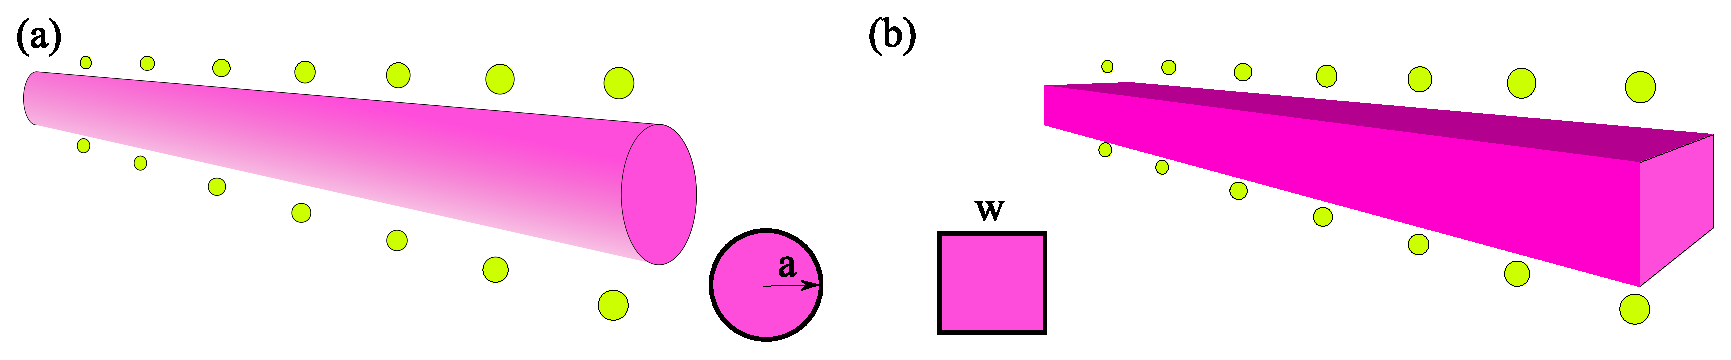
\includegraphics[width=0.89\linewidth]{../media/Figs/fiberwg_withatoms}}
\caption[Trap atoms along a nanofiber and a square waveguide.]{Diagram of Trap atoms along a nanofiber (a) and a square waveguide (b). Insets are the cross sections of the two waveguide geometries.
In this dissertation, we set the radius of the nanofiber as $ a=225 $ nm and the width of the square waveguide as $ w=300 $ nm. }\label{fig:fiberwg_withatoms}
\end{figure}

Comparing these nanophotonic configurations with a free-space atom-light quantum interface, the tight confinement of the waveguide modes provide a stronger and uniform coupling between atoms and light~\cite{Qi2016}.
%, and all atoms could be designed to sit in the same field environment, which provides a better mode matching condition. 
In fact, when the free-space trapping and probing configuration is used, one has to compromise a tradeoff in the following scenarios~\cite{Baragiola2014}.
%between enhancing the coupling to one atom while trapping less atoms or to trap more atoms yet with a weaker coupling on every atom~\cite{Baragiola2014}.
%as a quantum interface, there is a dilemma to enhance the atom-light coupling. 
If the light is designed to enhance the coupling of atoms at the waist of the laser beam, fewer atoms can be coupled to the light. 
If the light is designed to couple to as many atoms as possible, then the coupling per atom will be weak. %(or optical depth\index{optical depth} (OD) per atom)
%A tradeoff between enhancing the coupling to one atom or to all atoms has to set~\cite{Baragiola2014}.
The waveguide platforms do not have this problem, and one can multiply the coupling strength per atom for all trapped atoms. 
The coupling strength can be characterized in terms of cooperativity.

Nevertheless, the nanowaveguide platforms bring in new challenges. 
For example, due to the anisotropy of modes, the atom-light interactions become complicated. 
The alignment-dependent spontaneous emission rates of atoms have been observed in laboratories~\cite{Solano2017Alignment}. 
This new phenomenon hasn't been well considered in many of previous theoretical models in atomic optics, particularly in the context of quantum measurement and quantum control before this study.
What's worse, because of the strong field coupling, there can be strong mechanical oscillations induced by the guided probe on the trapped atoms~\cite{Wuttke2013,Solano2017Dynamics}.
These raise a new dilemma of the benefit over the damage for increasing the effective coupling between atoms and light.

We need new theories to incorporate new phenomena when using the atom-waveguide interfaces.
For quantum information applications, we also need new protocols to best use of the enhanced atom-light coupling while to avoid the disadvantages due to the enhancement itself, which limits the quality of quantum operations. 
As a concrete example, there had not been any theory quantitatively guiding faithful quantum measurements of the internal states of atoms trapped near a nanophotonic waveguides using the guided light field. 
%Without it, atom-waveguide interfaces are rather a blackbox. 
%By understanding the physics code encrypted in the nature of atom-waveguide interfaces, we could potentially gain in-depth insights towards the foundation of quantum mechanics, particularly on matter-light interactions. 
This dissertation focuses on solving these theoretical problems, with applications to quantum measurement and spin squeezing.

%\begin{figure}[ht] % This is generated by inkscape with the option ``PDF+Latex''. The PDF image is in the sub-folder ``images''. The path of the sub-folder is included by adding ``\graphicspath{{images/}}'' to zj.sty.
%   \centering
%   \def\svgwidth{0.85\textwidth} % set the image width, this is optional
%   \input{../Inputs/temperature_gradient.pdf_tex}
%   \caption[Temperature Gradient from a BEC to the Center of the Sun]{Temperature gradient from a BEC to the center of the sun.}
%   \label{fig:temperature_gradient}
%\end{figure}

\section[Quantum measurement, entanglement and spin squeezing with an atomic ensemble]{Quantum measurement, entanglement \\and spin squeezing with an atomic ensemble}
The power of quantum measurement comes from quantum entanglement between the the quantum object to be measured and the probe. 
Below, I will illustrate this statement with a simple example\footnote{Taught by Dr. Ivan Deutsch.}. Suppose a laser beam in a linearly polarized state $ \ket{\phi_L} $ is shined on an atom that is in a state of $ \ket{\phi_A} =(\ket{\uparrow}+\ket{\downarrow})/\sqrt{2} $. We want to use the laser as a probe to detect the state of the atom, where we have access to the polarization state of the light. The joint state of the atom-polarization system at the initial time $ t=0 $ can be given by
\begin{align}
\ket{\Psi(0)} &=\frac{1}{\sqrt{2}}(\ket{\uparrow}+\ket{\downarrow})\mathbin{\ket{\phi_L}}.
\end{align}
We consider an atom-light interaction defined by an evolution operator, $ \hat{U}(\tau)=e^{i\chi \hat{S}_3 \hat{J_z}\tau} $, where $ \chi $ is the coupling strength between the atom and light, $ \hat{S_3} $ is the Stokes vector operator changing the polarization state of light, and $ \hat{J}_z=\hat{\sigma}_z/2$ is the angular momentum operator for atoms. We will introduce these operators in details for sequential chapters. 
For now, we give that $ \hat{J}_z $ outputs $ +1/2 $ if the atom is in the $ \ket{\uparrow} $ state, and $ -1/2 $ if the atom is in the $ \ket{\downarrow} $ state. 
Then the joint state at time $ \tau $ becomes
\begin{align}
\ket{\Psi(\tau)}&=\frac{1}{\sqrt{2}}\left[\ket{\uparrow}e^{+i\chi \hat{S}_3\tau/2}\ket{\phi_L} 
+\ket{\downarrow}e^{-i\chi \hat{S}_3\tau/2}\ket{\phi_L} \right]\\
&=\frac{1}{\sqrt{2}}\left[\ket{\uparrow}\ket{\phi^1_L} 
+\ket{\downarrow}\ket{\phi^2_L} \right]
\end{align}
where $ \ket{\phi_L^1}=e^{+i\chi \hat{S}_3\tau/2}\ket{\phi_L} $ and $ \ket{\phi_L^2}=e^{-i\chi \hat{S}_3\tau/2}\ket{\phi_L} $ are two polarization states with the polarization axis of the light rotated by $ \pm \chi \tau/2 $, respectively. 
Therefore, the output state of the system is an entangled state. It predicts that, if the polarization state of the light is measured to be rotated by $ +\chi\tau/2 $ from the original state, then the atom is in the $ \ket{\uparrow} $ state. Otherwise, if the light is rotated by $ -\chi\tau/2 $, the atom is in the $ \ket{\downarrow} $ state. 
Therefore, the probe works as a meter for us to access to the state of the atom through the mutual entanglement. 
The sensitivity of the measurement is determined by the rotation angle of the polarization state of the light. 
In other words, to make the measurement outputs more distinguishable, we need to enhance the coupling strength of the bipartite system. 
%\qxd{Put my picture of the meter and measurement here.}

%A quantum state is so fragile that, if you measure it, you also destroy it. We can only gain partial information from one shot of measurement based on the uncertainty principle. 
%If we know the recipe to prepare the quantum state, there are two naive ways to reconstructing the quantum state: to prepare multiple copies of the quantum object and measure them sequentially in different bases; or, to measure the object multiple times by repeating the preparation processes. 
%After the seminar work by Holevo~\cite{Holevo2011Probabilistic}, we now know that the optimal quantum measurement strategy to gain more information with less destructive measurement trials is to prepare multiple copies of the object and measure all of them collectively. Various protocols have been implemented on different quantum systems~\cite{Massar2005Optimal,Derka1998Universal,Jones1994Fundamental}. Particularly, the quantum non-demolition (QND) measurement technique has been implemented on atomic systems~\cite{Smith2003a,Smith2004Continuous}.
%The continuous measurements allowed by QND measurement techniques have paved a solid foundation to recent hot fields including quantum state tomography~\cite{Smith2013,SosaMartinez2016Quantum}, quantum process tomography~\cite{Baldwin2014Quantum}, quantum compressed sensing~\cite{Smith2013} and so on. 

%Moreover, as a result of continuous measurement on a collective state, a squeezed state can be generated. 
Assume we have $ N_A $ atoms initially all prepared in the superposition state as above, $ \ket{\phi_A} = \left[(\ket{\uparrow}+\ket{\downarrow})/\sqrt{2} \right]^{\otimes N_A}$, which is called a spin coherent state\index{state!spin coherent state}.
%Based on the uncertainty principle, the spin coherent state has a possibility distribution for all eigenstate of the ensemble. 
With all atoms coupled with a probe and letting the joint system evolve in time $ \tau $ under the evolution operator introduced above, we replace the single Pauli operator with the collective spin operator $\hat{J}_z=\sum_i^{N_A}\hat{\sigma}_z^{(i)}/2  $. Upon measuring the probe, the uncertainty of the measurement result can be reduced compared to the initial state.
We call this process as spin squeezing. The state generated is called a spin squeezed state\index{state!spin squeezed state}.
The mechanism of measurement-induced squeezing is usually called measurement backaction\index{measurement backaction}.

\begin{figure}[!tpb] % Poincare sphere.
   \centering\makebox[\textwidth]{
   %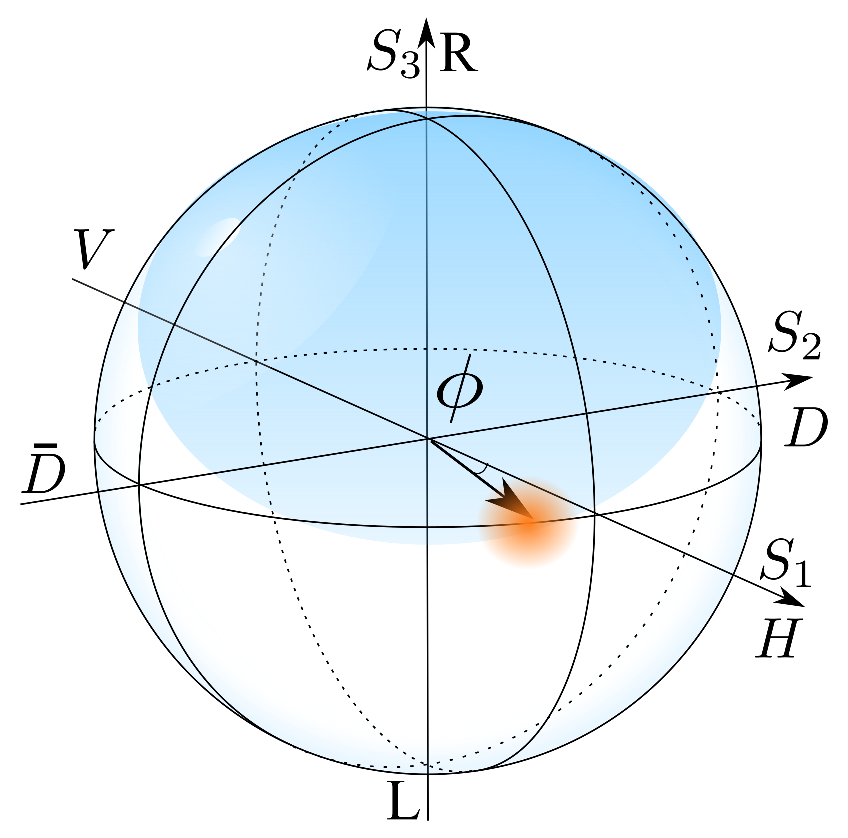
\includegraphics[width=0.55\textwidth]{../media/Figs/poincaresphere_initialS1_Faradayrot_crystal}}
   \begin{minipage}[h]{\linewidth}
    %\begin{tabular}{*{2}{b{0.2\textwidth-2\tabcolsep}}}
     \subfloat[h][]{
       %% This file was created by matlab2tikz.
%
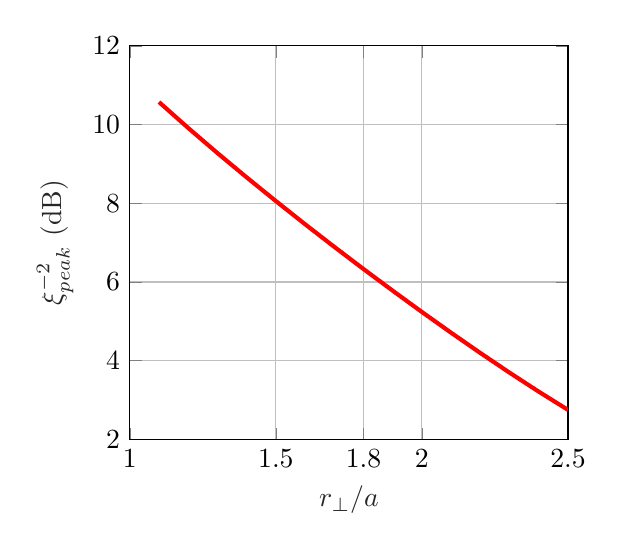
\begin{tikzpicture}

\begin{axis}[%
width=5.565cm,
height=5cm,
at={(0cm,0cm)},
scale only axis,
xmin=1.0000,
xmax=2.5000,
xtick={1.0000,1.5000,1.8000,2.0000,2.5000},
xlabel style={font=\color{white!15!black}},
xlabel={$r_\perp/a$},
ymin=2.0000,
ymax=12.0000,
ylabel style={font=\color{white!15!black}},
ylabel={$\xi^{-2}_{peak}$ (dB)},
axis background/.style={fill=white},
xmajorgrids,
ymajorgrids
]
\addplot [color=red, line width=1.5pt, forget plot]
  table[row sep=crcr]{%
1.1000	10.5712\\
1.2000	9.9128\\
1.3000	9.2762\\
1.4000	8.6588\\
1.5000	8.0571\\
1.6000	7.4685\\
1.7000	6.8935\\
1.8000	6.3307\\
1.9000	5.7799\\
2.0000	5.2394\\
2.1000	4.7118\\
2.2000	4.1974\\
2.3000	3.6980\\
2.4000	3.2157\\
2.5000	2.7531\\
};
\end{axis}
\end{tikzpicture}%
       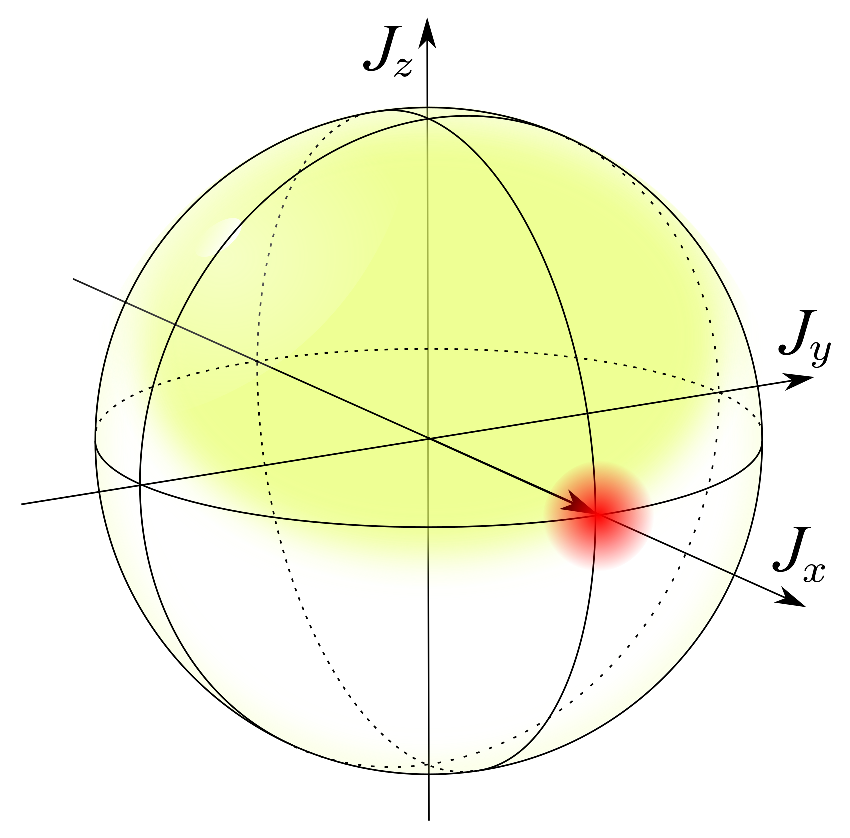
\includegraphics[width=0.3\linewidth]{../media/Figs/blochsphere_initialxJxyz_coherent}
       \label{fig:blochsphere_initialxJxyz_coherent}
       }
       \hfill
     \subfloat[h][]{
         \label{fig:blochsphere_initialxJxyz_squeezed}
         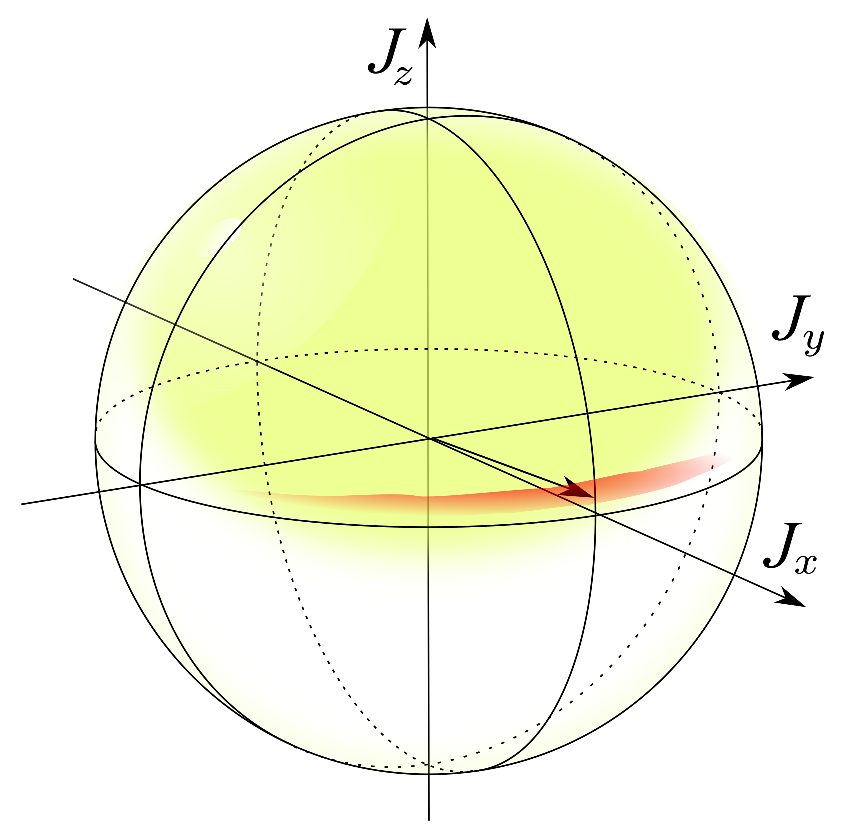
\includegraphics[width=0.3\linewidth]{../media/Figs/blochsphere_initialxJxyz_squeezed}
         %% This file was created by matlab2tikz.
%
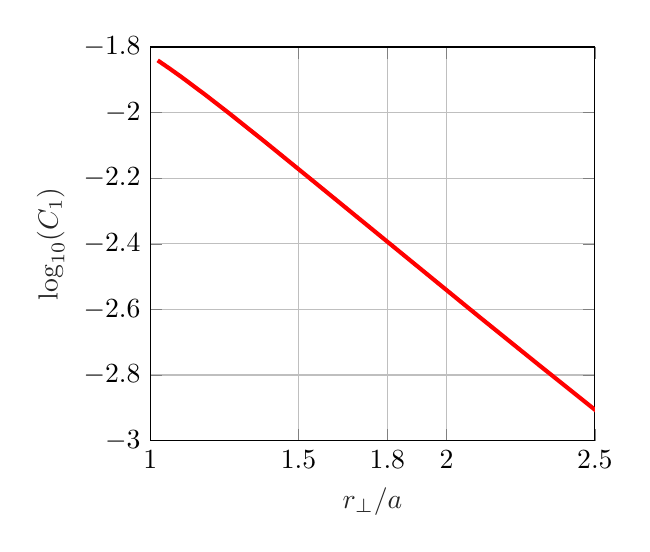
\begin{tikzpicture}

\begin{axis}[%
width=5.647cm,
height=5cm,
at={(0cm,0cm)},
scale only axis,
xmin=1.0000,
xmax=2.5000,
xtick={1.0000,1.5000,1.8000,2.0000,2.5000},
xlabel style={font=\color{white!15!black}},
xlabel={$r_\perp/a$},
ymin=-3.0000,
ymax=-1.8000,
ylabel style={font=\color{white!15!black}},
ylabel={$\log_{10}(C_1)$},
axis background/.style={fill=white},
xmajorgrids,
ymajorgrids
]
\addplot [color=red, line width=1.5pt, forget plot]
  table[row sep=crcr]{%
1.0251	-1.8409\\
1.0653	-1.8658\\
1.1055	-1.8917\\
1.1859	-1.9459\\
1.2663	-2.0022\\
1.3869	-2.0891\\
1.5477	-2.2073\\
2.1106	-2.6230\\
2.3116	-2.7696\\
2.5126	-2.9148\\
};
\end{axis}
\end{tikzpicture}%
         }\hfill
     \subfloat[h][]{
            %% This file was created by matlab2tikz.
%
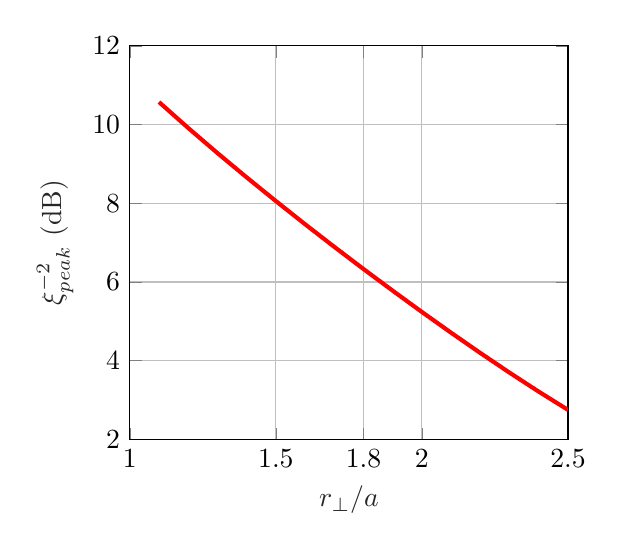
\begin{tikzpicture}

\begin{axis}[%
width=5.565cm,
height=5cm,
at={(0cm,0cm)},
scale only axis,
xmin=1.0000,
xmax=2.5000,
xtick={1.0000,1.5000,1.8000,2.0000,2.5000},
xlabel style={font=\color{white!15!black}},
xlabel={$r_\perp/a$},
ymin=2.0000,
ymax=12.0000,
ylabel style={font=\color{white!15!black}},
ylabel={$\xi^{-2}_{peak}$ (dB)},
axis background/.style={fill=white},
xmajorgrids,
ymajorgrids
]
\addplot [color=red, line width=1.5pt, forget plot]
  table[row sep=crcr]{%
1.1000	10.5712\\
1.2000	9.9128\\
1.3000	9.2762\\
1.4000	8.6588\\
1.5000	8.0571\\
1.6000	7.4685\\
1.7000	6.8935\\
1.8000	6.3307\\
1.9000	5.7799\\
2.0000	5.2394\\
2.1000	4.7118\\
2.2000	4.1974\\
2.3000	3.6980\\
2.4000	3.2157\\
2.5000	2.7531\\
};
\end{axis}
\end{tikzpicture}%
            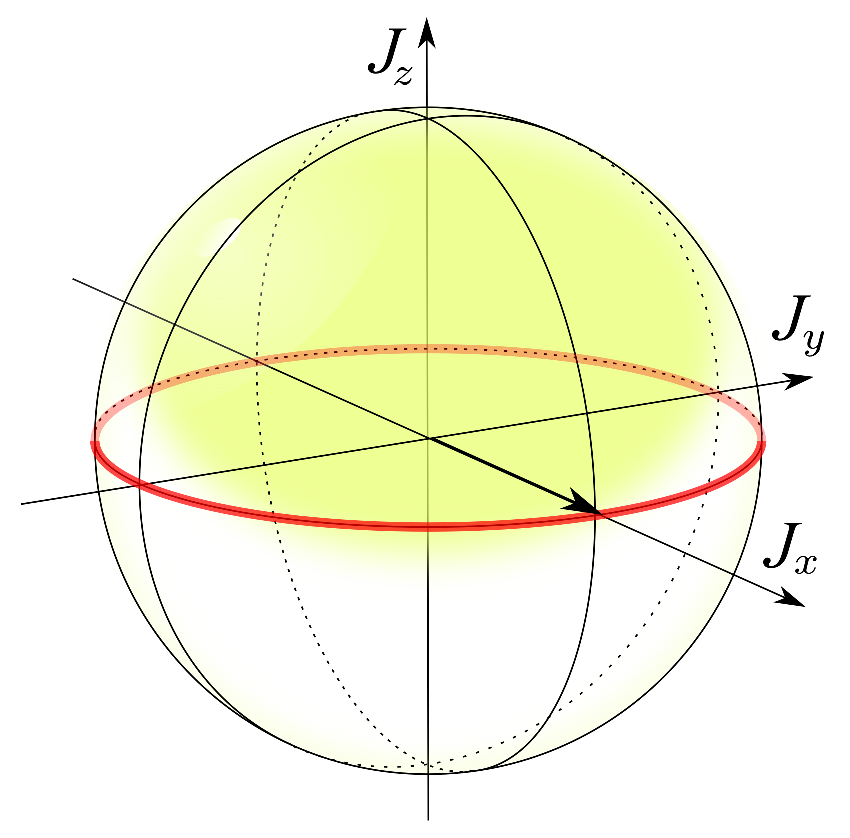
\includegraphics[width=0.3\linewidth]{../media/Figs/blochsphere_initialxJxyz_Dicke}
            \label{fig:blochsphere_initialxJxyz_Dicke}
            }
   \end{minipage}}
   \caption[Coherent state, spin squeezed state and Dicke state on the Bloch sphere.]{Coherent state (a), spin squeezed state (b) and Dicke state (c) on the Bloch sphere. 
   The red shadows indicate the probability distributions and uncertainties on the Bloch sphere defined by the collective spin $ \hat{\mathbf{J}} $ vector operator.
   }
   \label{fig:collectivestatesonblochsphere}
\end{figure}


It has been proven by Caves that a squeezed state is crucially useful quantum resource for precise measurements using light~\cite{Caves1981Quantum,Caves1982Quantum}. 
Thus was generalized by Wineland and coworker to employ spin squeezing for Ramsey spectroscopy for use in atomic precision measurement.  
In some sense, how much a state is squeezed determines how precise a quantum measurement can be. 
When we plot a squeezed collective state on a Bloch sphere that represents the probability distribution of the state, the uncertainty region is squeezed from the initial spin coherent state (see Fig.~\ref{fig:collectivestatesonblochsphere}).  
When the squeezing is weak, the squeezed state can be regarded as a Gaussian state, which is dominated by pairwise quantum correlations of atoms in the ensemble. 
If the squeezing is on the order of the radius of the Bloch sphere, the collective state become non-Gaussian, which is usually dominated by many-body correlations~\cite{Strobel2014,Dubost2012Efficient}. 
To the extreme, if the state wrap around the Bloch sphere as a line of circle, it is called a Dicke state~\cite{Dicke1954}. 
Using a non-Gaussian state for quantum metrology, quantum communications, and in general, for quantum information processing, can offer a better performance than using a Gaussian state~\cite{Strobel2014,Ji2016Quantum,Ghose2007Non,Borelli2016Quantum}.
However, a highly non-Gaussian state of an atomic ensemble is still difficult to produce. 

One of the goals of spin squeezing is to generate a non-Gaussian state, to make a quantum-measurement--induced squeezed state more useful~\cite{Buono2013Quantumness}. 
For an ensemble of atoms, the radius of the Bloch sphere is defined by the total number of atoms and the dimension of the internal states of an atom. 
In addition, the measurement backaction that generates squeezing is proportional to the coupling strength between atoms and probe.
Therefore, the key to generate a highly squeezed state is to enhance the coupling strength between atoms and light with a given number of atoms. 
We consider the interface of nanophotonic waveguide-trapped atoms towards this goal.




%\section{The philosophy of cooperativity}
%
%For single atom and many.
%
%In general, the evolution of the polarization state of the light in the context of atom-light interaction, characterized by the Stokes vector $\mathbf{S} $ on the \Poincare sphere, may be governed by the following equation~\cite{Deutsch2010a}:
%\begin{align}
%\dt{\mathbf{S}} &= \mathbf{\Theta}\times\mathbf{S}_{in}
%\end{align}
%where the rotating angle vector around $ S_i $ axis can be given by
%\begin{align}
%\Theta_i &\propto \mathrm{OD}\frac{\Gamma}{2\Delta} =N_A\left( \frac{\sigma_0}{A}\right) 
%\left(\frac{\Gamma}{2\Delta}\right),
%\end{align}
%where OD is the total optical depth of the atoms\index{optical depth}, $ N_A $ is the number of atoms, $ \Gamma $ is the spontaneous decay rate of an atom, and $ \Delta $ is the detuning relative to the atomic resonance. 
%We have also defined the OD per atom in terms of the on-resonant cross section of the atom $ \sigma_0 $ and the effective mode area of the optical field at the atom position $ A $ by
%\begin{align}
%\frac{\mathrm{OD}}{N_A} &= \frac{\sigma_0}{A}.
%\end{align}
%Note that, in the free-space trapping case, an effective number of atoms is used to replace $ N_A $, since atoms are not equally coupled to the light.
%In the waveguide case, the formula of OD per atom above applies perfectly. However, there is a hidden secret. 
%
%We realize that the effective mode area can simply written as
%\begin{align}
%A= \frac{A_{\rm interaction}^2}{A_{\rm in}},
%\end{align}
%where $ A_{\rm interaction} $ is the effective area for the interaction depending on the polarization of the light and the internal structure of the atoms, and $ A_{\rm in} $ is the effective mode area of the total local field at the atom positions. 
%In addition, for QND measurements, we will show that the concept of cooperativity per atom, $ C_1 $, is essentially the OD per atom, and we have the following relations 
%\begin{align}
%C_1 =\frac{\kappa}{\gamma_s} \propto \frac{\sigma_0 A_{\rm in}}{A_{\rm interaction}^2},
%\end{align}
%where $ \kappa $ is the measurement strength--indicating the good effect we want, and $ \gamma_s $ is the characteristic photon scattering rate--indicating the damaging effect in the quantum measurement process. 
%Given that $ A_{\rm in} $ is associated with decoherence and such with $\gamma_s  $, we conclude that $ A_{\rm interaction} $ fully defines the useful interaction effects we target for. 
%Both $ A_{\rm in} $ and $ A_{\rm interaction} $ are geometry-dependent, while $ A_{\rm interaction} $ also depends on the internal state of the atoms. 
%Therefore, using nanophotonic waveguides with a given atomic state, one can enhance the atom-light coupling by optimizing the geometry defined by the boundary shape of the waveguide, the atoms' transverse location, the choice of quantization axis, and the polarization direction of the light. 
%In fact, we show protocols that enhance the atom-light coupling by placing the atoms at the azimuthal angle position that has the weakest field to the atom, which is counter-intuitive in the traditional way to think about atom-light coupling. But it is optimal--in the sense that it maximizes the good effect while minimizes the bad effect--and feasible to implement using the nanophotonic waveguides.
%This type of design could potentially solve the dilemma that the mechanical oscillations and other bad effects hindering manipulating atoms grow with the increase of atom-light coupling as people have thought. 
%All of these degrees of freedom of optimization are degenerate in free-space atom-light interfaces and are locked into the geometry-independent effective mode area $ A $--this is one of the main messages we have learned in studying this subject.  
%
%
%Techniques will advance and our knowledge will gain when contradictories are solved.
%We will elucidate these ideas to solve the traditional contradictories with the atom-waveguide interfaces and provide some concrete quantum information protocols in the following chapters. 

%\begin{figure}[ht] %This figure is drew by Inkscape using the very handy tool 'parametric curves'. The fringe is the hard part, and I don't know how to do it elegantly (I just use a combination of 'cheating' methods to generate it). However, there is one command called '\pgfdeclarefunctionalshading' in the tikZ package which could be helpful. But, unfortunately, it requires knowing how to write PostScript codes.
%   \centering
%   \def\svgwidth{0.85\textwidth}
%   \input{../Inputs/double_well_interfer.pdf_tex}
%   \caption[A Double-Well Atom Interferometer]{A double-well atom interferometer~\cite{shin_atom_2004}: (i)~cool the atoms trapped in a single-well potential to form a BEC; (ii)~split the condensate by slowly deforming the single-well potential to a double-well potential; (iii)~apply ac Stark shift potentials to either of the two separated condensates; (iv)~turn off the double-well trapping potential, and let the condensates ballistically expand, overlap, and interfere; and (v)~take an absorption image.}
%   \label{fig:double_well_interfer}
%\end{figure}


\section{Outline of This Dissertation}
In Chapter 2, we introduce the basic properties of the waveguides to be used in modeling polarization spectroscopy measurements. 
These includes the description of polarizations using the Stokes vectors, the properties of the eigenmodes of the waveguides, the dyadic Green's function due to the radiation from atoms near a waveguide and the evolution of the guided modes of waveguides. 
We relate the phase shift of one guided mode of the waveguide with the spontaneous emission rate of the atoms. 
With the changes of the relative phase and amplitudes of two orthogonal guided modes, we can fully describe the polarization transformation of the guided light.
Everything in this chapter is modeled in the classical picture. 
That is, we treat the electromagnetic wave as a classical field and treat atoms as dipoles.

In Chapter 3, we discuss the modification of the spontaneous emission rate (or decay rate) of atoms by generalizing some of the classical results introduced in Chapter 2 to the quantum regime. 
We introduce the polarizability tensor operators of atoms to describe the hyperfine state of atoms. 
We model the spontaneous emission rates of atoms in the presence of a dielectric waveguide using the Green's function language. 
Using a modal decomposition, we separate the decay rates into the guided and unguided mode components, which are responsible to the polarization transformation of the light and the modification of atomic properties due to the waveguide. 
We use the example of the decay rate calculation for a free dipole in vacuum to introduce the equivalent dipole method for studying the Purcell effect.
With this method, we first develop the theory for calculating the modified spontaneous decay rate of classical dipoles due to waveguides without considering the internal structure of atoms. 
Then we generalize this theory to include the internal structure of atoms to calculate the modified decay rates of alkali atoms. 
In the dispersive regime, we find the cases where we can ignore the modification of the decay rates of atoms due to the waveguide.
A geometric explanation of the unique features of waveguide interfaces compared to optical fields in vacuum is given at the end of the chapter to cast some insights on designing a good waveguide geometry for enhancing atom-light coupling. 

Chapter 4 introduces the Hamiltonian and characteristics of QND measurement and the measurement-induced spin squeezing effect. We define the clock states and the stretched states of individual alkali atoms and some collective states of an atomic ensemble, which will be used for designing our QND measurement and spin squeezing protocols that follow. 

Chapter 5 is based on our publication, Ref.~\cite{Qi2016}, which establishes a general theory to describe atom-light interactions on a nanophotonic waveguide platform (mainly taking the nanofiber dispersive interface as an example) with applications to QND measurement and spin squeezing based on the birefringence interactions. 
We develop an input-output formalism using the Green's function language and solve the light response problem due to atoms near a nanofiber in the Heisenberg-Langevin picture. 
Then we apply our theory to design protocols for atom number counting, QND measurement and spin squeezing by optimizing the choice of quantization axis and finding a magic frequency to cancel noise terms in the interaction Hamiltonian.
We show that $ \sim 4.7 $ dB of squeezing are attainable with $ 2500 $ atoms trapped near a realistic nanofiber, which is a great improvement for small numbers of atoms, and could lead to generation of non-Gaussian states with applications to precise atomic clocks.

Chapter 6 is based on our publication, Ref.~\cite{Qi2017Enhanced}, which is about further enhancement of the cooperativity per atom in the context of Faraday-effect--based QND measurement and spin squeezing with waveguides. 
Such a geometry is useful in the context of creating spin squeezed states for magnetometry.
We consider both a nanofiber and a square waveguide as examples for designing the protocol. 
We define the cooperativity formula for the QND measurement, which enables us to find the optical geometry to maximize the squeezing effect. 
In order to calculate the spin squeezing parameter, we develop a set of stochastic master equations using microscopic operators and find the relations between our microscopic operators and the collective operators that define the squeezing parameter. We compare the squeezing using the Faraday effect against the birefringence effect, and using nanofibers verse square waveguides. We show the cooperativity we define is the key parameter to guide the design of waveguides and the measurement geometry. We also find the counter-intuitive result that the optimal azimuthal positions of atoms to enhance the squeezing effect is where the local field is the weakest.

We conclude and provide some suggestions for future works in Chapter 7.

\section{Other Works}
In addition to the works presented in this dissertation, I have been also working on the following topics during my PhD study at UNM.

1. Studies on the collective radiation effect of atoms near a nanophotonic waveguide. 
A summer project has been done and is still on-going in collaboration with Prof. Perry Rice from the Miami University at Ohio. 
One problem we were worried about for my dissertation study is that the collective photon emission of atoms may be enhanced in presence of a waveguide which may make our problem more complicated~\cite{Asenjo-Garcia2017Atom,Asenjo-Garcia2017Exponential}.
Through our summer project study, we conclude that, in the dispersive regime, the collective effect can be safely ignored as we wish, and the assumption of pairwise symmetry of atoms can be applied to the calculation of collective spin dynamics. 
We also worked on some ideas proposed by Prof. Rice to explain collective emission rates of atoms in presence of a nanofiber, which were observed at the laboratories of Prof. Luis Orozco and Prof. Steve Rolston at the University of Maryland. 

2. To design a probe scheme so that the tensor light shifts are canceled completely for the QND measurement and spin squeezing protocol. 
In our paper, Ref.~\cite{Qi2017Enhanced}, we assume the tensor light shift of atoms is negligible or has been canceled using experimental techniques developed for the free-space atom-light interfaces~\cite{Montano2015Quantum}. 
However, no one has done the modeling and simulations for the nanophotonic waveguide cases to-date, in which the decay rates of atoms are state-dependent and are no longer degenerate for different quantum transitions.
Using the result of Chapter 3, I have developed a draft model for finding a magic frequency to cancel the tensor light shift with two-color probes and for calculating the spin squeezing dynamics including the modification of decay rates. 
%But the math is messy, and no concrete result obtained yet. I plan to finish this project and incorporate my formalism with our colleagues at CQuIC and outside for a general theory of continuous measurement and control using the atom-waveguide interfaces introduced in this dissertation. 


%</tag>
%###################################################################################
\bibliographystyle{../styles/abbrv-alpha-letters-links}
\bibliography{../refs/Archive,../chap5/Nanofiber}
%%%%%%%%%%%%%%%%%%%%%%%%%%%%%%%%%%%%%%%%%%%%%%%%%%%%%%%%%%%%%%%%%%%%%%%%%%%%%%%%%%%%%

\printindex
%\cleardoublepage
%\thispagestyle{plain}
%\phantomsection
%\printindex{ai}{Author Index}
%\chaptermark{Author Index}
%\thispagestyle{plain}
%\printindex{si}{Subject Index}
%\chaptermark{Subject Index}
\end{document}

%\meaning\tmp
\ExecuteMetaData[../chap2/WaveguideInterface.tex]{waveguideinterface}
%\CatchFileBetweenTags\temptoken{../chap2/WaveguideInterface.tex}{waveguideinterface}\the\temptoken
%\documentclass[fleqn, final]{../styles/unmphythesis}
\usepackage{../styles/qxd}
\renewcommand{\thechapter}{2}
%\newcommand{\thechapter}{1}

\makeindex
\begin{document}

%<*waveguideinterface>

\chapter{Atom-waveguide interfaces}
\section{Introduction}
In this chapter, we look at the case that only one atom is trapped nearby a waveguide. As will be discussed later, in the dispersive regime, the interaction from many atoms can be treated as a sum of the interactions from all individual atoms. To be specific, for this chapter, we consider the following scenario: a laser beam propagates through a waveguide along $ z $ direction; an alkali atom (cesium, for example) is trapped at $ \mathbf{r}_{\rm atom} =\mathbf{r}'$ in the evanescent field of the waveguide~\footnote{We will use the prime ($ ' $) notation to indicate the position of a photon emitter.} and responds to the guided optical field dispersively. In the dynamics, the atom can be treated as an optical dipole that adiabatically eliminates from an excited state to the ground state as an effective two-level system. The light, on the other hand, experiences dispersive phase shift and usually negligible intensity attenuation afterwards. Effectively, the presence of the atom outside of the waveguide changes the index of refraction\index{index of refraction} of the waveguide. 
The dispersive light shift applies when the saturation parameter is small,
\begin{align}
s=\frac{\Omega^2/4}{\Delta^2+\Gamma^2/4}\ll 1,
\end{align}
where $ \Omega $ is the Rabi frequency, $ \Gamma $ is the spontaneous emission rate of the atom, and $ \Delta=\omega-\omega_{eg} $ is the probe detuning from the atomic resonance frequency $ \omega_{eg} $ as a two-level system with the probe's frequency set to be $ \omega $. 

We will first introduce the experimental setup in characterizing the dispersive light shift interaction, which is called polarization spectroscopy; then we will develop a general theory in the language of Green's function to formulate the atom-light interaction mainly from the semi-classical perspective where the light is treated as a continuous wave while the atom has discrete level structures. 
At the end of this chapter, we will conclude with geometric explanations on the unique features and advantages of using a nanophotonic waveguide interface to implement atom-light coupling over the free-space interface commonly employed in previous experiments.

\section{Polarization spectroscopy and dispersive light shift measures}

As a result of the atom-light interaction, the polarization of the light will experience one of the two optical effects, the birefringence effect and the Faraday effect~\cite{Jackson1975}, or a mixture of the two effects. 

In free space, light becomes transverse. The polarization state of light can be fully described by the amplitudes and relative phase of two orthogonal electric field components, $ \mathbf{E}_x $ and $ \mathbf{E}_y $. That is we write the electric field of the light to be $ \mathbf{E}=\mathbf{E}_x+\mathbf{E}_y$ and the two orthogonal components
\begin{align}
\mathbf{E}_x &= E_{0x} e^{i(kz-\omega t)+i\phi_x}\\
\mathbf{E}_x &= E_{0y} e^{i(kz-\omega t)+i\phi_y},
\end{align}
where $ E_{0x} $ and $ E_{0y} $ are the amplitudes, and $ \phi_x $ and $ \phi_y $ are the phases of the $ x $- and $ y $-components of the wave, respectively, while $ \mathbf{e}_x $ and $ \mathbf{e}_y $ are the respective unit vectors along the positive $ x $- and $ y $-axes. 


To describe the polarization state of the light, there are many equivalent formalisms, including ~\cite{Mecozzi2011Unified}

The change of polarization of the light can be measured using the polarization spectroscopy technique~\cite{Deutsch2010a,Salvail2013}.

\section{Photon emission in the perspective of Green's function method}

We assume that the waveguide is a infinite long cylinder with a radium of $ a $ (in our cases, $ a<\lambda $, where $ \lambda $ is the wavelength of the laser beam). The laser beam propagating in the waveguide generates an electrical field given by
\begin{equation}
\mathbf{E}_0(\br,t)=\boldsymbol{\mathcal{E}}_0(\br)e^{-i\omega t} %+\frac{1}{2}\mathrm{c.c.}
=\mathcal{E}_0(\br)\mathbf{u}_0(\br)e^{-i\omega t}, %+\frac{1}{2}\mathrm{c.c.},
\label{Ert0}
\end{equation}
where $\omega$ is the angular frequency and $\boldsymbol{\mathcal{E}}_0(\br)=\mathcal{E}_0\mathbf{u}_0$ is the positive-frequency electric field envelope,
with $\mathcal{E}_0(\br)$ and $\mathbf{u}_0(\br)$ being the field amplitude and the polarization vector at $ \br $, respectively.
In general, $\mathcal{E}(\br)$ is a complex scalar and $\mathbf{u}(\br)$ is a complex unit vector. 

We assume the waveguide is a linear medium with no absorption to the traveling wave. The refractive intrinsic index\index{refractive index} of the waveguide can be given by
\begin{align}
n_0(\br) = \begin{cases} 
n_1=1.45, &\quad r_\perp \leq a,\\
n_2=1, &\quad r_\perp >a,
\end{cases} 
\end{align}
where we have set the $ z $-axis to be the symmetric center of the waveguide and $ r_\perp =\sqrt{x^2+y^2} $. We would like to determine the form of the scattered field $ \boldsymbol{\mathcal{E}}_s(\br) $, and the total field $ \boldsymbol{\mathcal{E}}(\br)=\boldsymbol{\mathcal{E}}_0(\br)+\boldsymbol{\mathcal{E}}_s(\br) $. Formally, the total time-dependent electrical field can be rewritten as 
\begin{equation}
\mathbf{E}(\br,t)=\boldsymbol{\mathcal{E}}(\br)e^{-i\omega t} %+\frac{1}{2} \mathrm{c.c.}
=\mathcal{E}(\br)\mathbf{u}(\br)e^{-i\omega t}, %+\frac{1}{2}\mathrm{c.c.},
\label{Ert}
\end{equation}

The total field will satisfy the \textit{Maxwell-Helmholtz equation}\index{Maxwell-Helmholtz equation} that
\begin{align}
\left[ -\nabla\times\nabla\times+\frac{\omega^2}{c^2}n^2(\br) \right] \boldsymbol{\mathcal{E}}(\br) &=0. \label{MaxwellHelmholtz0}
\end{align}
Notice that the total index of refraction $ n(\br) $ we used above has already included the scattering effect caused by the atom on the waveguide, which usually has a complicated form. It is not in general possible to solve the differential equation as given above. The solution to the Maxwell-Helmholtz equation\index{Maxwell-Helmholtz equation} with $ n(\br)=1 $, however, are much more tractable, so we subtract $ \frac{\omega^2}{c^2} \boldsymbol{\mathcal{E}}(\br)$ to each side of Equ.~\ref{MaxwellHelmholtz0} and add $ \frac{\omega^2}{c^2}n(\br) \boldsymbol{\mathcal{E}}(\br) $ to give (in Gauss unit)
\begin{align}\label{eq:Maxwellwithsource}
\left[\! -\! \nabla\!\times\!\nabla\!\times + \frac{\omega^2}{c^2} \right]\! \boldsymbol{\mathcal{E}}(\br) &=\! -i4\pi\frac{\omega}{c^2} \mathbf{J}(\br) =\! -4\pi\frac{\omega^2}{c^2} \mathbf{P}(\br)=\! -4\pi \frac{\omega^2}{c^2} \tensor{\chi}(\br)\! \cdot\! \boldsymbol{\mathcal{E}}(\br),
\end{align}
where we have defined the current $ \mathbf{J}(\br)=\pp{\mathbf{P}}{t}=-i\omega\mathbf{P}(\br)=-i\omega \tensor{\chi}(\br)\cdot \boldsymbol{\mathcal{E}}(\br) $ with electric susceptibility\index{electric susceptibility} $ \tensor{\chi}(\br)=[\tensor{\varepsilon}_r(\br)-\mathbbm{1}]/4\pi = \sum_{\br'}\delta(\br-\mathbf{r}')\tensor{\alpha} \, (\br')$ \footnote{We have used Gauss units here. In SI units, the corresponding relationship is $ \tensor{\chi}(\br)=\tensor{\varepsilon}(\br)/\varepsilon_0-\mathbbm{1} = \sum_{\br'}\delta(\br-\mathbf{r}')\tensor{\alpha} \, (\br')$ and $\tensor{\chi}^{SI}=4\pi\tensor{\chi}^{G}  $. The factor of $ 4\pi $ defines the transformation between the SI and Gauss units. } where $\tensor{ \varepsilon}_r(\br) $ is the relative permittivity\index{permittivity!relative permittivity} or dielectric constant\index{dielectric constant} at $ \br $ and $ \tensor{\alpha} $ is the polarizability\index{polarizability} of the atoms at $ \br' $. Specifically, using dipole approximation, the polarizability $ \mathbf{P}(\br)=\sum_{\br'}\delta(\br-\br')\mathbf{d}(\br')=\sum_{\br'}\delta(\br-\br')\tensor{\alpha} \, (\br')\cdot \boldsymbol{\mathcal{E}}(\br) $ where $ \mathbf{d}(\br') $ is the induced dipole moment at $ \br' $.
%~\footnote{\textcolor{red}{This electric susceptibility needs to be fixed.} Aside on multiple atoms case: if there are many atoms distributed along the waveguide, we can in general use 
%$\boldsymbol{\chi}(\br)=\sum_i \delta(\br-\br_{i})\boldsymbol{\alpha}^i$,
%where $ i $ counts over all atoms.}. 

Noting that the terms on all the right-hand sides of Equ.~\eqref{eq:Maxwellwithsource} are the generator or source for the electromagnetic field. In absence of the generators, the field will propagate in the background medium (free-space) as described by the left-hand side of the equation. In other word, the generators in terms of $ \mathbf{J}(\br) $, $ \mathbf{P}(\br) $ or $ \boldsymbol{\chi}(\br) $ describes the property of the fiber as a medium other than the vacuum. In contrast, if we consider the fiber as the background medium and the atoms outside the fiber as sources of electromagnetic field emitters, we can formally rewrite the chromatic wave equation as 
\begin{align}\label{eq:Maxwellwithsource2}
\left[\! -\! \nabla\!\!\times\!\nabla\!\!\times + n^2\!(\br)\frac{\omega^2}{c^2} \right]\!\! \boldsymbol{\mathcal{E}}(\br) &\!=\! -i4\pi\! \frac{\omega}{c^2}\! \mathbf{J}(\br) \!=\! -4\pi\! \frac{\omega^2}{c^2}\! \mathbf{P}(\br)\!=\! -4\pi\! \frac{\omega^2}{c^2}\! \tensor{\chi}(\br)\! \cdot\! \boldsymbol{\mathcal{E}}(\br),
\end{align}
where the only difference from Equ.~\eqref{eq:Maxwellwithsource} is that we bring in the $ n(\br) $ as the index of refraction of the background medium instead of using $ n(\br)=1 $ for the homogeneous vacuum as the background medium. This has also been derived in the appendix (see Equ.~\eqref{eq:waveeqGaussU}) from the Maxwell equation for general cases. We will use Equ.~\eqref{eq:Maxwellwithsource2} to study the optical properties of the waveguide in presence of atoms outside. 

The Equ.~\eqref{eq:Maxwellwithsource2} above has a source term 
\begin{align}
\tensor{S}(\br)=\tensor{\chi}(\br),% \boldsymbol{\mathcal{E}}(\br),
\end{align}
and can be solved by solving the corresponding dyadic Green functions\index{Green function!dyadic Green function} in the frequency domain\footnote{If we define the Green's function by $\left[ -\nabla\times\nabla\times + n^2\frac{\omega^2}{c^2} \right] \GFT(\br,\br') = \delta^{(3)}(\br-\br')\unittensor$, then the source term of the corresponding field will be $\tensor{\bf S}(\br)=-4\pi \frac{\omega^2}{c^2} \tensor{\boldsymbol{\chi}}(\br)$, which has a $4\pi\omega^2/c^2$ factor compared to our definition in the text. Similarly, the $4\pi\omega^2/c^2$ factor will be carried over to other quantities as well. }
\begin{align}
\left[ -\nabla\times\nabla\times + n^2\frac{\omega^2}{c^2} \right] \GFT(\br,\br') &= -4\pi \frac{\omega^2}{c^2}\delta^{(3)}(\br-\br')\unittensor. \label{eq:dyadicGF}
\end{align}

Without loosing generality, we consider a simple free-space case that there is no net charge and current in a vacuum medium. The wave equation can be given in Equ.~\eqref{eq:freespacewaveeq} with $ n=1 $, where we have replaced $ -\nabla\times\nabla\times $ with $ \nabla^2 $ from Equ.~\eqref{eq:Maxwellwithsource2}. As a result, all vector components of the field vectors are independent to each other. The corresponding Green function equation for this problem becomes a scalar equation,
\begin{align}
(\spp{}{x_i} + k^2) G_i(\br,\br')=-4\pi \frac{\omega^2}{c^2}\delta(\br-\br'), 
\end{align}
where $ x_i $ are the coordinate components and $ G_i(\br,\br') $ is the scalar Green function responding to a unit source with only $ x_i $ field component. 
The only physical solution for the scalar Green function\index{Green function} in free space is 
\begin{align}
G_0(\br,\br') =k^2\frac{e^{\pm i\mathbf{k}\cdot (\mathbf{r}-\br')}}{|\br-\br'|},
\end{align}
where we only look at the \textit{positive} signed solution for our example. 

Assuming the boundary contributions vanish, we may have
\begin{align}
\boldsymbol{\mathcal{E}}(\br) &= \boldsymbol{\mathcal{E}}_0 (\br) + \int_V \tensor{S}(\br') \! \cdot\! \boldsymbol{\mathcal{E}}(\br') \frac{e^{i\mathbf{k}\cdot \mathbf{R}}}{R} \mathrm{d}^3 r', \label{Etotal0}
\end{align}
where $ \boldsymbol{\mathcal{E}}_0 (\br) $ is the homogeneous Maxwell-Helmholtz equation\index{Maxwell-Helmholtz equation!homogeneous Maxwell-Helmholtz equation} in the limit that $ \tensor{S}(\br)\longrightarrow 0 $, $ \mathbf{R}=\br-\mathbf{r}' $. Therefore, the scattering field is
\begin{align}
\boldsymbol{\mathcal{E}}_s(\br) &=  \int_V \tensor{S}(\br') \! \cdot\!\boldsymbol{\mathcal{E}}(\br')k^2 \frac{e^{i\mathbf{k}\cdot \mathbf{R}}}{R} \mathrm{d}^3 r'\\
&= \int_V \frac{\omega^2}{c^2} \tensor{\chi}(\br') \! \cdot\!\boldsymbol{\mathcal{E}}(\br') \frac{e^{i\mathbf{k}\cdot \mathbf{R}}}{R} \mathrm{d}^3 r'.
\end{align}



In general, scattering problems cannot be solved analytically, due to the presence of the complicated scattered field. By the use of Green function method, we have converted our differential equation for the scattered field into volume integral equations. They are very important since they form the basis for various formalisms such as the \textit{method of moments}\index{method of moments}, the \textit{Lippmann-Schwinger equation}\index{Lippmann-Schwinger equation}, and the \textit{coupled dipole method}\index{coupled dipole method}. In general, these integral equations can be solved numerically using the methods mentioned above. Alternatively, we may develop a Liouville–Neumann series\index{Liouville–Neumann series} solution to the equation, namely the Born series\index{Born series}.

The Born series is typically derived by assuming that the scattering potential is very
weak, and may be written as $ \tensor{S}(\br)\rightarrow \delta \tensor{S}(\br) $, where $ \delta $ is a dimensionless parameter, which ultimately will be set to be $ 1 $ to obtain the solution of the electrical field. We then seek a series of solutions for the total field of the form
\begin{align}
\boldsymbol{\mathcal{E}}(\br) &= \sum_{n=0}^{\infty} \delta^n \mathbf{V}_n(\br).
\end{align}
On substituting the expression above into Equ.~\ref{Etotal0}, we find the series
\begin{align}
\mathbf{V}_0 &= \boldsymbol{\mathcal{E}}_0,\\
\mathbf{V}_1 &= k^2\int_V \tensor{S}(\br')\! \cdot\! \boldsymbol{\mathcal{E}}_0 \frac{e^{i\mathbf{k}\cdot \mathbf{R}}}{R} \mathrm{d}^3 r',\\
\ldots & \ldots\\
\mathbf{V}_n &= k^2\int_V \tensor{S}(\br') \! \cdot\!\boldsymbol{\mathcal{E}}_{n-1} \frac{e^{i\mathbf{k}\cdot \mathbf{R}}}{R} \mathrm{d}^3 r',
\end{align}
where the \textit{Born approximation}\index{Born series!Born approximation} only includes up to the first-order term. Under the Born approximation, the solution for the electrical field with one single atom can be given by
\begin{align}
\boldsymbol{\mathcal{E}} (\br) &= \boldsymbol{\mathcal{E}}_0 (\br) + k^2\int_V \tensor{S}(\br')\! \cdot\! \boldsymbol{\mathcal{E}}_0 (\br') \frac{e^{i\mathbf{k}\cdot \mathbf{R}}}{R} \mathrm{d}^3 r'\\
&= \boldsymbol{\mathcal{E}}_0(\br) +\sum_{\br'}\frac{\omega^2}{c^2} \tensor{\alpha}(\br') \! \cdot\!\boldsymbol{\mathcal{E}}_0 (\br')\frac{e^{i\mathbf{k}\cdot (\br-\br')}}{|\br-\br'|}\\
&=\boldsymbol{\mathcal{E}}_0(\br) + \frac{\omega^2}{c^2} \tensor{\alpha}(\br')\! \cdot\! \boldsymbol{\mathcal{E}}_0 (\br')\frac{e^{i\mathbf{k}\cdot (\br-\br')}}{|\br-\br'|},
\end{align}
where $ \boldsymbol{\alpha}(\br') $ denotes the polarizability of the atom at $ \br' $. 

Notice that Born series does not necessarily converge. Usually, we need to verify if the perturbation fields are much weaker than the field $ \boldsymbol{\mathcal{E}}_0 $ before using Born series. 

\textcolor{red}{To be continued: Retard Green function for forward and backward solutions, propagator and transverse dyadic Green function...}

\subsection{Paraxial expansion of the mode}
In the case that the light fields propagate along a certain direction $ z $ and spread out only slowly in the transverse direction, we can use the \textit{paraxial approximation}\index{paraxial approximation} to simplify the light propagation problem, especially the analytical integral of the Fourier integrals of the fields. In that case, the $ z $ component of the wavevectors can be expanded in a series as
\begin{align}
k_z=k\sqrt{1-(k^2_x+k^2_y)/k^2}\approx k-\frac{(k^2_x+k^2_y)}{2k}.
\end{align}
This reflects the physical fact that the wavevectors\index{wavevector} $ \mathrm{k}=(k_x,k_y,k_z) $ in the angular spectrum representation are almost parallel to the $ z $-axis and the transverse wavenumbers $ (k_x,k_y) $ are small compared to $ k $. 

Meanwhile, in paraxial approximation\index{paraxial approximation} $ \theta\rightarrow 0 $,
\begin{align}
\hat{\mathrm{r}} &= \sin\theta\cos\phi \, \hat{\mathrm{e}}_x + \sin\theta \sin\phi\, \hat{\mathrm{e}}_y + \cos\theta \, \hat{\mathrm{e}}_z\\
&\approx \hat{\mathrm{e}}_z.
\end{align}

The Green function solution for a point emitter in free space can then be expanded to be
\begin{align}
\frac{e^{i\mathrm{k}\cdot \mathrm{R}}}{R}\approx \frac{e^{ik_0(z-z')}}{z-z'}\exp\left[ \frac{ik_0}{2(z-z')} \left| \mathrm{r}_\perp - \mathrm{r}_\perp'\right|^2 \right],
\end{align}
where $ \mathrm{R}=\br-\br' $. 
A far field from a point light emitter is usually paraxial approximation obedient. 







\subsection{Dipole oscillation and emission of polarized light}
Here we present some results of electrical dipole radiations.

In the Green function language, we can obtain the electrical field emitted by an electric dipole source by
\begin{align}\label{EGd}
\mathbf{E}(\br) &=  \int\mathbf{G}(\br,\br')\cdot \mathbf{d}(\br') \mathrm{d}\br', 
\end{align}
where $ \mathbf{G}(\br,\br') $ is the dyadic Green functions for a dipole located at $ \br' $ with a dipole moment of $ \mathbf{d}(\br') $. $\mathbf{G}(\br,\br')$ can be determined from the scalar Green's function $G_0(\br,\br')$ by 
\begin{align}
\mathbf{G}(\br,\br') = \left[\mathbbm{1} + \frac{1}{k^2}\nabla\nabla \right]G_0(\br,\br')
\end{align}
with the scalar Green's function I got in the last section given by
\begin{align}\label{scalarG}
G_0(\br,\br') = k^2\frac{e^{ik|\br-\br'|}}{|\br-\br'|}. 
\end{align}

For a discrete dipole source with $ \mathbf{d}(\br)= \mathbf{d}\delta(\br-\br') = \mathbf{d}(\br')  $, the electrical field at an arbitrary position $\br$ can be given by
\begin{align}
 \mathbf{E}(\br) &= \mathbf{G}(\br,\br')\cdot \mathbf{d}(\br'), 
\end{align}
where Gaussian units have been applied. This equation describes how a dipole emits electromagnetic wave and how the electromagnetic field distributes in space due to the oscillation of the electrical dipole source. 

In a classical picture, if there is a field $ \mathbf{E}_0 $ propagates cross the dipole source, the dipole will respond and generate a scattered field which overlaps with the incident field to yield a total field described by
\begin{align}
\mathbf{E}(\br) &= \mathbf{E}_0(\br)+\mathbf{G}(\br,\br')\cdot \mathbf{d}(\br')\\
&=\mathbf{E}_0(\br)+ \mathbf{G}(\br,\br')\cdot \tensor{\alpha}\cdot \mathbf{E}(\br'),
\end{align}
where $ \tensor{\alpha} $ is the atomic polarizability and $ k=\omega/c $. Under the Born approximation, the total field can be given by
\begin{align}
\mathbf{E}(\br) 
&=\mathbf{E}_0(\br)+ \mathbf{G}(\br,\br')\cdot \tensor{\alpha}\cdot \mathbf{E}_0(\br').\label{eq:EoutG}
\end{align}

In the context of nanofiber and atoms system, the dyadic Green function can be written as
\begin{align}
\mathbf{G}(\br,\br') = \left\{ 
\begin{array}{lc}
\mathbf{G}_0(\br,\br')+\mathbf{G}_R(\br,\br'), & \br \, \text{ is outside of nanofiber}\\
\mathbf{G}_T(\br,\br'), & \br \, \text{ is inside of nanofiber}
\end{array}\right.,
\end{align}
where the subscript $ 0,\,R\,\text{and}\,T $ denote free-space, reflective and transmission contributions, which be can be decomposed by solving corresponding boundary value problems (will discuss in details later).
 
The atomic polarizability can be calculated through emission response models. For now, we only look at a very simple scalar response case where the polarizability tensor becomes a scalar quantity. A self-consistent equation for an atom at $ \br' $ excited by an incident electrical field can be given by 
\begin{align}
(-\omega^2+\omega_0^2)\br' &= -\frac{e}{m}\mathbf{E}(\br')\\
&=-\frac{e}{m}\left[\mathbf{E}_0(\br')+ {\alpha}\mathbf{G}(\br',\br')\cdot  \mathbf{E}(\br') \right],
\end{align}
where $\omega_0$ is the atomic resonance. Using the definitions that 
\begin{align}
\mathbf{d}(\br') &=-e\br'=\alpha \mathbf{E}(\br')\approx \alpha \mathbf{E}_0(\br'),\\
\Delta &=\omega-\omega_0,
\end{align}
and only consider the near-resonance case, we can obtain
\begin{align}
\left(-\Delta\mathbbm{1} -\frac{e^2}{2m\omega_0}\mathbf{G}(\br',\br') \right) &\cdot \mathbf{d}(\br') = \frac{e^2}{2m\omega_0}\mathbf{E}_0(\br')\\
\Rightarrow\qquad d &=\frac{\frac{e^2}{2m\omega_0}}{-\Delta-\frac{ e^2}{2m\omega_0}\hat{d}\cdot\mathbf{G}(\br',\br')\cdot \hat{d}}E_0(\br')\\
&=\frac{\frac{e^2}{2m\omega_0}}{-(\Delta+\delta \Delta)-\frac{i}{2}\Gamma}E_0(\br'),
\end{align}
where we have defined the Lamb shift $ \delta \Delta= \frac{e^2}{2m\omega_0}\re\left[\hat{d}^\dagger\cdot\mathbf{G}(\br',\br')\cdot \hat{d} \right]$ with the dipole direction $ \hat{d} $ and the radiation reaction decay rate 
\begin{align}
\Gamma &= \frac{e^2}{m\omega_0}\im\left[\hat{d}^\dagger\cdot\mathbf{G}(\br',\br')\cdot \hat{d}\right]\\
&= \Gamma_0 + \delta \Gamma,
\end{align}
with the natural linewidth $ \Gamma_0=\frac{e^2}{m\omega_0}\im\left[\hat{d}^\dagger\cdot\mathbf{G}_0(\br',\br')\cdot \hat{d}\right] $ and the shift in decay rate $ \delta\Gamma=\frac{e^2}{m\omega_0}\im\left[\hat{d}^\dagger\cdot\mathbf{G}_R(\br',\br')\cdot \hat{d}\right] $. The scripts $ \Re $ and $ \Im $ correspond to extracting real and imaginary parts operations. The scalar $ E_0(\br') $ is the projection of the incident field at $ \br' $ onto the dipole oscillating direction. Therefore, the scalar atomic polarizability can be given by
\begin{align}
\alpha &= \frac{\frac{e^2}{2m\omega_0}}{-(\Delta+\delta \Delta)-\frac{i}{2}\Gamma},
\end{align}
which includes the modification from the incident field. 

By solving the free-space dipole radiation problem, the imaginary part of the free-space Green function can be given by
\begin{align}
\mathrm{Im}\left[ \mathbf{G}^{(0)} (\br^\prime\!_\perp, \br^\prime\!_\perp) \right] &= \mathrm{Im} 
\left[ \mathbf{G}^{rad}_{(0)}(\br'\!_\perp,\br'\!_\perp)\right]  = \frac{ 
2k^3}{3}\eye = \frac{2}{3}\left(\frac{ 
\omega}{c}\right)^3\eye
%\Im\left[\mathbf{G}_0(\br',\br') \right] =\frac{k^3}{6\pi} \mathbbm{1} \approx \frac{1}{6\pi}k^3_0\mathbbm{1}.
\end{align}
Hence the natural linewidth of an atom can be given by
\begin{align}
\Gamma_0 = \frac{2}{3}\frac{e^2\omega_0^2}{mc^3}=\frac{2}{3}k_0r_{class},
\end{align}
where $ k_0=\omega_0/c $, and $ r_{class}= \frac{e^2\omega_0}{mc^2}$ is the classical radius of the atom. After considering quantum effects, there will be a factor $ f=\frac{2m\omega_0}{\hbar e^2}|d_{eg}|^2 $ modification to the decay rates. 

\todo{Double check with Ivan's notes on Photon Scattering of An Atom Near A Nanofiber. Unify notations of tensors, $k=\omega/c $ or $\omega_0/c$ and Green's function with/without the $4\pi k^2$ factor for later parts.}
\textcolor{red}{To be continued: total dipole momentum and vacuum dipole momentum, more details on quantum model for the polarizability...}
\begin{align}
\boldsymbol{\alpha} &= \sum_e \frac{\mathbf{d}_{ge}\mathbf{d}_{eg}}{-\hbar(\Delta+i\gamma_{eg}/2)}
\end{align}
The irreducible tensor decomposition can be found in the spin control and measurement long paper\cite{Deutsch2010a} or in Le Kien's dynamical polarizability of atoms paper~\cite{LeKien2013}. 










\section{Dipole radiation coupled to the guided and radiative modes of an optical nanofiber}\label{sec:boundrad}
In our study, it is critical to separate the bound mode and the radiation mode. In this section, we will 
go through a light propagation theory in the scenario of a nanofiber with a trapped atom. 

Considering that the atom emits photons around the nanofiber, the total electrical field in our problem 
can be written as 
\begin{align}\label{Esrt0}
\boldsymbol{\mathcal{E}}(\br) = \boldsymbol{\mathcal{E}}_{source}(\br) + 
\boldsymbol{\mathcal{E}}_{fiber}(\br)=\boldsymbol{\mathcal{E}}_{source}(\br) + 
\boldsymbol{\mathcal{E}}_{ref}(\br) +\boldsymbol{\mathcal{E}}_{tran}(\br),
\end{align}
where $ \boldsymbol{\mathcal{E}}_{source} $ is the electrical field generated by the atom source;  $ 
\boldsymbol{\mathcal{E}}_{fiber} $ is the field due to the presence of the nanofiber, which includes the 
reflected electrical field $ \boldsymbol{\mathcal{E}}_{ref}(\br) $ (outside the nanofiber) and transmitted field $ 
\boldsymbol{\mathcal{E}}_{tran}(\br) $ (inside the nanofiber). 


First, we only consider the light propagating in a nanofiber without any scatterers. We estimate 
the field propagating along the nanofiber is a cylindrical wave due to the geometrical symmetry of the nanofiber. 

To fully calculate the electromagnetic field, we consider both electrical and magnetic fields, the spacial 
parts of which are governed by the wave equations
\begin{align}\label{EBz}
\left(\nabla^2 +k^2 \varepsilon(\br_{\perp})\right) \begin{pmatrix}
\mathcal{E}_z(\br)\\
\mathcal{B}_z(\br)
\end{pmatrix} = 0.
\end{align}
Notice that we are working in the cylindrical coordinate system, and only concentrate on the $ z 
$-component of the fields, since all the other components can be expressed in terms of the $ z 
$-components of the fields (see Appendix \ref{MWE:components}. It will be discussed shortly). 

We use an ansatz that 
\begin{align}
\mathcal{E}_z (r_\perp, \phi, z) &= \psi(r_\perp,\phi) e^{i\beta z}\\
\mathcal{B}_z (r_\perp,\phi,z) &= \zeta(r_\perp,\phi) e^{i\beta z}.
\end{align}
Substituting the above into Equ.~\ref{EBz}, we obtain
\begin{align}\label{psizeta}
\left(\nabla^2_\perp +(k^2 \varepsilon(\br_{\perp})-\beta^2 )\right) \begin{pmatrix}
\psi(r_\perp,\phi)\\
\zeta(r_\perp,\phi)
\end{pmatrix} = 0.
\end{align}
Now, the problem of solving a three dimensional wave equation for $ \mathcal{E} (r_\perp, \phi, z) $ 
and $ \mathcal{B} (r_\perp, \phi, z)$ turns into a problem of solving a two dimensional differential 
(mode) equation for $ \psi(r_\perp,\phi) $ and $ \zeta(r_\perp,\phi) $. 

There are two special cases for the modes, in general. If $ \psi=0 $ as a constant, which means there is 
no $ z $-component of the electrical field, then the propagating mode is call a TE mode\index{mode!TE mode}. Similarly, if $ \zeta=0 $ as a constant, which corresponds to zero magnetic $ z $-component, 
then this mode is called a TM mode\index{mode!TM mode}. However, the modes in a waveguide with 
cylindrical symmetry cannot be grouped into TE and TM guided waves. In general, the modes with 
both electrical and magnetic nonzero $ z $-components are known as EH and HE hybrid 
modes\index{mode!HE mode}~\cite{Snyder1983}.

We focus on the electrical part for now. The magnetic field can be solved similarly. Equ.~\ref{psizeta} 
gives
\begin{align}\label{eigenpsi}
[\nabla^2_\perp + k^2\varepsilon(r_\perp)] \psi(r_\perp, \phi) = \beta^2\psi(r_\perp,\phi).
\end{align}
Compared to the time-independent Schrodinger equation
\begin{align}
\left[\frac{\hat{P}^2}{2m}+V(\hat{\mathbf{r}}_\perp) \right] \psi(\br_\perp)&= E\psi(\br_\perp)\\
\text{or}\quad \left[ \nabla^2_\perp -V(r_\perp) \right] \psi (r_\perp, \phi) &= -E\psi(r_\perp,\phi),
\end{align}
we can conclude that the mode equation (Equ.~\ref{eigenpsi}) is basically an eigenvalue equation if we 
make 
\begin{align}
V_{ef\!f}=-k^2\varepsilon(\br\!_\perp) &\sim V(\br\!_\perp)\\
-\beta^2 &\sim E.
\end{align}
With these analogies, we can apply the method of distinguishing bound and unbound or radiative wave 
functions we used in the time-independent Schrodinger equation to distinguishing the bound and 
radiation modes in our nanofiber model. 

In the time-independent Schrodinger problem, if $ 0<E\leq V $, then the wave is bounded; if $ E>V $, 
then the wave is unbounded. For the fiber mode, similarly, we can also use the relative position of $ 
V_{ef\!f} $ and $ -\beta^2 $ to classify the bound and radiation modes (see 
Fig.~\ref{Figs/scatteredmode}).

%\scalefig{Figs/scatteredmode}{0.8}{Bound and unbound states for the nanofiber eigenvalue 
%problem. $ \varepsilon(r\!_\perp)=\varepsilon_{f} =n_1^2$ if $ r_\perp < a $; otherwise, $\varepsilon
%(r\!_\perp) =1 $. The parameter $ a $ is the radium of the nanofiber. } 

\begin{figure}
\centering\makebox[\textwidth]{
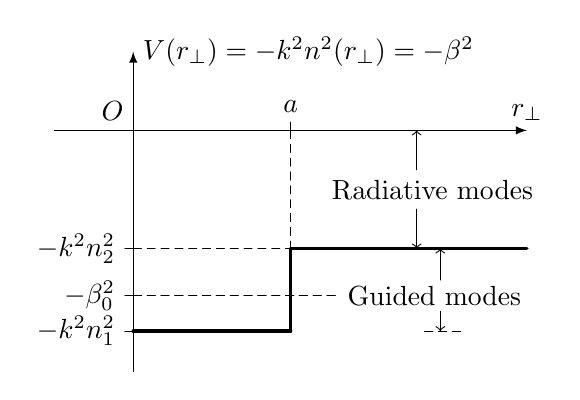
\begin{tikzpicture}[scale=1,cap=round]
% Configurable parameters
\def\k{1.5cm}
\def\eps{1.5*1.7cm}
\def\betasq{1.5*1.4cm}
\def\a{2cm}
\def\maxr{5cm}

% Styles
\tikzstyle{axes}=[arrows={-latex}]
\tikzstyle{auxline}=[densely dashed]
\tikzstyle{important line}=[very thick]

% Coordinates and points.
\coordinate (O) at (0,0);	% Origin.
\coordinate (A) at (\a,0);	% The surface distance to the axis of the fiber.
\coordinate (B) at (0,-\eps);	% -k^2\epsilon at the center of the fiber.
\coordinate (C) at (\a,-\eps);	% -k^2\epsilon on the surface of the fiber.
\coordinate (D) at (0,-\betasq);	% -\beta^2 point at the center of the fiber.
\coordinate (E) at (\a*1.3,-\betasq);	% -\beta^2 point at the end of the maximum r.
\coordinate (F) at (0,-\k);	% -k^2 point at the center of fiber.
\coordinate (G) at (\a,-\k); 	% -k^2 point on the surface of the fiber.
\coordinate (H) at (\maxr,-\k); 	% -k^2 point at the end of r.

% The graphic
 % help grid
% \draw[style=help lines,step=0.5cm] (-2.0,-2.0) grid (2.0,2.0);
  
% Draw axes and marks.
\draw [axes] (-1cm, 0) -- (\maxr,0) node [above] {$r_{\perp}$};
\draw [axes] (0, -1.2*\eps) -- (0, 1.0cm) node [right] {$V(r_{\perp})=-k^2n^2(r_{\perp})=-\beta^2$};
\draw (O) node [above left] {$O$};
\draw[thin] (A) -- (\a,3pt) node[anchor=south] {$a$}; 
\draw (B) -- (-3pt,-\eps) node[anchor=east] {$-k^2n_1^2$};
\draw (D) -- (-3pt,-\betasq) node[anchor=east] {$-\beta_0^2$};
\draw (F) -- (-3pt,-\k) node[anchor=east] {$-k^2n_2^2$};

% Draw potential lines.
\draw[important line] (B) -- (C);
\draw[important line] (C) -- (G);
\draw[important line] (G) -- (H);
\draw[auxline] (D) -- (E) node[right] {Guided modes};
\draw[auxline,very thin] (F) -- (G);
\draw[auxline,very thin] (A) -- (G);

% Other labels and auxlines.
%\draw[<->] (\a*1.25,0) -- (\a*1.25,-\k) node[midway,right] {Scattered modes};
\draw (\a*1.2,-\k/2) node[right] {Radiative modes};
\draw[<-] (\a*1.8,0) -- (\a*1.8,-0.5cm);
\draw[->] (\a*1.8,-1cm) -- (\a*1.8,-\k);
\draw[<-] (\a*1.95,-\k) -- (\a*1.95,-\k-0.4cm);
\draw[->] (\a*1.95,-\k-0.8cm) -- (\a*1.95,-\eps);
\draw[auxline] (\a*1.85,-\eps) -- (\a*2.08,-\eps);
\end{tikzpicture}
}
\caption[Trapping potential analog of the bounded and unbounded modes of a waveguide.]{Bound and unbound states for the nanofiber eigenvalue 
problem. $ \varepsilon(r\!_\perp)=\varepsilon_{f} =n_1^2$ if $ r_\perp < a $; otherwise, $\varepsilon
(r\!_\perp) =1 $. The parameter $ a $ is the radium of the nanofiber.}
\label{Figs/scatteredmode}
\end{figure}

Using the relationship that
\begin{align}
\nabla^2 \!_\perp = \frac{1}{r_{\!\perp}}\pp{}{r\!_\perp}\! \left(r\!_\perp \pp{}{r\!_\perp} \right) + 
\frac{1}{r_\perp^2} \spp{}{\phi},
\end{align}
and the symmetry of the fiber,  we can  separate the mode function by
\begin{align}
\psi(r\!_\perp,\phi)=\mathcal{E}_{z,\beta m}(r\!_\perp)e^{im\phi},
\end{align} 
and hence
\begin{align}
\mathcal{E}_z(r\!_\perp,\phi,z) = \mathcal{E}_{z,\beta m}(r\!_\perp)e^{i(m\phi+\beta z)},
\end{align}
where $ \mathcal{E}_{z,\beta m}(r\!_\perp) $ satisfies the Bessel's equation
\begin{align}
\left[ \spp{}{r\!_\perp}+ \frac{1}{r_{\!\perp}}\pp{}{r\!_\perp}- 
\frac{m^2}{r^2\!_\perp} + (k^2\varepsilon(r\!_\perp)-\beta^2) \right] 
\mathcal{E}_{z,\beta m}(r\!\!_\perp)=0
\end{align}
with 
\begin{align}
\varepsilon(r\!\!_\perp) = 
\begin{cases}
1, & r\!_\perp>a\\
\varepsilon_f, & r\!_\perp\leq a.
\end{cases}
\end{align}
The general solution for $ \mathcal{E}_{z,\beta m}(r\!\!_\perp) $ can be given in three cases 
corresponding to different 
boundary conditions
\begin{align}
\mathcal{E}_{z,\beta m}(r\!\!_\perp) = \begin{cases}
AJ_m(qr\!\!_\perp) + B Y_m(qr\!_\perp)&\rightarrow J_m(\theta)\sim \cos\theta,\, Y_m(\theta)\sim 
\sin\theta.\\
CI_m(qr\!_\perp) + DK_m(qr\!_\perp) & \rightarrow I_m(\theta) \sim e^\theta,\, K_m(\theta) \sim 
e^{-\theta}.\\
EH_m^{(\!1\!)}(qr\!_\perp) \!+\! FH_m^{(\!2\!)}(qr\!_\perp ) & \rightarrow H_m^{(\!1\!)} (\theta) \! \sim \! 
e^{i\theta},\, 
H_m^{(\!2\!)}(\theta)\!\sim\! e^{\!-i\theta}.
\end{cases}
\end{align}
The positive parameter $ 1/q $ is the characteristic decay length corresponding to $ 1/h_{11} $ and $ 
1/q_{11} $ 
in the $\text{HE}_{11}$ mode expression. Using the symmetric and convergent condition at $ 
r\!_\perp=0\,\text{and}\, \infty $, as for bound modes, for example, if $k< \beta\leq 
k\sqrt{\varepsilon_f}$,
\begin{align}
\left\{
 \begin{array}{lcll}
	r\!_\perp \leq a, & \mathcal{E}_{z,\beta m}(r\!_\perp )\!=\! AJ_m(h r\!_\perp), & h \!=\! 
	\sqrt{k^2\varepsilon_f-\beta^2}\! >\! 0;\\
	r\!_\perp > a, & \mathcal{E}_{z,\beta m}(r\!_\perp )\!=\!DK_m(q r\!_\perp), & q\!=\! 
	\sqrt{\beta^2-k^2}>0.
 \end{array}\right.
\end{align}
Both $ \beta $ and $ h $ are discrete for bound modes. 
For scattered modes, $ 0\leq \beta< k $, similarly, 
\begin{align}
\left\{
 \begin{array}{lcll}
	r\!_\perp \leq a, & \mathcal{E}_{z,\beta m}(r\!_\perp )\!=\! AJ_m(h r\!_\perp), & h \!=\! 
	\sqrt{k^2\varepsilon_f-\beta^2}\! >\! 0;\\
	r\!_\perp > a, & \mathcal{E}_{z,\beta m}(r\!_\perp )\!=\!EH_m^{(\!1\!)}(p r\!_\perp\!), & p\!\!=\!\! 
	\sqrt{k^2-\beta^2}>0.
 \end{array}\right.
\end{align}
Both $ \beta $ and $ p $ are continuous. 
%\textcolor{red}{(Double check the general solutions and the consistence with Equ.~\ref{ET0Rexpand}.)}
%Notice that Ref.\cite{Snyder1983} used $ J_m(hr\!_\perp)\cos m\phi $ and $ 
%(J_m(pr\!_\perp)+CH_m^{(\!1\!)})\cos m\phi $ as the basis for the general solution of $ e $ and $ o $ 
%light 
%of the radiation modes, and summed them up. They are equivalent to the solution here.  

If $ \beta $ is a pure imaginary number, the field will have an exponential decay amplitude on $ z $-direction, and will spread the energy away from the fiber axis. Reference~\cite{Snyder1983} denotes the modes with pure imaginary $ \beta $ as evanescent modes. If $ \beta $ has both real and imaginary parts, the modes are denoted as leaky modes, which are combinations of radiation modes and evanescent modes. Except for the case that the incident light is highly directed at the complementary critical angle $ \theta_c $ of geometric optics, only the radiation modes part can propagate for a long distance along the fiber axis. In our nanofiber system, we only consider the bound and radiation modes. The ranges of some waveguide parameters are given in Table~\ref{tab:fiberparameters}. 
In the table, we have defined the normalized wave number\cite{Snyder1983}, or 
$V$-number\index{$V$-number} 
of a fiber as $V  = 
k_f a \mathrm{NA}$.  Here $k_f=\frac{2\pi}{\lambda}$, is the free space wave number, $a$ is the radius 
of the core of the fiber, and $\mathrm{NA}$ is the numerical aperture\index{numerical aperture} of 
the fiber, $\mathrm{NA} = 
(n_{core}^2 - n_{cladding}^2)^{1/2} = n_{core}(2\Delta)^{1/2}$, with profile height 
parameter\index{profile height parameter} 
$\Delta =\frac{1}{2}(1-n_{cladding}^2/n_{core}^2)\approx (n_{core}-n_{cladding})/n_{core}$.  For 
different modes labeled with $ j $, we always have $V_j^2=a^2(h_j^2+q_j^2)$ and $ \lambda\beta_j/2\pi $ is a mode invariance.  The TE and TM modes have non-vanishing cut-off 
frequencies, as $ a\rightarrow 0 $.  The cutoff frequency is found from $V = a\omega (\Delta)^{1/2}/c =2.405$ for silicon fiber.  
Only the lowest HE mode, $\mathrm{HE}_{11}$, has no cutoff frequency as $ a\rightarrow 0 $.  For $0 < V < 2.405$, which is the case of the nanofiber we are studying, it is the only mode that propagates in the 
fiber. For fixed $ \varepsilon_f $, in the range that $ 0\leq \beta \leq 
k\sqrt{\varepsilon_f} $, we can distinguish the radiative and bound mode as follows:
\begin{align}
\begin{cases}
0\leq \beta < k, &\rightarrow \textit{unbounded radiative modes;}\\
k< \beta \leq k \sqrt{\varepsilon_f}, &\rightarrow \exists a,\, \textit{HE}_{11}\, \textit{is the only 
bound mode.}
\end{cases}
\end{align}


\begin{minipage}{0.97\textwidth}
\centering
\captionof{table}{Ranges of fiber parameters for different modes. } \label{tab:fiberparameters} 
\begin{tabular}{|l|c|c|c|}
\hline  & $\beta$ & $h$ & $p$ \\ 
\hline Bound modes & $k<\beta_j \leq k\sqrt{\varepsilon_f} $ & $ 0\leq h_j<V/a $ & $ p^r_j=0,\, p^i_j>0 $ \\ 
\hline Radiation modes & $0\leq \beta<k$ & $V/a < h\leq k\sqrt{\varepsilon_f}$ & $0<p\leq k $\\ 
\hline Evanescent modes & $ \beta^r=0,\, \beta^i>0 $ & $ k\sqrt{\varepsilon_f} < h $ & $ k<p $ \\ 
\hline 
\end{tabular} 
\par
\bigskip
%The caption:
Superscripts $ r $ and $ i $ denote real and imaginary parts. Subscripts $ j $ denotes the discrete indeces for bound modes. Adapted from Ref.~\cite{Snyder1983} P.P.516 Table 25-1. This can also be understood in geometric optics as shown in Fig.(\ref{fig:Fibermodes}).
\end{minipage}
\bigskip

\begin{figure}
\centering\makebox[\textwidth]{
\begin{tikzpicture}[scale=1,cap=round]
% Configurable parameters
\def\fiberrad{1cm}	% Radius of the nanofiber.
\def\comprad{0.45cm}	% Compressed radius of the nanofiber in the view angle.
\def\fiberleftx{0}	% The x-coordiante of the center of the left surface of the fiber.
\def\fiberlefty{0}	% The y-coordiante of the center of the left surface of the fiber.
\def\fiberlength{6.6cm} % The length of the fiber.

% Styles
\tikzstyle{axes}=[arrows={-latex}]
\tikzstyle{auxline}=[densely dashed]
\tikzstyle{important line}=[thick]
\tikzstyle{dot}=[circle,inner sep=1pt,fill,label={#1},name=#1]

% Coordinates and points.
\coordinate (O) at (0,0);	% Origin.
\coordinate (LO) at (\fiberleftx,\fiberlefty); % Center of the left-side surface of the nanofiber.
\coordinate (RO) at (\fiberleftx+\fiberlength,\fiberlefty); % Center of the right-side surface
\coordinate (A) at ({\fiberleftx},{\fiberlefty+\fiberrad});	% Top-left point of the nanofiber.
\coordinate (B) at ({\fiberleftx+\fiberlength},{\fiberlefty+\fiberrad});	% Top-right point of the nanofiber.
\coordinate (C) at ({\fiberleftx+\fiberlength},{\fiberlefty-\fiberrad});	% Bottom-right point of the fiber.
\coordinate (D) at ({\fiberleftx},{\fiberlefty-\fiberrad});	% Bottom-left point of the nanofiber.

% The graph.
% help grid
% \draw[style=help lines,step=0.5cm] (-2.0,-2.0) grid (2.0,2.0);

% Draw the fiber.
\begin{scope} 
    % Outer edge.
    %\fill[left color=purple!50!black,right color=purple!50!black,middle 
%color=purple!50,shading=axis,opacity=0.25] (A) -- (B) arc (90:270:{\comprad} and {\fiberrad}) -- (D) arc 
%(270:90:{\comprad} and {\fiberrad});
    % Right-side surface.
    %\fill[top color=purple!90!,bottom color=purple!2,middle color=purple!30,shading=axis,opacity=0.25] 
%(RO) circle [x radius={\comprad}, y radius = {\fiberrad}];
    % Draw lines of all edges.
    \draw (A) -- (B);
    \draw  (RO) circle [x radius = {\comprad}, y radius =  {\fiberrad}];
    \draw (C) -- (D) arc (270:90:{\comprad} and {\fiberrad}); 
    \draw[densely dashed] (A) arc (90:-90:{\comprad} and {\fiberrad});
\end{scope}

% Draw the guide mode wave vector and propagation lines.
% First part of the ray: up-solid line.
\draw[red] (O)--(2.0*\fiberrad,\fiberrad);
%\draw[red,decoration={ markings,  % This schema allows for fine-tuning the arrows.
%      mark=at position 0.5 with {\arrow{latex'}}, 
%      mark=at position 0.82 with {\arrow{latex'}}},postaction={decorate}] (O) -- (2.0*\fiberrad,\fiberrad)-- (6.0*\fiberrad,-\fiberrad);
% The penetration part of ray: dashed line.
\draw[red,densely dotted] (2.0*\fiberrad,\fiberrad) -- (2.3*\fiberrad,1.1732*\fiberrad) -- (2.6*\fiberrad,\fiberrad);
% The reflected part: solid downarrow.
\draw[red,decoration={ markings,  % This schema allows for fine-tuning the arrows.
      mark=at position 0.2 with {\arrow{latex'}}, 
      mark=at position 0.6 with {\arrow{latex'}}},postaction={decorate}] (2.6*\fiberrad,\fiberrad)-- (6.6*\fiberrad,-\fiberrad);
% The ruler part.
\draw[important line,-latex'] (O) --(27:1) node[below,xshift=8,yshift=5] {$ \vec{k} $};
\draw[auxline] (27:1) -- ({cos(27)},-1.5)  node [below] {$\beta_0$};

% Draw radiation modes.
% Radiation ray 1:
\draw[blue,decoration={ markings,  % This schema allows for fine-tuning the arrows. 
      mark=at position 0.95 with {\arrow{latex'}}},postaction={decorate}] (O) -- (0.5,\fiberrad) -- (1.5,\fiberrad*1.1);
\draw[-latex'] (O)--(63.5:1);
\draw[auxline] (63.5:1) -- ({cos(63.5)},-2);
% Radiation ray 2:
\draw[blue,decoration={ markings,  % This schema allows for fine-tuning the arrows. 
      mark=at position 0.95 with {\arrow{latex'}}},postaction={decorate}] (O) -- (0.4,\fiberrad) -- (1.4,\fiberrad*1.4);
\draw[-latex'] (O)--(68.5:1);
\draw[auxline] (68.5:1) -- ({cos(68.5)},-2);
% Radiation ray 3:
\draw[blue,decoration={ markings,  % This schema allows for fine-tuning the arrows. 
      mark=at position 0.95 with {\arrow{latex'}}},postaction={decorate}] (O) -- (0.25,\fiberrad) -- (0.9,\fiberrad*1.9);
\draw[-latex'] (O)--(76:1);
\draw[auxline] (76:1) -- ({cos(76)},-2);
% Radiation ray 3:
\draw[blue,decoration={ markings,  % This schema allows for fine-tuning the arrows. 
      mark=at position 0.95 with {\arrow{latex'}}},postaction={decorate}] (O)-- (0,2*\fiberrad);
\draw[-latex'] (O) -- (0,\fiberrad);
% Draw dots inbetween.
\draw[dotted] ([shift=(26:1)] 0.2,1.0*\fiberrad) arc (26:45:1);
\draw[dotted] ([shift=(60:1)] 0.1,1.0*\fiberrad) arc (60:89:1);

% Labels and denotes.
\draw (O) node[dot] {};
\draw (O) node[left] {O};
\draw[auxline,-latex] (O) -- (\fiberlength*1.0,0) node [above] {$ z $};	% Z axis line.
\draw[auxline] (0,\fiberrad) -- (0,-2);
\draw[important line,-latex] (0,-2) node[left] {$ 0 $}--(2.5,-2) node[right] {$ k_z $};% kz axis.
\draw (0,-2) -- (0,-2.08);
\draw (0.5,-2) -- (0.5,-2.08) node [anchor=north] {$k_0$};
\draw ({cos(27)},-2) -- ({cos(27)},-2.08);
\draw (1.1,-2) -- (1.1,-2.08) node [below right,xshift=-5] {$k_0n_1$};
\draw (3.35,-0.5) node[red] {Guided modes};	% Guided modes label.
\draw (2.7,1.7*\fiberrad) node[blue] {Radiative modes};	% Radiative modes label.
\end{tikzpicture}
}
\caption{Fiber modes classified through the $ z $-component of the wave vector.}
\label{fig:Fibermodes}
\end{figure}

Due to the symmetry of equations, we also have
\begin{align}
\mathcal{B}_z(r\!_\perp,\phi,z) = \mathcal{B}_{z,\beta m}(r\!_\perp)e^{i(m\phi+\beta z)},
\end{align}
where $  \mathcal{B}_{z,\beta m}(r\!_\perp) $ satisfies the same Bessel's equation as above. 

Next, we consider the case that an atom--which can be treated as an electric dipole in the regime we are interested in--is placed next to the 
nanofiber. Equ.~\eqref{Esrt0} can be rewritten as 
\begin{align}
\boldsymbol{\mathcal{E}}(\br) &= \boldsymbol{\mathcal{E}}_{source}(\br) + 
\boldsymbol{\mathcal{E}}_{ref}(\br)+\boldsymbol{\mathcal{E}}_{tran}(\br)\\
&=
	\begin{cases}
	  \boldsymbol{\mathcal{E}}_{dipole} (\br)+ \boldsymbol{\mathcal{E}}_{ref}(\br) & r\!_\perp \geq a,\\
	  \boldsymbol{\mathcal{E}}_{tran}(\br) & r\!_\perp<a.
	\end{cases} \\
&=
	\begin{cases}
		  \boldsymbol{\mathcal{E}}^{(0)} (\br)+ \boldsymbol{\mathcal{E}}^{(R)}(\br) & r\!_\perp \geq a,\\
		  \boldsymbol{\mathcal{E}}^{(T)}(\br) & r\!_\perp<a.
		\end{cases} \label{Etotalfiber}
\end{align}


For longitudinal components of the electrical and magnetic fields we expand them as follows
\begin{subequations}\label{ET0Rexpand}
\begin{align}
\mathcal{E}^{(T)}_z &= \sum_{m=-\infty}^\infty \int \mathrm{d}\beta e^{im(\phi-\phi') + i\beta (z-z')} \mathcal{E}^{(T)}_{z,m\beta}(r\!_\perp)\\
&= \sum_{m=-\infty}^\infty \int \mathrm{d}\beta e^{im(\phi-\phi') + i\beta (z-z')} c_{m\beta} J_m (hr\!_\perp),\\
% + B_{m\beta} Y_m(hr\!_\perp)\right],\\
\mathcal{E}^{(0)}_{z} &= \sum_{m=-\infty}^\infty \int \mathrm{d}\beta e^{im(\phi-\phi') + i\beta (z-z')} \mathcal{E}^{(0)}_{z,m\beta}(r\!_\perp)\\
\mathcal{E}^{(R)}_z &= \sum_{m=-\infty}^\infty \int \mathrm{d}\beta e^{im(\phi-\phi') + i\beta (z-z')} \mathcal{E}^{(R)}_{z,m\beta}(r\!_\perp)\\
&= \sum_{m=-\infty}^\infty \int \mathrm{d}\beta e^{im(\phi-\phi') + i\beta (z-z')} a_{m\beta} H_m^{(1)} (pr\!_\perp),
\end{align}
\end{subequations}
\begin{subequations}\label{BT0Rexpand}
\begin{align}
\mathcal{B}^{(T)}_z &= \sum_{m=-\infty}^\infty \int \mathrm{d}\beta e^{im(\phi-\phi') + i\beta (z-z')} \mathcal{B}^{(T)}_{z,m\beta}(r\!_\perp)\\
&= \sum_{m=-\infty}^\infty \int \mathrm{d}\beta e^{im(\phi-\phi') + i\beta (z-z')} d_{m\beta} J_m (hr\!_\perp),\\
% + E_{m\beta} Y_m(hr\!_\perp)\right],\\
\mathcal{B}^{(0)}_{z} &= \sum_{m=-\infty}^\infty \int \mathrm{d}\beta e^{im(\phi-\phi') + i\beta (z-z')} \mathcal{B}^{(0)}_{z,m\beta}(r\!_\perp)\\
\mathcal{B}^{(R)}_z &= \sum_{m=-\infty}^\infty \int \mathrm{d}\beta e^{im(\phi-\phi') + i\beta (z-z')} \mathcal{B}^{(R)}_{z,m\beta}(r\!_\perp)\\
&= \sum_{m=-\infty}^\infty \int \mathrm{d}\beta e^{im(\phi-\phi') + i\beta (z-z')} b_{m\beta} H_m^{(1)} (pr\!_\perp),
\end{align}
\end{subequations}
where the subscripts indicate the field components of reflection ($R$), dipole oscillation in free space ($0$) and transmission ($ T $). Notice that we have chosen $ m=\pm 1 $, as the nanofiber can only support HE$_{11}$ modes. 
The $ r\!_\perp $ and $ \phi $ components of the fields can be obtained using Equ.~\eqref{EHzgauss} and $ \mathcal{B}=\mathcal{H} $ in Gauss units for given $ m $. Also notice, in the nanofiber case we are studying, we can define $ z'=0 $ and $ \phi'=0 $, and hence the factor $ e^{im(\phi-\phi') + i\beta (z-z')} $ in the equations above becomes $ e^{im\phi + i\beta z} $. That is what Klimov and others have used in their paper.

The free space dipole emits an electromagnetic field described by
\begin{align}
\mathcal{A} &= -ik \mathbf{d}_0 \frac{e^{ik|\br-\br'|}}{|\br-\br'|},
\end{align}
\begin{align}
\mathcal{B}^{(0)} &= \nabla\times \mathcal{A}\nonumber \\
&=-ik\nabla(\frac{e^{ik|\br-\br'|}}{|\br-\br'|})\times\mathbf{d}_0=-ik\nabla G_0(\br,\br')\times\mathbf{d}_0\nonumber\\
&=\quad\left[\frac{d_z}{r\!_\perp}\pp{G_0(\br,\br')}{\phi}\!-\! d_\phi\pp{G_0(\br,\br')}{z}\right]\mathbf{e}_{r\!_{\perp}}\nonumber\\
&\quad+\left[d_{r\!_\perp}\pp{G_0(\br,\br')}{z}\!-\!d_z\pp{G_0(\br,\br')}{r\!_\perp} \right]\mathbf{e}_\phi \nonumber\\
&\quad+ \left[d_\phi\pp{G_0(\br,\br')}{r\!_\perp}\!-\! \frac{d_{r\!_\perp}}{r\!_\perp}\pp{G_0(\br,\br')}{\phi} \right]\mathbf{e}_z\\
&=\mathcal{B}^{(0)}_{r\!_\perp}\mathbf{e}_{r\!_{\perp}} +\mathcal{B}^{(0)}_\phi\mathbf{e}_\phi + \mathcal{B}^{(0)}_z\mathbf{e}_z,\\
\mathcal{E}^{(0)} &= \frac{i}{k} \nabla\times \mathcal{H}^{(0)}=\frac{i}{k}\nabla\times \mathcal{B}^{(0)}\nonumber\\
&=\frac{i}{k}(\frac{1}{r\!_\perp}\!\pp{\mathcal{B}^{(\!0\!)}_z}{\phi}\!-\! \pp{\mathcal{B}^{(\!0\!)}_\phi}{z})\mathbf{e}_{r\!_{\perp}} \!\!+\! \frac{i}{k}(\!\pp{\mathcal{B}^{(\!0\!)}_{r\!_\perp}}{z} \!-\! \pp{\mathcal{B}^{(\!0\!)}_z}{r\!_\perp})\mathbf{e}_\phi \!\!+\! \frac{i}{r\!_\perp\! k} (\!\pp{(\! r\!_\perp \mathcal{B}^{(\!0\!)}_\phi)}{r\!_\perp} \!\!-\!\! \pp{\mathcal{B}^{(\!0\!)}_{r\!_\perp}}{\phi}\! )\mathbf{e}_z\\
&=\mathcal{E}^{(0)}_{r\!_\perp}\mathbf{e}_{r\!_{\perp}} +\mathcal{E}^{(0)}_\phi\mathbf{e}_\phi + \mathcal{E}^{(0)}_z\mathbf{e}_z,
\end{align}
or, by Equ.~\eqref{EGd}. Here, $ \mathbf{d}_0 $ is the dipole momentum in vacuum. We denote $d_{r\!_\perp},\, d_\phi$ and $d_z$ as the cylindrical components of the dipole momentum at arbitrary observation point ${\rm {\bf r}}=\left( {r\!_\perp ,\phi ,z}\right) $; while we use $d^0_{r\!_\perp}$, $d^0_\phi$ and $d^0_z$ to indicate the cylindrical components of the dipole momentum at the dipole position ${\rm 
{\bf {r}^{\prime }}}=\left( {{r\!_\perp }^{\prime },{\phi }^{\prime },{z}^{\prime }}\right) $. As shown in Fig.(\ref{fig:dipolemomentumtransmission}) on page~\pageref{fig:dipolemomentumtransmission}, we defined the vector from the center of the nanofiber's core pointing to the atom position as $x$-axis, and the rotating symmetric axis of the nanofiber as the $z$-axis. The relationships between the dipole momentum components at $\mathbf{r}$ and $\mathbf{r}'$ can be given by
\begin{align}
d_{r\!_\perp}\! &= \cos(\phi\!-\!\phi')d^0_{r\!_\perp}\!\!+\!\sin(\phi\!-\!\phi')d^0_\phi=\frac{1}{\sqrt{2}}\left(-e^{-i(\phi\!-\!\phi')}d_++e^{i(\phi\!-\!\phi')}d_- \right),\\
d_\phi &=\cos(\phi\!-\!\phi')d^0_\phi\!-\!\sin(\phi\!-\!\phi')d^0_{r\!_\perp}=\frac{i}{\sqrt{2}}\left(e^{-i(\phi\!-\!\phi')}d_++e^{i(\phi\!-\!\phi')}d_- \right),\\
d_z &= d^0_z,
\end{align}
where I have defined the position-independent reduced dipole vector components
\begin{align}
d_\pm \equiv \mp \frac{1}{\sqrt{2}}(d^0_{r\!_\perp}\pm id^0_{\phi}).
\end{align}
The terms associated with $d_\pm$ in the dipole moment formula lower or raise the mode index by $1$. Notice that we have used $\phi\!-\!\phi'$ as the projected angle between $\mathbf{r}$ and $\mathbf{r}'$ to make the relationship work in general. 

\begin{figure}
\centering\makebox[\textwidth]{
\begin{tikzpicture}[scale=2,cap=round]
% Local definitions
  \def\AngleAtr{60}	% angle of r w.r.t x-axis
  \def\AngleOfd{30}	% angle of d w.r.t. x-axis
  \def\LenOfd{1cm} % length of the dipole momentum vector
  \def\drp{0.8660cm}	% drp at r'
  \def\dphi{0.5cm}	% dphi at r'
  \def\drpr{0.8660}	% drp at r
  \def\dphir{-0.5}	% dphi at r
  \def\Angledrp{\AngleAtr}	% angle of drp w.r.t. x-axis
  \def\Angledphi{150}
  
  \coordinate (O) at (0,0);		% origin
  \coordinate (R) at (2.0cm,0); % position of the dipole at r'
  \coordinate (r) at (\AngleAtr:1.3cm);	% position of observation point

  % Colors
  \colorlet{anglecolor}{green!50!black}
  \colorlet{rvectorcolor}{red}
  \colorlet{assisvectorcolor}{orange!80!black}
  \colorlet{momentumcolor}{blue}

  % Styles
  \tikzstyle{axes}=[]
  \tikzstyle{important line}=[very thick]
  \tikzstyle{information text}=[rounded corners,fill=red!10,inner sep=1ex]

  % The graphic
  % help grid
  %\draw[style=help lines,step=0.5cm] (-2.0,-2.0) grid (2.0,2.0);
  
  % circle for the nanofiber scope
  \draw (0,0) circle (1cm); 
  \draw[<->] (0,0) --node[left=1mm] {$a$} (225:1cm) ;
  \draw (-30:1.8cm) node {\text{nanofiber intersection}};
  % coordinates
  \begin{scope}[style=axes]
    \draw[->] (-1.3cm,0) -- (3.0cm,0) node[right] {$\mathbf{x}$};
    \draw[->] (0,-1.3cm) -- (0,2.0cm) node[above] {$\mathbf{y}$};
    \draw (-1mm,1mm) node {$O$};
  \end{scope}
  
  % angle and position vector for r
  \filldraw[fill=green!20,draw=anglecolor] (0,0) -- (3mm,0pt) arc(0:\AngleAtr:3mm);
    \draw (20:6mm) node[anglecolor] {$\phi\!-\! \phi'$};
  \draw[->,style=important line,rvectorcolor] (O) -- (r) node[left=1.5mm] {$\mathbf{r}$};
  % arc between two decomposition approaches
  \filldraw[fill=green!20,draw=anglecolor] (r.center)--($(r.center)+(2mm,0)$) arc (0:\AngleAtr:2mm);
  \draw ($(r.center)+(10:4.4mm)$) node[anglecolor] {$\phi\!-\! \phi'$};
  % dipole momentum vector at r
  \draw[->,style=important line,momentumcolor] (r) -- +(\AngleOfd:\LenOfd) node[right] {$\mathbf{d}_0$};
  
  % d vector components at r
  \draw[->,dashed,thick,assisvectorcolor] (r) -- +(0:\drp) node[right] {$d^0_{r\!_\perp}$};
  \draw[style=dotted,assisvectorcolor] ($(r.center)+(0:\drp)$) -- ($(r.center)+(\AngleOfd:\LenOfd)$);
  \draw[->,dashed,thick,assisvectorcolor] (r) -- +(90:\dphi) node[left] {$d^0_\phi$};
  \draw[style=dotted,assisvectorcolor] ($(r.center)+(90:\dphi)$) -- ($(r.center)+(\AngleOfd:\LenOfd)$);
  \draw[->,thick,dashed,anglecolor] (r) -- +(\Angledrp:\drpr) node[yshift=8mm,xshift=1.8cm,anchor=north] {$d_{r\!_\perp}\!=\frac{1}{\sqrt{2}}\left(-e^{-i(\phi\!-\!\phi')}d_++e^{i(\phi\!-\!\phi')}d_- \right)$};
  \draw[style=dotted,anglecolor] ($(r.center)+(\Angledrp:\drpr)$) -- ($(r.center)+(\AngleOfd:\LenOfd)$);
  \draw[->,thick,dashed,anglecolor] (r) -- +(\Angledphi:\dphir) node[right] {$d_\phi=\frac{i}{\sqrt{2}}\left(e^{-i(\phi\!-\!\phi')}d_++e^{i(\phi\!-\!\phi')}d_- \right)$};
  \draw[style=dotted,anglecolor] ($(r.center)+(\Angledphi:\dphir)$) -- ($(r.center)+(\AngleOfd:\LenOfd)$);
  \draw [fill=blue] (r) circle (0.2mm) node {}; % starting point at r
   
  % dipole momentum vector for r'
  \draw[->,style=important line,rvectorcolor] (O) -- (R) node[below=1mm] {$\mathbf{r}'$};
  \draw[->,style=important line,momentumcolor] (R) -- +(\AngleOfd:\LenOfd) node[right] {$\mathbf{d}_0$};
  \draw[->,very thick,dashed,assisvectorcolor] (R) -- +(0:\drp) node[below] {$d^0_{r\!_\perp}$};
  \draw[style=dotted,assisvectorcolor] ($(R.center)+(0:\drp)$) -- ($(R.center)+(\AngleOfd:\LenOfd)$);
  \draw[->,thick,dashed,assisvectorcolor] (R) -- +(90:\dphi) node[left] {$d^0_\phi$};
  \draw[style=dotted,assisvectorcolor] ($(R.center)+(90:\dphi)$) -- ($(R.center)+(\AngleOfd:\LenOfd)$);
  \draw [fill=blue] (R) circle (0.2mm) node {}; % starting point at r'
\end{tikzpicture}}
\caption{Dipole momentum decompositions in the $xy$-plane.}
\label{fig:dipolemomentumtransmission}
\end{figure}

Using the expansion of the free-space scalar Green function (Equ.~\eqref{scalarG}) for the space $ \left(r\!_\perp <r_\perp ^{\prime}\right) $ that 
\begin{align}
\frac{G_0(\br,\br')}{k^2} &={\frac{{e^{ik{\left| {{\rm {\bf r}}-{\rm {\bf {r}^{\prime }}}}\right| }}}}{{{%
\left| {{\rm {\bf r}}-{\rm {\bf {r}^{\prime }}}}\right| }}}}\nonumber\\
&={\frac{{i}}{{2}}%
}{\sum\limits_{m=-\infty }^{\infty } {{\oint\limits_{C_{1}}{\mathrm{d}\beta \;e^{im\left( {\phi -{\phi }%
^{\prime }}\right) +i\beta \left( {z-{z}^{\prime }}\right) }J_{m}\left( {pr\!_\perp
}\right) H_{m}^{\left( {1}\right) }\left( pr_\perp ^{\prime
}\right) }}}},
\end{align}
and for $ \left(r\!_\perp >r_\perp ^{\prime}\right) $
\begin{align}
\frac{G_0(\br,\br')}{k^2} &={\frac{{e^{ik{\left| {{\rm {\bf r}}-{\rm {\bf {r}^{\prime }}}}\right| }}}}{{{%
\left| {{\rm {\bf r}}-{\rm {\bf {r}^{\prime }}}}\right| }}}}\nonumber\\
&={\frac{{i}}{{2}}%
}{\sum\limits_{m=-\infty }^{\infty } {{\oint\limits_{C_{1}}{\mathrm{d}\beta \;e^{im\left( {\phi -{\phi }%
^{\prime }}\right) +i\beta \left( {z-{z}^{\prime }}\right) }J_{m}\left( {pr\!_\perp^{\prime} }\right) H_{m}^{\left( {1}\right) }\left( pr_\perp \right) }}}},
\end{align}
one can obtain the free space dipole radiation field components in Equ.~\eqref{ET0Rexpand} and~\eqref{BT0Rexpand}. The contour $ C_1 $ and field components can be found in Ref.~\cite{Klimov2004}. ~\footnote{Similarly, the decomposition of a plane wave function can be found in Appendix~\ref{Ch:PlanewaveDecomposition}}.

The free radiation field components associated with the $ e^{im\phi+i\beta z} $ term (the $m$-th mode components) for the $r\!_\perp<r'\!_\perp$ region can be given by
\begin{align}
\mathcal{B}_{z,m\beta}^{(0)} &= \frac{ikp}{2\sqrt{2}}J_m(pr\!_\perp)\left[ d_{+} H_{m+1}^{(1)}(pr'\!\!_\perp) \!-\! d_- H_{m-1}^{(1)}(pr'\!_\perp) \right],\\
\mathcal{B}_{\phi,m\beta}^{(0)} &= \frac{ik}{2}\left[ \frac{\beta d_{-}}{\sqrt{2}} J_{m-1}\left( pr\!_\perp \right)H_{m-1}^{(1)}\left( {pr\!_\perp^{\prime} }\right) -\frac{\beta d_+}{\sqrt{2}} J_{m+1}\left( pr\!_\perp \right)H_{m+1}^{(1)}\left( {pr\!_\perp^{\prime} }\right)\right. \nonumber\\ 
&\qquad\quad \left. + \frac{ipd^0_z}{2}\left(J_{m-1}(pr\!_\perp)-J_{m+1}(pr\!_\perp) \right)H_m^{(1)}(pr\!_\perp^{\prime}) \right],\\
\mathcal{B}_{r\!_\perp, m\beta}^{(0)} &= \frac{k}{2}\left[\frac{i m d^0_z}{r\!_\perp} J_m\left( pr\!_\perp \right) H_m^{(1)}\left( {pr\!_\perp^{\prime} }\right) \right. \nonumber\\
&\qquad \left. +\frac{\beta d_+}{\sqrt{2}} J_{m\!+\!1}(pr\!_\perp) H_{m\!+\! 1}^{(1)}(pr\!_\perp^{\prime}) \!+\! \frac{\beta d_-}{\sqrt{2}} J_{m\!-\! 1}(pr\!_\perp)H_{m\!-\!1}^{(1)}(pr\!_\perp^{\prime})   \right],\\
\mathcal{E}_{z,m\beta}^{(0)} 
&= \frac{p}{2}J_{m}\left( pr\!_\perp \right)\left[  id^0_z p H_m^{(1)}\left( {pr\!_\perp^{\prime} }\right) \phantom{\frac{d^0_z}{\sqrt{2}}} \right. \nonumber\\
&\qquad\qquad\qquad \left. + \frac{\beta d_{+}}{\sqrt{2}} H_{m+1}^{(1)}\left( {pr\!_\perp^{\prime} }\right) +\frac{\beta d_-}{\sqrt{2}} H_{m-1}^{(1)}\left( {pr\!_\perp^{\prime} }\right) \right], \\
\mathcal{E}_{\phi,m\beta}^{(0)} 
&= -\frac{im\beta d^0_z}{2r\!_\perp} J_{m}\left( pr\!_\perp \right) H_m^{(1)}\left( {pr\!_\perp^{\prime} }\right) \nonumber\\
&\quad+\frac{d_+}{2\sqrt{2}} \left[ \frac{mp}{r\!_\perp}J_{m}\left( pr\!_\perp \right)-k^2 J_{m+1}\left( pr\!_\perp \right)\right] H_{m+1}^{(1)}\left( {pr\!_\perp^{\prime} }\right) \nonumber\\
&\quad+ \frac{d_-}{2\sqrt{2}}\left[\frac{mp}{r\!_\perp}J_m\!\left( pr_\perp \right)-k^2J_{m-1}\!\left( pr_\perp \right) \right] H_{m-1}^{(1)}\!\left( {pr\!_\perp^{\prime} }\right),\\
\mathcal{E}_{r\!_\perp,m\beta}^{(0)} 
&= \frac{\beta pd^0_z}{4}\left[ J_{m+1}\!\left( pr\!_\perp \right)-J_{m-1}\!\left( pr_\perp \right)\right] H_m^{(1)}\left( {pr\!_\perp^{\prime} }\right)\nonumber\\ 
&\quad -\frac{d_+}{2\sqrt{2}}\left[ i\beta^2J_{m+1}\!\left( pr_\perp \right) +\frac{imp}{r\!_\perp}J_m\!\left( pr_\perp \right)\right] H_{m+1}^{(1)}\!\left( {pr\!_\perp^{\prime} }\right)\nonumber\\
&\quad + \frac{d_-}{2\sqrt{2}}\left[ i\beta^2J_{m-1}\!\left( pr_\perp \right) +\frac{imp}{r\!_\perp}J_m\!\left( pr_\perp \right)\right] H_{m-1}^{(1)}\!\left( {pr\!_\perp^{\prime} }\right).
\end{align}
More details on deriving the E-field components can be found in \textit{Derivation of free-space E-field components.pdf}. Some properties of Bessel functions are used in deriving these expressions (see appendix). 

By exchanging $J_m$ and $H_m^{(1)}$ functions, one can also obtain the field components that the reference~\cite{Klimov2004} did not include for the case of $ r\!_\perp>r'\!_\perp $. The magnetic and electrical fields components for $ \br\!_\perp>\br'\!_\perp $ are 
\begin{align}
\mathcal{B}_{z,m\beta}^{(0)} &= \frac{ikp}{2\sqrt{2}}H^{(1)}_m(pr\!_\perp)\left[ d_{+} J_{m+1}(pr'\!\!_\perp) \!-\! d_- J_{m-1}(pr'\!_\perp) \right],\\
\mathcal{B}_{\phi,m\beta}^{(0)} &= \frac{ik}{2}\left[ \frac{\beta d_{-}}{\sqrt{2}} H^{(1)}_{m-1}\left( pr\!_\perp \right)J_{m-1}\left( {pr\!_\perp^{\prime} }\right) -\frac{\beta d_+}{\sqrt{2}} H^{(1)}_{m+1}\left( pr\!_\perp \right)J_{m+1}\left( {pr\!_\perp^{\prime} }\right)\right. \nonumber\\ 
&\qquad\quad \left. + \frac{ipd^0_z}{2}\left(H^{(1)}_{m-1}(pr\!_\perp)-H^{(1)}_{m+1}(pr\!_\perp) \right)J_m(pr\!_\perp^{\prime}) \right],\\
\mathcal{B}_{r\!_\perp, m\beta}^{(0)} &= \frac{k}{2}\left[\frac{i m d^0_z}{r\!_\perp} H^{(1)}_m\left( pr\!_\perp \right) J_m\left( {pr\!_\perp^{\prime} }\right) \right. \nonumber\\
&\qquad \left. +\frac{\beta d_+}{\sqrt{2}} H^{(1)}_{m\!+\!1}(pr\!_\perp) J_{m\!+\! 1}(pr\!_\perp^{\prime}) \!+\! \frac{\beta d_-}{\sqrt{2}} H^{(1)}_{m\!-\! 1}(pr\!_\perp) J_{m\!-\!1}(pr\!_\perp^{\prime})   \right],\\
\mathcal{E}_{z,m\beta}^{(0)} 
&= \frac{p}{2}H^{(1)}_{m}\left( pr\!_\perp \right)\left[  id^0_z p J_m\left( {pr\!_\perp^{\prime} }\right) \phantom{\frac{d^0_z}{\sqrt{2}}} \right. \nonumber\\
&\qquad\qquad\qquad \left. + \frac{\beta d_{+}}{\sqrt{2}} J_{m+1}\left( {pr\!_\perp^{\prime} }\right) +\frac{\beta d_-}{\sqrt{2}} J_{m-1}\left( {pr\!_\perp^{\prime} }\right) \right], \\
\mathcal{E}_{\phi,m\beta}^{(0)} 
&= -\frac{im\beta d^0_z}{2r\!_\perp} H^{(1)}_{m}\left( pr\!_\perp \right) J_m\left( {pr\!_\perp^{\prime} }\right) \nonumber\\
&\quad+\frac{d_+}{2\sqrt{2}} \left[ \frac{mp}{r\!_\perp}H^{(1)}_{m}\left( pr\!_\perp \right)-k^2 H^{(1)}_{m+1}\left( pr\!_\perp \right)\right] J_{m+1}\left( {pr\!_\perp^{\prime} }\right) \nonumber\\
&\quad+ \frac{d_-}{2\sqrt{2}}\left[\frac{mp}{r\!_\perp}H^{(1)}_m\!\left( pr_\perp \right)-k^2 H^{(1)}_{m-1}\!\left( pr_\perp \right) \right] J_{m-1}\!\left( {pr\!_\perp^{\prime} }\right),\\
\mathcal{E}_{r\!_\perp,m\beta}^{(0)} 
&= \frac{\beta pd^0_z}{4}\left[ H^{(1)}_{m+1}\!\left( pr\!_\perp \right)-H^{(1)}_{m-1}\!\left( pr_\perp \right)\right] J_m\left( {pr\!_\perp^{\prime} }\right)\nonumber\\ 
&\quad -\frac{d_+}{2\sqrt{2}}\left[ i\beta^2H^{(1)}_{m+1}\!\left( pr_\perp \right) +\frac{imp}{r\!_\perp}H^{(1)}_m\!\left( pr_\perp \right)\right] J_{m+1}\!\left( {pr\!_\perp^{\prime} }\right)\nonumber\\
&\quad + \frac{d_-}{2\sqrt{2}}\left[ i\beta^2H^{(1)}_{m-1}\!\left( pr_\perp \right) +\frac{imp}{r\!_\perp}H^{(1)}_m\!\left( pr_\perp \right)\right] J_{m-1}\!\left( {pr\!_\perp^{\prime} }\right).
\end{align}


The expressions above are formally different from Klimov's paper, but are consistent with Nha's paper~\cite{Nha1997}. By using some identities of Bessel functions, one should be able to reproduce Klimov's expressions, which we have checked numerically equivalent to our results.

By using the boundary conditions at $ r\!_\perp=a $ and Equ.~\ref{Etotalfiber} that
\begin{align}
%\varepsilon_f \mathcal{E}_{r\!_\perp}(r\!_\perp =a^> ) = \mathcal{E}_{r\!_\perp}(r\!_\perp =a^< ),\\
\mathcal{E}_{z}(r\!_\perp =a^> ) = \mathcal{E}_{z}(r\!_\perp =a^< ),\\
%\mathcal{B}_{r\!_\perp}(r\!_\perp =a^> ) = \mathcal{B}_{r\!_\perp}(r\!_\perp =a^< ),\\
\mathcal{B}_{z}(r\!_\perp =a^> ) = \mathcal{B}_{z}(r\!_\perp =a^< ),\\
\mathcal{E}_{\phi}(r\!_\perp =a^> ) = \mathcal{E}_{\phi}(r\!_\perp =a^< ),\\
\mathcal{B}_{\phi}(r\!_\perp =a^> ) = \mathcal{B}_{\phi}(r\!_\perp =a^< ),
\end{align}
where $ a^< $ and $ a^> $ denote the boundaries at the sides less and larger than $ a $, and the connections between field components (Equ.(\ref{EHzgauss})), we can obtain all unknown coefficients. In details, the boundary conditions yield
\begin{align}
a_{m\beta}H_m^{(1)}(pa)+\mathcal{E}_{z,m\beta}^{(0)}(r\!_\perp =a ) &= c_{m\beta}J_m(ha),\\
b_{m\beta}H_m^{(1)}(pa)+\mathcal{B}_{z,m\beta}^{(0)}(r\!_\perp =a ) &= d_{m\beta}J_m(ha),\\
\frac{m\! \beta}{p^2\! a}a_{m\!\beta} H\!_m^{(1)}\!(pa)\! &+\! \frac{i\!k}{p^2}\! b\!_{m\!\beta}\! \left. \pp{H\!_m^{( 1 )}(p r\!_\perp)}{r\!_\perp}\! \right|_{r\!_\perp\! =\! a}\!\! -\! \mathcal{E}\! _{\phi,m\! \beta}^{(0)}(r\!_\perp\! =\! a ) \nonumber \\
&= \frac{m\! \beta}{h^2\! a}\! c_{m\! \beta} J\!_m(ha)\! +\! \frac{i\!k}{h^2}\!d\!_{m\!\beta} \! \left. \pp{J\!_m(h r\!_\perp \!)}{r\!_\perp}\! \right|_{r\!_\perp\! =\! a},\\
\frac{m\! \beta}{p^2\! a}b_{m\!\beta} H\!_m^{(1)}\!(pa)\! &+\! \frac{i\!k}{p^2}\! a\!_{m\!\beta}\! \left. \pp{H\!_m^{( 1 )}(p r\!_\perp)}{r\!_\perp}\! \right|_{r\!_\perp\! =\! a}\!\! +\! \mathcal{B}\! _{\phi,m\! \beta}^{(0)}(r\!_\perp\! =\! a ) \nonumber \\
&= \frac{m\! \beta}{h^2\! a}\! d_{m\! \beta} J\!_m(ha)\! +\! \frac{i\!k\varepsilon}{h^2}\!c\!_{m\!\beta} \! \left. \pp{J\!_m(h r\!_\perp \!)}{r\!_\perp}\! \right|_{r\!_\perp\! =\! a}.
\end{align}
One can substitute the first two equations into the last two equations, and obtain a equation set of $a_{m\beta}$ and $b_{m\beta}$ as below:
\begin{align}
&\quad \left[\frac{m\! \beta}{p^2\! a} H\!_m^{(1)}\!(pa) \!-\! \frac{m\! \beta}{h^2\! a}\!H_m^{(1)}(pa) \right] a_{m\!\beta}\nonumber\\
&\quad +\left[\! \frac{i\!k}{p^2}\! \left. \pp{H\!_m^{( 1 )}(p r\!_\perp)}{r\!_\perp}\! \right|_{r\!_\perp\! =\! a}\!\!-\! \frac{i\!k}{h^2J_m(ha)}\! \left. \pp{J\!_m(h r\!_\perp \!)}{r\!_\perp}\! \right|_{r\!_\perp\! =\! a} H_m^{(1)}(pa) \right]b\!_{m\!\beta} \nonumber\\
&= \frac{m\! \beta}{h^2\! a}\! \mathcal{E}_{z,m\beta}^{(0)}(r\!_\perp =a ) \!+\! \! \frac{i\!k}{h^2J_m(ha)}\! \left. \pp{J\!_m(h r\!_\perp \!)}{r\!_\perp}\! \right|_{r\!_\perp\! =\! a}\mathcal{B}_{z,m\beta}^{(0)}(r\!_\perp =a )  \!+\!\mathcal{E}\! _{\phi,m\! \beta}^{(0)}(r\!_\perp\! =\! a )\\
&\quad \left[\frac{m\! \beta}{p^2\! a} H\!_m^{(1)}\!(pa) \!-\! \frac{m\! \beta}{h^2\! a}\!H_m^{(1)}(pa) \right] b_{m\!\beta}\nonumber\\
&\quad +\left[\! \frac{i\!k}{p^2}\! \left. \pp{H\!_m^{( 1 )}(p r\!_\perp)}{r\!_\perp}\! \right|_{r\!_\perp\! =\! a}\!\!-\! \frac{i\!k\varepsilon}{h^2J_m(ha)}\! \left. \pp{J\!_m(h r\!_\perp \!)}{r\!_\perp}\! \right|_{r\!_\perp\! =\! a} H_m^{(1)}(pa) \right]a\!_{m\!\beta} \nonumber\\
&= \frac{m\! \beta}{h^2\! a}\! \mathcal{B}_{z,m\beta}^{(0)}(r\!_\perp =a ) \!+\! \! \frac{i\!k\varepsilon}{h^2J_m(ha)}\! \left. \pp{J\!_m(h r\!_\perp \!)}{r\!_\perp}\! \right|_{r\!_\perp\! =\! a}\mathcal{E}_{z,m\beta}^{(0)}(r\!_\perp =a )  \!-\!\mathcal{B}\! _{\phi,m\! \beta}^{(0)}(r\!_\perp\! =\! a ).
\end{align}

The solutions of $a_{m\beta}$ and $b_{m\beta}$ are given by Equs.(47-50) in Ref.~\cite{Klimov2004}. To summarize, we also have
\begin{align}
a_{m\beta} &= \frac{na}{P^2+QR},\\
b_{m\beta} &= \frac{nb}{P^2+QR},\\
c_{m\beta} &= \frac{\mathcal{E}_{z,m\beta}^{(0)}(r\!_\perp\!=\!a)+ H_m^{(1)}(pa)a_{m\beta}}{J_m(ha)},\\
d_{m\beta} &= \frac{\mathcal{H}_{z,m\beta}^{(0)}(r\!_\perp\!=\!a)+ H_m^{(1)}(pa)b_{m\beta}}{J_m(ha)},
\end{align}
where
\begin{align}
na &= h^2p^2aJ_m(ha)PE_{\phi,m\beta}^{(0)}(r\!_\perp\!=\!a) \nonumber\\
&\quad + p^2\left[J_m(ha)\beta mP+kan_1^2h \dd{}{(ha)}J_m(ha)Q \right] E_{z,m\beta}^{(0)} \nonumber\\
&\quad + ih^2p^2 aJ_m(ha)QB_{\phi,m\beta}^{(0)}(r\!_\perp\!\!=\!a) \!-\! im\beta hpJ_m(ha)SB_{z,m\beta}^{(0)}(r\!_\perp\!\!=\!a),\\
nb &= h^2p^2aJ_m(ha)PB_{\phi,m\beta}^{(0)}(r\!_\perp\!=\!a) \nonumber\\
&\quad + p^2\left[J_m(ha)\beta mP-kah \dd{}{(ha)}J_m(ha)R \right] B_{z,m\beta}^{(0)} \nonumber\\
&\quad + ih^2p^2 aJ_m(ha)RE_{\phi,m\beta}^{(0)}(r\!_\perp\!\!=\!a) \!+\! im\beta hpJ_m(ha)TE_{z,m\beta}^{(0)}(r\!_\perp\!\!=\!a),
\end{align} 
and
\begin{align}
P &=m\beta k^2J_m(ha)H_m^{(1)}(pa)(n_1^2-1),\\
Q &=-hpak\left[ hJ_m(ha)\dd{}{(pa)}H_m^{(1)}(pa)-pH_m^{(1)}(pa)\dd{}{(ha)}J_m(ha) \right],\\
R &=hpak\left[ hJ_m(ha)\dd{}{(pa)}H_m^{(1)}(pa)-pn_1^2H_m^{(1)}(pa)\dd{}{(ha)}J_m(ha) \right],\\
S &=hpak\left[ pJ_m(ha)\dd{}{(pa)}H_m^{(1)}(pa)-hH_m^{(1)}(pa)\dd{}{(ha)}J_m(ha) \right],\\
T &=hpak\left[ pJ_m(ha)\dd{}{(pa)}H_m^{(1)}(pa)-hn_1^2H_m^{(1)}(pa)\dd{}{(ha)}J_m(ha) \right].
\end{align}

\begin{figure}
\begin{minipage}{.91\linewidth}
\centering
\subfloat[]{\label{contourplot_upper}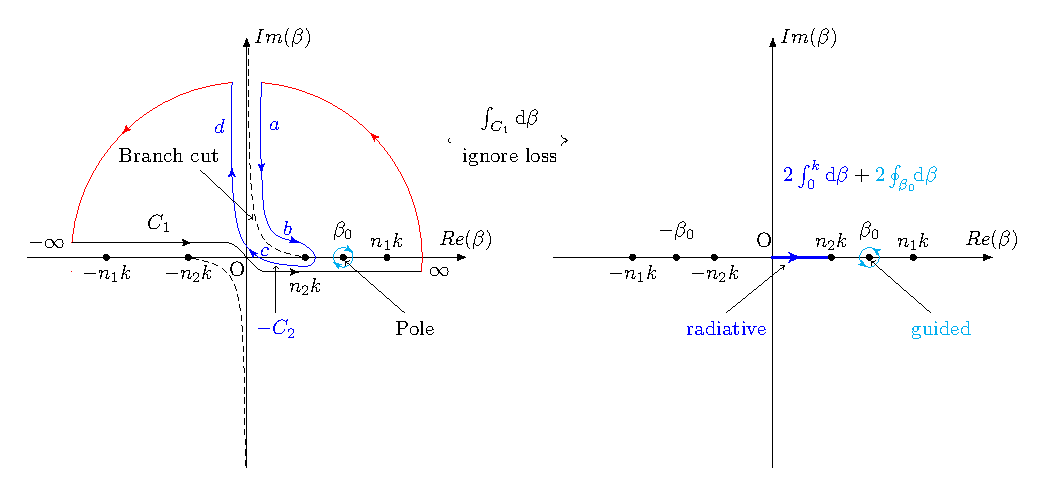
\includegraphics[scale=0.75]{../media/Figs/contourplot_upper}}
\end{minipage}
\par\medskip
\begin{minipage}{.91\linewidth}
\centering
\subfloat[]{\label{contourplot_lower}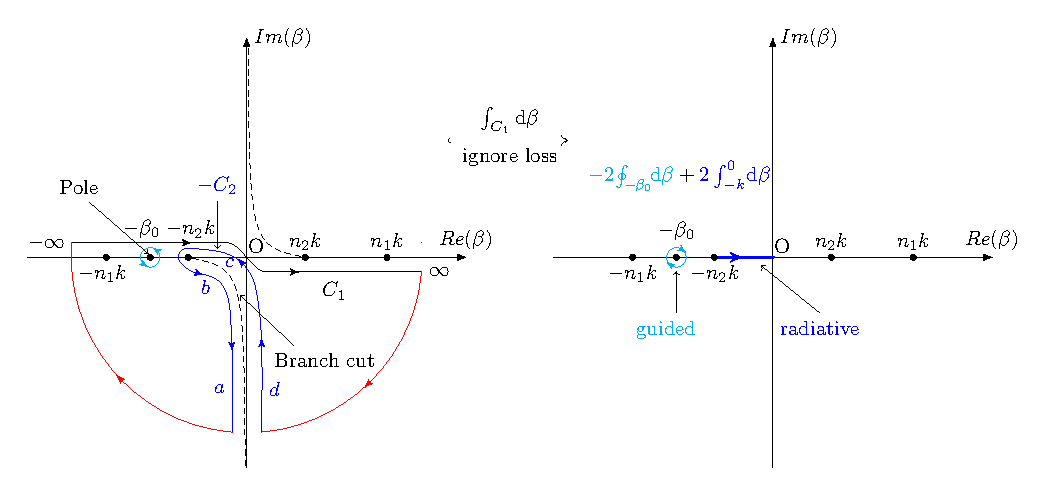
\includegraphics[scale=0.75]{../media/Figs/contourplot_lower}}
\end{minipage}
\caption[Contour integrations to decompose the guided and radiative modes of a dipole radiation problem in presence of a single mode waveguide.]{Integration paths. For the case that $ z>0 $, we can use the zero-valued contour integral path drawn in subfig.~\ref{contourplot_upper} to calculate the integration along path $ C_1 $. The simplified integration path by ignoring waveguide losses is given on the right-hand-side. It only contains the forward propagating mode contributions with radiation and guided mode components as divided through the real-axis integral and the loop-hole integral. For the $ z<0 $ case, the contour integral analysis is given in subfig.~\ref{contourplot_lower}, which only includes the backward propagating mode contributions.}
\label{fig:integralpath}
\end{figure}

Now, we only consider the $ m=\pm 1 $ modes, and hence Equs.~\ref{ET0Rexpand}, ~\ref{BT0Rexpand} and the corresponding $ \phi $ and $ r\!_\perp $ components can be explicitly expressed as contour integrals as below
\begin{subequations}\label{ET0RC1}
\begin{align}
\mathcal{E}^{(T)}_z &= \sum_{m=\pm 1} \int_{C_1} \mathrm{d}\beta e^{im(\phi-\phi') + i\beta (z-z')} c_{m\beta} J_m (hr\!_\perp),\\
% + B_{m\beta} Y_m(hr\!_\perp)\right],\\
\mathcal{E}^{(0)}_{z} &= \sum_{m=\pm 1} \int_{C_1} \mathrm{d}\beta e^{im(\phi-\phi') + i\beta (z-z')} \mathcal{E}^{(0)}_{z,m\beta}(r\!_\perp)\\
\mathcal{E}^{(R)}_z &= \sum_{m=\pm 1} \int_{C_1} \mathrm{d}\beta e^{im(\phi-\phi') + i\beta (z-z')} a_{m\beta} H_m^{(1)} (pr\!_\perp),
\end{align}
\end{subequations}
\begin{subequations}\label{BT0RC1}
\begin{align}
\mathcal{B}^{(T)}_z &= \sum_{m=\pm 1} \int_{C_1} \mathrm{d}\beta e^{im(\phi-\phi') + i\beta (z-z')} d_{m\beta} J_m (hr\!_\perp),\\
% + E_{m\beta} Y_m(hr\!_\perp)\right],\\
\mathcal{B}^{(0)}_{z} &= \sum_{m=\pm 1} \int_{C_1} \mathrm{d}\beta e^{im(\phi-\phi') + i\beta (z-z')} \mathcal{B}^{(0)}_{z,m\beta}(r\!_\perp)\\
\mathcal{B}^{(R)}_z &= \sum_{m=\pm 1} \int_{C_1} \mathrm{d}\beta e^{im(\phi-\phi') + i\beta (z-z')} b_{m\beta} H_m^{(1)} (pr\!_\perp).
\end{align}
\end{subequations}
To distinguish the bound and radiation modes contributions, one can use the integral path along $ C_1 $ (see Fig.(\ref{fig:integralpath})) and find the equivalent integral path detouring the branch cuts and isolated poles which will be discussed next. 

For the free-dipole radiation components, the $ C_1 $ integral path is almost the real integral path from $ -\infty $ to the $ +\infty $ except for the branch point at $ \pm k $. The sign of $ \beta $ indicates the propagation direction of the field. The free-dipole components only yield the radiation mode contributions to the total Green's dyadic. This is because the dipole radiation only occurs outside of the fiber, and always in the radiation potential zone using the equivalent scattering potential model. 

For the reflection and transmission components of the field, there are poles in the $ a_{m\beta} $, $ b_{m\beta} $, $ c_{m\beta} $ and $ d_{m\beta} $ coefficients. There are also branch cuts hidden in the Bessel and Hankel function components of their expressions. Depending on the sign of $ (z-z') $, the integral paths and their simplification are shown in Fig.(\ref{fig:integralpath}). The bound modes are associated with poles, and hence can be represented as residues if asymptotic approximation can be made. Therefore, the guided mode contribution part of the reflection and transmission components can be given by
\begin{subequations}\label{ET0RRes}
\begin{align}
\mathcal{E}^{(T)}_z &= \sum_{m=\pm 1} \oint_{\beta_{1,m}}  e^{im(\phi\!-\!\phi') + i\beta (z\!-\!z')} c_{m\beta} J_m (hr\!_\perp),\\
%\mathcal{E}^{(0)}_{z} &= 2\pi i \sum_{m=\pm 1} \sum_{\beta_{1,m=\pm 1}}\mathrm{Res}\left[  e^{im(\phi-\phi') + i\beta (z-z')} \mathcal{E}^{(0)}_{z,m\beta}(r\!_\perp)\right]_{\beta=\beta_{1,m}},\\
\mathcal{E}^{(R)}_z &= \sum_{m=\pm 1} \oint_{\beta_{1,m}} e^{im(\phi\!-\!\phi') + i\beta (z\!-\!z')} a_{m\beta} H_m^{(1)} (pr\!_\perp),
\end{align}
\end{subequations}
\begin{subequations}\label{BT0RRes}
\begin{align}
\mathcal{B}^{(T)}_z &= \sum_{m=\pm 1} \oint_{\beta_{1,m}} e^{im(\phi\!-\!\phi') + i\beta (z\!-\!z')} d_{m\beta} J_m (hr\!_\perp),\\
%\mathcal{B}^{(0)}_{z} &= 2\pi i \sum_{m=\pm 1} \sum_{\beta_{1,m=\pm 1}}\mathrm{Res}\left[  e^{im(\phi-\phi') + i\beta (z-z')} \mathcal{B}^{(0)}_{z,m\beta}(r\!_\perp)\right]_{\beta=\beta_{1,m}}, \\
\mathcal{B}^{(R)}_z &= \sum_{m=\pm 1} \oint_{\beta_{1,m}} e^{im(\phi\!-\!\phi') + i\beta (z\!-\!z')} b_{m\beta} H_m^{(1)} (pr\!_\perp).
\end{align}
\end{subequations}
%\begin{subequations}\label{ET0RRes}
%\begin{align}
%\mathcal{E}^{(T)}_z &= 2\pi i \sum_{m=\pm 1} \sum_{\beta_{1,m=\pm 1}}\mathrm{Res}\left[  e^{im(\phi\!-\!\phi') + i\beta (z\!-\!z')} c_{m\beta} J_m (hr\!_\perp)\right]_{\beta=\beta_{1,m}},\\
%% + B_{m\beta} Y_m(hr\!_\perp)\right],\\
%\mathcal{E}^{(0)}_{z} &= 2\pi i \sum_{m=\pm 1} \sum_{\beta_{1,m=\pm 1}}\mathrm{Res}\left[  e^{im(\phi-\phi') + i\beta (z-z')} \mathcal{E}^{(0)}_{z,m\beta}(r\!_\perp)\right]_{\beta=\beta_{1,m}},\\
%\mathcal{E}^{(R)}_z &= 2\pi i \sum_{m=\pm 1} \sum_{\beta_{1,m=\pm 1}}\mathrm{Res}\left[ e^{im(\phi\!-\!\phi') + i\beta (z\!-\!z')} a_{m\beta} H_m^{(1)} (pr\!_\perp)\right]_{\beta=\beta_{1,m}},
%\end{align}
%\end{subequations}
%\begin{subequations}\label{BT0RRes}
%\begin{align}
%\mathcal{B}^{(T)}_z &= 2\pi i \sum_{m=\pm 1} \sum_{\beta_{1,m=\pm 1}}\mathrm{Res}\left[ e^{im(\phi\!-\!\phi') + i\beta (z\!-\!z')} d_{m\beta} J_m (hr\!_\perp)\right]_{\beta=\beta_{1,m}},\\
%% + E_{m\beta} Y_m(hr\!_\perp)\right],\\
%\mathcal{B}^{(0)}_{z} &= 2\pi i \sum_{m=\pm 1} \sum_{\beta_{1,m=\pm 1}}\mathrm{Res}\left[  e^{im(\phi-\phi') + i\beta (z-z')} \mathcal{B}^{(0)}_{z,m\beta}(r\!_\perp)\right]_{\beta=\beta_{1,m}}, \\
%\mathcal{B}^{(R)}_z &= 2\pi i \sum_{m=\pm 1} \sum_{\beta_{1,m=\pm 1}}\mathrm{Res}\left[ e^{im(\phi\!-\!\phi') + i\beta (z\!-\!z')} b_{m\beta} H_m^{(1)} (pr\!_\perp)\right]_{\beta=\beta_{1,m}}.
%\end{align}
%\end{subequations}

The radiation mode contributions of the reflection and transmission components are associated with the branch cuts $ C_2 $~\cite{Klimov2004} in Fig.(\ref{fig:integralpath}).
\begin{subequations}\label{ET0RC2}
\begin{align}
\mathcal{E}^{(T)}_z &= \sum_{m=\pm 1} \int_{C_2} \mathrm{d}\beta e^{im(\phi-\phi') + i\beta (z-z')} c_{m\beta} J_m (hr\!_\perp)\\
&\approx \sum_{m=\pm 1} 2\int_{-n_2k}^{n_2k} \mathrm{d}\beta e^{im(\phi-\phi') + i\beta (z-z')} c_{m\beta} J_m (hr\!_\perp),\\
%\mathcal{E}^{(0)}_{z} &= \sum_{m=\pm 1} \oint_{C_2} \mathrm{d}\beta e^{im(\phi-\phi') + i\beta (z-z')} \mathcal{E}^{(0)}_{z,m\beta}(r\!_\perp),\\
\mathcal{E}^{(R)}_z &= \sum_{m=\pm 1} \oint_{C_2} \mathrm{d}\beta e^{im(\phi-\phi') + i\beta (z-z')} a_{m\beta} H_m^{(1)} (pr\!_\perp)\\
&\approx \sum_{m=\pm 1} 2\int_{-n_2k}^{n_2k} \mathrm{d}\beta e^{im(\phi-\phi') + i\beta (z-z')} a_{m\beta} H_m^{(1)} (pr\!_\perp),
\end{align}
\end{subequations}
\begin{subequations}\label{BT0RC2}
\begin{align}
\mathcal{B}^{(T)}_z &= \sum_{m=\pm 1} \oint_{C_2} \mathrm{d}\beta e^{im(\phi-\phi') + i\beta (z-z')} d_{m\beta} J_m (hr\!_\perp)\\
&\approx \sum_{m=\pm 1} 2\int_{-n_2k}^{n_2k} \mathrm{d}\beta e^{im(\phi-\phi') + i\beta (z-z')} d_{m\beta} J_m (hr\!_\perp),\\
%\mathcal{B}^{(0)}_{z} &= \sum_{m=\pm 1} \oint_{C_2} \mathrm{d}\beta e^{im(\phi-\phi') + i\beta (z-z')} \mathcal{B}^{(0)}_{z,m\beta}(r\!_\perp),\\
\mathcal{B}^{(R)}_z &= \sum_{m=\pm 1} \oint_{C_2} \mathrm{d}\beta e^{im(\phi-\phi') + i\beta (z-z')} b_{m\beta} H_m^{(1)} (pr\!_\perp)\\
&\approx \sum_{m=\pm 1} 2\int_{-n_2k}^{n_2k} \mathrm{d}\beta e^{im(\phi-\phi') + i\beta (z-z')} b_{m\beta} H_m^{(1)} (pr\!_\perp).
\end{align}
\end{subequations}
Above, the approximation works when the waveguide is lossless and hence the branch lines along the imaginary axis of the $ \beta $-plane can be ignored. The factor of $ 2 $ comes from the sign flip of the two branch lines parallel to the real axis in the $ \beta $ plane ($ 2=1-\mathrm{e}^{\pi i} $), and physically corresponds to the degeneracy of $ 2 $ degrees of freedom of the polarization of the radiation modes in the transverse plane. Although we use the integral limit from $ -n_2k $ to $ n_2k $, the integral limit, in practice, should be either $ 0 \rightarrow n_2k$ or $ -n_2k\rightarrow 0 $ depending on the propagation directions we are interested in. 

One can obtain the bound and radiation field components with the dipole oriented in $ z $, $ \phi $ and $ r\!_\perp $ directions by substituting the $ \bmc{E}^{(0)}_{m\beta}(r\!_\perp) $ expressions for corresponding cases into Equs.~\ref{ET0RRes},~\ref{BT0RRes},~\ref{ET0RC2} and~\ref{BT0RC2}. 

To calculate the bound modes, we need to calculate the residues at isolated poles with $ \beta_{1,m} $ and $ m=\pm 1 $. The poles can be found by using the condition that
\begin{align}
D=P^2+QR=0,
\end{align}
or
\begin{align}\label{pole4beta}
&\beta^2m^2k^4\left(J_m(ha) H_m^{(1)}(pa) \right)^2 (\varepsilon_f-1)^2\nonumber\\
-& h^2p^2a^2k^2 \left(hJ_m(ha) \dd{}{(pa)}H_m^{(1)}(pa)-pH_m^{(1)}(pa)\dd{}{(ha)}J_m(ha) \right)\nonumber\\ &\left(hJ_m(ha) \dd{}{(pa)}H_m^{(1)}(pa)-\varepsilon_f pH_m^{(1)}(pa)\dd{}{(ha)}J_m(ha) \right)=0.
\end{align}
Here are some useful relationships to solve the equation above:
\begin{align}
J_{-m}(z)=(-1)^nJ_n(z),\, &\quad H_{-m}^{(1)}(z)=e^{m\pi i}H_m^{(1)}(z),\\
\dd{}{z}J_m(z) &= \frac{1}{2} \left( J_{m-1}(z)-J_{m+1}(z) \right),\\ 
\dd{}{z}H^{(1)}_m(z) &= \frac{1}{2} \left( H^{(1)}_{m-1}(z)-H^{(1)}_{m+1}(z) \right).
\end{align}
We can rewrite Equ.~\ref{pole4beta} as
\begin{align}\label{pole4beta2}
&\beta^2m^2k^2\left(J_m\!(ha) H_m^{(\!1\!)}\!(pa) \right)^2 (\varepsilon_f-1)^2\nonumber\\
=& \frac{h^2p^2a^2}{4} \left[hJ_m\!(ha)\! \left( H^{(\!1\!)}_{m-1}\!(pa)\!-\! H^{(\!1\!)}_{m+1}\!(pa) \right)\!-\! pH_m^{(\!1\!)}\!(pa)\left( J_{m-1}\!(ha)\!-\! J_{m+1}\!(ha) \right) \right]\nonumber\\ 
&\left[hJ_m\!(ha) \left( H^{(\!1\!)}_{m-1}\!(pa)\!-\! H^{(\!1\!)}_{m+1}\!(pa) \right)\!-\! \varepsilon_f pH_m^{(\!1\!)}\!(pa)\left( J_{m-1}\!(ha)\!-\! J_{m+1}\!(ha) \right) \right].
\end{align}
Since both $ h $ and $ p $ are functions of $ \beta $, the equation above is complicated for solving $ \beta $. If $ ka<0.8 $, asymptotic approximation is good enough to solve Equ.~\ref{pole4beta2} and give an analytical solution for $ \beta $~\cite{Klimov2004}. However, in our nanofiber case, the $ ka<0.8 $ condition is not satisfied. We should be able to numerically solve Equ.~\ref{pole4beta2} for $ \beta $ as the characteristic constant for the guided mode with $ m=\pm 1 $. \textcolor{red}{Q: we should prove Equ.~\eqref{pole4beta2} is equivalent to the eigen equation of $ \beta $ for the bare fiber case. Useful relationship: $ K_n(x)=\frac{\pi}{2}i^{n+1}H_n^{(1)}(ix) $.}

Numerically, the eigenwavevector $ \beta_0 $ is indistinguishable with the intrinsic nanofiber eigen mode wavevector, in the regime we are interested in.

Next, we can solve the bound modes by differentiating the functions inside of $ Res $ signs and inserting the values of $ \beta_{1,m=\pm 1} $. %\textcolor{red}{(Q: are those poles all of order 1?)} 
The transverse components of the fields can be obtained from the longitudinal components using the relations of Equ.~\ref{EHzgauss}. 
%Sample numerical calculations has been performed, and results are documented in the NanofiberProjectPlots.pdf (Dropbox folder, \url{Nanofiber/Code/Matlab/Plots}). The primary plots show that there are phase shifts for the transmitted and reflected lights so that the mode profile is not symmetric to the $ x $-axis where the atom lies on; the reflected light field has a backaction on the atom tending to move it off the trapping point; the $ m=\pm 1 $ modes are not balanced... 
Our derivation results had be checked by reproducing the decay rates following Klimov's paper~\cite{Klimov2004}. 

To calculate the total decay rate of the atom with the enhancement due to the radiation, we need to find out the functions describing the branch cuts and the integration path for the radiation modes. The equation defining the branch cut is given by
\begin{align}\label{branchcutequ}
\mathrm{Im}\left[p \right] &=0\\
\mathrm{Im}\left[h\right] &=0.
\end{align}
By setting $ \beta=x+iy $, we can rewrite the first equation above as
\begin{align}
p&=\sqrt{k^2-\beta^2}\\
&=\left[(k^2-x^2+y^2)^2 + 4x^2y^2 \right]^{1/4}e^{\frac{i}{2}\arctan\frac{-2xy}{k^2-x^2+y^2}}.
\end{align}
Hence Equ.~\ref{branchcutequ} yields
\begin{align}
0&= \left[(k^2-x^2+y^2)^2 + 4x^2y^2 \right]^{1/4} \sin \left[\frac{1}{2}\arctan\frac{-2xy}{k^2-x^2+y^2} \right]\\
&= \frac{1}{\sqrt{2}} \left[(k^2\!-\! x^2\!+\! y^2)^2 \!+\! 4x^2y^2 \right]^{1/4} \sqrt{1\!-\!\cos \left(\arctan\frac{-2xy}{k^2\!-\! x^2\!+\! y^2} \right)}\\
&= \frac{1}{\sqrt{2}} \left[(k^2\!-\!x^2\!+\! y^2)^2 \!+\! 4x^2y^2 \right]^{1/4} \sqrt{1\!-\! \frac{k^2\!-\! x^2\!+\! y^2}{\left[(k^2\!-\! x^2\!+\! y^2)^2 \!+\! 4x^2y^2 \right]^{1/2}} }\\
&=\sqrt{\left[(k^2-x^2+y^2)^2 + 4x^2y^2 \right]^{1/2}-(k^2-x^2+y^2)},
\end{align}
which gives
\begin{align}
\left[(k^2-x^2+y^2)^2 + 4x^2y^2 \right]^{1/2}&=(k^2-x^2+y^2),\\
\Leftrightarrow \qquad \qquad \qquad \qquad \qquad x^2y^2&=0.\label{branchcut2}
\end{align}
Obviously, the $ x $-axis between $ [-k,k] $ and the entire $ y $-axis are the branch cuts. To separate the branches into upper and lower parts, we can define an arbitrary small positive number $ \delta\epsilon\rightarrow 0 $ so that Equ.~\ref{branchcut2} gives
\begin{align}
xy&=\delta\epsilon.
\end{align}
Similarly, the condition for $ \mathrm{Im}[h]=0 $ gives the same result. To make the field components homomorphic at any point in the complex $ \beta $ plane, we choose the branch cuts that satisfy 
\begin{align}
xy&>\delta\epsilon>0.
\end{align}
Calling the physics meaning of radiation mode, we also have 
\begin{align}
-n_2k<x<n_2k.
\end{align}
In this way, the branch cuts as a hyperbola-type lines are symmetrically separated into top-right and lower-left parts, and are very close to the $ x- $ and $ y- $axes. For the top-right branch, one can choose the integration path as shown in Fig.~\ref{fig:integralpath} to apply the contour integral detouring the branch cut. 

%\scalefig{Figs/contourpath2}{0.8}{Integration path of the contour integral for radiation modes.}

In the case that the nanofiber can be treated as a lossless medium, the contour integral can be treated as an integral over real axis from $ -kn_2 $ to $ kn_2 $. 

%\textcolor{red}{Current issue: there is a divergence problem of calculating the guided mode contribution in the limit of $ r \rightarrow \infty $. To reduce the error, we need to carefully choose a proper integral path when we integrate around the pole to obtain the guided mode contributions (contour radius matters). However, in the regime we are interested in, the error is negligible. If we can prove that the guided mode contribution from the free-space radiation is always zero, then the numerical result of the free-space bounded mode contribution can be used to estimate numerical errors in our bounded mode contribution calculations.  }



%One technical difficulty is the contour integral around the branch cut. We have used a numerical calculus package called Chebfun~\footnote{See \url{http://www2.maths.ox.ac.uk/chebfun/} for details.} to integrate over the contour path detouring the branch cut. Chebfun can find the polynomial approximations to an arbitrary function in a piecewise way by adaptively sampling a few points of the original function. The main issue of doing the contour integral is divergence using limited sampling points. Fig. shows two examples of the contour integral along the branch cut. 





\textcolor{red}{Pointing vectors and energy distribution...}

\textcolor{red}{Define transmitting and reflecting rates...}





\section{Green function formalism for the atom-waveguide system}
So far, we have studied two basic aspects for the waveguide boundary value problem: one is the eigenmode problem, in which we studied the permitted guided waveguide modes propagating along the waveguide in absence of atoms; the other one is the single-dipole radiation problem, in which we studied the propagating modes when there is a dipole radiating electromagnetic wave around a waveguide. Now, we can combine the conclusions of the two cases studied, and to study the full radiation reaction problem of the dipole-waveguide system, in which we assume there is a guided mode incident to the waveguide, and then excites one atom outside of the waveguide which radiates light into the waveguide and interferes with the waveguide modes. 


\begin{figure}
\centering\makebox[\textwidth]{
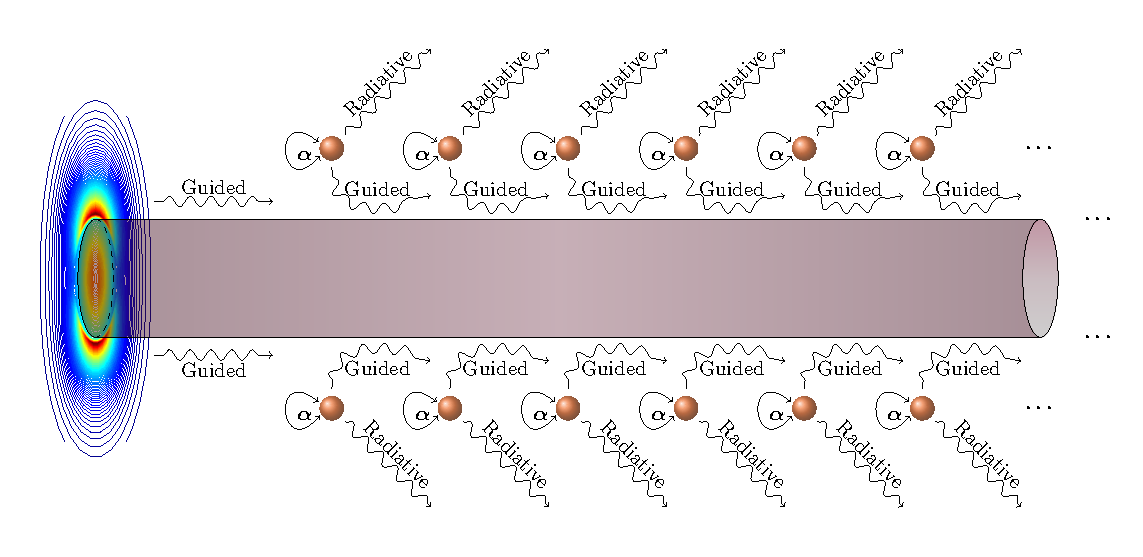
\includegraphics[width=0.85\textwidth]{../media/Figs/NanofiberTrappedAtoms}}
\caption{Diagram of nanofiber trapped atoms. }
\end{figure}

For our nanofiber case, only $ m=\pm 1 $ $ \text{HE}_{11} $ modes are permitted and guided. We assume the input mode is $ m=+1 $ $ \text{HE}_{11} $ guided mode, which can be written as 
\begin{align}
\mathbf{E}_0(\br,\omega_0)&=E_0 \mathbf{u}^+(r\!_\perp ) e^{i(\beta_0 z+\phi)}, 
\end{align}
where $ \mathbf{u}^{+}(r\!_\perp ) $ denotes the normalized bare nanofiber HE11 transverse mode with forward propagation counterclockwise rotation and circularly polarized light input. Similarly, $ \mathbf{u}^{-}(r\!_\perp ) $ is the forward propagating but clockwise rotating quasi-circular HE11 mode. In general, we denote  $ \mathbf{u}^{\mu}(r\!_\perp ) $ as the normalized $\mu=(\omega,f,p)$ mode radial components, with $ f=\pm $ denoting forward or backward propagating direction, $ p=\pm $ denoting counter-clockwise or clockwise rotation of polarization. For short, we denote $\mathbf{u}^+(r\!_\perp )$ as the forward-propagating and counter-clockwise-rotating $m=1$ guided mode. We also denote $ \beta_0 $ as the eigen wavenumber determined by the fiber eigenvalue  equation. Similarly, we denote $ \mathbf{u}^{\nu}(r\!_\perp ) $ as the radiation mode with mode index $ \nu=(\omega,\beta,m,p) $, where $ m=0,\,\pm 1,\,\pm 2,\cdots $ is the mode index, and $p=\pm$ denotes the polarization pattern. The guided and radiation modes satisfy the orthogonality conditions that 
\begin{align}
\int_0^{2\pi}\mathrm{d}\phi \int_0^\infty n_{r}^2|\mathbf{u}^{(\mu)}(r\!_\perp )|^2r\!_\perp \mathrm{d}r\!_\perp &=1,\\
\int_0^{2\pi}\mathrm{d}\phi \int_0^\infty n_{r}^2\left[\mathbf{u}^{(\nu)}(r\!_\perp )\cdot\mathbf{u}^{(\nu')*}(r\!_\perp )\right]_{\beta=\beta',m=m'}r\!_\perp \mathrm{d}r\!_\perp &=\delta(\omega-\omega')\delta_{pp'}.
\end{align}
The completeness relationships of the modes can be given by
\begin{align}
\sum_{f,p}\int \mathrm{d}\mathbf{k} \,n_r^2\mathbf{u}^{(\mu)}(r\!_\perp )\mathbf{u}^{(\mu)*}(r'\!_\perp ) &= \unittensor\delta^T(r\!_\perp-r'\!_\perp),\\
\sum_{m,p}\int \mathrm{d}\mathbf{k} \, n_r^2\mathbf{u}^{(\nu)}(r\!_\perp )\mathbf{u}^{(\nu)*}(r'\!_\perp ) &=\unittensor\delta^T(r\!_\perp-r'\!_\perp).
\end{align}

As shown in the earlier sections, in general, the output field in presence of a single atom can be written as
\begin{align}
\mathbf{E}(\br) 
&=\mathbf{E}_0(\br)+\alpha \GFT(\br,\br')\cdot \mathbf{E}_0(\br')
\end{align}
where we only treat the polarizability as a scalar. The only barrier for solving the output E-field is to solve the dyadic Green function.

In general, there are two strategies to solve the dyadic Green function: one is to solve the dipole emission problem numerically; the other one involves transverse mode decomposition and only needs bare fiber modes. We call the first approach as the \textit{normal} approach, and call the other one as the \textit{approximate} approach. We will describe the two approaches in the successive paragraphs. 

The \textit{normal} approach:

We recall that the equation governs the dyadic Green function can be written as below:
\begin{align}
\left[ -\nabla\times\nabla\times + n^2\frac{\omega^2_0}{c^2} \right] \GFT(\br,\br') &= -4\pi k_0^2\delta^{(3)}(\br-\br')\unittensor,
\end{align}
each column of which can be expressed as
\begin{align}
\left[ -\nabla\times\nabla\times + n^2\frac{\omega^2_0}{c^2} \right] \mathbf{G}_i(\br,\br') &= -4\pi k_0^2\mathbf{e}_i\delta(\br-\br'), \label{eq:Gi}
\end{align}
where the subscription $ i=r\!_\perp,\phi,z $ denotes the coordinate components. The $ \mathbf{G}_i(\br,\br') $ in the equation above is the $ i^{th} $ column of the dyadic Green function of $ \GFT(\br,\br') $. Here, we used $\omega_0$ to indicate the angular frequency of the radiation from the source.  

Comparing Equ.~\eqref{eq:Gi} with Equ.~\eqref{eq:Maxwellwithsource2}, we find that Equ.~\eqref{eq:Gi} is exactly the chromatic wave equation of $ \mathbf{E}(\br) $ when there is a dipole source orientated along $ \mathbf{e}_i $ direction and placed at $ \br' $ with an amplitude of $ -4\pi k^2 $. That is to say that once we solve the electric field components with a unit dipole source orientated along all $ \mathbf{e}_i $ directions, the columns of the dyadic function is just the corresponding field components divided by the factor of $ -4\pi k^2 $. Concretely, in the cylindrical coordinate system, the dyadic Green function elements correspond to the following electric field components emitted by a unit dipole source orientated in the three orthogonal basis:
\begin{equation}
\GFT(\mathbf{r},\mathbf{r}')=\!\!\!\!\!\!\!\!\!\!\!\!\!\!\!\!\!\!\!\!\!\!\!\! \!\!\!\!\!\!\!\! \!\!\!\!\!\!\!\! \!\!\!\!\!\!\!\!
  \begin{tikzpicture}[baseline=-\the\dimexpr\fontdimen22\textfont2\relax ]
   \matrix (m)[matrix of math nodes,left delimiter=(,right delimiter=),ampersand replacement=\&] % Note: the ampersandreplacement line redefines to use \& instead of the usual & sign to separate columns in the matrix. This can avoid potential conflict with external environment where ampersands are also defined for specific purposes. See https://tex.stackexchange.com/questions/15093/single-ampersand-used-with-wrong-catcode-error-using-tikz-matrix-in-beamer
  {
  G_{r\!_\perp r\!_\perp} \& G_{r\!_\perp\phi} \& G_{r\!_\perp z}\\
  G_{\phi r\!_\perp} \& G_{\phi\phi} \& G_{\phi z} \\
  G_{zr\!_\perp} \& G_{z\phi} \& G_{zz} \\
  };
  % Hightlight columns.
  \begin{pgfonlayer}{myback}
    \fhighlight[red!30]{m-1-1}{m-3-1}
    \fhighlight[blue!30]{m-1-2}{m-3-2}
    \fhighlight[green!30]{m-1-3}{m-3-3}
  \end{pgfonlayer}
  % Make links to other equivalent expressions.
  \begin{pgfonlayer}{myback}
    \draw (m-3-1.south)+(-0.5,-0.76) node [left] {column vector $\mathbf{G}_i$:};
    \draw[implies-implies,double equal sign distance] (m-3-1.south)+(0,-0.08) -- +(0,-0.5) node[below]{$ \mathbf{G}_{r\!_\perp} $};
    \draw[implies-implies,double equal sign distance] (m-3-2.south)+(0,-0.08) -- +(0,-0.5) node[below]{$ \mathbf{G}_{\phi} $};
    \draw[implies-implies,double equal sign distance] (m-3-3.south)+(0,-0.1) -- +(0,-0.55) node[below]{$ \mathbf{G}_z $};
    \draw (m-3-1.south)+(-0.5,-1.7) node [left,align=center] {equivalent $ \mathbf{E} $ radiated\\ from a unit dipole:};
    \draw[<-] (m-3-1.south)+(0,-1.08) -- +(0,-1.5) node[below]{$ \mathbf{d}_{r\!_\perp} $};
    \draw[<-] (m-3-2.south)+(0,-1.08) -- +(0,-1.5) node[below]{$ \mathbf{d}_{\phi} $};
    \draw[<-] (m-3-3.south)+(0,-1.1) -- +(0,-1.55) node[below]{$ \mathbf{d}_z $};
    \draw[<-] (m-3-3.south)+(0.5,-1.32) -- +(1.1,-1.32) node[right]{$\cdot (-4\pi k^2)$};
  \end{pgfonlayer}
  \end{tikzpicture}
\end{equation}
%\textcolor{red}{Need to make it look nicely, and continue on...}
The equivalent $ \mathbf{E} $ field has been solved in section~\ref{sec:boundrad} for the radiation problem with one atom.


The \textit{eigenmode decomposition} approach:

In the case that the source is extremely small, the total dyadic Green function should be effectively equal to the transverse dyadic Green function. To illustrate this idea, we can expand the current source of the dipole into transverse and longitudinal parts by
\begin{align}
\mathbf{J}(\br) &= \mathbf{J}_T(\br) + \mathbf{J}_L(\br),
\end{align}
where the transverse and longitudinal current components, $ \mathbf{J}_T(\br) $ and $\mathbf{J}_L(\br)$, satisfy
\begin{align}
\nabla\cdot\mathbf{J}_T (\br) &=0\\
\nabla\times \mathbf{J}_L (\br) &=0.
\end{align}
In SI units, the continuity condition reads
\begin{align}
\nabla\cdot\mathbf{J}=-\pp{}{t}\rho.
\end{align}
Under Coulomb gauge, the transverse and longitudinal currents can then be written as 
\begin{align}
\mathbf{J}_T &= -\frac{1}{\mu_0}(\nabla^2 -\frac{1}{c^2}\spp{}{t})\mathbf{A}\label{eq:Jt_cg}\\
\mathbf{J}_L &= \varepsilon_0 \pp{}{t}\nabla\phi .\label{eq:Jl_cg}
\end{align}
Notice that, the longitudinal current equation (Equ.~\eqref{eq:Jl_cg}) will become purely local for an ideal dipole source, and can be ignored. The longitudinal components may only become important for the case with a charged source. Below, we only consider the transverse eigenmode decompositions for our analysis of neutral atoms that can be treated as neutral point dipole sources.

The dyadic Green's function for a waveguide satisfies (Equ.~\eqref{eq:dyadicGF})
\begin{align}
\left[ -\nabla\times\nabla\times + n^2k_0^2 \right] \GFT(\br,\br') &= -4\pi k_0^2\delta^{(3)}(\br-\br')\unittensor,
\end{align}
where $n=n(\br\!_\perp)=\sqrt{\varepsilon(\br\!_\perp)}$ and $k_0=\omega_0/c$. Correspondingly, the bare-fiber modes (eigenmodes), $ \mathbf{u}^{(\mu)}(\br) $, satisfy the Maxwell-Helmholtz equation (Equ.~\eqref{MaxwellHelmholtz0}), that is
\begin{align}
[-\nabla\times\nabla\times + n^2(\br)k^2]  \mathbf{u}^{(\mu)}(\br) &=0,
\end{align}
where $ k^2=\frac{\omega_{\mathbf{k}}^2}{c^2} $ and $ \mathbf{k} $ is an arbitrary wave vector.

To use the eigenfunction expansion method to calculate the dyadic Green function, we can define a vector function
\begin{align}
{\mathbf{u}}_\epsilon^{(\mu)}(\br) &= n(\br) \mathbf{u}^{(\mu)}(\br),
\end{align}
which satisfies
\begin{align}
\left[-\frac{1}{n(\br)}\nabla\times\nabla\times \frac{1}{n(\br)} + k^2\right]  {\mathbf{u}}_\epsilon^{(\mu)}(\br) &=0.
\end{align}
Introduced by Glauber and Lewenstein~\cite{Glauber1991}, the operator on the left-hand-side of the equation above, $\mathcal{H}_k = -\frac{1}{n(\br)}\nabla\times\nabla\times \frac{1}{n(\br)} + k^2$, is always Hermitian. Similarly, we can define a Hermitian operator $\mathcal{H}_{k_0} = -\frac{1}{n(\br)}\nabla\times\nabla\times \frac{1}{n(\br)} + k_0^2$, and obtain the eigenequation with $\mathcal{H}_{k_0}$ given by
\begin{align}
\mathcal{H}_{k_0} \mathbf{u}_\epsilon^{(\mu)} &= \lambda_\mu \mathbf{u}_\epsilon^{(\mu)},
\end{align}
which has a set of eigensolutions $ (\mathbf{u}_\epsilon^{(\mu)},\lambda_\mu=k_0^2-k^2) $. There exists a set of adjoint eigensolutions $ (\tilde{\mathbf{u}}_\epsilon^{(\mu)},\lambda_\mu^*) $ to $\mathcal{H}_{k_0}^\dagger \tilde{\mathbf{u}}_\epsilon^{(\mu)} = \lambda_\mu^* \tilde{\mathbf{u}}_\epsilon^{(\mu)}$, such that the biorthogonality relation
\begin{align}
\int \mathbf{u}_\epsilon^{(\mu)} (\br)\cdot \left[\tilde{\mathbf{u}}_\epsilon^{(\mu')}(\br) \right]^* \mathrm{d}\br &= \int n^2(\br) \mathbf{u}^{(\mu)} (\br)\cdot {\mathbf{u}^{(\mu')}}^*(\br) \mathrm{d}\br=\delta_{\mu\mu'},\label{eq:orthutrans}
\end{align}
and the completeness relation
\begin{align}
\sum_\mu \mathbf{u}_\epsilon^{(\mu)} (\br) \left[\tilde{\mathbf{u}}_\epsilon^{(\mu)}(\br') \right]^* &= \sum_\mu n(\br)n(\br') \mathbf{u}^{(\mu)} (\br) {\mathbf{u}^{(\mu)}}^*(\br) =\eye \delta^{(3)}(\br-\br'). 
\end{align}
In our nanofiber case, we can define such a set of mode functions, and in fact we choose them to have the following properties for their adjoint functions:
\begin{align}
\tilde{\mathbf{u}}_\epsilon^{(\mu)}(\br) &= n^*(\br) \tilde{\mathbf{u}}^{(\mu)}(\br)\\
\tilde{\mathbf{u}}^{(\mu)}(\br) &= {\mathbf{u}^{(\tilde{\mu})}}^*(\br)\\
{\mathbf{u}^{(\tilde{\mu})}}(\br) &= {\mathbf{u}^{(\mu)}}^*(\br)
\end{align}
with $ \tilde{\mu}=(\omega_0,-m,-f) $. For a single-mode nanofiber, we let $ n(\br)=n(\br\!_\perp) $ be real and define $ \mathbf{u}^{(\mu)}(\br)=\mathbf{u}_{mf}(r\!_\perp )e^{if\beta z+im\phi} $ for the guided $\mathrm{HE}_{11}$ modes with a propagation constant $ \beta  $. The completeness relation for the normalized modes will yield a transverse $ \delta $-function, $ \delta^T(\br-\br') $, having the property that
\begin{align}
\mathbf{f}^T(\br')&=\int \mathrm{d}\br\,\, \delta^T(\br-\br')\mathbf{f}(\br).
\end{align} 
Similar to the integration in the general biorthogonality relationship, if we only integrate over the transverse plane of a mode, we will obtain
\begin{align}
\int_0^{2\pi}\!\!\!\!\! \mathrm{d}\phi\!\! \int_0^\infty\!\!\!\! r\!_\perp \mathrm{d}r\!_\perp  n^2(r\!_\perp) \mathbf{u}_{mf}(r\!_\perp )\!\cdot\!\mathbf{u}_{m'f'}^*(r\!_\perp )& e^{i(f\!-\!f')\beta z+i(m\! -\! m')\phi}  =\delta_{mm'}e^{i(f\!-\!f')\beta z} \label{eq:orthutrans2D}.
\end{align}


From those eigensolutions, we can define a dyad, $ \mathbf{G}_\epsilon(\br,\br') $, satisfying
\begin{align}
\mathbf{G}_\epsilon(\br,\br') &= n(\br) \mathbf{G}(\br,\br') n(\br'),\\
\mathcal{H}_{k_0} \mathbf{G}_\epsilon(\br,\br') &= \mathbbm{1}\delta^{(3)}(\br-\br').\label{eq:HGtilde}
\end{align}

One can expand the dyadic function $ \mathbf{G}_\epsilon(\br,\br') $ in terms of the transverse eigenmodes by
\begin{align}
\mathbf{G}_\epsilon(\br,\br')\approx\mathbf{G}_\epsilon^T(\br,\br')= \sum_{\mu} \mathbf{u}_\epsilon^{(\mu)}(\br) \mathbf{A}_\epsilon^{(\mu)}(\br'), \label{eq:transGappr}
\end{align}
where the coefficient vector $\mathbf{A}_\epsilon^{(\mu)}(\br')  $ does not depend on $ \br $.
Substituting Equ.~\eqref{eq:transGappr} into Equ.~\eqref{eq:HGtilde}, we obtain
\begin{align}
\sum_{\mathbf{k}} \left[ \mathcal{H}_{k_0}  \mathbf{u}_\epsilon^{(\mu)}(\br)\right] \mathbf{A}_\epsilon^{(\mu)}(\br') &= -4\pi k_0^2\mathbbm{1}\delta^{(3)}(\br-\br')\\
\Leftrightarrow \sum_\mu (k_0^2-k^2) \mathbf{u}_\epsilon^{(\mu)}(\br) \mathbf{A}_\epsilon^{(\mu)}(\br') &= -4\pi k_0^2\mathbbm{1}\delta^{(3)}(\br-\br') = -4\pi k_0^2\sum_{\mu} \mathbf{u}_\epsilon^{(\mu)}(\mathbf{r} )\left[\tilde{\mathbf{u}}_\epsilon^{(\mu)}(\mathbf{r}^\prime )\right]^*.
\end{align}
Therefore, we can solve the coefficient vector for an arbitrary eigenmode to give
\begin{align}
\mathbf{A}_\epsilon^{(\mu)}(\br') &= -4\pi\frac{\omega_0^2 \left[ \tilde{\mathbf{u}}_\epsilon^{(\mu)}(\br')\right]^*}{\omega_0^2-\omega_{\mathbf{k}}^2}.
\end{align}
Hence, 
\begin{align}
\mathbf{G}_\epsilon(\br,\br')= -4\pi\sum_{\mu} \frac{\omega_0^2\mathbf{u}_\epsilon^{(\mu)}(\br)\left[\tilde{\mathbf{u}}_\epsilon^{(\mu)}(\br')\right]^*}{\omega_0^2-\omega_{\mathbf{k}}^2} = -4\pi n(\br) \left[\sum_{\mu} \frac{\omega_0^2 {\mathbf{u}}^{(\mu)}(\br) {\mathbf{u}^{(\mu)}}^*(\br')}{\omega_0^2-\omega_{\mathbf{k}}^2} \right]n(\br').
\end{align}
By the definition of $\mathbf{G}_\epsilon(\br,\br')  $, the dyadic Green function can be written by 
\begin{align}
\mathbf{G}(\br,\br')\approx -4\pi\sum_{\mu} \frac{\omega_0^2\mathbf{u}^{(\mu)}(\br) {\mathbf{u}^{(\mu)}}^*(\br')}{\omega_0^2-\omega_{\mathbf{k}}^2}.
\end{align}
For the guided $\mathrm{HE}_{11}$ modes, we have 
\begin{align}
\mathbf{G}^g(\br,\br') &= -4\pi\sum_{\beta,m,f=\pm 1} \frac{\omega_0^2\mathbf{u}_{\mu}(r\!_\perp)\mathbf{u}^*_{\mu}(r_{\!\perp}^\prime)}{\omega_0^2-\omega_\beta^2}e^{if\beta(z-z')+im(\phi-\phi')},\label{eq:Gganaly}
\end{align}
where $ \omega_\beta $ is the angular frequency of the guided HE11 modes with the amplitude $ z $-component of the wave vector being $ \beta $. \textcolor{red}{The mode index should be $ \mu=(\beta_0,m=\pm 1,f=\pm 1) $. This notation should be unified starting here.} Now, we can use the dispersion expansion of $ \omega_\beta $ around $ \omega_0 $ with a group velocity $ v_g $ that 
\begin{align}
\omega_\beta &=\omega_0 + \dd{\omega_\beta}{\beta}(\beta-f\beta_0) +\cdots = \omega_0 + fv_g(\beta-f\beta_0) +\cdots\\
\Rightarrow \omega_\beta - \omega_0 &= fv_g(\beta-f\beta_0) +\cdots
\end{align}
Meanwhile, the sum over the mode index can be written as an integral over $ \beta $:
\begin{align}
\sum_{\beta} \Leftrightarrow & \frac{L}{2\pi} \int_{-\infty}^{\infty} \mathrm{d}\beta, \quad \text{if $\beta$ includes the propagation direction},\\
\quad \mathrm{or}\quad &\frac{L}{2\pi}\sum_{f=\pm 1} \int_0^{\infty} \mathrm{d}\beta,\quad\text{if the propagation direction is separated out}.
\end{align}
This  transformation comes from the consideration that, in the continuous limit, the propagating guided wave is periodic within the quantization length period $ L $ and the periodicity condition is that $ \beta_n L=2\pi n $, where $ n=1,\,2,\,\ldots $. Hence, the dyadic Green function for the guided modes (Equ.~\eqref{eq:Gganaly}) can be written as
\begin{align}
\!\!\!\!\!\!\!\!\! \mathbf{G}^g(\br,\br') &= -2L\sum_{m,f=\pm 1}\int_0^\infty \mathrm{d}\beta \frac{\omega_0^2\mathbf{u}_{m}(r\!_\perp)\mathbf{u}^*_{m}(r_{\!\perp}^\prime)}{\omega_0^2-\omega_\beta^2}e^{if\beta(z-z')+im(\phi-\phi')}\\
&= 2\omega_0^2 L\!\!\sum_{m,f=\pm 1}\int_0^\infty\!\! \mathrm{d}\omega_\beta \frac{\mathrm{d}\beta}{\mathrm{d}\omega_\beta} \frac{\mathbf{u}_{m}(r\!_\perp)\mathbf{u}^*_{m}(r_{\!\perp}^\prime)}{(\omega_0\! +\!\omega_\beta) (\omega_0\!-\!\omega_\beta)} e^{i\!f\!\beta(z\!-\!z')+im(\phi\!-\!\phi')}\label{eq:eigGFintegral}\\
&\approx 2\omega_0^2L \!\!\! \sum_{m,f=\pm 1}\!\!\!\!\! \pi i\,\!  \frac{f}{fv_g} \mathrm{Res}\!\! \left[\! \frac{\mathbf{u}_{m}\!(r\!_\perp\! ) \mathbf{u}^*_{m}\! (r_{\!\perp}^\prime\! ) e^{i\! f\! \beta(z \!-\! z')+im(\phi\!-\! \phi')} }{(\omega_0+\omega_\beta)(\omega_0-\omega_\beta)} \!\right]\!\!\!\!_{\begin{array}{l} \omega_\beta\! =\!\omega_0 \\ \beta\! =\!\beta_0\end{array} }\\
&= \pi\frac{iL}{v_g} \sum_{m,f=\pm 1} \mathbf{u}_{m}(r\!_\perp)\mathbf{u}^*_{m}(r_{\!\perp}^\prime)e^{if\beta_0(z-z')+im(\phi-\phi')},
\end{align}
where $ \beta_0 $ is the propagation constant with a given $ \omega_0 $ for the input/emission field. The integral path and the equivalence to the residue at $ \beta_0 $ is illustrated in part (c) of Fig.(\ref{fig:integralpaths}). We have used the fact that $ \int_{0-if\epsilon}^{\infty-if\epsilon} \mathrm{\omega_\beta}g(\omega_\beta) = P\left[ g(\omega_\beta)\right] +f\pi i \mathrm{Res}\left[g(\omega_\beta) \right] $, and ignored the principal value integral part, $ P\left[ g(\omega_\beta)\right] $. The principal value part yields the level shift of the atom due to the fiber modes, which should be negligible in the dispersive regime we are considering about. \todo[inline]{Note: the figure of integral path needs to be changed to have integrals always from $0$ to $\infty$ for $\omega_\beta$ and choose the shift of the integral path based on the sign of $f(z-z')$.} 

By using the relation that 
\begin{align}
k_0 &=\frac{\omega_0}{c}\\
n_g&=\sqrt{\varepsilon_g}= \frac{c}{v_g}
\end{align}
the dyadic Green function for the guided modes can also be written as
\begin{align}
\mathbf{G}^g(\br,\br') &\approx i\pi n_gL\sum_{m,f=\pm 1} \mathbf{u}_{m}(r\!_\perp)\mathbf{u}^*_{m}(r_{\!\perp}^\prime)e^{if\beta_0(z-z')+im(\phi-\phi')}.
\end{align}
We make $ L=1 $ for now, which should be canceled through multiplying with the quantization factor. 
 


The numerical comparison of the two approaches has been done and confirmed that these two approaches match up really well as long as we treat the integration paths under the same physics scenario.  

\begin{figure}
\centering\makebox[\textwidth]{
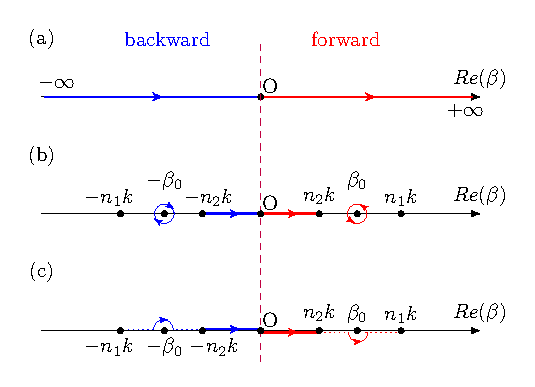
\includegraphics[width=0.85\textwidth]{../media/Figs/integratepath_GF}}
\caption[Integral paths for the dyadic Green function calculations when loss is negligible.]{Integral paths for the dyadic Green function calculations. Part (a) is the integral path for the dipole's free-space field contribution calculation (see, for example, Equ.~\eqref{ET0RC1}). Part (b) is the integral path for the reflected and transmitted field contributions calculation (see, for example, Equ.~\eqref{ET0RC1}). Part (c) is the integral path for the dyadic Green function calculation using the eigenmode decomposition method (see Equ.~\eqref{eq:eigGFintegral}). The integral paths on the left-hand-side (in blue) indicate the backward propagating contributions, while the right-hand-side (in red) parts corresponding to the forward propagating contributions. For the eigenmode decomposition method in part (c), if one choose to use $ f=\pm 1 $ to indicate the propagation direction, then only the $ \beta>0 $ portion of integral path will be applied. }
\label{fig:integralpaths}
\end{figure}

As shown in an earlier section, the guided and radiation modes contribution to the dyadic Green function can be identified through the specific choice of integral paths. In Fig.~\ref{fig:integralpaths}, part (a) shows the integral path to calculate the dipole free-space contribution which does not yield guided mode contribution to the total dyadic Green function. Part (b) of the figure shows the loop and real-valued integral paths of the guided and radiation mode divisions to the reflected and transmitted field components. The $ \mathrm{Re}(\beta)<0 $ and $ \mathrm{Re}(\beta)>0 $ parts correspond to the backward and forward propagating contributions, respectively. Part (c) of the figure indicates the integral path using the eigenmode decomposition method in the case that the sign of $ \mathrm{Re}(\beta) $ indicates the propagation directions. Depending on the propagation directions, we should choose the right integral paths for the corresponding methods adopted, and different methods should yield the same result. 

For the decay rate calculation, both forward and backward propagation contributions should be averaged, or just include one direction.  


\subsection{Calculation of group velocity and group index of refraction ($ v_g $ and $ n_g $)}
For a guided mode in a waveguide, the phase index of refraction is defined as
\begin{align}
n_p &= \frac{\beta}{k}.
\end{align}
Correspondingly, the group velocity and group index of refraction for a guided mode in a waveguide can be given by
\begin{align}
v_g &= \dd{\omega}{\beta},\\
n_g &= \frac{c}{v_g}=\dd{\beta}{k}.
\end{align}
Therefore, the group velocity and group index of refraction of the $ HE_{11} $ mode can calculated from the eigen function of $ \beta $ (see Appendix A of Ref.~\cite{LeKien2005a}). 

In general, the eigen function of $ \beta $ can be expressed as
\begin{align}
f(h,q,k,\beta) &=0
\end{align}
with $ h $ and $ q $ are both functions of $ k $ and $ \beta $. 
We differentiate the equation above with respect to $ \beta $ on both sides, and obtain
\begin{align}
\dd{f}{\beta} &= \pp{f}{h} \left(\pp{h}{k}\dd{k}{\beta}+\pp{h}{\beta} \right) + \pp{f}{q}\left(\pp{q}{k}\dd{k}{\beta}+\pp{q}{\beta} \right) +\pp{f}{k}\dd{k}{\beta}+\pp{f}{\beta}=0\\
\Rightarrow & \left( \pp{f}{h}\pp{h}{k}+\pp{f}{q}\pp{q}{k}+\pp{f}{k} \right)\dd{k}{\beta} = -\left(\pp{f}{h}\pp{h}{\beta}+\pp{f}{q}\pp{q}{\beta}+\pp{f}{\beta} \right)
\end{align}
\begin{align}
\Rightarrow &\quad\quad n_g = \dd{\beta}{k} = -\frac{\pp{f}{h}\pp{h}{k}+\pp{f}{q}\pp{q}{k}+\pp{f}{k}}
{\pp{f}{h}\pp{h}{\beta}+\pp{f}{q}\pp{q}{\beta}+\pp{f}{\beta}}.
\end{align}

Physically, the group index of refraction indicates the waveguide dispersion for a given propagating mode. Here, we can ignore the material dispersion due to the small response delay of the silica molecules of the waveguide substrate. Since the waveguide dispersion is merely a property of the waveguide, the presence of the radiating atom does not affect the group index of refraction at all (have checked numerically through solving the eigen function of $ \beta $ in presence of an atom). 

From the perspective of energy flowing, the group velocity can also be given by
\begin{align}
v_g&=\frac{P}{W}.
\end{align}
The physics interpretation of group and phase velocity of a waveguide mode can be found in the notes on \textit{Group velocity of the nanofiber}. The effective zig-zag ray model is also described in the notes for understanding the mechanism of group and phase index of refractions. For our nanofiber case, the $ D_2 $ transition line of Cs atoms does not have a strong enhancement of group index of refraction for the guided mode, compared to the phase index of refraction. The $ D_1 $ line has a relatively strong enhancement of group index since the wave can penetrate into the clad much deeper compared to the $ D_2 $ line case. 

\section{Phase shift and polarizability transformation}
Using the results for the dyadic Green function of the guided modes, one can write the output electric field due to the guided modes (from Equ.~\eqref{eq:EoutG}) as 
\begin{align}
\mathbf{E}(\br) & = \mathbf{E}_0(\br) -4\pi k_0^2 \alpha \mathbf{G}^g(\br,\br')\cdot\mathbf{E}_0(\br'),
\end{align}
where the polarizability has been treated as a scalar. The field at the position of the atom is then
\begin{align}
\mathbf{E}(\br') &= \left[\eye-4\pi k_0^2 \alpha \mathbf{G}^g(\br',\br')\right]\cdot\mathbf{E}_0(\br').
%&\approx \exp\left[-4\pi k^2 \alpha \mathbf{G}^g(\br',\br')\right]\cdot\mathbf{E}_0(\br').
\end{align}

As a concrete example, we can consider the case that $ z'=0 $ and $ \phi'=0 $ for the atom, and the input field is the $ m=+1,\,f=+1 $ HE11 forward propagating mode that
\begin{align}
\mathbf{E}_0(\br) &= E_0n_{e\!f\!f} \mathbf{u}_{m=1}^{f=1} (\br) = E_0n_{e\!f\!f} \mathbf{u}_1^1 (\mathbf{r}\!_\perp)e^{i\phi+i\beta_0 z}. 
\end{align}
The output field in the forward direction at $ z\ge 0 $ \textcolor{red}{can then be expressed by}
\begin{align}
\mathbf{E}(\br) &= E_0n_{e\!f\!f}\mathbf{u}_{1}^{1} (\br) + \sum_{m,f=\pm 1} C_{mf} E_0n_{e\!f\!f} \mathbf{u}_m^f(\br),  
\end{align}
where the projection coefficients are 
\begin{align}
C_{mf} &= -4\pi k_0^2 \alpha \!\int\! \mathrm{d}^2r\!_\perp n^2_{e\!f\!f} {\mathbf{u}^f_m}^*(\mathbf{r},z)\cdot \mathbf{G}^g(\br,\br') \!\cdot\! \mathbf{u}_1^1(\mathbf{r}^\prime,z')\\
&= -4\pi k_0^2 \alpha \!\int\! \mathrm{d}^2r\!_\perp n^2_{e\!f\!f} {\mathbf{u}^f_m}^*(\mathbf{r}\!_\perp)\cdot \mathbf{G}^g(\br,\br') \!\cdot\! \mathbf{u}_1^1(\mathbf{r}^\prime\!_\perp)\\
&= -4\pi k_0^2 \alpha \!\int\! \mathrm{d}^2r\!_\perp n^2_{e\!f\!f} {\mathbf{u}^f_m}^{\!\!*}(r\!_\perp)\!\cdot\! \mathbf{G}^g(\br,\br') \!\cdot\! \mathbf{u}_1^1(r^\prime\!\!_\perp)e^{i\beta_0(z'-fz)+i(\phi'-m\phi)}.
\end{align}
Using the transverse mode approximation of the dyadic Green function, these coefficients become
\begin{align}
C_{mf} &= i\pi k_0 n_g\alpha \!\int\! \mathrm{d}^2r\!_\perp n^2_{e\!f\!f} {\mathbf{u}^f_m}^*(\mathbf{r}\!_\perp)\cdot\!\!\!\!\!\! \sum_{f',m'=\pm 1}\!\!\!\! \left[\mathbf{u}_{m'}^{f'}(\mathbf{r}\!_\perp){\mathbf{u}^{f'}_{m'}}^*(\mathbf{r}^\prime\!_\perp) \right]\!\cdot\! \mathbf{u}_1^1(\mathbf{r}^\prime\!_\perp)\nonumber\\
&\quad\quad\quad e^{if'\beta_0(z-z')} e^{i\beta_0(z'-fz)}\\
&= i\pi k_0 n_g\alpha  {\mathbf{u}^f_m}^*(r'_{\!\perp})\cdot \mathbf{u}_1^1(r'_{\!\perp})e^{i\beta_0 (1-f)z'+i(1-m)\phi'}.
\end{align}
Notice that, the phase factor in the exponential part depends on the position of the atom as well as the mode index $ (m,f) $. If $ m,f\neq 1 $, there will be a fast beating term in the projection coefficient, and may be averaged out in some cases. If the atom is positioned at $ \phi'=0 $ and $ z'=0 $ line, and then the phase factor part will vanish. 
%The projection coefficients can be written as 
%\begin{align}
%C_{mf} &\approx C_m\equiv  i\pi k_0 n_g\alpha  \mathbf{u}^*_m(\br'_{\!\perp})\cdot \mathbf{u}_1(\br'_{\!\perp})\\
%&= i\pi k_0 n_g\alpha  \mathbf{u}^*_m(r'_{\!\perp})\cdot \mathbf{u}_1(r'_{\!\perp})e^{i(1-m)\phi'}.
%\end{align}

Therefore, the emerged forwarding $ m=-1 $ mode has an amplitude 
\begin{align}
C_{-+}=i\pi k_0 n_g\alpha  {\mathbf{u}^1_{-1}}^*(r'_{\!\perp})\cdot \mathbf{u}_1^1(r'_{\!\perp})e^{i2\phi'}.
\end{align}
Similarly, the backwarding $ m=1 $ and $ m=-1 $ modes have amplitudes 
\begin{align}
C_{+-} &=i\pi k_0 n_g\alpha  {\mathbf{u}^{-1}_1}^*(r'_{\!\perp})\cdot \mathbf{u}_1^1(r'_{\!\perp})e^{i2\beta_0 z'}\\
C_{--} &=i\pi k_0 n_g\alpha  {\mathbf{u}^{-1}_{-1}}^*(r'_{\!\perp})\cdot \mathbf{u}_1^1(r'_{\!\perp})e^{i2\beta_0 z'+i2\phi'}.
\end{align}

The output $ m=1 $ HE11 mode component in presence of the atom in the forward direction is then given by
\begin{align}
\mathbf{E}_+(\br) &= (1+C_{11})E_0n_{e\!f\!f}\mathbf{u}_{1}^{1} (\br)\\
&=\left[1 +i\pi k_0 n_g\alpha  | \mathbf{u}_1^1(r'_{\!\perp})|^2 \right] E_0n_{e\!f\!f}\mathbf{u}_{1}^{1} (\br)\\
&\approx \exp\left[i\pi k_0 n_g\alpha  | \mathbf{u}_1^1(r'_{\!\perp})|^2 \right] E_0n_{e\!f\!f}\mathbf{u}_{1}^{1} (\br)\\
&= te^{i\delta\phi}E_0n_{e\!f\!f}\mathbf{u}_{1}^{1} (\br), 
\end{align}
where the factor change of the mode's amplitude is 
\begin{align}
t=\exp\left[\Im[C_{11}]\right]=\exp\left[ -\pi k_0 n_g \Im[\alpha]  | \mathbf{u}_1^1(r'_{\!\perp})|^2 \right]
\end{align}
and the phase shift is
\begin{align}
\delta\phi &= \Re[C_{11}]\\
&=\pi k_0 n_g\Re[\alpha]  | \mathbf{u}_1^1(r'_{\!\perp})|^2\\
&= \pi \Re[\alpha] \frac{\omega_0}{v_g}  | \mathbf{u}_1^1(r'_{\!\perp})|^2\\
&= \pi \Re[\alpha] \frac{\omega_0}{v_gA'_{e\!f\!f}},
\end{align}
where the symbols $ \Im[\cdot] $ and $ \Re[\cdot] $ indicate the imaginary and real parts of the variable inside; the effective area at the atom position defined as $ A'_{e\!f\!f}=1/| \mathbf{u}_1^1(r'_{\!\perp})|^2 $. 

We can see that the attenuation of the mode comes from the state decay of the dipole source. If we use the definition of the polarizability and scattering rate of the dipole that 
\begin{align}
\alpha &=-\frac{|d_{eg}|^2}{\hbar \Delta}, \,\, (\Delta=\omega_{\mathbf{k}}-\omega_{eg}=\omega-\omega_0)\\
\Gamma^{1D}_{p,f} &= \gamma^g=2\pi \frac{|d_{eg}|^2}{\hbar A'_{e\!f\!f}}\left(\frac{\omega_0}{v_g} \right)
\end{align}
we find that 
\begin{align}\label{phaseshiftGamma1D}
\delta\phi &= -\pi \frac{|d_{eg}|^2}{\hbar \Delta} \frac{\omega_0}{v_gA'_{e\!f\!f}}=-\frac{\Gamma^{1\!D}_{p,f}}{2\Delta}.
\end{align}
The subscript $ p $ indicates polarization, and $ f $ indicates propagation direction. \textcolor{red}{Check the factor of 2 below.}

%\textcolor{red}{This result has the same form as Ivan's result derived from Heisenberg picture, except that I used $ \omega_0=\omega_{eg} $ to define the scattering rate rather than explicitly using $ \omega_{eg} $ to define the decay rate in Ivan's result. }

Using the relationships that 
\begin{align}
\Gamma_{vac} &= \frac{4}{3} \left( \frac{\omega_0}{c}\right)^3 \frac{|d_{eg}|^2}{\hbar}\\
\Rightarrow \frac{\Gamma^{1\!D}_{p,f}}{\Gamma_{vac}} &= \frac{3\pi}{2k_0^2A'_{e\!f\!f}} \frac{c}{v_g} = \frac{1}{4} \frac{c}{v_g} \frac{\sigma_0}{A'_{e\!f\!f}},\\
\sigma_0 &= \frac{3\lambda^2}{2\pi} \equiv \text{resonant cross section}
\end{align}
the 1-dimensional scattering rate can be written as 
\begin{align}\label{Gamma1DGammavac}
\Gamma^{1\!D}_{p,f} &= \frac{1}{4} \frac{c}{v_g} \frac{\sigma_0}{A'_{e\!f\!f}}\Gamma_{vac}.
\end{align}
The phase shift is then
\begin{align}
\delta\phi &= -\frac{\Gamma^{1\!D}_{p,f}}{2\Delta} = -\frac{c}{v_g} \frac{\sigma_0 }{A'_{e\!f\!f}} \frac{\Gamma_{vac}}{8\Delta} = -\frac{c}{v_g} \sigma_0 |\mathbf{u}_1^1 (r'_{\!\perp})|^2 \frac{\Gamma_{vac}}{8\Delta}.
\end{align}

\bigskip
\textbf{Field goes into the opposite rotating mode:}

Similarly, the field goes into the forward propagating $ m=-1 $ HE11 mode has the form of 
\begin{align}
\mathbf{E}_{-}(\br) &=  i\pi k_0 n_{e\!f\!f}\alpha  \mathbf{u}^*_{-1}(r'_{\!\perp})\cdot \mathbf{u}_1(r'_{\!\perp})e^{i2\phi'}E_0n_{e\!f\!f}\mathbf{u}_{-1}^1(\br).
\end{align}
$ \mathbf{E}_{+}(\br) $ and $\mathbf{E}_{-}(\br)$ defines the transformation of polarization of the light. 

\bigskip
\textbf{The rotation angle on the \Poincare sphere:}

If we launch two equal-power yet orthogonal quasi-linear modes, H and V, and let the atom sit along the major axis of the H mode, the atom will feel both modes in different strengths. Equivalently, we can also launch a linearly polarized light bisect the angle between the $ x $- and $ y $-axes, and let the atom sit along the $ x $-axis. The rotation angle on the \Poincare sphere can be given by
\begin{align}
\varphi &= \delta\phi_H-\delta\phi_V= \pi \frac{\omega_0}{v_g} \Re[\alpha] \left[| \mathbf{u}_H(r'_{\!\perp})|^2- | \mathbf{u}_V(r'_{\!\perp})|^2 \right]\\
&= \sigma_0\frac{c}{v_g}\frac{\Gamma_{vac}}{8\Delta}\left[| \mathbf{u}_H(r'_{\!\perp})|^2- | \mathbf{u}_V(r'_{\!\perp})|^2 \right].\label{eq:Faradayrotang}
\end{align}

%\textcolor{red}{Diagrams for the configuration of setups...}
\begin{figure}
\centering\makebox[\textwidth]{
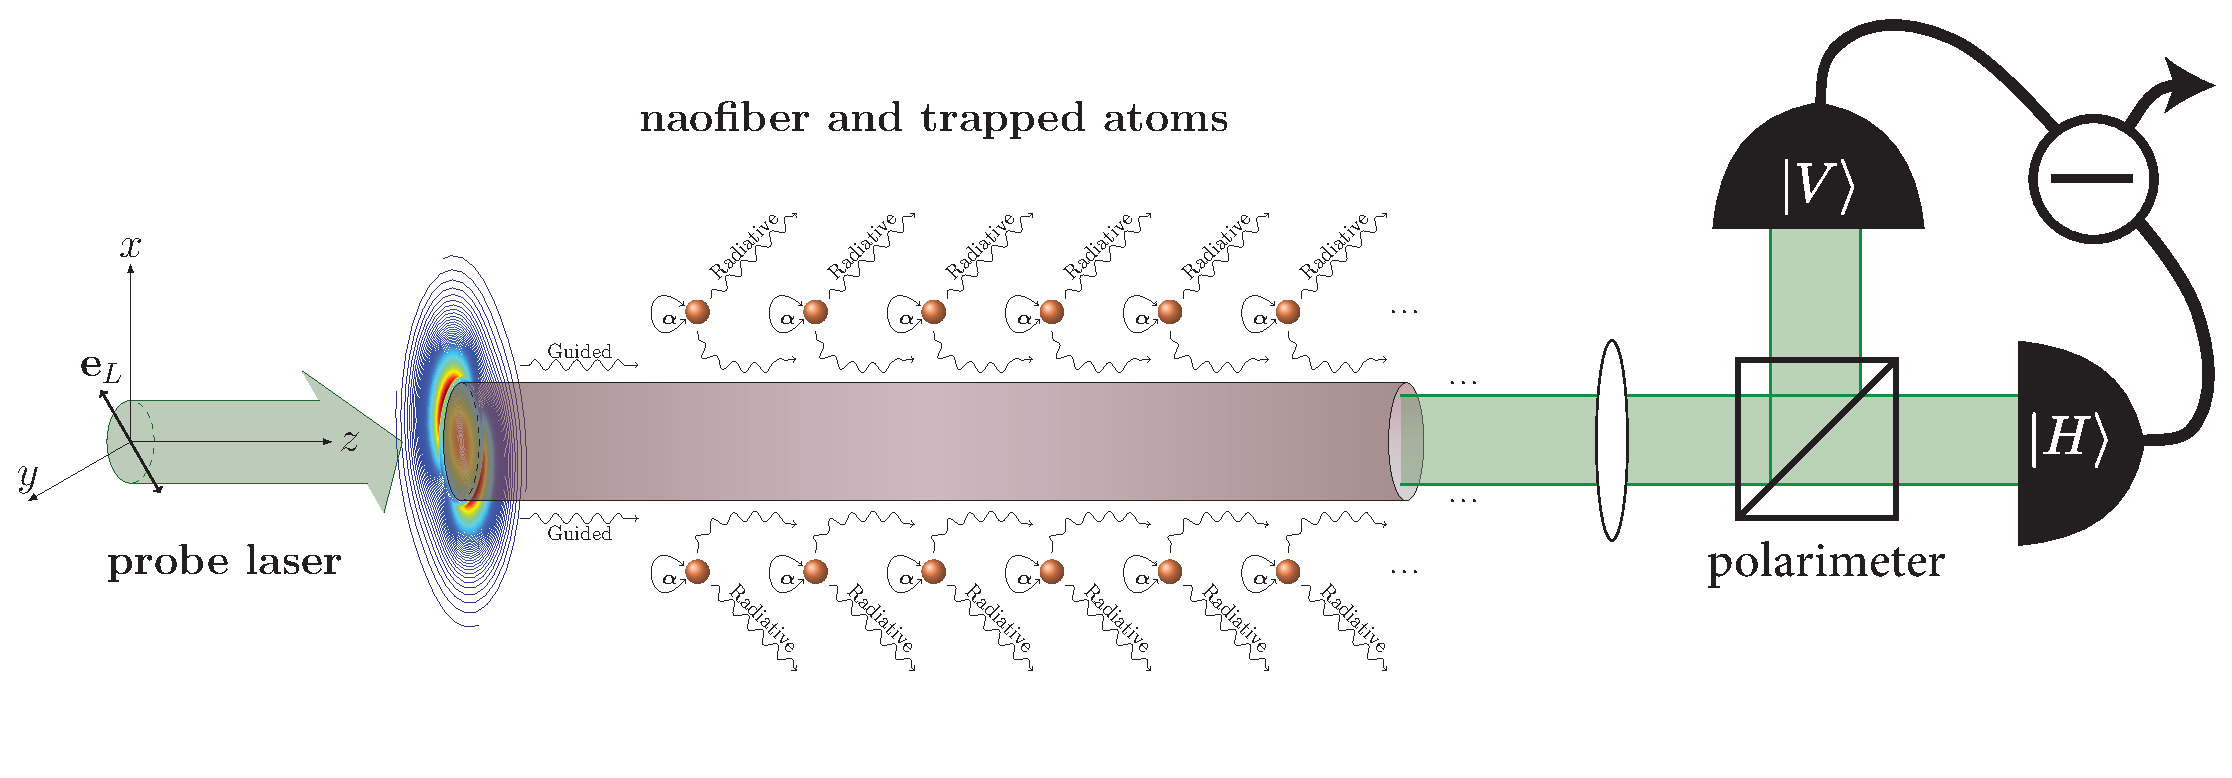
\includegraphics[width=12cm]{../media/Figs/BirefringenceMeasurement}}
\caption{Setup diagram for birefringence measurement.}
\end{figure}

\begin{figure}
\centering\makebox[\textwidth]{
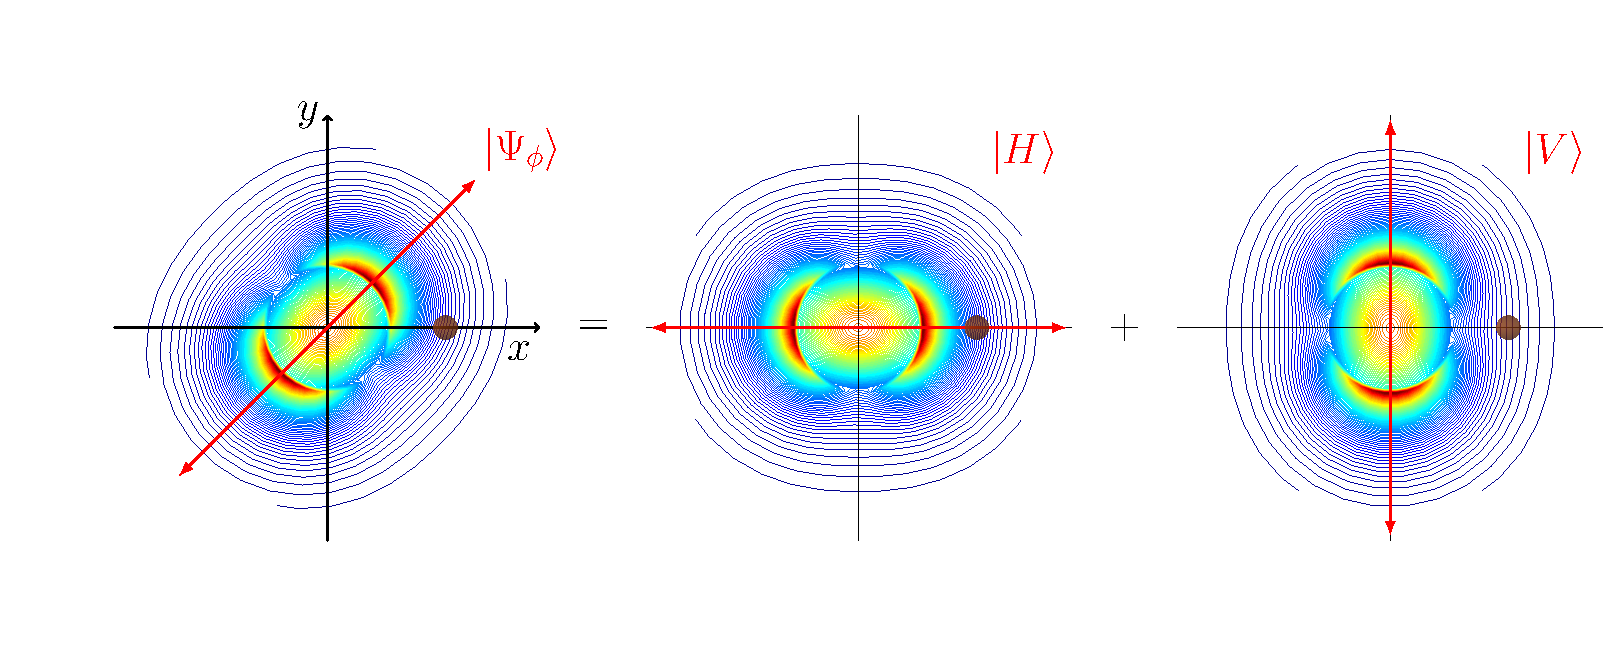
\includegraphics[width=12cm]{../media/Figs/Modes_Rot45HV}}
\caption[Mode decomposition of an input quasilinear polarized laser beam in the $ |H\rangle $ and $ |V\rangle $ mode basis.]{Mode decomposition of an input quasilinear polarized laser beam. The input beam is polarized along the bisection between $ x $- and $ y $-axes. It is equivalent to have one $ |H\rangle $ mode and one $ |V\rangle $ mode with input polarized along the $ x $-axis and $ y $-axis, respectively.}
\end{figure}

\begin{figure}
\centering\makebox[\textwidth]{
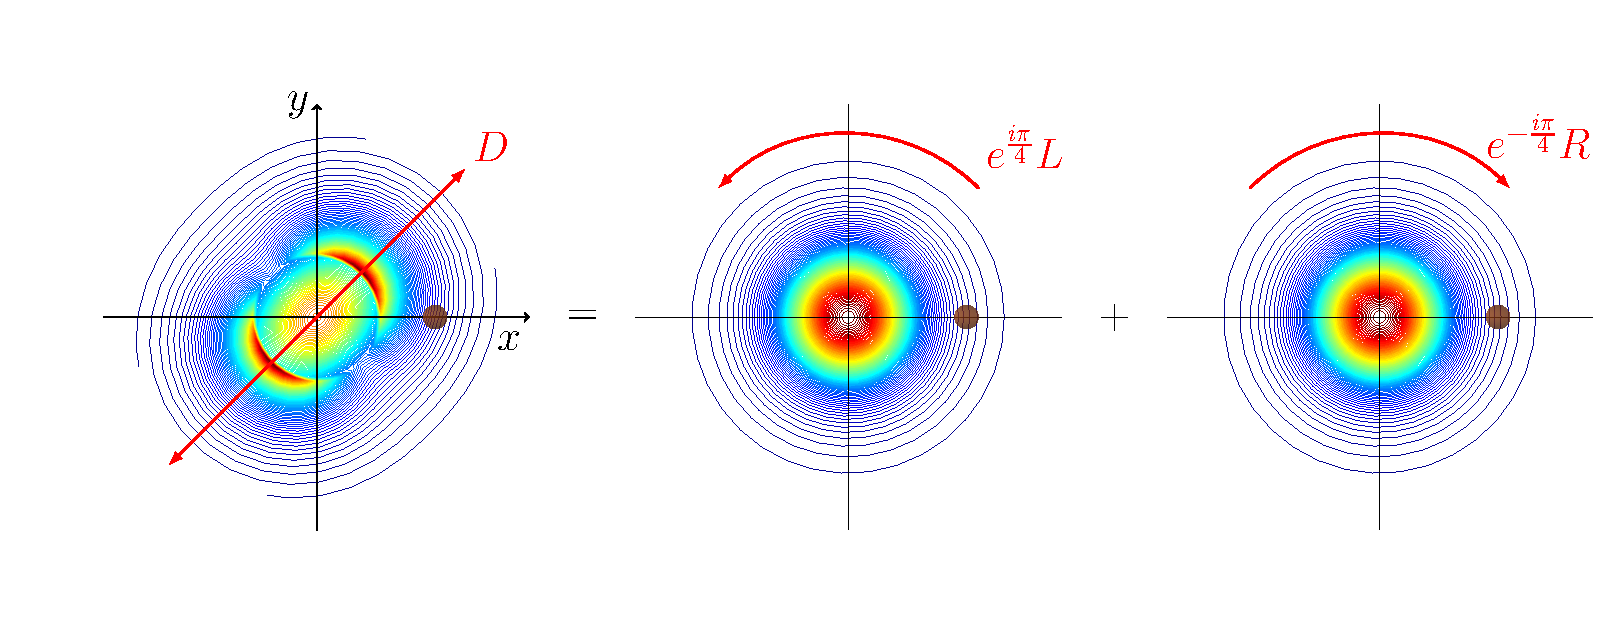
\includegraphics[width=12cm]{../media/Figs/Modes_Rot45LR}}
\caption[Mode decomposition of an input quasilinear polarized laser beam in the $ |L\rangle $ and $ |R\rangle $ mode basis.]{Mode decomposition of an input quasilinear polarized laser beam in the $ |L\rangle $ and $ |R\rangle $ mode basis. The input beam is polarized along the bisection between $ x $- and $ y $-axes. It is equivalent to have one $ |L\rangle $ mode and one $ |R\rangle $ mode with input circularly polarized light rotating counter-clockwise and clockwise, respectively.}
\end{figure}

\bigskip
\textbf{Comparison to the vacuum case:}

Notice that, the phase shift for an atom in vacuum can be given in a similar form by
\begin{align}
\delta\phi^{vac} &= 2\pi \frac{\omega_0}{cA} \Re[\alpha] |\mathbf{u}_{00}(\br')|^2 =  2\pi \frac{\omega_0}{c A^{vac'}_{e\!f\!f}} \Re[\alpha]=-\frac{1}{A} \sigma_0 |\mathbf{u}_{00} (r'_{\!\perp})|^2 \frac{\Gamma_{vac}}{4\Delta},
\end{align}
where $\mathbf{u}_{00}(\br')  $ is the TEM00 mode of a Gaussian laser field at the atom position, $ A=\frac{\pi W_0^2}{2} $ is the mode area of the Gaussian beam with wist $ W_0 $. Hence, the relative strength of phase shift due to the presence of a nanofiber versus vacuum can be given by
\begin{align}
\frac{\delta\phi^{nano}}{\delta\phi^{vac}} &=\frac{A_{e\!f\!f}^{vac'}}{A_{e\!f\!f}^{11}}= \frac{A}{2} \!n_g\! \frac{|\mathbf{u}_1(r_\perp^{nano'})|^2}{|\mathbf{u}_{00}(r_\perp^{vac'})|^2}.
\end{align}
In the vacuum case, the strongest mode is given by $ |\mathbf{u}_{00}(r_\perp^{vac'})|=1 $ when the atom is placed at the center of the beam waist. 



\section{Modification of the spontaneous emission of atoms trapped near a nanophotonic waveguide}

\comment{To be continued...}

\section{Resolution of birefringence spectroscopy measurement for the nanofiber trapped atom system}\label{sec:birefringenceresolution}
The Faraday spectroscopy theory for optical lattice has been published in Ref.~\cite{Smith2003a}. Following this thread, we present the birefringence spectroscopy analysis for our nanofiber case.

To measure the Stocks vector rotation angle on the \Poincare sphere, that is the transformation of the polarization of the light, we launch a probe light along the bisection line between $ x $- and $ y $-axes, and trap the atom on the $ x $-axis, and then measure the output powers of the counterclockwise-rotating ($ \sigma_+ $) and the clockwise-rotating ($ \sigma_- $) components of the output. From Equ.~\eqref{eq:Faradayrotang}, the total differential phase shift between the $ \sigma_+ $ and $ \sigma_- $ components of the probed traveling light interacted with $ N $ atoms can be given by
\begin{align}
\varphi_{_N} &= N\sigma_0\frac{c}{v_g}\frac{\Gamma_{vac}}{4\Delta}\left[| \mathbf{u}_H(r'_{\!\perp})|^2- | \mathbf{u}_V(r'_{\!\perp})|^2 \right].
\end{align}
\textcolor{red}{(Note: there may be a factor of 2 in the equation above and below. Needs to check.)}
The transformation of polarization is measured in terms of the total power difference between the $ x $- and $ y $-components of the field. The measured signal power is given by
\begin{align}
\Delta P_S &= P_0 \sin(\varphi_{_N}) \approx P_0 \varphi_{_N}. \label{eq:polsignal}
\end{align}

\textcolor{red}{Diagram of the experimental setup...}

Our resolution of detection is limited by the shot noise characterized by the fluctuations in the power difference with a root mean square amplitude of 
\begin{align}
\Delta P_{SN} &= \sqrt{\frac{P_0 \hbar \omega_0 }{2\kappa \tau_{pd}}}. \label{eq:shotnoise}
\end{align}
In the extreme case that the signal is equal to the noise, that is to make $ \Delta P_S=\Delta P_{SN} $, we can obtain the minimum number of atoms that we can detect (the resolution) as
\begin{align}
N_{min} &= \sqrt{\frac{8  \hbar \omega_0  }{P_0\kappa \tau_{pd}}}\frac{\Delta}{\sigma_0 n_g\Gamma_{vac}}\frac{1}{\left[| \mathbf{u}_H(r'_{\!\perp})|^2- | \mathbf{u}_V(r'_{\!\perp})|^2 \right]}\\
&=\sqrt{\frac{8  \hbar \omega_0  }{P_0\kappa \tau_{pd}}}\frac{2\pi\Delta}{3\lambda^2 \frac{4}{3} \left( \frac{\omega_0}{c}\right)^3 \frac{|d_{eg}|^2}{\hbar}}\frac{A_{e\!f\!f}^V}{\zeta -1 }\\
&= \sqrt{\frac{\hbar^3 \pi c  }{P_0\kappa \tau_{pd}\lambda}}\frac{\lambda\Delta }{  \left( 2\pi\right)^2 |d_{eg}|^2}\frac{A_{e\!f\!f}^V}{\zeta -1 }\\
&= \frac{1}{4\pi}\sqrt{\frac{\hbar^3 c \lambda }{\pi P_0\kappa \tau_{pd}}}\frac{\Delta }{   |d_{eg}|^2}\frac{A_{e\!f\!f}^V}{\zeta -1 },
\end{align}
with
\begin{align}
A_{e\!f\!f}^V &= \frac{1}{n_g| \mathbf{u}_V(r'_{\!\perp})|^2}\\
\zeta &= \frac{| \mathbf{u}_H(r'_{\!\perp})|^2}{| \mathbf{u}_V(r'_{\!\perp})|^2}.
\end{align}

\textbf{Estimating $ N_{min} $}:

We consider the critical time scale that 
\begin{align}
\tau_{pd} &= \frac{1}{\gamma_s},
\end{align}
where $ \gamma_{s} $ is the photon scattering rate. The minimum detectable atom number can be estimated using the relationship between the scattering rate and the scattering cross section $ \sigma(\Delta) $ or the saturation cross section $ \sigma_0 $ under the critical time scale. Now that
\begin{align}
\gamma_s &= \sigma(\Delta) \frac{I(\br')}{\hbar \omega_0} \\
\sigma(\Delta) &=\frac{\sigma_0}{1+\frac{4\Delta^2}{\Gamma^2_{vac}}}\approx \sigma_0 \frac{\Gamma_{vac}^2}{4\Delta^2} \quad \text{(far detuning.)}
\end{align}
Hence,
\begin{align}
\gamma_s &\approx \sigma_0\frac{\Gamma_{vac}^2}{4\Delta^2} \frac{I(\br')}{\hbar \omega_0}=\frac{\sigma_0}{A_{in}}\frac{P_0}{\hbar\omega_0}\frac{\Gamma_{vac}^2}{4\Delta^2},
\end{align}
where the effective incident mode area at the atom position, $A_{in}  $, is defined as
\begin{align}
A_{in }&= \frac{P_0}{I(\br')}.
\end{align}

We also treat the quantum efficiency $ \kappa=1 $. The critical shot noise defined in Eq.~\eqref{eq:shotnoise} then becomes
\begin{align}
\Delta P_{SN} &\approx \sqrt{\frac{P_0 \hbar \omega_0 \gamma_s}{2\kappa }} =P_0\sqrt{\frac{ \sigma_0 }{2A_{in}}}\frac{\Gamma_{vac}}{2\Delta}.
\end{align}
The signal defined in Equ.~\eqref{eq:polsignal} can be rewritten as
\begin{align}
\Delta P_S &= NP_0 \frac{\sigma_0}{A_{e\!f\!f}}\frac{\Gamma_{vac}}{4\Delta},
\end{align}
where the effective mode area at the atom position for our configuration is defined by
\begin{align}
A_{e\!f\!f} &= \frac{1}{n_g}\frac{1}{| \mathbf{u}_H(r'_{\!\perp})|^2- | \mathbf{u}_V(r'_{\!\perp})|^2}.
\end{align}
If we make the shot noise power equal to the minimum detectable signal power, we can obtain the minimum detectable atom number as
\begin{align}
N_{min} &= \sqrt{\frac{2A_{e\!f\!f}^2}{A_{in}\sigma_0}}.
\end{align}

\textcolor{red}{Compare to vacuum case?}


%</waveguideinterface>



\appendix
% ########################### Apendix ##########################################

%<*eigenmode>

\chapter{Fundamental eigenmodes of an optical nanofiber}
To simplify the problem of light scattering in a nanofiber trapped atoms system, we treat the atoms as a dipole oscillator moving in a classical electrical field $ \mathrm{E}_{g}(\br,t) $ guided along the nanofiber, and re-emit a scattered optical field described by $ \mathrm{E}^s(\br,t) $ to interfere with the initial guided optical field. Formally, the total optical field $ \mathrm{E}(\br,t)= \mathrm{E}^g(\br,t)  + \mathrm{E}^s(\br,t) $ implies a change of index of refraction and decoherence\index{decoherence} due to the presence of the atoms. 

In the case of a nanofiber with a sub-wavelength radius, the high-order modes of the nanofiber can hardly be supported, which only leaves over the HE11 mode\index{HE11 mode} propagating along the nanofiber. Assuming the incident light is quasi-linearly polarized, the Cartesian components of the bound optical field are given, for $ r_\perp>a $ (outside the fiber), by~\cite{Lacroute2012,LeKien2004}
\begin{subequations}
\label{Ertrga}
\begin{align}
E_x^g(r_\perp,\phi,z,t) &= iA \frac{\beta_{11}J_1(h_{11}a)}{2q_{11}K_1(q_{11}a)}[(1-s_{11})K_0(q_{11}r_\perp)\cos (\varphi_0) \nonumber\\
&\qquad + (1+s_{11})K_2 (q_{11}r_\perp) \cos (2\phi-\varphi_0) ] e^{-i(\omega t-f\beta_{11}z)},\\
E_y^g(r_\perp,\phi,z,t) &= iA \frac{\beta_{11}J_1(h_{11}a)}{2q_{11}K_1(q_{11}a)}[(1-s_{11})K_0(q_{11}r_\perp)\sin (\varphi_0) \nonumber\\
&\qquad + (1+s_{11})K_2 (q_{11}r_\perp) \sin (2\phi-\varphi_0) ] e^{-i(\omega t-f\beta_{11}z)},\\
E_z^g(r_\perp,\phi,z,t) &= fA \frac{J_1(h_{11}a)}{K_1(q_{11}a)}K_1(q_{11}r_\perp)\cos (\phi-\varphi_0) e^{-i(\omega t-f\beta_{11}z)},
\end{align}
\end{subequations}
and, for $ r_\perp<a $ (inside the nanofiber), by
\begin{subequations}
\label{Ertrla}
\begin{align}
E_x^g(r_\perp,\phi,z,t) &= iA \frac{\beta_{11}}{2h_{11}}[(1-s_{11})J_0(h_{11}r_\perp)\cos (\varphi_0) \nonumber\\
&\qquad - (1+s_{11})J_2 (h_{11}r_\perp) \cos (2\phi-\varphi_0) ] e^{-i(\omega t-f\beta_{11}z)},\\
E_y^g(r_\perp,\phi,z,t) &= iA \frac{\beta_{11}}{2h_{11}}[(1-s_{11})J_0(h_{11}r_\perp)\sin (\varphi_0) \nonumber\\
&\qquad - (1+s_{11})J_2 (h_{11}r_\perp) \sin (2\phi-\varphi_0) ] e^{-i(\omega t-f\beta_{11}z)},\\
E_z^g(r_\perp,\phi,z,t) &= fA J_1(h_{11}r)\cos (\phi-\varphi_0) e^{-i(\omega t-f\beta_{11}z)},
\end{align}
\end{subequations}
with
\begin{subequations}
\begin{align}
s_{11} &= \left[\frac{1}{(h_{11}a)^2}+ \frac{1}{(q_{11}a)^2} \right] \left[ \frac{J_1'(h_{11}a)}{h_{11}aJ_1(h_{11}a)} + \frac{K'_1(q_{11}a)}{q_{11}aK_1(q_{11}a)} \right],\\
h_{11} &= \sqrt{k_0^2 n_1^2-\beta_{11}^2},\\
q_{11} &= \sqrt{\beta^2_{11}-k_0^2 n_2^2}.
\end{align}
\end{subequations}
Here, $ k_0 $ is the vacuum wavenumber\index{wavevector!vacuum wavenumber} of the incident light; $ f=+,- $ indicates forward or backward propagation direction; $ \phi $ denotes the azimuthal angle in the transverse plane; $ \varphi_0 $ indicates the polarization axis for the incident polarization relative to the $ x  $ axis; $ n_1 $ and $ n_2 $ are the refractive indices\index{refractive index}\index{index of refraction} of inside and outside the nanofiber; $ \beta_{11} $ is the mode propagation constant; $ 1/h_{11} $ is the characteristic decay length for the bound mode inside the fiber; $ 1/q_{11} $ is the characteristic decay length outside the fiber; $ A $ is the real-valued amplitude for the linearly polarized input; $ J_l $ and $ K_l  $ are the $ l $th Bessel function of the first kind\index{Bessel function!Bessel function of the first kind} and the modified Bessel function of the second kind\index{Bessel function!modified Bessel function of the second kind}. As shown in Equs.~\ref{Ertrga} and~\ref{Ertrla}, we can factorize the $ \mathbf{E}^g(r_\perp,\phi,z,t) $ as $ \mathbf{E}^g(r_\perp,\phi,z,t)= \boldsymbol{\mathcal{E}}^g(\br)e^{i\omega t} $. 

Using the coordinate system transformation relationships that
\begin{align}
\hat{\br}\!_\perp &= \hat{\mathbf{x}}\cos\phi + \hat{\mathbf{y}}\sin\phi,\\
\hat{\phi} &= -\hat{\mathbf{x}}\sin\phi + \hat{\mathbf{y}}\cos\phi,
\end{align}
one can also express the transverse components of the electric field components in the polar coordinate, for $ r\!_\perp>a $, by
\begin{subequations}
\label{Erptlrga}
\begin{align}
E_{r\!_\perp}^g(r_\perp,\phi,z,t) &= iA \frac{\beta_{11}J_1(h_{11}a)}{2q_{11}K_1(q_{11}a)}[(1-s_{11})K_0(q_{11}r_\perp) \nonumber\\
&\qquad + (1+s_{11})K_2 (q_{11}r_\perp) ]\cos (\phi-\varphi_0) e^{-i(\omega t-f\beta_{11}z)},\\
E_\phi^g(r_\perp,\phi,z,t) &= -iA \frac{\beta_{11}J_1(h_{11}a)}{2q_{11}K_1(q_{11}a)}[(1-s_{11})K_0(q_{11}r_\perp) \nonumber\\
&\qquad - (1+s_{11})K_2 (q_{11}r_\perp) ]\sin (\phi-\varphi_0) e^{-i(\omega t-f\beta_{11}z)},
\end{align}
\end{subequations}
and, for $ r_\perp<a $, by
\begin{subequations}
\label{Ephirtlrla}
\begin{align}
E_{r\!_\perp}^g(r_\perp,\phi,z,t) &= iA \frac{\beta_{11}}{2h_{11}}[(1-s_{11})J_0(h_{11}r_\perp) \nonumber\\
&\qquad - (1+s_{11})J_2 (h_{11}r_\perp)  ]\cos (\phi-\varphi_0) e^{-i(\omega t-f\beta_{11}z)},\\
E_\phi^g(r_\perp,\phi,z,t) &= -iA \frac{\beta_{11}}{2h_{11}}[(1-s_{11})J_0(h_{11}r_\perp) \nonumber\\
&\qquad + (1+s_{11})J_2 (h_{11}r_\perp)  ]\sin (\phi-\varphi_0) e^{-i(\omega t-f\beta_{11}z)}.
\end{align}
\end{subequations}

Alternatively, we can use the fundamental mode with rotating polarization to decompose arbitrary polarized mode propagating in the fiber. The solutions for the cylindrical components of the circulating polarized fundamental mode are given~\cite{Lacroute2012,Vetsch2010a}, for $ r_\perp<a $, by
\begin{subequations}
\label{Ertcrla}
\begin{align}
E^{(\mu)}_{r_\perp}(r_\perp,\phi,z,t) &=iA\frac{\beta_{11}}{2h_{11}}e^{-i(\omega t-f\beta_{11} z -p\phi)}\nonumber\\
&\qquad \left[ (1-s_{11})J_0(h_{11}r_\perp)-(1+s_{11})J_2(h_{11}r_\perp) \right]\\
E^{(\mu)}_\phi(r_\perp,\phi,z,t) &=  -pA \frac{\beta_{11}}{2h_{11}}e^{-i(\omega t-f\beta_{11} z -p\phi)} \nonumber\\
&\qquad \left[ (1-s_{11})J_0(h_{11}r_\perp) +(1+s_{11})J_2(h_{11}r_\perp) \right] \\
E^{(\mu)}_z(r_\perp,\phi,z,t) &= fA J_1(h_{11}r_\perp) e^{-i(\omega t-f\beta_{11} z -p\phi)},
\end{align}
\end{subequations}
and, for $ r_\perp>a $, by
\begin{subequations}
\label{Ertcrga}
\begin{align}
E^{(\mu)}_{r_\perp}(r_\perp,\phi,z,t) &=iA\frac{\beta_{11}}{2h_{11}}\frac{J_1(h_{11}a)}{K_1(q_{11}a)}e^{-i(\omega t-f\beta_{11} z -p\phi)} \nonumber\\ 
&\qquad \left[ (1-s_{11})K_0(q_{11}r_\perp)+(1+s_{11})K_2(q_{11}r_\perp) \right]\\
E^{(\mu)}_\phi(r_\perp,\phi,z,t) &=  -pA \frac{\beta_{11}}{2h_{11}} \frac{J_1(h_{11}a)}{K_1(q_{11}a)}e^{-i(\omega t-f\beta_{11} z -p\phi)} \nonumber\\ 
&\qquad \left[ (1-s_{11})K_0(q_{11}r_\perp) - (1+s_{11})K_2(q_{11}r_\perp) \right] \\
E^{(\mu)}_z(r_\perp,\phi,z,t) &= fA \frac{J_1(h_{11}a)}{K_1(q_{11}a)} K_1(q_{11}r_\perp) e^{-i(\omega t-f\beta_{11} z -p\phi)}.
\end{align}
\end{subequations}
In Equs.~\ref{Ertcrla} and~\ref{Ertcrga}, we denote the normalized bound fundamental modes as $ \mathbf{E}^{(\mu)} (\br,t)$ by an index $ \mu=(\omega,f,p) $, where $ f=+,- $ denotes forward or backward propagation direction, and $ p=+,- $ denotes the conterclockwise or clockwise of polarization. Similar to the qusi-linear case, we use $ \boldsymbol{\mathcal{E}}^{p=\pm} $ to indicate the spatial components of the field with a given circulation pattern. For a linearly polarized HE11 mode, the cylindrical components are just the superposition of the two circular fields, 
\begin{align}\label{Eilincyc}
E_i^{lin} = \frac{1}{\sqrt{2}}(E_i^+ + E_i^-)\quad \mathrm{or}\quad \mathcal{E}_i^{lin} = \frac{1}{\sqrt{2}}(\mathcal{E}_i^+ + \mathcal{E}_i^-),\quad i\in(r_\perp,\phi,z).
\end{align}

\subsection{Power flow and normalization factor $ A $}
As discussed in Vetsch's dissertation~\cite{Vetsch2010a}, the real-valued amplitude factor $ A $ can be calculated by normalizing the total power of the light propagating in the fiber via the Poynting vector\index{Poynting vector}
\begin{align}
\left<\mathbf{S}\right>=\frac{1}{2} \Re\left[\boldsymbol{\mathcal{E}}^g(\br)\times{\boldsymbol{\mathcal{H}}^g(\br)}^* \right],
\end{align}
where $ \boldsymbol{\mathcal{H}}^g(\br) $ is the magnetic field of the guided light. 
Since the $ z $-component of the Poynting vector\index{Poynting vector} $ \left< S_z\right> $ qualifies the energy flux of the electromagnetic field in the propagation direction, integrating $ \left< S_z \right> $ over the transverse plane leads to the power propagating inside and outside the fiber
\begin{align}
P_{in} &= \int_0^{2\pi} \mathrm{d}\phi \int_0^a \left< S_z \right> r_\perp \mathrm{d}r_\perp\\
P_{out} &= \int_0^{2\pi} \mathrm{d}\phi \int_a^\infty \left< S_z \right> r_\perp \mathrm{d}r_\perp.
\end{align}
Using the total transmission power $ P=P_{in}+P_{out} $, the normalization constant $ A $ reads
\begin{align}\label{eq:A}
A=\sqrt{\frac{4\mu_0\omega P}{\pi a^2 \beta_{11}}}\left(D_{in} + D_{out} \right)^{-1/2},
\end{align}
where
\begin{align}
D_{in} &= (1-s_{11})\left[ 1+(1-s_{11})\frac{\beta_{11}^2}{h_{11}^2}\right] \left(J_0^2(h_{11}a) + J_1^2(h_{11}a) \right) \nonumber\\
&\quad + (1+s_{11})\left[ 1+(1+s_{11})\frac{\beta_{11}^2}{h_{11}^2}\right] \left(J_2^2(h_{11}a)- J_1(h_{11}a)J_3(h_{11}a) \right)\\
D_{out} &= \frac{J_1^2(h_{11}a)}{K_1^2(q_{11}a)}\left\{ (1-s_{11})\left[ 1-(1-s_{11})\frac{\beta_{11}^2}{q_{11}^2}\right] \left(K_0^2(q_{11}a) - K_1^2(q_{11}a) \right)\right. \nonumber\\
&\quad \left. + (1\!+\! s_{11})\left[ 1\!-\! (1\!+\! s_{11})\frac{\beta_{11}^2}{q_{11}^2}\right] \left(K_2^2(q_{11}a)\! -\! K_1(q_{11}a)K_3(q_{11}a) \right) \right\}.
\end{align}
The ratio of $ D_{in} $ and $ D_{out} $ indicates the intensity distribution division inside and outside of the nanofiber. 

\subsection{Energy density and normalization factor for traveling field quantization}
The energy per unit length stored in the waveguide is defined as
\begin{align}
W &= \frac{1}{2} \int \mathrm{d}\br\!_\perp n^2(\br\!_\perp) |\boldsymbol{\mathcal{E}}^g(\br\!_\perp)|^2.
\end{align} 
In our case, we can reform the integral over the transverse plane into the inside of the nanofiber and outside of the nanofiber parts. That is to say
\begin{align}
\int \mathrm{d} \br\!_\perp &= \int_0^{2\pi}\!\!\!\! \mathrm{d} \phi \int_0^a\!\!r\!_\perp \mathrm{d}r\!_\perp + \int_0^{2\pi}\!\!\!\! \mathrm{d} \phi \int_a^\infty\!\!r\!_\perp \mathrm{d}r\!_\perp.
\end{align}
Hence, the energy stored per unit distance of propagation can be rewritten as 
\begin{align}
W &= n_1^2P_1+n_2^2P_2,
\end{align}
where the power flow or the intensity distribution factors $ P_1 $ and $ P_2 $ can be found by
\begin{align}
\!\!\!\!\! P_1 &= \int_0^{2\pi} \!\!\mathrm{d} \phi \int_0^a\!\!\mathrm{d}r\!_\perp r\!_\perp|\boldsymbol{\mathcal{E}}^g(\br\!_\perp)|^2\\
&= \frac{\beta^2}{4h^2}\!\left\{(1\!-\! s)^2\!\left[J_0^2(ha)\!+\! J_1^2(ha) \right] \!+\!(1\!+\!s)^2\!\left[J_2^2(ha)\!-\!J_1(ha)J_3(ha) \right]\right\}\nonumber\\
&\quad +\frac{1}{2}\left[J_1^2(ha)-J_0(ha)J_2(ha) \right] \\
\!\!\!\!\! P_2 &= \int_0^{2\pi} \!\!\mathrm{d} \phi \int_a^\infty\!\!\mathrm{d}r\!_\perp r\!_\perp|\boldsymbol{\mathcal{E}}^g(\br\!_\perp)|^2\\
&= \frac{\beta^2J_1^2(ha)}{4q^2K_1^2(qa)}\!\left\{\phantom{\frac{1}{1}}\!\!\!\!(1\!-\!s)^2\!\left[K_1^2(qa)\!-\!K_0^2(qa) \right]\right.\nonumber\\
&\quad\left. \!+(1\!+\!s)^2\!\!\left[K\!_1\!(qa)K\!_3\!(qa)\!-\! K_2^2\!(qa) \right]\!+\!\frac{2q^2}{\beta^2}\!\!\left[K\!_0\!(qa)K\!_2\!(qa)\!-\!K_1^2\!(qa) \right]  \right\}.
\end{align}

Also, to quantize the traveling field of waveguide modes, we can define the normalization factor to be~\cite{LeKien2005a}
\begin{align}
N_g &= \int_0^{2\pi} \!\!\mathrm{d} \phi \int_0^\infty\!\!\mathrm{d}r\!_\perp r\!_\perp\,  n^2(\br\!_\perp)|\boldsymbol{\mathcal{E}}^g(\br\!_\perp)|^2\\
&= 2\pi A^2 a^2 (n_1^2P_1 + n_2^2P_2),
\end{align}
where the factor $ A $ is defined in Equ.~\eqref{eq:A} related to the input power. The full expression of radiative modes of the nanofiber system can also be found in Ref.~\cite{LeKien2005a}.

For some cases, the total power $ P $ can also be defined as
\begin{align}
P &= \int \mathrm{d}\br\!_\perp \langle S(\br\!_\perp)\rangle =\int \mathrm{d} \br\!_\perp I(\br\!_\perp)=\frac{\varepsilon_0 c n_{e\!f\!f}}{2}\int |\boldsymbol{\mathcal{E}}^g(\br\!_\perp)|^2,
\end{align}
where $ n_{e\!f\!f} $ is the effective index of refraction of the waveguide. 
By plugging in the field expression from Equs.~\eqref{Ertcrla} and~\eqref{Ertcrga}, we find the effective index of refraction for the HE11 modes of the nanofiber can be given by
\begin{align}
n_{e\!f\!f} &=\frac{\int \mathrm{d}\br\!_\perp n^2(\br\!_\perp) |\boldsymbol{\mathcal{E}}^g(\br\!_\perp)|^2}{\int |\boldsymbol{\mathcal{E}}^g(\br\!_\perp)|^2}\\
&= \frac{n_1^2\int_0^{2\pi} \!\!\mathrm{d} \phi \int_0^a\!\!r\!_\perp\mathrm{d}r\!_\perp|\boldsymbol{\mathcal{E}}^g(\br\!_\perp)|^2 + n_2^2\int_0^{2\pi}\!\! \mathrm{d} \phi \int_a^\infty\!\!r\!_\perp \mathrm{d}r\!_\perp|\boldsymbol{\mathcal{E}}^g(\br\!_\perp)|^2}
{\int_0^{2\pi} \!\!\mathrm{d} \phi \int_0^a\!\!r\!_\perp\mathrm{d}r\!_\perp|\boldsymbol{\mathcal{E}}^g(\br\!_\perp)|^2 + \int_0^{2\pi}\!\! \mathrm{d} \phi \int_a^\infty\!\!r\!_\perp \mathrm{d}r\!_\perp|\boldsymbol{\mathcal{E}}^g(\br\!_\perp)|^2}\\
&= \frac{n_1^2P_1+n_2^2P_2}{P_1+P_2}.
\end{align}
Notice that, the group index of refraction is not the same as the $ n_{e\!f\!f} $ defined above. We will discuss group velocity and group index of refraction of a waveguide later. See also the notes on \textit{Group velocity of the nanofiber}. 

%</eigenmode>

%###################################################################################
\bibliographystyle{../styles/abbrv-alpha-letters-links}
\bibliography{../refs/Archive}
%%%%%%%%%%%%%%%%%%%%%%%%%%%%%%%%%%%%%%%%%%%%%%%%%%%%%%%%%%%%%%%%%%%%%%%%%%%%%%%%%%%%

\printindex
\end{document}


\ExecuteMetaData[../chap3/QuantumDynamics.tex]{quantumdynamics}
%\documentclass[fleqn, final]{../styles/unmphythesis}
\usepackage{../styles/qxd}
\renewcommand{\thechapter}{3}
%\newcommand{\thechapter}{1}

\makeindex
\begin{document}

%<*quantumdynamics>

\chapter[QND measurement and spin squeezing with photonic waveguides]{Quantum non-demolition measurement and spin squeezing with nanophotonic waveguides}\label{chap:quantumdynamicsrepresentation}
\section{Introduction}
In the last chapter, we have treated the light as a classical field. 
In this chapter, we will fully quantize the optical field and study the quantum noise origin of the light by redefining the Stokes operators using the bosonic operators, and introduce the Hamiltonian of the atom-light interaction for the quantum non-demolition (QND) measurement. We will also link the collective spin operators to the traditional squeezing operators and finally introduce the QND-measurement--induced spin squeezing. 

\section[Atom-light coupling with waveguide modes]{Atom-light coupling with waveguide modes}
We consider atoms are trapped on a one-side or two-side chain of optical lattice near a nanophotonic waveguide and a probe is launched to perform the quantum measurement using the polarization spectroscopy technique introduced in the last chapter. We assume all atoms are trapped at the same distance to the waveguide surface and have the same local intensity of the probe. Defects of occupations on the optical lattices are allowed in our theory, and the minimum distance between atoms is large enough that we can ignore the photon scattering effect among atoms in the dispersive regime. Experiments on implementing such an atom-waveguide quantum interface have been done with optical nanofibers~\cite{Goban2012,Lacroute2012,Vetsch2010Optical,Lee2015,Beguin2014,Bajcsy2011Laser}, integrated optical waveguide couplers~\cite{Lee2013} and photonic crystal waveguides~\cite{Yu2014,Goban2014}. The designs of general nanophotonic waveguides for feasible atomic traps and atom-light interaction experiments have also been proposed for a broader range of atom-waveguide interfaces~\cite{Muniz2015Designing,Hung2013,Lee2017Characterizations}. We focus on the waveguides that allows two orthogonally polarized forward-propagating guided modes with degenerate group index of refraction, $ n_g $. 

Given an input light that adiabatically connects to the forward-propagating quasi-monochromatic $ p $-mode at frequency $ \omega_0 $, we define the field operators $ \hat{a}^\dagger_p(z,t) $ by~\cite{Gardiner1985Input,Blow1990Continuum,LeKien2008}
	\begin{align}
		\hat{a}_{p}(z,t) =\frac{1}{\sqrt{2 \pi}}  \int_0^{\infty}\!\!\!\!\! d \omega \, \hat{a}_{p}(\omega) e^{i[\beta_0 z- (\omega-\omega_0) t ]}, 
	\end{align}
that satisfy the free-field commutation relations,
	\begin{equation} \label{Eq::InputOutputCommutation}
		\big[\hat{a}_{p}(z,t),\hat{a}^\dag_{p'}(z',t')\big]=\delta_{p,p'}  \delta(t-t'-(z-z')/v_g).
	\end{equation}
The corresponding positive-frequency electric field operators in the orthogonal mode basis can be defined as
	\begin{equation} \label{Eq::PropagatingElectricField_forward}
		\hat{\mathbf{E}}^{(+)}(r\!_\perp,\phi,z;t) = \sum_{p} \sqrt{ \frac{2 \pi \hbar \omega_0}{ v_g} } \mathbf{u}_{p}(r\!_\perp,\phi) \hat{a}_{p}(z,t)  e^{i \beta_0 z},
	\end{equation}	
where the sum over $ p $ includes all components of a complete mode basis. Below, we only consider the $ \{H,V \} $ mode basis. The transformation of operators to another arbitrary mode bases is derived in Appendix~\ref{chap:basistransfHS}. 
With $ N_A $ atoms interacting with the propagating electric field of the local guided modes, the dispersive light-shift Hamiltonian can be defined as~\cite{Deutsch2010a,LeKien2013,Baragiola2014Open},
	\begin{equation} \label{Eq::LightShiftHam_forward}
		\hat{H}_{LS} = \sum_{n=1}^{N_A} \hat{h}_{\rm eff},
	\end{equation}
with the light-atom interaction Hamiltonian with one atom given by
\begin{align}
\hat{h}_\eff &= -\hat{\mathbf{E}}^{(-)}(\br')\cdot\hat{\tensor{\mathbf{\alpha}}}\cdot\hat{\mathbf{E}}^{(+)}(\br')\nn\\
&= -\frac{2\pi\hbar\omega}{v_g}\left[\mathbf{u}_H^*\cdot\hat{\tensor{\mathbf{\alpha}}}\cdot \mathbf{u}_H\hat{a}_H^\dagger\hat{a}_H\right.
+ \mathbf{u}_H^*\cdot\hat{\tensor{\mathbf{\alpha}}}\cdot \mathbf{u}_V\hat{a}_H^\dagger\hat{a}_V\nn\\
&\quad\quad + \mathbf{u}_V^*\cdot\hat{\tensor{\mathbf{\alpha}}}\cdot \mathbf{u}_H\hat{a}_V^\dagger\hat{a}_H 
\left. + \mathbf{u}_V^*\cdot\hat{\tensor{\mathbf{\alpha}}}\cdot \mathbf{u}_V\hat{a}_V^\dagger\hat{a}_V\right]\\
&= \hbar\left[(\hat{\chi}_{HH}+\hat{\chi}_{VV})\hat{S}_0 + (\hat{\chi}_{HH}-\hat{\chi}_{VV})\hat{S}_1 \right.\nn\\
&\quad \quad\left. + (\hat{\chi}_{HV}+\hat{\chi}_{VH})\hat{S}_2 + i(\hat{\chi}_{HV}-\hat{\chi}_{VH})\hat{S}_3 \right]\\
%\hbar \left[\left(\chi_{RR\uparrow} + \chi_{RR\downarrow} +\chi_{LL\uparrow}+\chi_{LL\downarrow} \right)\hat{F}_0\hat{S}_0 \right.\nonumber\\
%&\quad+\left(\chi_{RR\uparrow} + \chi_{RR\downarrow} -\chi_{LL\uparrow}-\chi_{LL\downarrow} \right)\hat{F}_0\hat{S}_3\nonumber\\
%&\quad+\left(\chi_{RR\uparrow} + \chi_{LL\uparrow} -\chi_{RR\downarrow}-\chi_{LL\downarrow} \right)\hat{F}_3\hat{S}_0\nonumber\\
%&\quad+\left(\chi_{RR\uparrow} - \chi_{RR\downarrow} +\chi_{LL\downarrow}-\chi_{LL\uparrow} \right)\hat{F}_3\hat{S}_3\nonumber\\
%&\quad+i\left(\chi_{LR\uparrow} - \chi_{RL\uparrow} +\chi_{RL\downarrow}-\chi_{RL\downarrow} \right)\hat{F}_0\hat{S}_1\nonumber\\
%&\quad+\left(\chi_{RL\uparrow} + \chi_{LR\uparrow} +\chi_{RL\downarrow}+\chi_{LR\downarrow} \right)\hat{F}_0\hat{S}_2\nonumber\\
%&\quad+i\left(\chi_{LR\uparrow} - \chi_{RL\uparrow} +\chi_{RL\downarrow}-\chi_{LR\downarrow} \right)\hat{F}_3\hat{S}_1\nonumber\\
%&\quad+\left.\left(\chi_{LR\uparrow} + \chi_{RL\uparrow} -\chi_{LR\downarrow}-\chi_{RL\downarrow} \right)\hat{F}_3\hat{S}_2 \right]\\
&=\hbar\sum_{i=0}^3 \hat{\chi}_{i}\hat{S}_i\\
&=\hbar\sum_{i,j=0} \chi_{ij}\hat{f}_i\hat{S}_j,
\end{align}
where $\poltens$ is the atomic tensor polarizability operator, given in \erf{Eq::AtomicPolarizabilityF}, for each atom trapped near the waveguide surface at position $\mathbf{r}'_\perp$ in the transverse plane. We ignore here any effects of atomic motion and treat the atoms as localized at fixed positions in space. We have also defined $ \hat{S}_i $ as the Stokes vector operators of the light indicating its polarization. The vector Stokes operators that describe the polarization of the propagating fields in the quasilinear $HV$-basis are given as below:
\begin{subequations}\label{Eq::StokesComponents}
	\begin{align} 
		\hat{S}_1(t) & = \smallfrac{1}{2}\big[ \hat{a}^\dag_H(t) \hat{a}_H(t)-\hat{a}^\dag_V(t) \hat{a}_V(t) \big], \\
	 	\hat{S}_2(t) & = \smallfrac{1}{2}\big[ \hat{a}^\dag_H(t) \hat{a}_V(t)+\hat{a}^\dag_V(t) \hat{a}_H(t) \big], \\ 
		\hat{S}_3(t) & = \smallfrac{1}{2i}\big[ \hat{a}^\dag_H(t) \hat{a}_V(t) -\hat{a}^\dag_V(t) \hat{a}_H(t) \big],
	\end{align}
\end{subequations}
that satisfy equal-$z$ commutation relations following from \erf{Eq::InputOutputCommutation},
	\begin{equation} \label{Eq::StokesCommutation}
		\big[\hat{S}_i(t), \hat{S}_j(t')\big] =i \epsilon_{ijk} \delta(t-t')  \hat{S}_k(t).
	\end{equation}
These, along with the total photon flux operator,
	\begin{equation}
		\hat{S}_0(t) = \smallfrac{1}{2}\big[ \hat{a}^\dag_H(t) \hat{a}_H(t)+\hat{a}^\dag_V(t) \hat{a}_V(t) \big],
	\end{equation}
are the quantum version of the Stokes vectors defined in Eq.~\eqref{eq:S_intensitydiff}. 
We also define the mode-atom coupling operator
\begin{align}
\hat{\chi}_{pp'} 
&=-\frac{2\pi \omega}{v_g}\mathbf{u}_{p}^*(r'\!_\perp,\phi')\cdot \hat{\tensor{\alpha}}\cdot \mathbf{u}_{p'}(r'\!_\perp,\phi')\\
&= \sum_{f'} \frac{n_g\sigma_0}{4}\frac{\Gamma_{f'}}{\Delta_{ff'}+i\Gamma_{f'}/2}\cdot \left\{ C_{j'ff'}^{(0)}\mathbf{u}_p^*(r'\!_\perp)\cdot \mathbf{u}_{p'}(r'\!_\perp)\hat{\mathbbm{1}}\right.\nn\\
&\quad\quad +iC_{j'ff'}^{(1)}\left(\mathbf{u}_p^*(r'\!_\perp)\times\mathbf{u}_{p'}(r'\!_\perp) \right)\cdot \hat{\mathbf{f}} \nonumber\\
&\quad\quad\left. + C_{j'ff'}^{(2)}\sum_{i,j}\left[u^*_{p,i}u_{p',j}(\frac{\hat{f}_i\hat{f}_j+\hat{f}_j\hat{f}_i}{2}-\frac{\delta_{ij}}{3}\hat{\mathbf{f}}\cdot\hat{\mathbf{f}}) \right]\right\}
%&\left.+C_{jj'ff'}^{(2)}\left[\mathbf{u}_p^*(r'\!_\perp)\cdot \mathbf{u}_{p'}(r'\!_\perp)\left(\frac{f(f+1)}{6}-\frac{m^2}{2} \right)+\mathbf{u}_p^*(r'\!_\perp)\cdot (\hat{e}^*_{\tilde{z}}\hat{e}_{\tilde{z}})\cdot \mathbf{u}_{p'}(r'\!_\perp)\left(\frac{3m^2}{2}-\frac{f(f+1)}{2} \right) \right] \right\}
\label{eq:chippp}
\end{align}
with the horizontally(H)- and vertically(V)-linearly polarized guided modes, $ \mathbf{u}_p(r'\!_\perp) $, at the atom position $ \br'=(r'\!_\perp,\phi',z') $. 
$ \chi_{ij}=\tr[\hat{f}_i\hat{\chi}_j]/(2f+1) $ is the coupling strength between spin operator $ \hat{f}_i $ and Stokes operator $ \hat{S}_j $. 
For example, $ \chi_{33} $ is the coupling strength between $ \hat{f}_z $ and $ \hat{S}_3 $.
The coupling operator or Eq.\eqref{eq:chippp} includes three terms corresponding to scalar, vector and tensor interactions between atoms and the probe light which are proportional to $ C_{j'ff'}^{(K)} $ with $ K=0,\,1,\,2 $, respectively.
These terms may be vanished depending on the state of atoms and the polarization state of the probe defined for the atom-light interaction protocol.

\section{Some special states of an alkali atom}
\subsection{Clock states}

\subsection{Stretched states}


We also ignore the tensor coupling strength related to $ C_{jj'ff'}^{(2)} $ terms in Eq.\eqref{eq:chippp} as the tensor interaction strength ($ \sim 1/\Delta^2 $) is relatively small compared to the vector interaction strength ($ \sim 1/\Delta $)~\cite{Deutsch2010a}. 
For a nanofiber geometry, the Faraday interaction coupling strength is independent of the azimuthal position of the atoms and can be simplified as
\begin{align}
\chi_{33} &= -\sum_{f'}n_g\sigma_0\frac{\Gamma_0}{\Delta_{ff'}+i\Gamma_0/2}C_{jj'ff'}^{(1)}u_{r\!_\perp}(r'\!_\perp)u_\phi(r'\!_\perp)\\
&=\frac{\sigma_0}{A_F}\frac{\Gamma_0}{\Delta_F},
\end{align}
where the effective Faraday interaction mode area $ A_F=1/2n_g|u_{r\!_\perp}(r'\!_\perp)u_\phi(r\!_\perp)| $, and the effective detuning $ \Delta_F=\sum_{f'}\frac{-C_{j'ff'}^{(1)}}{\Delta_{ff'}} $.
The measurement strength is now defined as
\begin{align}
\kappa\equiv|\chi_{33}|^2\dot{N}_L=\frac{\sigma_0A_{in}}{A_F^2}\gamma_s,
\end{align}
where the characteristic photon scattering rate $ \gamma_s\equiv \frac{\Gamma_0\Omega^2}{4\Delta_F}=\frac{\sigma_0}{A_{in}}\frac{\Gamma_0^2}{4\Delta_F^2}\dot{N}_L $ and the effective mode area $ A_{in}=1/n_g|u_{\mathrm{in}}(\br'\!_\perp)|^2 $.
Now we can define the OD per atom for the Faraday interaction using SCS by
\begin{align}
\frac{\mathrm{OD}}{N_A} \equiv \frac{\kappa}{\gamma_s}=\frac{\sigma_0A_{in}}{A_F^2}.
\end{align}





\section{Polarization spectroscopy and quantum nondemolition measurement for alkali atoms}
\subsection{Clock states as the pseudo-spin states for polarimetry}~\footnote{See the NanofiberInterface note and the AFOSRProposal (2010) for related discussions.}
Now, we use the $ f=3,\,m=0 $ and $ f=4,\,m=0 $ two sublevels of $ 6S_{1/2} $ ground state as the psuedo-spin to represent qubit. That is to say, $ \ket{\uparrow}=\ket{f=4,\,m=m_x=0} $ and $ \ket{\downarrow}=\ket{f=3,\,m=m_x=0} $, where we choose the $ x $ axis as the quantization axis. We also launch two orthogonal probe beams notated as mode $ H $ and mode $ V $, whose polarization axes are parallel or perpendicular to the $ x $ axis where the atom is lying in. We can quantize the propagating guided fields with duration $ \tau $ and photon number $ N_L $ as
\begin{align} \label{Eq::FiberModeFunctions}
		\hat{\mathbf{E}}^{(+)}(r\!_\perp,\phi,z) = \sqrt{ \frac{2 \pi \hbar \omega_0}{ v_g \tau} } \big( \mathbf{u}_H(r\!_\perp,\phi) \hat{a}_H + \mathbf{u}_V(r\!_\perp,\phi) \hat{a}_V \big) e^{i \beta z}.
\end{align}
\textcolor{red}{Note: We only consider the forward-propagating fields. Otherwise, it will mess up our results below.}

We are interested in developing a dispersive, state-dependent interface between the collective spin of these atoms and the guided field modes of the fiber.  We first consider the light-shift interaction for a single alkali atom interacting with detuned light in the guided modes of the tapered nanofiber.  Such an interaction is described by the effective Hamiltonian,
\begin{align}  \label{Eq::LightShiftHam}
	H_{\rm eff}   &= -\hat{\mathbf{E}}^{(-)}(r^\prime\!\!_\perp,\phi',z')\cdot \tensor{\alpha}\cdot \hat{\mathbf{E}}^{(+)}(r^\prime\!\!_\perp,\phi',z')\\
	&= -\frac{2\pi \hbar \omega_0}{ v_g\tau} \Big( \mathbf{u}^*_H(r^\prime\!\!_\perp, \phi')\! \cdot\! \tensor{\alpha}\! \cdot\! \mathbf{u}_{H}(r^\prime\!\!_\perp, \phi') \hat{a}\dg_H \hat{a}_H \nonumber\\
	&\quad\quad\quad\quad\quad +  \mathbf{u}^*_V(r^\prime\!\!_\perp, \phi') \!\cdot\! \tensor{\alpha}\! \cdot\! \mathbf{u}_{V}(r^\prime\!\!_\perp, \phi') \hat{a}\dg_V \hat{a}_V \\
	&\quad\quad\quad\quad\quad + \mathbf{u}^*_H(r^\prime\!\!_\perp, \phi') \!\cdot\! \tensor{\alpha}\! \cdot\! \mathbf{u}_{V}(r^\prime\!\!_\perp, \phi') \hat{a}\dg_H \hat{a}_V \nonumber\\
	&\quad\quad\quad\quad\quad + \mathbf{u}^*_V(r^\prime\!\!_\perp, \phi') \!\cdot\! \tensor{\alpha}\! \cdot\! \mathbf{u}_{H}(r^\prime\!\!_\perp, \phi') \hat{a}\dg_V \hat{a}_H \Big), \nonumber 
\end{align}
where the atom is positioned at $ (r^\prime\!\!_\perp,\phi',z') $. 
In the expansion above, the first two terms lead to the \emph{birefringent}\index{birefringence effect} coupling due to the different phase shifts between $ H $ and $ V $ modes. The second two terms lead to the \emph{Faraday}\index{Faraday effect!Faraday coupling} coupling due to a coherent redistribution of photons between $ H $ and $ V $ modes. The polarization dependence of the atom-probe coupling arises from two sources: the tensor nature of $ \tensor{\alpha} $ and the spatial dependence of $ \mathbf{u}_{H}(r\!_\perp, \phi) $ versus $ \mathbf{u}_{V}(r\!_\perp, \phi) $. The amplitude of the $ H $ mode is roughly $ 3 $ times larger than the $ V $ mode on the $ x $ axis. However, in the expression of the Hamiltonian there is always the atomic polarizability multiplied with the modes, which makes it a state-dependent problem. 

Note: alternatively, the effective Hamiltonian can also be rewritten using the irreducible tensor components as
\begin{align}  
H_{\rm eff} &= - \sum_{f,f'}\alpha_0(\Delta_{f,f'}) \left\{ C_{j'ff}^{(0)} \hat{\mathbf{E}}^{(-)} \cdot \hat{\mathbf{E}}^{(+)} \hat{\mathbbm{1}}_f \phantom{\frac{\hat{1}}{1}}\right. \nonumber\\
&\quad\quad\quad + i C_{j'ff'}^{(1)} \left(\hat{\mathbf{E}}^{(-)} \times \hat{\mathbf{E}}^{(+)} \right) \cdot \hat{ \mathbf{f}} \nonumber\\
&\quad\quad\quad  \left. + C_{j'ff}^{(2)} \hat{E}_i^{(-)} \hat{E}_j^{(+)} \left( \frac{ \hat{f}_i \hat{f}_j  + \hat{f}_j \hat{f}_i  }{2} - \frac{1}{3}\delta_{ij} \hat{ \mathbf{f}} \cdot \hat{\mathbf{f}}  \right) \right\}. \label{Eq::LightShiftHam_irep}
\end{align} 

In the weak excitation regime, we limit our attention to the clock state subspace, and hence the polarizability is restricted to the reduced tensor $ \bra{f,m=0}\tensor{\alpha}\ket{f,m=0}$, $f=3,4 $. We can denote such reduced atomic polarizability tensors as 
\begin{align}
\tensor{\alpha}_{\uparrow} &=\bra{f=4,m=0}\tensor{\alpha}\ket{f=4,m=0}\\
\tensor{\alpha}_{\downarrow} &=\bra{f=3,m=0}\tensor{\alpha}\ket{f=3,m=0}.
\end{align}


In the clock state subspace, the vector component of the atomic polarizability is always zeros due to the symmetry of quantum jumps. In the light-shift Hamiltonian expression (Equ.~\eqref{Eq::LightShiftHam}), the crossing terms involving products between both $ H $ and $ V $ modes vanish. 

Now that, the light shift Hamiltonian can be written as 
\begin{align}
H_{\rm eff} & = \frac{ \hbar }{ \tau}\Big( \chi_{H,\uparrow}\op{\uparrow}{\uparrow} +  \chi_{H,\downarrow} \op{\downarrow}{\downarrow} \Big) \hat{a}_H\dg \hat{a}_H \nonumber\\
&\quad +  \frac{ \hbar }{ \tau} \Big( \chi_{V,\uparrow}\op{\uparrow}{\uparrow} +  \chi_{V,\downarrow} \op{\downarrow}{\downarrow} \Big) \hat{a}_V\dg \hat{a}_V  \label{HeffLS}
\end{align}
where the single atom light shifts per photon or the coupling strengths for the different combination of clock states and polarizations are defined as
\begin{align}
\chi_{H,\uparrow} &=  -\frac{2\pi\omega_0}{v_g} \mathbf{u}^*_{H}(r^\prime\!\!_\perp,\phi') \cdot\tensor{\alpha}_{\uparrow}\cdot \mathbf{u}_{H}(r^\prime\!\!_\perp,\phi') \\
\chi_{H,\downarrow} &=  -\frac{2\pi\omega_0}{v_g} \mathbf{u}^*_{H}(r^\prime\!\!_\perp,\phi') \cdot\tensor{\alpha}_{\downarrow}\cdot \mathbf{u}_{H}(r^\prime\!\!_\perp,\phi') \\
\chi_{V,\uparrow} &=  -\frac{2\pi\omega_0}{v_g}  \mathbf{u}^*_{V}(r^\prime\!\!_\perp,\phi') \cdot\tensor{\alpha}_{\uparrow}\cdot \mathbf{u}_{V}(r^\prime\!\!_\perp,\phi')  \\
\chi_{V,\downarrow} &=  -\frac{2\pi\omega_0}{v_g}  \mathbf{u}^*_{V}(r^\prime\!\!_\perp,\phi') \cdot\tensor{\alpha}_{\downarrow}\cdot \mathbf{u}_{V}(r^\prime\!\!_\perp,\phi'). 
\end{align}

Suppose the probe laser is in a near resonance regime of the lower frequency side of the $ D_1 $ line so that the detuning from the ground $ 6S_{1/2} $ $ \ket{f=4} $ hyperfine level to the excited $ 6P_{1/2} $ $ \ket{f=3} $ hyperfine level is far greater than the hyperfine structure splitting of the excited states. We can then ignore the tensor component and the imaginary part of the atomic polarizability, as well as the higher level of excited states above the $ 6P_{1/2} $ energy levels. Baring that the vector component of the polarizability for the clock state vanishes, we only have the scalar coefficient $C_{j' f}^{(0)} =1/3  $ (from Equ.~\eqref{Eq::ScalarCoefSum}) non-zero.~\footnote{Similar case for the $ D_2 $ line will lead to $ C_{j' f}^{(0)} =2/3 $.} Therefore, the atomic polarizability can be given by
\begin{align}
\tensor{\alpha}_{\uparrow} &\approx\sum_{f'=3,4}\frac{\alpha_0(\Delta_{4,f'})}{3}\mathbbm{1} \\
\tensor{\alpha}_{\downarrow} &\approx\sum_{f'=3,4}\frac{\alpha_0(\Delta_{3,f'})}{3}\mathbbm{1},
\end{align}
with $ \alpha_0(\Delta_{f,f'})=-\frac{3\lambda_{j'j}^3}{32\pi^3} \frac{\Gamma}{\Delta_{f,f'}} $. In our case, we can make $ \lambda_{j'j}\approx\lambda= \frac{2\pi c}{\omega_0}$. Therefore, we have
\begin{align}
\frac{2\pi\omega_0}{v_g}\alpha_0(\Delta_{f,f'})=-\frac{n_g\sigma_0}{4} \frac{\Gamma}{\Delta_{f,f'}}
\end{align}
with the 3D atomic scattering cross section $ \sigma_0= \frac{3\lambda^2}{2\pi}  $. 

The coupling strength for the $ D_1 $ line probing can then be written as
\begin{align}
\chi_{H,\uparrow} &=   \frac{1}{2} \sum_{f'} \chi_{H0}(f',4) C_{j',f',4}^{(0)}  =  \frac{1}{2} \sum_{f'} \frac{\chi_{H0}(f',4)}{3} \label{chiHUp}  \\
\chi_{H,\downarrow} &=   \frac{1}{2} \sum_{f'} \chi_{H0}(f',3)  C_{j',f',3}^{(0)} = \frac{1}{2} \sum_{f'} \frac{\chi_{H0}(f',3) }{3} \label{chiHDown}\\
\chi_{V,\uparrow} &=   \frac{1}{2} \sum_{f'} \chi_{V0}(f',4)  C_{j',f',4}^{(0)}  =   \frac{1}{2} \sum_{f'} \frac{\chi_{V0}(f',4)}{3}\label{chiVUp}  \\
\chi_{V,\downarrow} &=   \frac{1}{2} \sum_{f'} \chi_{V0}(f',3)  C_{j',f',3}^{(0)}=   \frac{1}{2} \sum_{f'} \frac{\chi_{V0}(f',3) }{3} \label{chiVDown}
\end{align}
and 
\begin{align}
\chi_{H0}(f',f) &= \left( \frac{ \sigma_0}{A_{ef\!f}^H} \right) \left( \frac{\Gamma}{2 \Delta_{f,f'}} \right)\\
\chi_{V0}(f',f) &= \left( \frac{ \sigma_0}{A_{ef\!f}^V} \right) \left( \frac{\Gamma}{2 \Delta_{f,f'}} \right)\\
A_{ef\!f}^H &= \frac{1}{n_g|\mathbf{u}_{H}(r^\prime\!\!_\perp,\phi')|^2}\\
A_{ef\!f}^V &= \frac{1}{n_g | \mathbf{u}_{V}(r^\prime\!\!_\perp,\phi')|^2}.\label{eq:AeffV}
\end{align}
Considering the relationship between $ \Gamma_{1D} $ and $ \Gamma_{vac} $ (the same as the $ \Gamma $ above) from Equ.~\eqref{Gamma1DGammavac}, Equs.~\eqref{chiHUp} and~\eqref{chiHDown} are equivalent to Equ.~\eqref{phaseshiftGamma1D} derived from the Green's function method with scalar polarizability. The scalar polarizability factor of $ C_{j',f',f}^{(0)}=\frac{1}{3} $ in Equ.~\eqref{chiHUp} through Equ.~\eqref{chiVDown} indicates the possibility of transitions back to the clock state. This factor can be absorbed into the atomic scattering cross section by treating the scattering cross section as an average over all possible quantum transitions. 

\subsection{Full Hamiltonian using Clebsch-Gordan coefficients}
We can also work in the time-domain to include the wave-propagation process much carefully. \textcolor{red}{Note: part of the content below is directly from Ben's notes.}

For the nanofiber interface, we specify to the single-mode condition that only the HE$_{11}$ spatial mode propagates in the fiber with propagation constant $\beta_0$.  We can further make the first Markov approximation that the coupling is dominated by frequencies near an atomic transition frequency $\omega_0$ and then extend the limit of integration to $-\infty$ as a mathematical convenience.  We then define Fourier-transformed \emph{input-output field operators} that describe propagating modes in the nanofiber,
	\begin{align}
		\hat{a}_{\mu}(z,t) \equiv \frac{1}{\sqrt{2\pi}} \int_{-\infty}^{\infty} \mathrm{d}\omega \hat{a}_{\mu}(\omega) e^{i f \beta_0 z -i\omega_0 t}.
	\end{align}	
They satisfy the white-noise commutation relations
	\begin{align}
		[\hat{a}_{\mu}(z,t), \hat{a}\dg_{\mu'}(z',t')] = \delta_{p,p'} \delta_{f,f'} \delta(t-t' - |z-z'|/v_p).
	\end{align}	
Note that the commutation relation is related to the \emph{phase retarded time} which is related to the phase velocity, $v_p = \omega_0/\beta_0$, rather than the group velocity.  More details on this can be found in several of Le Kien's papers, including \emph{Correlations between photons emitted by multi-atom fluorescence into a nanofiber} (http://journals.aps.org/pra/pdf/10.1103/PhysRevA.77.033826).

The guided-mode electric field operator can then be written in terms of the input-output field operators
	\begin{align}\label{eq:Ebp}
		\hat{\mathbf{E}}_g^{(+)}(\mathbf{r}) = \sum_{f ,p} \sqrt{\frac{2 \pi \hbar \omega_0}{v_g}} \hat{a}_{\mu}(z,t) \mathbf{u}_{\mu}(\mathbf{r}_\perp) 
	\end{align}
We have dropped the $\omega(\beta)$ label on the mode functions as it is only for the fundamental propagation constant $\beta_0$.

Atoms can be trapped around the surface of the nanofiber using a handful of techniques.  In the interaction Hamiltonian $z=z' =z_A$ for the two field operators that appear, so we drop the $z$ label on the field operators $\hat{a}(z,t) \rightarrow \hat{a}(t)$.  This will not in general be valid when calculating the output propagating field operators, as their interaction will depend on the positions of the multiple atoms throughout the ensemble.  However, we make the assumption that the transit time through the nanofiber region is short compared to the collective atomic dynamics, and thus we can ignore the retarded group time.  

From Equ.~\eqref{Eq::LightShiftHam}, the effective Hamiltonian of the light-atom interaction at time $ t $ can then be given by
\begin{align}  
	H_{\rm eff}   = -\frac{2\pi \hbar \omega_0}{ v_g } &\Big( \mathbf{u}^*_H(r^\prime\!_\perp, \phi') 
	\!\cdot\! 
	\tensor{\alpha} \!\cdot\! \mathbf{u}_{H}(r^\prime\!_\perp, \phi') \hat{a}\dg_H(t) \hat{a}_H(t) \nonumber\\
	&\!\! +  
	\mathbf{u}^*_V(r^\prime\!_\perp, \phi')\! \cdot\! 
	\tensor{\alpha} \!\cdot\! \mathbf{u}_{V}(r^\prime\!_\perp, \phi') \hat{a}\dg_V(t) \hat{a}_V(t) \nonumber\\
	&\!\! + \mathbf{u}^*_H(r^\prime\!_\perp, \phi')\! \cdot\! \tensor{\alpha}\! \cdot\! 
	\mathbf{u}_{V}(r^\prime\!_\perp, \phi') \hat{a}\dg_H(t) \hat{a}_V(t) \nonumber\\
	&\!\! + \mathbf{u}^*_V(r^\prime\!_\perp, \phi') \!\cdot\! \tensor{\alpha}\! \cdot\! 
	\mathbf{u}_{H}(r^\prime\!_\perp, 
	\phi') \hat{a}\dg_V(t) \hat{a}_H(t) 
	\Big).  \label{eq:LightShiftHam_CG}
\end{align}
The atomic polarizability tensor $\tensor{\alpha}$\index{polarizability!polarizability tensor} is composed of a dyad of vector dipole operators,    
\begin{align}
	\tensor{\alpha} & =  - \frac{1}{\hbar}  \sum_{F,F'} \frac{ \mathbf{d}_{FF'} \mathbf{d}^\dagger_{F'F} 
	}{\Delta_{FF'}+i\frac{\Gamma}{2} } \\
		& = \sum_{q,q'}  \sum_{F,F'} \sum_{m_1, m_2, m'} \!\!\!\!\!\! \alpha_0(F,F') \mathbf{e}_q \otimes 
		\mathbf{e}^*_{q'} | o^{J'F'}_{JF} |^2 C^{Fm_2;1q}_{F'm'} C^{Fm_1;1q'}_{F'm'} \op{F m_2}{F m_1},
\end{align}
with the vector raising  dipole operator,
\begin{align}
	\mathbf{d}^\dagger_{F'F} =  \bra{P_{J'}}| d |\ket{S_{1/2}} \sum_q \sum_{m,m'} \mathbf{e}_q^* 
	o^{J'F'}_{JF} C^{Fm;1q}_{F'm'} \op{F'm'}{Fm}
\end{align}
where $o^{J'F'}_{JF}$ is the oscillator strength from Ref. \cite{Deutsch2010a} and $C^{Fm;1q}_{F'm'} 
\equiv 
\ip{F'm'}{Fm;1q}$ is a Clebsch-Gordan coefficient. 
Notice that $m' = m_1 + q'$ and $m' = m_2 + q$ and thus
\begin{align}
	m_2 - m_1 = q-q'.
\end{align}
The characteristic polarizability\index{polarizability!characteristic polarizability} is
\begin{align} \label{eq:CharacteristicPolarizability}
	\alpha_0(F,F') = - \frac{ |\bra{P_{J'}}| d |\ket{S_{1/2}}|^2 }{\hbar (\Delta_{F,F'}+i\frac{\Gamma}{2})} = - 
	\frac{3 
	\lambda_{J'}^3}{32 \pi^3} \frac{\Gamma}{\Delta_{F,F'}+i\frac{\Gamma}{2}}.
\end{align}
and the detuning is defined as
\begin{align}
	\Delta_{FF'} \equiv \omega - (\omega_{F'} - \omega_{F}).
\end{align}
Due to the hyperfine ground splitting in Cs$^{133}$ of approximately 9.2 GHz, the characteristic 
polarizabilities for the two ground hyperfine manifolds, \erf{eq:CharacteristicPolarizability}, can in 
general have different magnitudes and signs.  Implied in the expression above is that we have chosen a 
$J'$ transition - generally $S_{1/2} \rightarrow P_{1/2}$ ($D_1$) or $S_{1/2} \rightarrow P_{3/2}$ ($D_2$), 
which are 
separated by tens of THz and thus quite resolvable.   

Now suppose that rather than using the magnetic sublevels within a single ground hyperfine state $F$ as 
in Ref.~\cite{Deutsch2010a}, we begin with a dispersive interface defined on the $m=0$ ``\emph{clock}" states 
between the $F=3$ and $F=4$ hyperfine states.  To first order such states are insensitive to ambient 
magnetic field fluctuations.  In the clock-state subspace, we designate the qubit states
\begin{align} 
	\ket{\uparrow} &\equiv \ket{F = 4,m_F = 0} \\
 	\ket{\downarrow} &\equiv \ket{F = 3,m_F=0}.
\end{align}
The light shift Hamiltonian, \erf{eq:LightShiftHam_CG}, can then be expressed in this basis by finding 
the 
matrix elements between our relevant states.  Since the atomic polarizability tensor is block-diagonal in 
the ground hyperfine states, we need only consider coupling between the states within the same 
manifold.  
For instance, we may have a $H-V$ mode crossing term like
\begin{align} \label{eq:ClockMatrixElement}
	&\bra{F,0} \mathbf{u}^*_H(r^\prime\!_\perp, \phi') \cdot \tensor{\alpha} \cdot 
	\mathbf{u}_{V}(r^\prime\!_\perp, \phi') \ket{F,0}\nonumber\\
  =& 
	\sum_{F'} \sum_{m'} \sum_{q, q'} \alpha_0(F,F') \big( \mathbf{e}_q \cdot 
	\mathbf{u}^*_H(r^\prime\!_\perp, \phi') \big) 
	\big( \mathbf{e}^*_{q'} \cdot \mathbf{u}_V(r^\prime\!_\perp, \phi') \big) |o^{J'F'}_{JF} |^2 C^{F 0;1 
	q}_{F' m'} C^{F 
	0;1q'}_{F' m'} \\
 = & \sum_{F'} \sum_{q} \alpha_0(F,F') \big( \mathbf{e}_q \cdot \mathbf{u}^*_H(r^\prime\!_\perp, \phi') 
	\big) \big( 
	\mathbf{e}^*_{q} \cdot \mathbf{u}_V(r^\prime\!_\perp, \phi') \big) |o^{J'F'}_{JF} |^2 C^{F 0;1q}_{F' q} 
	C^{F 0;1q}_{F' q}.
\end{align}
since $q+q' = 0$ and for the clock states $m' = q'$. By the nature of the nanofiber modes, if we choose 
$V$-mode polarization axis or the $y$ axis to be the quantization axis, then with the atoms positioned 
along the $x$ axis, the crossing term above always cancels. The same conclusion casts to other mode crossing 
terms. In fact, the conclusion above does not depend on the choice of basis. We can show that by 
rewriting the equations above as
\begin{align}
&\bra{F,0} \mathbf{u}^*_H(r^\prime\!_\perp, \phi') \cdot \tensor{\alpha} \cdot 
	\mathbf{u}_{V}(r^\prime\!_\perp, \phi') \ket{F,0}\nonumber\\
=& \mathbf{u}^*_H(r^\prime\!_\perp, 
 \phi')\cdot \left[  \sum_{q} \sum_{F'}\alpha_0(F,F') 
   |o^{J'F'}_{JF} |^2 C^{F 	0;1q}_{F' q} C^{F 0;1q}_{F' q}
     	  \mathbf{e}_q \mathbf{e}^*_{q}  \right]\cdot \mathbf{u}_V(r^\prime\!_\perp, \phi') \\
=& \mathbf{u}^*_H(r^\prime\!_\perp,  \phi')\cdot \boldsymbol{\alpha}^{F0;F0}]\cdot 
\mathbf{u}_V(r^\prime\!_\perp, \phi') \\
=& \tr\left[ \left(  \mathbf{u}_V(r^\prime\!_\perp, \phi')  \mathbf{u}^*_H(r^\prime\!_\perp,  \phi')\right)
\cdot  \boldsymbol{\alpha}^{F0;F0} \right],
\end{align}
where $  \boldsymbol{\alpha}^{F0;F0} = \bra{F,0}\boldsymbol{\alpha}\ket{F,0} = \sum_{q} 
\sum_{F'}\alpha_0(F,F') 
   |o^{J'F'}_{JF} |^2 C^{F 	0;1q}_{F' q} C^{F 0;1q}_{F' q}
     	  \mathbf{e}_q \mathbf{e}^*_{q} $ is the atomic 
polarizability tensor restricted to the $ (F,m_F=0) $ atomic space. The first block inside of the big bracket 
is a dyad. Obviously, the result as a trace does not depend on how we rotate the basis inside. 
% by 
%$\tr\left[ \mathbf{P} \left(  \mathbf{u}_V(r^\prime\!_\perp, \phi')  \mathbf{u}^*_H(r^\prime\!_\perp,  
%\phi')\right) \mathbf{P}^{-1}
%\cdot \mathbf{P}  \boldsymbol{\alpha}^{F0;F0}\mathbf{P}^{-1} \right]  $, where $ \mathbf{P} $ is the 
%rotation matrix. 
 
We stick to the choice of quantization axis used above, and have
\begin{align}
H_{\rm eff} & =  \hbar \Big( \chi_{H,\uparrow}\op{\uparrow}{\uparrow} +  
\chi_{H,\downarrow} \op{\downarrow}{\downarrow} \Big) \hat{a}_H\dg(t) \hat{a}_H(t) \nonumber\\
&\quad +  \hbar  \Big( \chi_{V,\uparrow}\op{\uparrow}{\uparrow} +  \chi_{V,\downarrow} 
\op{\downarrow}{\downarrow} \Big) \hat{a}_V\dg(t) \hat{a}_V(t)  ,\label{eq:Heffupdown}
\end{align}
where the coupling strengths are defined as
\begin{align}
\chi_{H,\uparrow} &=  -\frac{2\pi\omega_0}{v_g} \bra{F=4,m=0} 
\mathbf{u}^*_{H}(r^\prime\!\!_\perp,\phi') \!\cdot\!\tensor{\alpha}\!\cdot\! 
\mathbf{u}_{H}(r^\prime\!\!_\perp,\phi') \ket{F=4,m=0}\\
\chi_{H,\downarrow} &=  -\frac{2\pi\omega_0}{v_g}  \bra{F=3,m=0} 
\mathbf{u}^*_{H}(r^\prime\!\!_\perp,\phi') \!\cdot\!\tensor{\alpha}\!\cdot\! 
\mathbf{u}_{H}(r^\prime\!\!_\perp,\phi') \ket{F=3,m=0} \\
\chi_{V,\uparrow} &=  -\frac{2\pi\omega_0}{v_g}   \bra{F=4,m=0} 
\mathbf{u}^*_{V}(r^\prime\!\!_\perp,\phi') \!\cdot\!\tensor{\alpha}\!\cdot\! 
\mathbf{u}_{V}(r^\prime\!\!_\perp,\phi') \ket{F=4,m=0}  \\
\chi_{V,\downarrow} &=  -\frac{2\pi\omega_0}{v_g}  \bra{F=3,m=0} 
\mathbf{u}^*_{V}(r^\prime\!\!_\perp,\phi') \!\cdot\!\tensor{\alpha}\!\cdot\! 
\mathbf{u}_{V}(r^\prime\!\!_\perp,\phi') \ket{F=3,m=0}. 
\end{align}

To write down the Hamiltonian in the clock space,
\begin{align}
\chi_{H,\uparrow/\downarrow} & \equiv \chi_{H,F} =- \frac{2\pi \omega_0}{v_g} \bra{F,0} 
	\mathbf{u}^*_H(r^\prime\!_\perp, \phi') \cdot \tensor{\alpha} \cdot 
	\mathbf{u}_{H}(r^\prime\!_\perp, 
	\phi') \ket{F,0} \\
	& =- \frac{2\pi \omega_0}{v_g} \sum_{F'} \sum_q \alpha_0\left( F,F'  \right) |\mathbf{e}_q \cdot 
	\mathbf{u}_H^*(r^\prime\!_\perp,\phi')|^2 |o^{J'F'}_{JF} |^2 
	|C^{F 0;1q}_{F' q}|^2\\
	& \approx  \left( \sigma_0 n_g  \right)  \sum_q \sum_{F'} \left( 
		\frac{\Gamma}{4 
		\left(\Delta_{F,F'}+i\Gamma/2\right) }  \right) |\mathbf{e}_q \cdot 
		\mathbf{u}_H^*(r^\prime\!_\perp,\phi')|^2 |o^{J'F'}_{JF} |^2 
		|C^{F 0;1q}_{F' q}|^2,\label{eq:chiHeu}\\
\chi_{V,\uparrow/\downarrow} & \equiv \chi_{V,F} =- \frac{2\pi \omega_0}{v_g} \bra{F,0} 
	\mathbf{u}^*_V(r^\prime\!_\perp, \phi') \cdot \tensor{\alpha} \cdot 
	\mathbf{u}_{V}(r^\prime\!_\perp, 
	\phi') \ket{F,0} \\
	& =- \frac{2\pi \omega_0}{v_g} \sum_{F'} \sum_q \alpha_0\left( F,F'  \right) |\mathbf{e}_q \cdot 
	\mathbf{u}_V^*(r^\prime\!_\perp,\phi')|^2 |o^{J'F'}_{JF} |^2 
	|C^{F 0;1q}_{F' q}|^2\\
	& \approx   \left( \sigma_0 n_g  \right)  \sum_q\sum_{F'} \left( 
		\frac{\Gamma}{4 
		\left(\Delta_{F,F'}+i\Gamma/2\right) }  \right) |\mathbf{e}_q \cdot 
		\mathbf{u}_V^*(r^\prime\!_\perp,\phi')|^2 |o^{J'F'}_{JF} |^2 
		|C^{F 0;1q}_{F' q}|^2,\label{eq:chiVeu}
\end{align}
where we have approximated $ \lambda_{J'}\approx \lambda = \frac{2\pi c}{\omega_0} $.  We can also 
rewrite the result above in terms of dyadic Green's functions\index{Green's function!dyadic Green's function} and tensor polarizabilities\index{polarizability!polarizability tensor} as
\begin{align}
\chi_{H,\uparrow/\downarrow} & \equiv \chi_{H,F} = 4\pi k_0^2 \tr \left\{ \mathrm{Im}\left[ 
\mathbf{G}^*_{HH}(\br^\prime\!_\perp,\br^\prime\!_\perp) \right] \cdot \boldsymbol{\alpha}^{F0;F0} 
\right\}\label{eq:chiHGalpha}\\
\chi_{V,\uparrow/\downarrow} & \equiv \chi_{V,F} = 4\pi k_0^2 \tr \left\{ \mathrm{Im}\left[ 
\mathbf{G}^*_{VV}(\br^\prime\!_\perp,\br^\prime\!_\perp) \right] \cdot \boldsymbol{\alpha}^{F0;F0} 
\right\},\label{eq:chiGalpha}
\end{align}
where 
\begin{align} 
\!\!\!\! \mathbf{G}_{HH/VV}(\br',\br') &= -\frac{in_g}{2k_0} 
\mathbf{u}_{H/V}(r^\prime\!_\perp,\phi')\mathbf{u}_{H/V}^*(r^\prime\!_\perp,\phi')\\
\boldsymbol{\alpha}^{F0;F0} &\approx \frac{\sigma_0\lambda_{J'}}{4\pi^2}  \sum_q \sum_{F'} \left( 
		\frac{\Gamma}{4 
		\left(\Delta_{F,F'}+i\Gamma/2\right) }  \right)   |o^{J'F'}_{JF} |^2 
		|C^{F 0;1q}_{F' q}|^2  \mathbf{e}_q \mathbf{e}_q^*.
\end{align}
 
% Rewrite the Hamiltonian in the Stokes and collective spin representation. 
\section{Spin squeezing induced by QND measurement}

Now, we consider to rewrite the Hamiltonian in terms of the Stokes vector operators and the collective spin operators with the total atom number of $ N_A $. We assume the photon number, $ N_L $, is large and all atoms interact with the photon package at the same time, and hence interactions among atoms and the interference effect due to photon propagation are ignored during every measurement time step. 

The polarization state of the light can be represented on the \Poincare sphere via Stokes vector $ \mathbf{S} $. The quantized operators in the Schwinger representation with respect to the three \Poincare sphere axes are defined as  
\begin{subequations}\label{eq:SopinaHVbasis}
\begin{align}
\hat{S}_1(z,t)&= \frac{1}{2} \Big( \hat{a}_H\dg(z,t) \hat{a}_H(z,t) -  \hat{a}_V\dg(z,t) \hat{a}_V(z,t) \Big) \\
\hat{S}_2(z,t)&= \frac{1}{2} \Big( \hat{a}_H\dg(z,t) \hat{a}_V(z,t) +  \hat{a}_V\dg(z,t) \hat{a}_H(z,t) \Big)\\
\hat{S}_3(z,t)&= \frac{1}{2i} \Big( \hat{a}_H\dg(z,t) \hat{a}_V(z,t) -  \hat{a}_V\dg(z,t) \hat{a}_H(z,t) \Big)
\end{align}
\end{subequations}
satisfying the $ SU(2) $ algebra $ [S_i(z,t),S_j(z',t')]=i\varepsilon_{ijk}S_k(z,t)\delta (t-t' - (z-z')/c ) $. The total number operator is defined as
\begin{align}
\hat{S}_0(z,t)&= \frac{1}{2} \Big( \hat{a}_H\dg(z,t) \hat{a}_H(z,t) +  \hat{a}_V\dg(z,t) \hat{a}_V(z,t) \Big).
\end{align}

We define the pseudo-spin operator in the corresponding subspace for one atom is defined as $ \mathbf{j}=\frac{\boldsymbol{\sigma}}{2} $. We will use  the following spin components, which can be expressed as
\begin{align}
\hat{j}_z &= \frac{1}{2} \Big( \op{\uparrow}{\uparrow} - \op{\downarrow}{\downarrow}  \Big), \\
\hat{j}_0 &= \frac{1}{2} \Big( \op{\uparrow}{\uparrow} + \op{\downarrow}{\downarrow}  \Big).
\end{align}
The quantization axis is chosen to be the $ x $ axis. For a collective spin system with $ N_A $ atoms, the pseudo-spin angular momentum operator can be defined as
\begin{align}
\mathbf{J} &=\sum_i^{N_A}\mathbf{j}^{(i)}=\frac{1}{2}\sum_i^{N_A} \boldsymbol{\sigma}^{(i)}\\
\mathbf{J}_+ &=\sum_i^{N_A} \boldsymbol{\sigma}^{(i)}_+.
\end{align}
The maximum possible angular momentum is $ J=\frac{N_A}{2} $. Each $ J_z $ measurement will yield an eigenvalue ranging from $ -\frac{N_A}{2} $ to $ \frac{N_A}{2} $.  This subspace is unique with dimension $ D=2J+1=N_A+1 $, and is symmetric with respect to exchange of any two individual spins. The different total $ J $'s of the collective spin-$ \frac{1}{2} $ system support "irreducible" matrix representation of the $ SU(2) $ group. The spin operator components satisfy the commutator relationship that $ [J_i,J_j]=i\varepsilon_{ijk}J_k $. Therefore, any pair of the spin operators obey the Heisenberg uncertainty relationship which--for $ \Delta J_x^2 $ and $ \Delta J_y^2 $--is given by 
\begin{align}
\Delta J_x^2\Delta J_y^2 &\ge \frac{1}{4}\langle J_z^2\rangle \\
\expect{\Delta J_x} &=\expect{\Delta J_y}=\expect{\Delta J_{\perp}}=\sqrt{\frac{J(J+1)-M^2}{2}}.
\end{align}
The minimum uncertainty for $ \ket{J,M=\pm J} $ gives $ \Delta J_\perp=\Delta J_x=\Delta J_y = \sqrt{\frac{J}{2}} $ while $ \expect{J_\parallel}=\expect{J_z^2}=M^2=J^2 $. 

For now, we consider the birefringence measurement with an initial input laser polarization state of $ \vec{D}=\left( \vec{H}+\vec{V}\right)/\sqrt{2} $ which is pointing along $ S_2 $ direction on the \Poincare sphere. For a large number of photon incidence, we can set 
\begin{subequations}\label{eqs:cohaHV}
\begin{align}
\hat{a}_H &\rightarrow i\sqrt{\frac{\dot{N}_L}{2}} + \hat{a}_H\\
\hat{a}_V &\rightarrow i\sqrt{\frac{\dot{N}_L}{2}} + \hat{a}_V,
\end{align}
\end{subequations}
where each operator has a classical photon flux number and a quantum operator to indicate the quantum fluctuation of the photon flux. In the case of $ \dot{N}_L\gg \sqrt{\dot{N}_L}\gg 1 $, the Stokes operators can be given by
\begin{align}
\hat{S}_1 &= \frac{1}{2}\left[ \Big( -i\sqrt{\frac{\dot{N}_L}{2}} + \hat{a}_H\dg \Big) \Big( i\sqrt{\frac{\dot{N}_L}{2}} + \hat{a}_H\Big) -  \Big( -i\sqrt{\frac{\dot{N}_L}{2}} + \hat{a}_V\dg\Big)  \Big(i\sqrt{\frac{\dot{N}_L}{2}} + \hat{a}_V \Big) \right]\\
&= \sqrt{\frac{\dot{N}_L}{2}} \frac{i}{\sqrt{2}} \left[\frac{\hat{a}_H\dg-\hat{a}_V\dg}{\sqrt{2}} - \frac{\hat{a}_H-\hat{a}_V}{\sqrt{2}} \right] + \frac{1}{2} \Big( \hat{a}_H\dg \hat{a}_H -  \hat{a}_V\dg \hat{a}_V \Big)\\
&\approx \sqrt{\frac{\dot{N}_L}{2}} \frac{i}{\sqrt{2}} \left( \hat{a}_{\bar{D}}\dg-\hat{a}_{\bar{D}}\right)\\
&= \sqrt{\frac{\dot{N}_L}{2}} \hat{P}_{\bar{D}},\\
\hat{S}_3 &= \frac{1}{2i} \left[ \Big( -i\sqrt{\frac{\dot{N}_L}{2}} + \hat{a}_H\dg \Big) \Big(i\sqrt{\frac{\dot{N}_L}{2}} + \hat{a}_V \Big) -  \Big( -i\sqrt{\frac{\dot{N}_L}{2}} + \hat{a}_V\dg\Big) \Big( i\sqrt{\frac{\dot{N}_L}{2}} + \hat{a}_H\Big) \right]\\
&= \sqrt{\frac{\dot{N}_L}{2}}  \frac{1}{\sqrt{2}}\left[ \frac{\hat{a}_H\dg-\hat{a}_V\dg}{\sqrt{2}} + \frac{\hat{a}_H-\hat{a}_V}{\sqrt{2}} \right] +\frac{1}{2i} \Big( \hat{a}_H\dg \hat{a}_V -  \hat{a}_V\dg \hat{a}_H \Big)\\
&\approx \sqrt{\frac{\dot{N}_L}{2}} \hat{X}_{\bar{D}},\\
\hat{S}_2 &\approx \frac{\dot{N}_L}{2},\\
\hat{S}_0 &\approx \frac{\dot{N}_L}{2},
\end{align}
where we have defined $ \hat{a}_{\bar{D}} = \frac{\hat{a}_H -\hat{a}_V}{\sqrt{2}} $ as the photon annihilation operator of the anti-diagonal linearly polarized light modes, and $ \hat{P}_{\bar{D}}=\frac{\hat{a}_{\bar{D}}-\hat{a}_{\bar{D}\dg}}{i\sqrt{2}} $ and $ \hat{X}_{\bar{D}}=\frac{\hat{a}_{\bar{D}}+\hat{a}_{\bar{D}\dg}}{\sqrt{2}} $ as the two quadratures in the phase space of the complex amplitude represented by $ \hat{a}_{\bar{D}} $. The approximation we made above is known as \emph{Holstein-Primakoff approximation}\index{approximation!Holstein-Primakoff approximation}. Using this approximation, the uncertainty area on the \Poincare sphere can be mapped to a flat phase plane. 


Notice that, the $ \hat{S}_1 $ and $ \hat{S}_3 $ still satisfy the usual $ SU(2) $ Lie algebra relationship that 
\begin{align}
[\hat{S}_3,\hat{S}_1] = i \hat{S}_2 \approx i\frac{\dot{N}_L}{2}
\end{align}
which is important for us to choose $ \hat{S}_1 $ as the rotation axis and $ \hat{S}_3 $ as the observation axis on the \Poincare sphere for our QND measurement as will be discussed later. 



Similarly, when the atom number is large, one can also map the angular momentum/spin operators to the quadrature operators. However, we will try to avoid applying this approximation to the spin operators, since the total number of the atoms are not too large in the context of the nanofiber platform. 



\subsubsection{Spin coherent states and spin squeezing through weak measurements}
Spin coherent states are the most classical-like quantum state of a collective spin system, which has maximum projection along some axis $ \hat{\mathbf{n}} $. For example, we consider a $ N $-spin-$ \frac{1}{2} $ system in a spin coherent state (SCS) with all spins in $ \ket{\uparrow} $ along $ x $ axis:
\begin{subequations}\label{eq:SCSJx}
\begin{align}
\ket{J,M_x=J} &=\ket{\uparrow_x}^{\otimes N} = \left(\frac{\ket{\uparrow}+\ket{\downarrow}}{\sqrt{2}}\right)^{\otimes N}\\
&= \sum_{M=-J}^J \left( \begin{matrix}N\\ M \end{matrix} \right) \left( \frac{1}{\sqrt{2}}\right)^{N-M} \left( \frac{1}{\sqrt{2}}\right)^{M} \ket{J,M}
\end{align}
\end{subequations}
which is a Binomial distribution of all eigenstates $ \ket{J,M} $. Notice that, the $ \ket{J,M} $ with $ |M|<J $ are known as the "Dicke states". 
When $ N $ is large, this Binomial distribution becomes a Gaussian based on the central limit theorem. As a concrete example, we can consider $ N=2 $ case of SCS:
\begin{align}
\ket{\uparrow_x}^{\otimes 2} &= \left(\frac{\ket{\uparrow}+\ket{\downarrow}}{\sqrt{2}}\right)^{\otimes 2}\\
&= \frac{1}{2}\ket{\uparrow\uparrow} +\frac{1}{\sqrt{2}}\left(\frac{\ket{\uparrow\downarrow}+\ket{\downarrow\uparrow}}{\sqrt{2}} \right) + \frac{1}{2}\ket{\downarrow\downarrow}\\
&= \frac{1}{2}\ket{1,1}+\frac{1}{\sqrt{2}}\ket{1,0}+\frac{1}{2}\ket{1,-1}.
\end{align}
Therefore, if we apply a $ J_z $ measurement, we will have a possibility distribution of obtaining $ \pm 1 $ and $ 0 $ with $ P(\pm 1)=\frac{1}{4} $ and $ P(0)=\frac{1}{2} $. As $ N $ increases, the possibility distribution eventually becomes a Gaussian shape, the width of which characterizes the uncertainty of the $ J_z $ measurement. 

\textcolor{red}{Better to have a measurement distribution plot here.}

In general, a SCS can be treated as a rotated state from the stretched state $ \ket{J,-J} $ (\textcolor{red}{need a plot of the Bloch sphere here}):
\begin{align}
\ket{\theta,\phi} \equiv \hat{D}_{\theta,\phi} \ket{J,-J},
\end{align} 
where the rotation operator with rotation angle $ (\theta,\phi) $ is defined as
\begin{align}
\hat{D}_{\theta,\phi} =e^{-i\theta\hat{n}\cdot \mathbf{J}}=e^{-i\theta (\hat{J}_x\sin \phi - \hat{J}_y\cos \phi) }. 
\end{align}
Note: for the stretched state along $ \hat{n}_{\theta,\phi} $, $ \hat{n}_{\theta,\phi}\cdot \mathbf{J}\ket{\theta,\phi}=-J\ket{\theta,\phi} $. 

In terms of the standard basis, $ \left\{ \ket{J,M} \right\} $,
\begin{align}
\ket{\theta,\phi} =\sum_{M=-J}^J \frac{\tau^{M+J}}{(1+|\tau|^2)^J} \left( \begin{matrix} 2J\\ M+J\end{matrix}\right)^{1/2} \ket{J,M},
\end{align} 
where $ \tau = \tan \frac{\theta}{2}e^{-i\phi} $. 

When $ \theta=\frac{\pi}{2} $, $ \tau=\frac{1}{\sqrt{2}}e^{-i\phi} $, $ J_z =0$ and the probability distribution of magnetic sublevels obeys the binomial distribution of a fair coin as shown in the example earlier. (\textcolor{red}{Need a plot of $ P_M $ here.}) 
\begin{align}
P_M &= |\bravket{J,M}{\theta=\frac{\pi}{2}}|^2\\
&=\left( \begin{matrix} 2J\\ M+J\end{matrix}\right) \left(\frac{1}{2} \right)^{2J}\left(\frac{1}{2} \right)^{M+J} \Rightarrow \frac{1}{\sqrt{\pi J}} e^{-\frac{M^2}{J}} \quad \text{for} J\rightarrow\infty.
\end{align}
The central limit theorem was applied in the last step to retrieve the Gaussian distribution function with mean zero and variance $ J/2 $. As can be seen, the SCS gives the minimum uncertainty for the $ J_\perp $:
\begin{align}
\expect{\Delta J_\perp} &= \frac{J}{2}=\frac{N}{4}.
\end{align} 
This is known as the \emph{shot noise limit}\index{noise!short noise limit}. 

Since one can present the density operator of the collective spin state onto the spin coherent basis, 
\begin{align}
\hat{\rho} &= \int P(\theta,\phi) \ketbra{\theta,\phi} \mathrm{d}\Omega ,
\end{align}
where $ \mathrm{d}\Omega=\sin\theta \mathrm{d}\theta \mathrm{d}\phi $ is the solid angle differential element, and $ P(\theta,\phi) $ is the probability distribution function. In our case, we only consider SCS and spin squeezed states, both of which are Gaussian. The typical representations like P-representation, Q-representation and Wigner-representation of those states are always positive and Gaussian. One can pick anyone of the representations to visualize the probability distribution as a function of $ (\theta,\phi) $ on a generalized Block sphere for the $ 2J+1 $ dimensional collective spin state space. In contrast to the usual Bloch sphere mapping the spin-$ \frac{1}{2} $ or qubit states, the position of the collective spin state on the the generalized Bloch sphere only indicates the mean spin direction and its fluctuation.  In the SCS case, the isotropic angular uncertainty on the generalized Bloch sphere $ \Delta \phi=\Delta \theta $, and can be defined by the ratio of the uncertainty of the perpendicular spin direction $ \Delta J_\perp $ to the mean spin length $ J $:
\begin{align}
\Delta \phi = \frac{\Delta J_\perp }{\expect{J}} = \frac{1}{\sqrt{2J}}=\frac{1}{\sqrt{N}}.
\end{align} 
This limit arises as the classical statistical limit in a system consisting of $ N $ independent particles, and is known as the \emph{standard quantum limit}\index{noise!standard quantum limit}. 

For the SCS, the uncertainties of any two orthogonal angular momentum components that is perpendicular to the spin direction are equal and reaches the minimum value of $ \sqrt{J/2} $. 
 
The collective spin state becomes a spin squeezed state (SSS) when the uncertainties of two orthogonal angular momentum components differ from each other and satisfy
\begin{align}
\Delta J_{\perp_1} \Delta J_{\perp_2} &= \frac{J}{2}\\
\Delta J_{\perp_1} = \Delta J_{\perp,min} &< \sqrt{J/2},
\end{align}
where $ \Delta J_{\perp_1} = \Delta J_{\perp,min} $ and $ \Delta J_{\perp_2} = \Delta J_{\perp,max} $ are the two principle axis of the uncertainty shadow on the generalized Bloch sphere. 

A SSS can be created by the nonlinear effect of measurement backaction. We can model this by a weak measurement of one spin component, defined by the Kraus operators
\begin{align}\label{KrausOpSq}
\hat{A}_m &= \frac{1}{(2\pi \sigma^2)^{1/4}} e^{-\frac{(m-\hat{J}_z)^2}{4\sigma^2}}
\end{align}
where $ \sigma  $ is the variance of the measurement and defines the resolution of measurement. Given an input state $ \ket{\Psi}_{in} $, the post measurement state becomes
\begin{align}
\left. \ket{\Psi}_{out} \right|_m &= \frac{\hat{A}_m\ket{\Psi}_{in}}{||\hat{A}_m\ket{\Psi}_{in}|| }. 
\end{align}
Ignoring normalization for the moment, expanding $ \ket{\Psi}_{in} = \sum_M C_{M} \ket{J,M} $ in the standard basis
\begin{align}
\ket{\Psi}_{out} &\propto \sum_M e^{-\frac{(m-M)^2}{4\sigma^2}} C_{M} \ket{J,M}.
\end{align}
Therefore, the probability of the output state being conditioned on the measurement $ m $ is 
\begin{align}
P_{M|m} &\propto  e^{-\frac{(m-M)^2}{2\sigma^2}} |C_{M}|^2 = e^{-\frac{(m-M)^2}{2\sigma^2}} P_{M|in}.
\end{align}
If the input state is a SCS with $ J\gg 1 $, the initial $ P_{M|in} $ is well approximated as Gaussian, $ P_{M|in}=e^{-\frac{M^2}{2\Delta J_{in}^2}} $ with $ \Delta J_{in}^2=J/2 $. Thus,
\begin{align}
P_{M|m} \propto e^{-\frac{(M-\bar{M}(m))^2}{2\Delta J_{out}^2}},
\end{align}
where $ \Delta J_{out}^2 =\frac{\Delta J_{in}^2}{1+\xi} $, $ \bar{M}(m)=\frac{m}{1+\xi} $, and $ \xi\equiv \frac{\Delta J_{in}^2}{\sigma^2}=\frac{J}{2\sigma^2} $ is the measurement strength which characterizes the measurement backaction and the squeezing effect. The ability to resolve the initial quantum variance of $ J_z $ within the resolution of the meter is the key to QND squeezing. 

\textcolor{red}{Need a plot of probability distribution change after squeezing.}

Now, we go back to the effective Hamiltonian of the spin-photon system described in Equ.~\ref{HeffLS}, and rewrite it in terms of the Stokes and spin operators that 
\begin{align}
\op{\uparrow}{\uparrow} &= \hat{j}_z + \hat{j}_0 \\ \op{\downarrow}{\downarrow} &= \hat{j}_0 - \hat{j}_z\\
\hat{a}_H\dg \hat{a}_H &= \hat{S}_0 + \hat{S}_1\\
\hat{a}_V\dg \hat{a}_V &= \hat{S}_0 - \hat{S}_1
\end{align}
and sum over all spins. We can obtain
\begin{align}
H_{\rm eff} = \hbar \Big\{ & \big( \chi_{H,\uparrow} + \chi_{H,\downarrow} + \chi_{V,\uparrow} + \chi_{V,\downarrow}\big) \hat{J}_0 \hat{S}_0 \nonumber \\
+ & \big( \chi_{H, \uparrow} + \chi_{H,\downarrow} - \chi_{V,\uparrow} - \chi_{V,\downarrow} \big)  \hat{J}_0 \hat{S}_1 \nonumber \\
+ & \big( \chi_{H,\uparrow} - \chi_{H,\downarrow} + \chi_{V,\uparrow} - \chi_{V,\downarrow} \big)  \hat{J}_z \hat{S}_0 \nonumber \\
+ & \big( \chi_{H,\uparrow} - \chi_{H,\downarrow} - \chi_{V,\uparrow} + \chi_{V,\downarrow} \big)  \hat{J}_z \hat{S}_1\Big\}\\
=\hbar \Big\{ & \left[ \big( \chi_{H,\uparrow} + \chi_{H,\downarrow}\big) + \big(\chi_{V,\uparrow} + \chi_{V,\downarrow}\big) \right] \hat{J}_0 \hat{S}_0 \nonumber \\
+ & \left[ \big( \chi_{H, \uparrow} + \chi_{H,\downarrow}\big) - \big( \chi_{V,\uparrow} + \chi_{V,\downarrow} \big)\right]  \hat{J}_0 \hat{S}_1 \nonumber \\
+ & \left[ \big( \chi_{H,\uparrow} - \chi_{H,\downarrow}\big) + \big(\chi_{V,\uparrow} - \chi_{V,\downarrow} \big) \right] \hat{J}_z \hat{S}_0 \nonumber \\
+ & \left[ \big( \chi_{H,\uparrow} - \chi_{H,\downarrow}\big) - \big(\chi_{V,\uparrow} - \chi_{V,\downarrow} \big) \right]  \hat{J}_z \hat{S}_1\Big\}
\end{align}
As discussed in Ivan's proposal, the first term is an overall scalar shift and thus does not contribute to the relative dynamics.  The second term is a constant birefringence and can be canceled with a compensating waveplate as long as the atom number remains constant which is usually the case when the trapping time is fairly large compared to the measurement time. Typically, if we choose to have the atoms on the bisection line of the $ x $- and $ y $-axes, we would have the coupling strengthen canceled. It will also remove the forth term in the equation above. The first two terms can be also be canceled when we have the detuning approximately equally biased for the $ f=3 $ and $ f=4 $ ground states. 
For example, we  can choose $ \Delta_3=-4.6 $ GHz and $ \Delta_4=4.6 $ GHz to the $ 6P_{1/2} $ excited state sublevels to satisfy this condition, where the hyperfine splitting of the excited state can be ignored ($ ~500 $ MHz) compared to the detuning. However, we would like to leave the choice of detuning to control the third and fourth terms as will be discussed consequently. 

The final term describes the QND Faraday interaction we wish to isolate (similar to the Faraday interaction since we choose to use the $ x $ axis as the quantization axis), but this requires dealing with the third term that describes the effect of the scalar light shift on the rotation of the pseudo-spin.  Canceling the third term amounts to enforcing the condition that
\begin{align}\label{eq:magiccondition}
	\chi_{H,\uparrow} - \chi_{H,\downarrow} = \chi_{V,\downarrow} - \chi_{V,\uparrow} ,
\end{align}
which can be satisfied if we carefully choose the detuning of the probe light. The wavelength to choose to cancel the third term is atom position related, since the condition is determined by the effective mode areas which may have different ratios for the $ H $ and $ V $ modes at different locals. We can the exact wavelength to satisfy this condition as the \emph{magic wavelength}\index{magic wavelength}. If this condition can be met, then we can achieve an interaction of the form,
\begin{align}
	H_{\rm eff} = \hbar \chi_{\rm eff} \hat{J}_z \hat{S}_1
\end{align}
where $\chi_{\rm eff} = 2(\chi_{H,\uparrow} - \chi_{H,\downarrow})$.  

Using this, we can prepare the spins in $ D $ state on the Bloch sphere and characterize the collective spin state along the $ z $ axis after the rotation along $ S_1 $ axis due to the photon-atom interaction. To achieve this, we use the $ \hat{S}_3 $ Stokes vector component measurement. As a result of the backaction of the polarization measurement, there is a squeezing to the collective spin state which results in a reduced uncertainty of measurement output. To see this, we assume the photon number is large and apply the Holstein-Primakoff approximation to set $ \hat{S}_1=\sqrt{\frac{\dot{N}_L}{2}}\hat{P}_{\bar{D}} $ and $ \hat{S}_3=\sqrt{\frac{\dot{N}_L}{2}}\hat{X}_{\bar{D}} $. Now the effective Hamiltonian can be written as
\begin{align}
H_{\rm eff} = \hbar \chi_{\rm eff} \sqrt{\frac{\dot{N}_L}{2}}\hat{J}_z \hat{P}_{\bar{D}}. 
\end{align}
The $ \hat{S}_3 $ measurement is achieved through sending the signal light to one input port of a beam splitter along as a vacuum input on the other input port and then performing a balanced Homodyne measurement of the $ X_{\bar{D}} $ quadrature. The equivalent Kraus operator conditional on this measurement is 
\begin{align}
\hat{A}_{X_{\bar{D}}} &= \bra{X_{\bar{D}}} e^{-i\chi_{\rm eff} \sqrt{\frac{\dot{N}_L}{2}}\hat{J}_z \hat{P}_{\bar{D}}} \ket{0}\propto \exp\left\{ -\frac{\kappa }{4}(m-\hat{J}_z)^2 \right\},
\end{align} 
where $ m=\frac{X_{\bar{D}}}{\chi_{\rm eff} \sqrt{\dot{N}_L/2}} $ is the measurement outcome in angular momentum units, and $ \kappa =\chi_{\rm eff}^2\dot{N}_L $ is the integrated measurement strength per spin. The shot noise resolution of the QND measurement is $ \sigma^2=\frac{1}{\kappa } $. The Kraus operator is exactly the same as Equ.~\eqref{KrausOpSq} to generate a spin squeezing
 state. For a SCS input state, the output state probability distribution is given by 
 %(from Ben's dissertation)
%\begin{align}
%P(\hat{X}_L=x) = \exp\left[\frac{-(x\tau)^2}{2(\frac{\tau}{2}+\chi_{\rm eff}\Delta J_z^2)} \right].
%\end{align}
%The measurement probabilities have been expressed in terms of $ x\tau $, since the measurements involve integrating the output quadrature over the duration $ \tau $. The variance of measurement outcomes increases through the addition of atomic projection noise. 
\begin{align}
P_{M|m} \propto e^{-\frac{(M-\bar{M}(m))^2}{2\Delta J_{out}^2}},
\end{align}
where $ \Delta J_{out}^2 =\frac{\Delta J_{in}^2}{1+\xi}=\frac{J}{2(1+\xi)} $, $ \bar{M}(m)=\frac{m}{1+\xi} $, and $ \xi\equiv \frac{\Delta J_{in}^2}{\sigma^2}=\frac{J}{2\sigma^2}=\frac{\chi_{e\!f\!f}^2}{4}N_A\dot{N}_L $ is the measurement strength which characterizes the measurement backaction and the squeezing effect. The ability to resolve the initial quantum variance of $ J_z $ within the resolution of the meter is the key to QND squeezing. 


\subsection{Optical pumping and spin squeezing with continuous measurement}
\subsubsection{Quantum theory of optical pumping for atom number estimation}
The joint dynamics of one atom interacting with the guided field can be expressed using a master equation formalism in the interaction picture~\cite{Gardiner2004},
\begin{align}
	\frac{d}{dt} \hat{\rho} = - \frac{i}{\hbar} \big[ \hat{H}_{\rm eff} \hat{\rho} - \hat{\rho} \hat{H}_{\rm eff}^\dagger \big] +  \sum_{F_b,F_a,q} \hat{W}_q^{F_bF_a} \hat{\rho} \hat{W}_q^{F_bF_a \dagger}.
\end{align}
%\begin{align}
%	\frac{d}{dt} \hat{\rho} = - \frac{i}{\hbar} \big[ \hat{H}_{\rm eff} \hat{\rho} - \hat{\rho} \hat{H}_{\rm eff}^\dagger \big] +  \sum_{F,q} \hat{W}_q^{F} \hat{\rho} \hat{W}_q^{F \dagger}.
%\end{align}
By summing over all atoms, one can obtain the joint dynamics of an ensemble of atoms and the guided field. 
In this section, we consider the case that the guided field input is generated by a coherent light source with a large photon flux. 
A dispersive interaction between the light and atoms is assumed throughout of this section. 
We also restrict to the \emph{clock-state}\index{state!clock state} subspace for the ground sublevels of the cesium atoms, which models the atoms as spin-$ \frac{1}{2} $ systems yet allowing non-unitary evolutions. 
We will show, in this case, the dynamics of the system can be reduced to the atomic system, and hence the squeezing parameter can be calculated solely based on the atomic dynamics. 
In the end, we can estimate the squeezing parameter using Gaussian approximation for the collective spin state. 
To show so, let us look into each component of the master equation above part by part to begin with.
We will just look at one atom case and the ensemble of atoms case can be developed sequentially. 

Firstly, we consider the effective Hamiltonian with a coherent light. Using the coherent light approximation (Equ.~\eqref{eqs:cohaHV}), the effective Hamiltonian with a diagonally polarized input light can be given by
\begin{align}
\!\!\!\!\!\!\hat{H}_{\rm eff} &= -\hat{\mathbf{E}}^{(-)}_L(\br')\cdot \alpha \cdot \hat{\mathbf{E}}^{(+)}_L=\frac{1}{\hbar}\sum_{F,F'} \frac{\hat{\mathbf{E}}^{(-)}_L(\br')\cdot \hat{\mathbf{D}}_{FF'}\hat{\mathbf{D}}_{F'F}^\dagger \cdot  \hat{\mathbf{E}}^{(+)}_L(\br')}{\Delta_{F,F'}+i\Gamma_{F'}/2}
\end{align}
%\begin{align}
%\!\!\!\!\!\!\hat{H}_{\rm eff} & \doteq  \hbar\frac{\dot{N}_L}{2}\! \Big( \chi_{H,\uparrow}\op{\uparrow}{\uparrow} \!+\!  
%\chi_{H,\downarrow} \op{\downarrow}{\downarrow} \Big)  \!+\!  \hbar\frac{\dot{N}_L}{2}\!  \Big( \chi_{V,\uparrow}\op{\uparrow}{\uparrow} \!+\!  \chi_{V,\downarrow} 
%\op{\downarrow}{\downarrow} \Big)\\
%&= \hbar \left[ \frac{\dot{N}_L}{2} \left( \chi_{H,\uparrow}+\chi_{V,\uparrow}\right) \op{\uparrow}{\uparrow} +  
%\frac{\dot{N}_L}{2} \left(\chi_{H,\downarrow}+\chi_{V,\downarrow}\right) \op{\downarrow}{\downarrow}\right]\\
%&= \hbar \left( \gamma_{\uparrow\uparrow}\op{\uparrow}{\uparrow}+ \gamma_{\downarrow\downarrow} \op{\downarrow}{\downarrow} \right),
%\end{align}
%where the coupling strength
%\begin{align}
%\!\!\!\!\!\!\!\chi_{H/V,\uparrow/\downarrow} & \equiv \chi_{H/V,F} \\
%	& =- \frac{2\pi \omega_0}{v_g} \!\!\sum_{F'}\! \sum_q \alpha_0\left( F\!,\!F'  \right) |\mathbf{e}_q \cdot 
%	\mathbf{u}_{H/V}^*(r^\prime\!\!_\perp,\phi')|^2 |o^{J'F'}_{JF} |^2 
%	|C^{F 0;1q}_{F' q}|^2
%\end{align}
where the positive frequency component of the electric field is given by
\begin{align}
\mathbf{E}^{(+)}_L(\mathbf{r}') &= \sqrt{\frac{2\pi\hbar\omega_0}{v_g}}e^{if\beta_0z} \left( \mathbf{u}_H(\br'\!_\perp)\hat{a}_{H}(t) + \mathbf{u}_{V}(\br'\!_\perp)\hat{a}_{V}(t) \right).
\end{align}
In our case, the input light is classical with a large photon flux, and hence we can turn the photon and electric field operators into C-numbers:
\begin{align}
\hat{a}_{H/V} &\rightarrow i\sqrt{\frac{\dot{N}_L}{2}} \\
\mathbf{E}^{(+)}_L(\mathbf{r}') &\rightarrow i\mathcal{E}_L^{(+)}(\br')\mathbf{e}_L  
\end{align}
with the polarization vector and field amplitude 
\begin{align}
\mathbf{e}_L &= [\mathbf{u}_H(\br'\!\!_\perp)+\mathbf{u}_V(\br'\!\!_\perp)]/\sqrt{|\mathbf{u}_H(\br'\!\!_\perp)|^2+|\mathbf{u}_V(\br'\!\!_\perp)|^2} \\
\mathcal{E}_L^{(+)} (\br') &= \sqrt{\frac{{\pi}\hbar\omega_0}{v_g}\dot{N}_L \left[ |u_{r\!_\perp}(\br'\!_\perp)|^2 + |u_\phi(\br'\!_\perp)|^2 +|u_z(\br'\!_\perp)|^2 \right]}.
\end{align}
Notice that the time-dependent phase factors are ignored in the interaction picture. 
The dipole momentum generation operator is defined as
\begin{align}
\hat{\mathbf{D}}_{F'F}^{\dagger} &= \bra{J'}| d |\ket{J}\sum_{q}\sum_{m,m'} o^{J'F'}_{JF} C^{F m;1q}_{F' m'} \mathbf{e}_q^* \op{F',m'}{F,m}.
\end{align}
Therefore, we can rewrite the interaction Hamiltonian as
\begin{align}
\!\!\!\!\!\!\hat{H}_{\rm eff} &= \sum_{F,F'} \! \frac{ |\bra{J'}| d |\ket{J} \mathcal{E}^{(+)}(\br')|^2}{\hbar(\Delta_{F,F'}+i\Gamma_{F'}/2)}\! \sum_{q,m,m'}\!\! |o^{J'F'}_{JF}\! C^{F m;1q}_{F' m'} |^2 |\mathbf{e}_q\!\cdot\! \mathbf{e}_L^*|^2\op{F,m}{F,m} \\
&= \!-\! \sum_{F,F'} \! \alpha_0(F,F')|\mathcal{E}^{(+)}(\br')|^2\!\! \sum_{q,m,m'}\!\! |o^{J'F'}_{JF}\! C^{F m;1q}_{F' m'} |^2 |\mathbf{e}_q\!\cdot\! \mathbf{e}_L^*|^2\op{F,m}{F,m}
\end{align}
with the characteristic polarizability $ \alpha_0(F,F')=- \frac{ |\bra{J'}| d |\ket{J}|^2 }{\hbar (\Delta_{F,F'}+i\frac{\Gamma_{F'}}{2})} $ given in Equ.~\eqref{eq:CharacteristicPolarizability}. From now on, we set $ \Gamma=\Gamma_{F'} $ being constant for simplicity. 

Because $\alpha_0(F,F')$ is a complex number in general, one can decompose the effective Hamiltonian into a real part that drives coherent dynamics and an imaginary part describing loss:
\begin{align}
	\hat{H}_{\rm eff} = \hat{H}_{\rm coh} + \hat{H}_{\rm loss}.
\end{align}

In our case, we are only interested in the \emph{clock-state} subspace of the atoms, which fixes $ m=0 $ for the ground states and $ m'=q $ for the excited states to have non-zero contributions from the corresponding quantum transitions. We also want to restrict our attention to the magic frequency case, in which the coherent transition rates for the two ground sublevels, $ \ket{\uparrow}=\ket{F=4,m_F=0} $ and $ \ket{\downarrow}=\ket{F=3,m_F=0} $, are equal and do not contribute to the dynamics of the system ($ [\hat{H}_{\rm coh}\hat{\rho}-\hat{\rho}\hat{H}_{\rm coh}]=0 $ using $ y $ axis as the quantization axis). The loss part of the effective Hamiltonian at a magic frequency can be given by
\begin{align}
\hat{H}_{\rm loss} &= -i\hbar  \left(  \frac{\gamma_{\uparrow}}{2} \op{\uparrow}{\uparrow} + \frac{\gamma_{\downarrow}}{2} \op{\downarrow}{\downarrow} \right)\\
&=  -\frac{i\hbar}{2}  \left[ \frac{ \gamma_{\uparrow}}{2} \left(\hat{I}+\hat{\sigma}_z \right) + \frac{ \gamma_{\downarrow}}{2} \left(\hat{I}-\hat{\sigma}_z \right) \right]\\
&= -\frac{i\hbar}{2} \left(  \frac{\gamma_{\uparrow}+\gamma_{\downarrow}}{2} \hat{I} + \frac{\gamma_{\uparrow}-\gamma_{\downarrow}}{2} \hat{\sigma}_z  \right)\\
&= -\frac{i\hbar}{2}\left(\gamma_s^+\hat{I} + \gamma_s^-\hat{\sigma}_z \right)
\end{align}
where 
\begin{align}
 \gamma_s^+ &= \frac{\gamma_{\uparrow}+\gamma_{\downarrow} }{2}\\
\gamma_s^- &= \frac{\gamma_{\uparrow}-\gamma_{\downarrow} }{2}\\
\!\!\!\!\!\!\!\! \gamma_{\uparrow} &=  \sum_{F'} \! \frac{|\bra{J'}|d|\ket{J}|^2\Gamma}{\hbar^2(\Delta_{4,F'}^2+\Gamma^2/4)}|\mathcal{E}^{(+)}(\br')|^2\!\! \sum_{q}\! |o^{J'F'}_{J4}\! C^{4 0;1q}_{F' q} |^2 |\mathbf{e}_q\!\cdot\! \mathbf{e}_L^*|^2\\
&=  \sum_{F'} \! \frac{\Gamma\Omega^2/4}{\Delta_{4,F'}^2+\Gamma^2/4}\!\! \sum_{q}\! |o^{J'F'}_{J4}\! C^{4 0;1q}_{F' q} |^2 |\mathbf{e}_q\!\cdot\! \mathbf{e}_L^*|^2\\
&= \dot{N}_L \frac{\pi \omega_0}{\hbar v_g} \!\!\sum_{F'\! , q}\! \frac{\Gamma |\bra{J'}|d|\ket{J}|^2}{\Delta_{4,F'}^2+\Gamma^2/4} |o^{J'F'}_{J4}\! C^{4 0;1q}_{F' q}|^2  %\nonumber\\
%&\quad\quad\quad\quad\quad\quad\quad\quad\quad   
|\mathbf{e}_q \!\cdot\! 
\left( \mathbf{u}_{H}^*(\br^\prime\!\!_\perp) \!+\! 
\mathbf{u}_{V}^*(\br^\prime\!\!_\perp)\right) |^2\\
\gamma_{\downarrow} &= \sum_{F'} \! \frac{|\bra{J'}|d|\ket{J}|^2\Gamma}{\hbar^2(\Delta_{3,F'}^2+\Gamma^2/4)}|\mathcal{E}^{(+)}(\br')|^2\!\! \sum_{q}\! |o^{J'F'}_{J3}\! C^{3 0;1q}_{F' q} |^2 |\mathbf{e}_q\!\cdot\! \mathbf{e}_L^*|^2\\
&=  \sum_{F'} \! \frac{\Gamma\Omega^2/4}{\Delta_{3,F'}^2+\Gamma^2/4}\!\! \sum_{q}\! |o^{J'F'}_{J3}\! C^{3 0;1q}_{F' q} |^2 |\mathbf{e}_q\!\cdot\! \mathbf{e}_L^*|^2\\
&= \dot{N}_L\frac{\pi \omega_0}{\hbar v_g} \!\!\sum_{F'\! , q}\! \frac{\Gamma |\bra{J'}|d|\ket{J}|^2}{\Delta_{3,F'}^2+\Gamma^2/4} |o^{J'F'}_{J3}\! C^{3 0;1q}_{F' q}|^2  %\nonumber\\
%&\quad\quad\quad\quad\quad\quad\quad\quad\quad   
|\mathbf{e}_q \!\cdot\! 
\left( \mathbf{u}_{H}^*(\br^\prime\!\!_\perp) \!+\! 
\mathbf{u}_{V}^*(\br^\prime\!\!_\perp)\right) |^2.
\end{align}
We have defined the local Rabi frequency\index{Rabi frequency} as
\begin{align}
\Omega(\mathbf{r}') &= \frac{2\bra{J'}| d | \ket{J} \mathcal{E}^{(+)}_L(\mathbf{r}')}{\hbar}.
\end{align}
Note that, in general, the loss Hamiltonian, $ \hat{H}_{\rm loss}=\sum_q \hat{L}_q^\dagger\hat{L}_q $, may have off-diagonal elements in the truncated clock-state subspace. But we have ignored them due to the preferred selection of transitions using the magic frequency technique. 


Next, let us look into the jump operators.
For atoms placed along $ \phi'=0 $ or $ \pi $ two-side chains, the jump operators for optical pumps between magnetic sublevels are \cite{Deutsch2010a}
\begin{align} \label{Eq::JumpOperators}
\hat{W}_q^{F_bF_a} &= \sum_{F'} \sqrt{\Gamma}\frac{\Omega(\mathbf{r}')/2}{ \Delta_{F'F_a} + i\Gamma/2} \mathbf{e^*_q} \cdot \hat{\boldsymbol{\sigma}}_{F_bF'} \hat{\boldsymbol{\sigma}}_{F'F_a}^{\dagger} \cdot \mathbf{e}_L \\
&= \sum_{F'} \sqrt{\Gamma}\frac{\Omega(\mathbf{r}')/2}{ \Delta_{F'F_a} + i\Gamma/2} o^{J'F'}_{JF_b} o^{J'F'}_{JF_a}\nonumber\\
& \sum_{m_b=0,m_a=0,m'=q}\!\!\!\!\!\!\!\!\!\! C^{F_b m_b;1q}_{F' m'} \sum_{q'=q}C^{F_a m_a;1q'}_{F' m'} \left(\mathbf{e}^*_{q'} \cdot\mathbf{e}_L \right) \op{F_b,m_b}{F_a,m_a}\\
&= \sum_{F'} \!\!\frac{\sqrt{\Gamma}\Omega(\mathbf{r}')/2}{ \Delta_{F'F_a} \!\!+\! i\Gamma/2} o^{J'F'}_{JF_b}\! o^{J'F'}_{JF_a}\!  C^{F_b 0;1q}_{F' q}\! C^{F_a 0;1q}_{F' q}\! \left(\mathbf{e}^*_{q}\! \cdot\! \mathbf{e}_L \right)\! \op{F_b,0}{F_a,0}
\end{align}
with $ \hat{\boldsymbol{\sigma}}_{F'F}^{\dagger}=\hat{\mathbf{D}}_{F'F}^{\dagger}/\bra{J'}| d |\ket{J} $.
%\begin{align} \label{Eq::JumpOperators}
%\hat{W}_q^F &= \sum_{F'} \sqrt{\Gamma}\frac{\Omega(\mathbf{r}')/2}{ \Delta_{F'F} + i\Gamma/2} \mathbf{e^*_q} \cdot \hat{\mathbf{D}}_{FF'} \hat{\mathbf{D}}_{F'F}^{\dagger} \cdot \mathbf{e}_L \\
%&= \sum_{F'} \sqrt{\Gamma}\frac{\Omega(\mathbf{r}')/2}{ \Delta_{F'F} + i\Gamma/2} o^{J'F'}_{JF} o^{J'F'}_{JF}\nonumber\\
%& \quad \sum_{m=0,m'=q}\!\!\!\!\!\!\!\!\! C^{F m;1q}_{F' m'} \sum_{q'=q}C^{F m;1q'}_{F' m'} \left(\mathbf{e}^*_{q'} \cdot\mathbf{e}_L \right) \op{F,m}{F,m}\\
%&= \sum_{F'} \!\!\frac{\sqrt{\Gamma}\Omega(\mathbf{r}')/2}{ \Delta_{F'F} \!\!+\! i\Gamma/2} \! \left|o^{J'F'}_{JF}\right|^2\!  \left| C^{F 0;1q}_{F' q}\right|^2\! \left(\mathbf{e}^*_{q}\! \cdot\! \mathbf{e}_L \right)\! \op{F,0}{F,0}
%\end{align}

%We have also defined the decay rates 
%\begin{align}
%\gamma_{\uparrow\uparrow} &= \frac{\dot{N}_L}{2} \left( \chi_{H,\uparrow}+\chi_{V,\uparrow}\right) \\
%\gamma_{\downarrow\downarrow} &= \frac{\dot{N}_L}{2} \left(\chi_{H,\downarrow}+\chi_{V,\downarrow}\right).
%\end{align}


Therefore, the optical transition rates from $ \ket{F_a,m_F=0} $ to $ \ket{F_b,m_F=0} $ in the truncated clock-state subspace can be given by
\begin{align}
\gamma_{F_bF_a} &=\gamma_{F_a\rightarrow F_b} = \sum_{F_{a'},F_{b'},q} \left| \bra{F_b,0} \hat{W}_q^{F_{b'}F_{a'}}\ket{F_a,0}\right|^2\\
&= \frac{\Omega^2(\mathbf{r}')}{4}\sum_{F',q} \Gamma\left|  \frac{o^{J'F'}_{JF_b}\! o^{J'F'}_{JF_a}\!  C^{F_b 0;1q}_{F' q}\! C^{F_a 0;1q}_{F' q}\! \left(\mathbf{e}^*_{q}\! \cdot\! \mathbf{e}_L \right)}{ \Delta_{F'F_a} \!\!+\! i\Gamma/2} \right|^2\\
&= \frac{\Gamma\Omega^2(\mathbf{r}')}{4}\sum_{F',q}   \frac{ \left|o^{J'F'}_{JF_b}\! o^{J'F'}_{JF_a}\!  C^{F_b 0;1q}_{F' q}\! C^{F_a 0;1q}_{F' q}\! \left(\mathbf{e}^*_{q}\! \cdot\! \mathbf{e}_L \right)\right|^2}{ \Delta_{F'F_a}^2 \!\!+\! \Gamma^2/4} .
\end{align} 
%Therefore, the optical pumping rates for $ \ket{F,m_F=0} $ by a $ q $-transition can be given by
%\begin{align}
%\gamma_{F,q} &=\gamma_{F\rightarrow F}^q = \sum_{F_{a'}} \left| \bra{F} \hat{W}_q^{F_{a'}}\ket{F}\right|^2\\
%&= \frac{\Gamma\Omega^2(\mathbf{r}')}{4}\sum_{F'} \left|  \frac{\left| o^{J'F'}_{JF}\right|^2\!   \left| C^{F 0;1q}_{F' q}\right|^2\! \left(\mathbf{e}^*_{q}\! \cdot\! \mathbf{e}_L \right)}{ \Delta_{F'F} \!\!+\! i\Gamma/2} \right|^2\\
%&= \dot{N}_L\frac{\pi \omega_0}{\hbar v_g} \!\!\sum_{F'\! , q}\! \frac{\Gamma |\bra{J'}|d|\ket{J}|^2}{\Delta_{F,F'}^2+\Gamma^2/4} |o^{J'F'}_{JF} |^4 |C^{F 0;1q}_{F' q}|^4  \nonumber\\
%&\quad\quad\quad\quad\quad\quad\quad\quad\quad  \left[ |\mathbf{e}_q^* \!\cdot\! \left(
%\mathbf{u}_{H}(\br^\prime\!\!_\perp) +  
%\mathbf{u}_{V}(\br^\prime\!\!_\perp)\right)|^2\right].
%\end{align}
%Notice that, the cross-feeding transitions between ground state sublevels are not considered in this model.

Now we generalize one-atom system to an $ N_A $-atom system by replacing $\hat{W}_q^{F_bF_a}\rightarrow \hat{W}_q^{F_bF_a}(\br_i)  $ and sum over all the other local atomic operators for the ensemble.
%We also narrow our interest to the interaction using a magic frequency case which has an effective Hamiltonian proportional to a unitary operator. 
The master equation for the collective spin system can be written as 
\begin{align}
\dt{\hat{\rho}} &= -\frac{i}{\hbar}\left[\hat{H}_{\rm loss}\hat{\rho} -\hat{\rho}\hat{H}_{\rm loss}^\dagger\right] + \sum_{F_b,F_a,q,i}\! \hat{W}_q^{F_bF_a}(\br_i) \hat{\rho} \hat{W}_q^{F_bF_a \dagger}(\br_i) \\
&= \mathcal{D} \left[ \hat{\rho}\right]=\sum_i \mathcal{D}^{(i)} \left[\hat{\rho}^{(i)} \right].
\end{align}
we have ignored the interactions between different atoms. 
Therefore, the density operator for the $ i $-th atom obeys the independent master equation given by
\begin{align}
\dt{\hat{\rho}^{(i)}} &= \mathcal{D}^{(i)} \left[\hat{\rho}^{(i)} \right] \label{eq:drhoidtDi}\\
&= -\frac{i}{\hbar}\left[\hat{H}_{\rm loss}^{(i)} \hat{\rho}^{(i)} -\hat{\rho}^{(i)}\hat{H}_{\rm loss}^{(i)\dagger}\right] + \sum_{F_b,F_a,q}\! \hat{W}_q^{F_bF_a}(\br_i) \hat{\rho} \hat{W}_q^{F_bF_a \dagger}(\br_i).
\end{align}

Hence the master equation describing the expectation values of an arbitrary Hermitian and one-body operator $ \hat{O}^{(i)} $ evolves as
\begin{align}
\!\!\!\!\!\!\!\!\!\! \dt{\expect{\hat{O}^{(i)} }} &= \dt{}\tr\left[\hat{\rho}^{(i)}\hat{O}^{(i)} \right]=\tr\left[\dt{\hat{\rho}^{(i)}}\hat{O}^{(i)} \right]=\tr\left[\mathcal{D}^{(i)}(\hat{\rho}^{(i)})\hat{O}^{(i)} \right]\\
&= \tr\left[\! -\frac{i}{\hbar}\left(\hat{O}^{(i)}\hat{H}_{\rm loss}^{(i)}\!-\! \hat{H}_{\rm loss}^{(i)\dagger}\hat{O}^{(i)}  \right)\!\hat{\rho}^{(i)} \!+\! \!\sum_{F_a,F_b,q} \!\! \!\hat{W}_q^{F_bF_a\dagger}(\br_i) \hat{O}^{(i)} \hat{W}_q^{F_bF_a}(\br_i)\hat{\rho}^{(i)} \right]\\
&=-\frac{i}{\hbar}\expect{\left[\hat{O}^{(i)}\hat{H}_{\rm loss}^{(i)} \!-\! \hat{H}_{\rm loss}^{(i)\dagger}\hat{O}^{(i)}\right]}+ \expect{\!\!\sum_{F_b,F_a,q}\!\! \hat{W}_q^{F_bF_a\dagger}(\br_i) \hat{O}^{(i)} \hat{W}_q^{F_bF_a}(\br_i) }\\
&= \expect{\mathcal{D}^{(i)\dagger}\left[\hat{O}^{(i)} \right] }
%&= -\gamma_s^+\expect{\hat{O}} \!-\! \frac{\gamma_s^-}{2}\sum_i^{N_A}\expect{\!\left\{ \hat{\sigma}_z^{(i)},\hat{O} \right\}\!} \!+\! \expect{\!\!\sum_{F_b,F_a,i}\!\! \gamma_{F_bF_a} \op{F_b,0}{F_a,0}^{(i)} \hat{O} \op{F_a,0}{F_b,0}^{(i)} },
\end{align}
%In fact, to ensure $ \hat{\rho}^{(i)} $ Hermitian, Equ.~\eqref{eq:drhoidtDi} implies that $ \mathcal{D}^{(i)\dagger}=\mathcal{D}^{(i)} $. 

Similarly, for a joint density operator between different atoms $ i $ and $ j $, the master equation gives
\begin{align}
\dt{\hat{\rho}^{(i,j)}} &= \mathcal{D}^{(i)}\left[\hat{\rho}^{(i,j)} \right] + \mathcal{D}^{(j)}\left[ \hat{\rho}^{(i,j)}\right]. 
\end{align}
Then, the expectation value of a two-body operator $ \hat{A}^{(i)}\hat{B}^{(j)} \,(i\neq j)$ evolves as 
\begin{align}
\left.\dt{\expect{\hat{A}^{(i)}\hat{B}^{(j)} } }\right|_{i\neq j} &= \tr \left[ \dt{\hat{\rho}^{(i,j)}} \hat{A}^{(i)}\hat{B}^{(j)}  \right]\\
&= \expect{\mathcal{D}^{(i)\dagger}\left[\hat{A}^{(i)} \right]\hat{B}^{(j)} } + \expect{\hat{A}^{(i)}\mathcal{D}^{(j)\dagger}\left[\hat{B}^{(j)} \right] }.
\end{align}



\subsubsection{The microscopic perspective analysis of continuous measurement and spin squeezing}

The measurement operator after the probe light interacting with the ensemble of atoms can be given by
\begin{align}
\hat{\mathcal{M}} &= \sum_i^{N_A} \int_0^T \mathrm{d}t' \hat{X}_{\bar{D}}^{\rm out} (z_D,t'-(z_{D}-z_i')/v_p),\label{eq:Mxout}
\end{align}
where $ T $ and $ Z_D $ are the integration time and position of the detector, $ z_i' $ is the $ z $-coordinate of the $ i $-th atom. 
 

For each atom, using the effective Hamiltonian that causes the birefringence effect, 
\begin{align}
\hat{H}_{\rm eff} &= \hbar \chi_{\rm eff} \sqrt{\frac{\dot{N}_L}{2}} \hat{F}_z \hat{P}_{\bar{D}}
\end{align}
one can find the equation of motion for the quadrature operator $ \hat{X}_{\bar{D}} $ to be
\begin{align}
\dt{\hat{X}_{\bar{D}}(z,t)} &= -\frac{i}{\hbar} \left[ \hat{H}_{\rm eff},\hat{X}_{\bar{D}} \right] \\
\Leftrightarrow \pp{\hat{X}_{\bar{D}}(z,t)}{t}+v_g\pp{\hat{X}_{\bar{D}}(z,t)}{z} &=  \chi_{\rm eff} \sqrt{\frac{\dot{N}_L}{2}} \hat{F}_z.
\end{align}
A formal solution can be given by
\begin{align}
\hat{X}_{\bar{D}} (z,t) &= \hat{X}_{\bar{D}}(0,t-z/v_p) + \sqrt{\frac{\kappa}{2}}\hat{F}_z(t-(z-z'_i)/v_p)\Theta(z-z'_i),
\end{align} 
where the measurement strength per atom is defined as $ \kappa = \chi_{\rm eff}^2 \dot{N}_L $. 

Using the result above, Equ.~\ref{eq:Mxout} gives
\begin{align}
\hat{\mathcal{M}}(T) &= N_A\int_0^T\mathrm{d}t \hat{X}_{\bar{D}}(0,t-z_D/v_p) + N_A \sqrt{\frac{\kappa}{2}}\int_0^T\mathrm{d}t\hat{F}_z(t)\\
&\approx N_A\int_0^T\mathrm{d}t \hat{X}_{\bar{D}}(0,t-z_D/v_p) + N_AT\sqrt{\frac{\kappa}{2}}\hat{F}_z.
\end{align}
In the last step, we have used the fact that all atoms around a nanofiber are interacting with the probe light in the same manner, and we have assumed the transition time of the light passing through the ensemble of atoms is much shorter than the atomic dynamics and the sampling time of the detector. 

Since the setup of the photon detectors imply a vacuum state of the photonic operators. The mean value of the measurement can be given by 
\begin{align}
\expect{\hat{\mathcal{M}}}(T) &\approx N_AT\sqrt{\frac{\kappa}{2}}\expect{\hat{F}_z(0)}.
\end{align}

The variance of the measurement can be described by
\begin{align}
\Delta \mathcal{M}^2(T) &= \expect{\hat{\mathcal{M}}^2}-\expect{\hat{\mathcal{M}}}^2\\
&= N_A^2 \int_0^T\mathrm{d}t \int_0^T\mathrm{d}t'  \expect{\Delta\hat{X}_{\bar{D}}(0,t-z_D/v_p)\Delta\hat{X}_{\bar{D}}(0,t'-z_D/v_p)} \nonumber\\
&\quad + N_A^2 \frac{\kappa}{2} \int_0^T\mathrm{d}t \int_0^T\mathrm{d}t'\expect{\Delta\hat{F}_z(t)\Delta\hat{F}_z(t')}\\
&\approx \frac{N_A^2T}{2} + \frac{\kappa N_A^2T^2}{2} \Delta\hat{F}_z^2\\
&\equiv \Delta \mathcal{M}_{\rm SN}^2 + \Delta\mathcal{M}_{\rm PN}^2.
\end{align}
To derive the result above, we have used the fact that the covariance $ \expect{\Delta\hat{X}_{\bar{D}}(0,t-z_D/v_p)\Delta\hat{X}_{\bar{D}}(0,t'-z_D/v_p)}\equiv \expect{\hat{X}_{\bar{D}}(0,t-z_D/v_p)\hat{X}_{\bar{D}}(0,t'-z_D/v_p)}-\expect{\hat{X}_{\bar{D}}(0,t-z_D/v_p)}\expect{\hat{X}_{\bar{D}}(0,t'-z_D/v_p)}=\delta(t-t')/2 $ for the vacuum fluctuations, which leads to the vacuum shot noise $ \Delta \mathcal{M}_{\rm SN}^2=\frac{N_A^2T}{2} $. The additional projection noise, $ \Delta\mathcal{M}_{\rm PN}^2=\frac{\kappa N_A^2T^2}{2} \Delta\hat{F}_z^2(0) $, is the signal comes from the variance of the $ z $-projection of the collective spin state.  

...

Using the results above, one can write the stochastic master equation for the continuous measurement with the probe light discussed in this section...


\subsection{Sensitivity of the birefringence measurement using the clock states}
\textcolor{red}{To answer the question in this section: How to relate this to the critical shot noise limit--Equ.~\eqref{eq:shotnoise}?}  

For the birefringence measurement of the clock states discussed above, the fluctuation of the $ S_3 $ measurement is a combination effect of the shot noise fluctuation of the photon detector and the projection noise as the signal to determine the collective spin state:
\begin{align}
\Delta M^2 &= \Delta\mathcal{M}_{\rm SN}^2 + \Delta\mathcal{M}_{\rm PN}^2\\
&\equiv \Delta P^2_{SN} + \Delta P^2_S .
\end{align}
As have been discussed in Section~\ref{sec:birefringenceresolution}, the smallest detectable spin polarization is determined by the shot noise limit condition that 
\begin{align}
\Delta P_S = \Delta P_{SN},
\end{align}
where the standard variance of the signal can be estimated by
\begin{align}
\Delta P_S=P_0 \sin(\varphi_{_N}) \approx P_0 \varphi_{_N}
\end{align}
and the shot noise variance is determined by
\begin{align}
\Delta P_{SN} = \sqrt{\frac{P_0 \hbar \omega_0 }{2\eta \tau_{pd}}}.
\end{align}
We estimate the phase difference as
\begin{align}
\varphi_{_N} &= N_A \chi_{e\!f\!f}=N_A [(\chi_{H,\uparrow}-\chi_{H,\downarrow})-(\chi_{V,\uparrow}-\chi_{V,\downarrow})]\\
&= 2N_AC_{j'}^{(0)}(\Gamma_{H}^{1D}-\Gamma_V^{1D})\frac{1}{\Delta}=\frac{C_{j'}^{(0)}\sigma_0\Gamma_{vac}}{2}(\frac{1}{A^H_{e\!f\!f}}-\frac{1}{A^V_{e\!f\!f}})\frac{1}{\Delta}\\
&=N_AC_{j'}^{(0)}n_g\sigma_0\frac{\Gamma_{vac}}{2\Delta}\left[| \mathbf{u}_H(r'_{\!\perp})|^2- | \mathbf{u}_V(r'_{\!\perp})|^2 \right],
\end{align}
where $\frac{1}{\Delta}=\frac{1}{2}\sum_{f'}(\frac{1}{\Delta_{f',4}}-\frac{1}{\Delta_{f',3}})\approx \frac{1}{\Delta_{f',4}}$.

Now, we consider the critical case: $\eta =100\%$ and $\tau_{pd} = \frac{1}{\gamma_s}$, where the photon scattering rate
\begin{align*}
\gamma_s &= \sigma(\Delta) \frac{I(\br')}{\hbar \omega_0} \\
\sigma(\Delta) &=\frac{\sigma_0}{1+\frac{4\Delta^2}{\Gamma^2_{vac}}}\approx \sigma_0 \frac{\Gamma_{vac}^2}{4\Delta^2} \quad \text{(far detuning.)}
\end{align*}
We can rewrite 
\begin{align}
\Delta P_{SN} &=P_0\sqrt{\frac{ \sigma_0 }{2A_{in}}}\frac{\Gamma_{vac}}{2\Delta},\\
\Delta P_S &= N_A C_{j'}^{(0)}P_0 \frac{\sigma_0}{A_{e\!f\!f}}\frac{\Gamma_{vac}}{2\Delta}, 
\end{align}
with the effective mode areas
\begin{align}
A_{in } &= \frac{P_0}{I(\br')}=\frac{2}{| \mathbf{u}_H(r'_{\!\perp})|^2+ | \mathbf{u}_V(r'_{\!\perp})|^2},\\
A_{e\!f\!f} &= \frac{1}{n_g\left[ | \mathbf{u}_H(r'_{\!\perp})|^2- | \mathbf{u}_V(r'_{\!\perp})|^2\right]}.
\end{align}
Therefore, the $ \Delta P_S = \Delta P_{SN}$ condition gives the resolution of the birefringence measurement in terms of the minimum atom number as
\begin{align}
N^{min}_A &= \frac{1}{C_{j'}^{(0)}}\sqrt{\frac{A_{e\!f\!f}^2}{A_{in}\sigma_0}}.
\end{align}

%</quantumdynamics>

\appendix

%<*basistransfHS>

\chapter{Spin-polarization coupling Hamiltonian and Stokes vectors under coordinate transformation}\label{chap:basistransfHS}
In this appendix, we will derive the equations of Stokes vector operators and spin-polarization interaction Hamiltonian due to polarization basis transformations.
A general basis transformation theory will be derived in the context of linear-polarization basis transformations, and will then be applied to the linear $ D/\bar{D} $- and circular $ R/L $-bases cases.

\section{Spin-polarization Hamiltonian and Stokes vector operators in a linear basis}\label{sec:spinpolarizationinlinearbasis}
In general, we can define an arbitrary linear polarization basis by
\begin{align}\label{eq:nnbarRHV}
\left(\!\begin{array}{c}
\mathbf{e}_n \\ \mathbf{e}_{\bar{n}}
\end{array}\!\right) &= 
\left(\!\!\begin{array}{cc}
\cos\theta & \sin\theta \\
- \sin\theta & \cos\theta
\end{array}\!\!\right)\bullet
\left(\!\begin{array}{c}
\mathbf{e}_H \\ \mathbf{e}_V
\end{array}\!\right)
=\mathbf{R}(\theta)\bullet \left(\!\begin{array}{c}
\mathbf{e}_H \\ \mathbf{e}_V
\end{array}\!\right),
\end{align}
or the inversed relationship
\begin{align}
\left(\!\begin{array}{c}\mathbf{e}_H \\ \mathbf{e}_V\end{array}\!\right)&= \mathbf{R}^{-1}(\theta)\bullet\left(\!\begin{array}{c}\mathbf{e}_n \\ \mathbf{e}_{\bar{n}}\end{array}\!\right),
\end{align}
where $ \theta $ is the angle of the $ \mathbf{e}_n $ basis rotated from the $ H $ direction around $ z $ axis, and $ \mathbf{e}_{\bar{n}} $ is the basis vector $ 90^\circ $ from the $ \mathbf{e}_n $ direction; $ \mathbf{R}(\theta)=\mathbf{R}_z(\theta) $ is the Euler rotation matrix about the $ z $ axis by $ \theta $ in the real-number $ \mathbf{SO}(3) $ rotation group, which has the property that $ \mathbf{R}^{-1}(\theta)=\mathbf{R}^T(\theta)=\mathbf{R}(-\theta) $. 
More generally, the basis transformation matrix is an unitary matrix determined by two parameters (two degrees of freedom)--$ \theta $ and $ \phi $--corresponding to the rotating angles around one axis and an relative phase between the base components, which is in the $ \mathbf{SU}(2) $ group.
%We denote the general case with $ \mathbf{R}=\mathbf{R}(\theta,\phi) $, or in the form of two-step rotations around $ i $ axis and then around $ j $ axis by $ \mathbf{R}=\mathbf{R}_j(\theta)\mathbf{R}_i(\phi) $, always satisfying $ \mathbf{R}^{-1}=\mathbf{R}^\dagger $ for either rotations.

Not to be confused, we have also defined an operator space spanned by operator vectors, like $ \left(\!\begin{array}{cc}\mathbf{e}_n,&\mathbf{e}_{\bar{n}}\end{array}\! \right) $, which has vectors, tensors or operators as the elements.
We have also defined the bullet operator ($ \bullet $) in the operator vector space isomorphically the same as the dot ($ \cdot $) product or matrix product in the conventional vector space while the sign of $ \cdot $ can usually be ignored and we will denote complex conjugates explicitly if needed. 
$ \mathbf{R}(\theta) $ and its transformations is a tensor defined in the operator vector space as well.
When a conventional vector or tensor multiplies with an operator vector or tensor, we will use $ \cdot $ between them and the conventional vector or tensor will be formally treated as a scalar to be $ \cdot $ multiplied with the elements of the operator vector or tensor. 
Two operator vectors in a $ \bullet $ multiplication form a mutual covariant relationship in the operator space.
 
With the coordinate basis rotated passively, both the mode components and the field creation/annihilation operators should be rotated actively by $ -\theta $ to be transformation-equivalent.
Written in the matrix form in the operator space, 
\begin{align}
\left(\!\begin{array}{c}\mathbf{u}_n \\ \mathbf{u}_{\bar{n}}\end{array}\!\right) &= \mathbf{R}^{-1}(\theta)\bullet\left(\!\begin{array}{c}\mathbf{u}_H,\\ \mathbf{u}_V\end{array}\!\right) 
&\Leftrightarrow \left(\!\begin{array}{c}\mathbf{u}_H \\ \mathbf{u}_V\end{array}\!\right) &= \mathbf{R}(\theta)\bullet\left(\!\begin{array}{c}\mathbf{u}_n, \\ \mathbf{u}_{\bar{n}}\end{array}\!\right),\\
\hat{\mathbf{a}}_{n,\bar{n}}^\dagger &=\mathbf{R}(\theta)\bullet \hat{\mathbf{a}}_{H,V}^\dagger &\Leftrightarrow \hat{\mathbf{a}}_{H,V}^\dagger&=\mathbf{R}^{-1}(\theta)\bullet \hat{\mathbf{a}}_{n,\bar{n}}^\dagger ,\\
\hat{\mathbf{a}}_{n,\bar{n}} &=\mathbf{R}^*(\theta)\bullet \hat{\mathbf{a}}_{H,V}=\mathbf{R}(\theta)\bullet \hat{\mathbf{a}}_{H,V}  &\Leftrightarrow \hat{\mathbf{a}}_{H,V}&=\mathbf{R}^{-1}(\theta)\bullet \hat{\mathbf{a}}_{n,\bar{n}},
\end{align}
where $ \hat{\mathbf{a}}_{n,\bar{n}}^\dagger=[\hat{a}_n^\dagger;\hat{a}_{\bar{n}}^\dagger] $ and $ \hat{\mathbf{a}}_{H,V}^\dagger=[\hat{a}_H^\dagger;\hat{a}_V^\dagger] $ are the creation operator vectors in the $ \{n,\bar{n} \} $ and $ \{H,V \} $ bases, respectively. These creation operators create photons in corresponding polarization basis. The annihilation operator vectors, $ \hat{\mathbf{a}}_{n,\bar{n}} =[\hat{a}_n;\hat{a}_{\bar{n}}]$, can be defined correspondingly.
In our notation, we use the $ [\cdot ;\cdots] $ notation to indicate $ 1\times n $ vectors as general matrices, where the semi-comma (``;") sign separates matrix elements in different rows and the comma (``,") sign separates matrix elements in different columns.

Using the definition in the $ \{ H,V\} $-basis of the Stokes operators (Eq.\eqref{eq:SopinaHVbasis}) and the annihilation operator basis transformation relationships above, one can rewrite the Stokes operators in the $ \{\mathbf{e}_n, \mathbf{e}_{\bar{n}}\} $ basis by
\begin{subequations}\label{eq:Snnbar}
\begin{align}
\hat{S}_0 &= \frac{1}{2}\left[\left(\!\begin{array}{cc}\hat{a}_n^\dagger,& \hat{a}_{\bar{n}}^\dagger\end{array} \!\right)\bullet\mathbf{R}^{-1}_{[1,:]}{}^\dagger(\theta)\bullet\mathbf{R}^{-1}_{[1,:]}(\theta)\bullet
\left(\!\begin{array}{c}\hat{a}_n\\ \hat{a}_{\bar{n}}\end{array} \!\right)\right. \nonumber\\
&\quad\quad \left. + \left(\!\begin{array}{cc}\hat{a}_n^\dagger,& \hat{a}_{\bar{n}}^\dagger\end{array} \!\right)\bullet\mathbf{R}^{-1}_{[2,:]}{}^\dagger(\theta)\bullet\mathbf{R}^{-1}_{[2,:]}(\theta)\bullet
\left(\!\begin{array}{c}\hat{a}_n\\ \hat{a}_{\bar{n}}\end{array} \!\right) \right]\nn\\
&= \frac{1}{2}\left\{\left(\!\begin{array}{cc}\hat{a}_n^\dagger,& \hat{a}_{\bar{n}}^\dagger\end{array} \!\right)\bullet
\left[\left(\!\begin{array}{cc}\cos^2\theta,& -\frac{1}{2}\sin 2\theta \\ -\frac{1}{2}\sin 2\theta, & \sin^2\theta\end{array} \!\right)\right.\right.\nonumber\\
&\quad\quad\quad\quad\quad\quad\quad\quad\quad\quad \left.\left.+ \left(\!\begin{array}{cc}\sin^2\theta,& \frac{1}{2}\sin 2\theta \\ \frac{1}{2}\sin 2\theta, & \cos^2\theta\end{array} \!\right)\right]\bullet
\left(\!\begin{array}{c}\hat{a}_n\\ \hat{a}_{\bar{n}}\end{array} \!\right)\right\}\nn\\
&=\frac{1}{2} \left[\hat{a}_n^\dagger\hat{a}_n+\hat{a}_{\bar{n}}^\dagger\hat{a}_{\bar{n}} \right]\\
\hat{S}_1 &= \frac{1}{2}\left\{\left(\!\begin{array}{cc}\hat{a}_n^\dagger,& \hat{a}_{\bar{n}}^\dagger\end{array} \!\right)
\bullet\left[\mathbf{R}^{-1}_{[1,:]}{}^\dagger(\theta)\bullet\mathbf{R}^{-1}_{[1,:]}(\theta) - \mathbf{R}^{-1}_{[2,:]}{}^\dagger(\theta)\bullet\mathbf{R}^{-1}_{[2,:]}(\theta) \right]
\bullet\left(\!\begin{array}{c}\hat{a}_n\\ \hat{a}_{\bar{n}}\end{array} \!\right) \right\}\nn\\
&= \frac{1}{2} \left[\cos 2\theta \hat{a}_n^\dagger\hat{a}_n - \sin 2\theta \hat{a}_n^\dagger\hat{a}_{\bar{n}} - \sin 2\theta \hat{a}_{\bar{n}}^\dagger\hat{a}_n -\cos 2\theta \hat{a}_{\bar{n}}^\dagger\hat{a}_{\bar{n}} \right]\\
\hat{S}_2 &= \frac{1}{2}\left\{\left(\!\begin{array}{cc}\hat{a}_n^\dagger,& \hat{a}_{\bar{n}}^\dagger\end{array} \!\right)
\bullet\left[\mathbf{R}^{-1}_{[1,:]}{}^\dagger(\theta)\bullet\mathbf{R}^{-1}_{[2,:]}(\theta) + \mathbf{R}^{-1}_{[2,:]}{}^\dagger(\theta)\bullet\mathbf{R}^{-1}_{[1,:]}(\theta) \right]
\bullet\left(\!\begin{array}{c}\hat{a}_n\\ \hat{a}_{\bar{n}}\end{array} \!\right) \right\}\nn\\
&= \frac{1}{2} \left[\sin 2\theta \hat{a}_n^\dagger\hat{a}_n + \cos 2\theta \hat{a}_n^\dagger\hat{a}_{\bar{n}} + \cos 2\theta \hat{a}_{\bar{n}}^\dagger\hat{a}_n -\sin 2\theta \hat{a}_{\bar{n}}^\dagger\hat{a}_{\bar{n}} \right]\\
\hat{S}_3 &= \frac{1}{2i}\left\{\left(\!\begin{array}{cc}\hat{a}_n^\dagger,& \hat{a}_{\bar{n}}^\dagger\end{array} \!\right)
\bullet\left[\mathbf{R}^{-1}_{[1,:]}{}^\dagger(\theta)\bullet\mathbf{R}^{-1}_{[2,:]}(\theta) - \mathbf{R}^{-1}_{[2,:]}{}^\dagger(\theta)\bullet\mathbf{R}^{-1}_{[1,:]}(\theta) \right]
\bullet\left(\!\begin{array}{c}\hat{a}_n\\ \hat{a}_{\bar{n}}\end{array} \!\right) \right\}\nn\\
&= \frac{1}{2i} \left[\hat{a}_n^\dagger\hat{a}_{\bar{n}} - \hat{a}_{\bar{n}}^\dagger\hat{a}_n  \right].
\end{align}
\end{subequations}
In deriving the equations above, we have denoted $ \mathbf{R}_{[i,:]}(\theta) $ as the $ i $-th row of $ \mathbf{R}(\theta) $ and $ \mathbf{R}_{[i,:]}^\dagger(\theta) $ as the conjugate transpose of the $ i $-th row of $ \mathbf{R}(\theta) $.
As a shorthand, these relationships of Stokes operators can be expressed as an operator transformation, $ \hat{\mathbf{S}}=\mathbf{M}\bullet\hat{\mathbf{A}}_{n,\bar{n}} $, where $ \hat{\mathbf{S}}=[\hat{S}_0;\hat{S}_1;\hat{S}_2;\hat{S}_3] $ and $ \hat{\mathbf{A}}_{n,\bar{n}}=[\hat{a}_n^\dagger\hat{a}_n;\hat{a}_n^\dagger\hat{a}_{\bar{n}};\hat{a}_{\bar{n}}^\dagger\hat{a}_n;\hat{a}_{\bar{n}}^\dagger\hat{a}_{\bar{n}}] $ are the operator vectors and $ \mathbf{M} $ is the transformation matrix defined by the transformation coefficients in Eqs.\eqref{eq:Snnbar}.
One can prove that the inversed transformation matrix $ \mathbf{M}^{-1}=2\mathbf{M}^\dagger $, and $ \mathbf{M} $ can be derived in the following form, in general,
\begin{align}
\mathbf{M} &=\frac{1}{2}\left(\!\begin{array}{c}
\mathrm{vec}_r\left[\mathbf{R}^{-1}_{[1,:]}{}^\dagger(\theta)\mathbf{R}^{-1}_{[1,:]}(\theta) + \mathbf{R}^{-1}_{[2,:]}{}^\dagger(\theta)\mathbf{R}^{-1}_{[2,:]}(\theta) \right]\\
\mathrm{vec}_r\left[\mathbf{R}^{-1}_{[1,:]}{}^\dagger(\theta)\mathbf{R}^{-1}_{[1,:]}(\theta) - \mathbf{R}^{-1}_{[2,:]}{}^\dagger(\theta)\mathbf{R}^{-1}_{[2,:]}(\theta) \right]\\
\mathrm{vec}_r\left[\mathbf{R}^{-1}_{[1,:]}{}^\dagger(\theta)\mathbf{R}^{-1}_{[2,:]}(\theta) + \mathbf{R}^{-1}_{[2,:]}{}^\dagger(\theta)\mathbf{R}^{-1}_{[1,:]}(\theta) \right]\\
-i\mathrm{vec}_r\left[\mathbf{R}^{-1}_{[1,:]}{}^\dagger(\theta)\mathbf{R}^{-1}_{[2,:]}(\theta) - \mathbf{R}^{-1}_{[2,:]}{}^\dagger(\theta)\mathbf{R}^{-1}_{[1,:]}(\theta) \right]
 \end{array} \!\right)\\
&= \frac{1}{2}\left(\!\begin{array}{cccc} 1,&0,&0,& 1\\
\cos 2\theta,&-\sin 2\theta, & -\sin 2\theta, & -\cos 2\theta\\
\sin 2\theta, & \cos 2\theta, & \cos 2\theta, & -\sin 2\theta\\
0,&-i,& i,& 0\end{array}\!\right),
\end{align}
where $ \mathrm{vec}_r[\cdot] $ means the vectorization of a matrix by concatenating its rows. 


By using the vector space representation, the E-field operator can be written in the $ \{n,\bar{n}\} $ basis by 
\begin{align}
\hat{\mathbf{E}}^{(+)}(\br;t) &= \sqrt{ \frac{2 \pi \hbar \omega_0}{ v_g} } \left[\mathbf{u}_H(r\!_\perp,\phi) \hat{a}_H(z,t) + \mathbf{u}_V(r\!_\perp,\phi) \hat{a}_V(z,t)\right]  e^{i (\beta_0 z- \omega_0 t)}\\
&= \sqrt{ \frac{2 \pi \hbar \omega_0}{ v_g} } \left(\!\begin{array}{cc}\mathbf{u}_H, & \mathbf{u}_V\end{array}\!\right)
\bullet \left(\!\begin{array}{c}\hat{a}_H\\ \hat{a}_V\end{array} \!\right)  e^{i (\beta_0 z- \omega_0 t)}\\
&= \sqrt{ \frac{2 \pi \hbar \omega_0}{ v_g} } \left(\!\begin{array}{cc}\mathbf{u}_H, & \mathbf{u}_V\end{array}\!\right)\bullet\mathbf{R}^T(\theta)
\bullet \mathbf{R}(\theta)\bullet\left(\!\begin{array}{c}\hat{a}_H\\ \hat{a}_V\end{array} \!\right)  e^{i (\beta_0 z- \omega_0 t)}\\
&= \sqrt{ \frac{2 \pi \hbar \omega_0}{ v_g} } \left(\!\begin{array}{cc}\mathbf{u}_n, & \mathbf{u}_{\bar{n}}\end{array}\!\right)
\bullet \left(\!\begin{array}{c}\hat{a}_n\\ \hat{a}_{\bar{n}}\end{array} \!\right)  e^{i (\beta_0 z- \omega_0 t)}\\
&= \sqrt{ \frac{2 \pi \hbar \omega_0}{ v_g} } \left[\mathbf{u}_n(r\!_\perp,\phi) \hat{a}_n(z,t) + \mathbf{u}_{\bar{n}}(r\!_\perp,\phi) \hat{a}_{\bar{n}}(z,t)\right]  e^{i (\beta_0 z- \omega_0 t)}.\label{eq:Efieldop_nnbar}
\end{align}
As expected, the field operator preserves the form in the new basis as defined in Eq.\eqref{eq:Ebp}.

Therefore, the effective atom-light interaction Hamiltonian can be written as
\begin{align}
\hat{h}_\eff &= -\hat{\mathbf{E}}^{(-)}(\br')\cdot\hat{\tensor{\mathbf{\alpha}}}\cdot\hat{\mathbf{E}}^{(+)}(\br')\nn\\
&=-\frac{2 \pi \hbar \omega_0}{ v_g}
\left(\!\begin{array}{cc}\hat{a}_n^\dagger, & \hat{a}_{\bar{n}}^\dagger\end{array} \!\right)\bullet \left(\!\begin{array}{c}\mathbf{u}_n^*\\ \mathbf{u}_{\bar{n}}^*\end{array}\!\right)
\cdot\hat{\tensor{\mathbf{\alpha}}}\cdot
\left(\!\begin{array}{cc}\mathbf{u}_n, & \mathbf{u}_{\bar{n}}\end{array}\!\right)
\bullet \left(\!\begin{array}{c}\hat{a}_n\\ \hat{a}_{\bar{n}}\end{array} \!\right) \nn\\
&= \hbar \left(\!\begin{array}{cc}\hat{a}_n^\dagger, & \hat{a}_{\bar{n}}^\dagger\end{array} \!\right)\bullet
\left(\!\begin{array}{cc} \hat{\chi}_{nn},&\hat{\chi}_{n\bar{n}}\\
\hat{\chi}_{\bar{n}n},&\hat{\chi}_{\bar{n}\bar{n}}\end{array} \!\right)
\bullet\left(\!\begin{array}{c}\hat{a}_n\\ \hat{a}_{\bar{n}}\end{array} \!\right) \nn\\
&= \hbar \hat{\boldsymbol{\chi}}_{n,\bar{n}}^\dagger\bullet \hat{\mathbf{A}}_{n,\bar{n}}= \hbar \hat{\boldsymbol{\chi}}_{n,\bar{n}}^\dagger\bullet 2\mathbf{M}^\dagger\bullet \hat{\mathbf{S}}\\
&= \hbar\left\{(\hat{\chi}_{nn}+ \hat{\chi}_{\bar{n}\bar{n}})\hat{S}_0 \right.\nn\\
&\quad+ [\cos 2\theta \hat{\chi}_{nn}- \sin 2\theta(\hat{\chi}_{n\bar{n}}+\hat{\chi}_{\bar{n}n}) - \cos 2\theta\hat{\chi}_{\bar{n}\bar{n}}]\hat{S}_1 \nn\\
&\quad+ [\sin 2\theta \hat{\chi}_{nn}+ \cos 2\theta(\hat{\chi}_{n\bar{n}}+\hat{\chi}_{\bar{n}n}) - \sin 2\theta \hat{\chi}_{\bar{n}\bar{n}}]\hat{S}_2 \nn\\
&\quad+\left. i \left(\hat{\chi}_{n\bar{n}}-\hat{\chi}_{\bar{n}n}\right)\hat{S}_3 \right\}.\label{eq:heff_nnbarChiS}
\end{align}
In deriving the expression above, we have defined $\hat{\boldsymbol{\chi}}_{n,\bar{n}}=[\hat{\chi}_{nn};\hat{\chi}_{n\bar{n}};\hat{\chi}_{\bar{n}n};\hat{\chi}_{\bar{n}\bar{n}}]$ as the coupling operator vector.
The coupling coefficient elements of $ 2\mathbf{M}^\dagger $, $ 2M_{ij} $, correspond to the coupling coefficients in Eq.\eqref{eq:heff_nnbarChiS} between the spin operators in $ \hat{\boldsymbol{\chi}}_{n,\bar{n}} $ and the polarization operators in $ \hat{\mathbf{S}} $, and each column of $ 2\mathbf{M}^\dagger $ corresponds to the coefficients in the corresponding line of the $ \hat{S}_i $ coupling term in Eq.\eqref{eq:heff_nnbarChiS}.


If we set $ \theta=\pi/4 $, we will be in the $ \{\mathbf{e}_D,\mathbf{e}_{\bar{D}} \} $ basis.
\begin{subequations}
\begin{align}
\hat{a}_D^\dagger &= \frac{1}{\sqrt{2}}(\hat{a}_H^\dagger+\hat{a}_V^\dagger)\\
\hat{a}_{\bar{D}}^\dagger &= \frac{1}{\sqrt{2}}(\hat{a}_V^\dagger-\hat{a}_H^\dagger),
\end{align}
\end{subequations}
or,
\begin{subequations}
\begin{align}
\hat{a}_H &= \frac{1}{\sqrt{2}}(\hat{a}_D-\hat{a}_{\bar{D}})\\
\hat{a}_V &= \frac{1}{\sqrt{2}}(\hat{a}_D+\hat{a}_{\bar{D}}).
\end{align}
\end{subequations}
The Stokes operators becomes
\begin{subequations}
\begin{align}
\hat{S}_0 &= \frac{1}{2} \left[\hat{a}_D^\dagger\hat{a}_D+\hat{a}_{\bar{D}}^\dagger\hat{a}_{\bar{D}} \right]\\
\hat{S}_1 &= -\frac{1}{2} \left[ \hat{a}_D^\dagger\hat{a}_{\bar{D}} +  \hat{a}_{\bar{D}}^\dagger\hat{a}_D \right]\\
\hat{S}_2 &= \frac{1}{2} \left[ 
\hat{a}_D^\dagger\hat{a}_D -\hat{a}_{\bar{D}}^\dagger\hat{a}_{\bar{D}} \right]\\
\hat{S}_3 &= \frac{1}{2i} \left[\hat{a}_D^\dagger\hat{a}_{\bar{D}}-\hat{a}_{\bar{D}}^\dagger\hat{a}_D \right].
\end{align}
\end{subequations}
The field operator becomes 
\begin{align}
\hat{\mathbf{E}}^{(+)}(\br;t) &=\sqrt{ \frac{2 \pi \hbar \omega_0}{ v_g} } \left[\mathbf{u}_D(r\!_\perp,\phi) \hat{a}_D(z,t)+\mathbf{u}_{\bar{D}}(r\!_\perp,\phi) \hat{a}_{\bar{D}}(z,t)  \right]e^{i (\beta_0 z- \omega_0 t)}.
\end{align}
The effective Hamiltonian can be simplified from Eq.\eqref{eq:heff_nnbarChiS} to 
\begin{align}
\hat{h}_\eff &= \hbar[(\hat{\chi}_{DD}+\hat{\chi}_{\bar{D}\bar{D}})\hat{S}_0 -(\hat{\chi}_{D\bar{D}}+\hat{\chi}_{\bar{D}D} )\hat{S}_1\nn\\
&\quad + (\hat{\chi}_{DD}-\hat{\chi}_{\bar{D}\bar{D}})\hat{S}_2 +i(\hat{\chi}_{D\bar{D}}-\hat{\chi}_{\bar{D}D} )\hat{S}_3].
\end{align}
The Hamiltonian expression above should satisfy the cyclical transformation from the $ H $- and $ V $-basis expression.


\section{Spin-polarization Hamiltonian and Stokes vector operators in the circular basis}
We define a set of polarization vector transformation relationships by 
\begin{subequations}
\begin{align}
\hat{a}_H^\dagger &= \frac{1}{\sqrt{2}}(\hat{a}_R^\dagger+\hat{a}_L^\dagger )\\
\hat{a}_V^\dagger &= \frac{1}{i\sqrt{2}}(\hat{a}_R^\dagger-\hat{a}_L^\dagger ),
\end{align}
\end{subequations}
or the inverse
\begin{subequations}
\begin{align}
\hat{a}_R^\dagger &= \frac{1}{\sqrt{2}}(\hat{a}_H^\dagger+i\hat{a}_V^\dagger )\\
\hat{a}_L^\dagger &= \frac{1}{\sqrt{2}}(\hat{a}_H^\dagger-i\hat{a}_V^\dagger ),
\end{align}
\end{subequations}
where $ R $($ L $) indicates the right(left)-circularly polarized mode.
The Stokes operators can then be defined in both linear ($ H $ and $ V $) and circular ($ L $ and $ R $) polarization bases by
\begin{subequations}\label{eq:SaHVaRL}
\begin{align}
\hat{S}_0 &= \frac{1}{2} \left[\hat{a}_H^\dagger\hat{a}_H+\hat{a}_V^\dagger\hat{a}_V \right] = \frac{1}{2} \left[\hat{a}_R^\dagger\hat{a}_R+\hat{a}_L^\dagger\hat{a}_L \right]\\
\hat{S}_1 &= \frac{1}{2} \left[\hat{a}_H^\dagger\hat{a}_H-\hat{a}_V^\dagger\hat{a}_V \right] = \frac{1}{2} \left[\hat{a}_R^\dagger\hat{a}_L+\hat{a}_L^\dagger\hat{a}_R \right]\\
\hat{S}_2 &= \frac{1}{2} \left[\hat{a}_H^\dagger\hat{a}_V+\hat{a}_V^\dagger\hat{a}_H \right] = \frac{i}{2} \left[\hat{a}_L^\dagger\hat{a}_R-\hat{a}_R^\dagger\hat{a}_L \right]\\
\hat{S}_3 &= \frac{1}{2i} \left[\hat{a}_H^\dagger\hat{a}_V-\hat{a}_V^\dagger\hat{a}_H \right] = \frac{1}{2} \left[\hat{a}_R^\dagger\hat{a}_R-\hat{a}_L^\dagger\hat{a}_L \right].
\end{align}
\end{subequations}
The inversed transformations can be easily derived by inverting the transformation coefficient matrices. 

Based on Eq.\eqref{eq:Ebp}, when the input probe can be decomposed into degenerate orthonormal guided modes in the $H/V $ or $ R/L $ bases, the E-field operator can be written in the quasilinear and quasicircular mode bases by 
\begin{align}
\hat{\mathbf{E}}^{(+)}(r\!_\perp,\phi,z;t) &= \sqrt{ \frac{2 \pi \hbar \omega_0}{ v_g} } \left[\mathbf{u}_H(r\!_\perp,\phi) \hat{a}_H(z,t) + \mathbf{u}_V(r\!_\perp,\phi) \hat{a}_V(z,t)\right]  e^{i (\beta_0 z- \omega_0 t)}\\
&= \sqrt{ \frac{2 \pi \hbar \omega_0}{ v_g} } \left[\mathbf{u}_R(r\!_\perp,\phi) \hat{a}_R(z,t) + \mathbf{u}_L(r\!_\perp,\phi) \hat{a}_L(z,t)\right]  e^{i (\beta_0 z- \omega_0 t)}.
\end{align}
Therefore, the effective atom-light interaction Hamiltonian can be given in those bases by 
\begin{align}
\hat{h}_\eff &= -\hat{\mathbf{E}}^{(-)}(\br')\cdot\hat{\tensor{\mathbf{\alpha}}}\cdot\hat{\mathbf{E}}^{(+)}(\br')\nn\\
&= \hbar\left[(\hat{\chi}_{HH}\!+\!\hat{\chi}_{VV})\hat{S}_0 \!+\! (\hat{\chi}_{HH}\!-\!\hat{\chi}_{VV})\hat{S}_1 \!+\! (\hat{\chi}_{HV}\!+\!\hat{\chi}_{VH})\hat{S}_2 \!+\! i(\hat{\chi}_{HV}\!-\!\hat{\chi}_{VH})\hat{S}_3 \right]\\
&= \hbar\!\left[\!(\hat{\chi}_{RR}\!+\!\hat{\chi}_{LL})\hat{S}_0 \!+\! (\hat{\chi}_{RL}\!+\!\hat{\chi}_{LR})\hat{S}_1 \!\!+\! i(\hat{\chi}_{RL}\!\!-\!\!\hat{\chi}_{LR})\hat{S}_2 \!+\! (\hat{\chi}_{RR}\!-\!\!\hat{\chi}_{LL})\hat{S}_3 \!\right]\\
&=\hbar\sum_{i=0}^3 \hat{\chi}_{i}\hat{S}_i\\
&=\hbar\sum_{i,j=0} \chi_{ij}\hat{f}_i\hat{S}_j,
\end{align}
with $\hat{\chi}_{pp'} $ defined in Eq.\eqref{eq:chippp}.
\qxd{Double check the cited equation after the main text is done. Maybe I can define $ \hat{\chi}_{pp'}$ in this appendix.}

\section{Extension to arbitrary elliptical polarization basis}
Using the isomorphic properties of \Poincare sphere and Block sphere, one can show that the linear polarization basis rotation transformation defined in the $ \{\ket{H},\ket{V} \} $ basis (see Eq.~\eqref{eq:nnbarRHV}) can be mapped to a the Pauli rotation around the $ z $ axis in the $ x $ basis on the Bloch sphere. To further extend the rotation transformation from the $ \{\ket{H},\ket{V} \} $ basis to arbitrary orthogonal elliptical polarization basis, one may need to make the following steps in order to use the known transformation relationships in the Block sphere:

1. Define the transformation Pauli matrices in the $ x $ basis, that is to define 
\begin{align}
\hat{\sigma}_x = \left(\!\!\begin{array}{cc}
1 & 0 \\
0 & -1
\end{array}\!\!\right), \quad
\hat{\sigma}_y = \left(\!\!\begin{array}{cc}
0 & 1 \\
1 & 0
\end{array}\!\!\right), \quad
\hat{\sigma}_z = \left(\!\!\begin{array}{cc}
0 & -i \\
i & 0
\end{array}\!\!\right).
\end{align}

2. Map the south pole of the Bloch sphere to the $ \ket{R} $ state and the north pole to the $ \ket{L'} $ state, where the left circular polarization state $ \ket{L}=-i\ket{L'} $. As a result, the elliptical polarization state in optics will have a phase difference as we map them to the new Bloch sphere.

On the new ``Bloch sphere", an arbitrary orthogonal polarization basis $ \{ \ket{p},\ket{\bar{p}} \} $ can be transformed from the $ \{\ket{H},\ket{V} \} $ basis by an rotation $ \Theta $ around the unit $ \mathbf{n} $ vector with a coordinate corresponding to a point on the ``Bloch sphere". That is 
\begin{align}
\left(\!\!\begin{array}{c}
\ket{p} \\
\ket{\bar{p}} 
\end{array}\!\!\right) = \left[\cos(\Theta/2) \identity + i\sin(\Theta/2)(\mathbf{n}^T\bullet \left(\!\!\begin{array}{c}
\hat{\sigma}_x \\
\hat{\sigma}_y\\
\hat{\sigma}_z
\end{array}\!\!\right) )\right] \left(\!\!\begin{array}{c}
\ket{H} \\
\ket{V}
\end{array}\!\!\right),
\end{align}
where $ \mathbf{n}^T=[x,y,z] $ is the Cartesian coordinate of the rotation axis. Transformation matrix in the square brackets is the new transition matrix $ \mathbf{R} $ as we have used in this appendix earlier. When $ \{\ket{p},\ket{\bar{p}} \} $ are linear states, $ \Theta/2 =\theta $ as we have defined in Eq.~\eqref{eq:nnbarRHV}.

Similarly, one can define the polarization state transformation relationship in the $ \{\ket{R},\ket{L'} \} $ basis using Pauli matrices in the $ z $ basis. 

With the transformation relation defined, we can define the Stokes operators, field operator and atom-light interaction Hamiltonian in an arbitrary elliptical polarization basis as we did in Sec.~\ref{sec:spinpolarizationinlinearbasis} for linear polarization transformations. This technique may be useful, for example, to find the optimal choice of polarization basis to generate the best spin squeezing result. As this dissertation work doesn't focus on a full optimization problem, we will skip the results for now.

%</basistransfHS>

%###################################################################################
\bibliographystyle{../styles/abbrv-alpha-letters-links}
\bibliography{../refs/Archive}
%%%%%%%%%%%%%%%%%%%%%%%%%%%%%%%%%%%%%%%%%%%%%%%%%%%%%%%%%%%%%%%%%%%%%%%%%%%%%%%%%%%%

\printindex
\end{document}

%\chapter{QND measurement and spin squeezing using the birefringence effect}
\ExecuteMetaData[../chap4/Birefringence.tex]{birefringenceprotocol}
%\documentclass[fleqn, final]{../styles/unmphythesis}
\usepackage{../styles/qxd}
\renewcommand{\thechapter}{4}
%\newcommand{\thechapter}{1}

\makeindex
\begin{document}

%<*birefringenceprotocol>

\chapter{QND measurement and spin squeezing using the birefringence effect}\label{chap:birefringence}
\section{Introduction}

Strong coupling between atoms and photons is at the heart of many quantum information processing protocols including efficient generation of remote entanglement \cite{duan_long-distance_2001, julsgaard_experimental_2001}, quantum data storage and retrieval \cite{ eisaman_electromagnetically_2005}, and QND measurements \cite{eckert_quantum_2008}.  
From a general perspective, strong coupling arises when atoms radiate predominantly into the electromagnetic field mode that defines the quantum atom-light interface.  
For an individual atom, the strong coupling regime is attained via the Purcell effect, whereby the boundary conditions of nearby dielectrics and/or conductors enhance radiation into a desired mode relative to all other modes.  
This can be achieved with Fabry-Perot cavities (cavity QED) \cite{miller_trapped_2005} and/or via nanophotonic structures engineered such that the radiation is predominantly into a specified mode \cite{MangaRao2007Single, hakuta_manipulating_2012, hung_trapped_2013}.  The Purcell enhancement factors for emission into a guided or cavity mode scale respectively as  $ \Gamma_{\oneD}/\Gamma_{\vac} \sim \sigma_0/A$ and  $\Gamma_{\cav}/\Gamma_{\vac} \sim   Q \lambda^3/V \sim \mathcal{F}  \sigma_0/A$.  Here $\Gamma_{\vac}$ is the free space spontaneous emission rate, $\sigma_0 \propto \lambda^2$ is the resonant absorption cross section, $Q$, $V$, and $\mathcal{F}$,  are the cavity quality factor, volume, and finesse respectively, and $A$ is the effective area of the cavity or guided mode that couples to the atom.  The strongest coupling occurs on resonance, and thus much effort has been devoted to developing the largest possible $\Gamma_{\cav}$ and $\Gamma_{\oneD}$ through ultra-high-$Q$, small-volume resonators \cite{raimond_manipulating_2001, wallraff_strong_2004, miller_trapped_2005} and through nanophotonic plasmonic \cite{dzsotjan_quantum_2010, tame_quantum_2013}, metamaterial \cite{yao_ultrahigh_2009}, and dielectric \cite{hung_trapped_2013, goban_atomlight_2014} waveguides.   

In free space, where there is no Purcell enhancement, strong coupling can be achieved via the {\em cooperativity} of atomic ensembles.  
This is most naturally implemented in a dispersive regime, off resonance, where light elastically scattered from the ensemble constructively interferes to match the mode of an exciting paraxial probe \cite{baragiola_three-dimensional_2014}.  The cooperativity per atom in a typical paraxial beam is small, $\Gamma_{\oneD}/\Gamma_{\vac} \sim \sigma_0/A  \sim 10^{-6}$.  
The total cooperativity, however, can be significant for sufficiently large ensembles, e.g. $N_A \sim  10^7$ atoms. The key parameter that characterizes cooperativity is the total resonant optical density of the ensemble, OD $= N_A (\sigma_0/A)$.  
Such strong cooperativity in free space has been employed in a variety of applications including quantum memory for storage of photonic states \cite{chaneliere_storage_2005} and the generation of squeezed states of the collective spin of the ensemble via quantum nondemolition (QND) measurement \cite{kuzmich_generation_2000, appel_mesoscopic_2009, takano_spin_2009, sewell_magnetic_2012}.   

%========= FIGURE: Geometry (coupling strength, magic wavelength, area and detuning) =========%
\begin{figure}
\centering
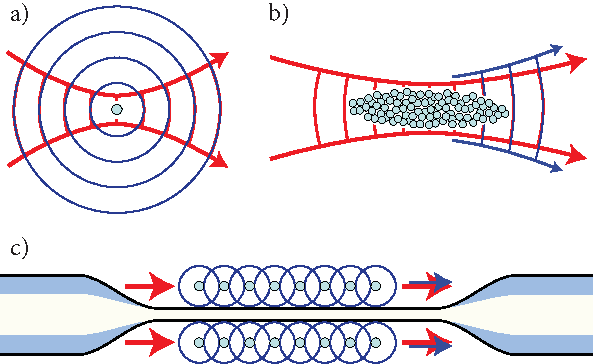
\includegraphics[scale=1.10]{../chap4/Fig1}
\caption[Comparing mode-matching and cooperativity of quantum interfaces in free-space and a nanofiber.]{Cooperativity and mode-matching for various atom-light geometries. (a) The  beam area at the waist of a tightly focused beam is closely matched with the atomic scattering cross section, but the scattered light of a single atom is poorly mode-matched with the probe. (b) A paraxial beam probing a rarefied atomic cloud whose scattered radiation interferes constructively in the forward direction. (c) Atoms trapped in a 1D optical lattices  near the surface of an optical nanofiber interacting with a fiber-guided probe. The tight confinement and automatic mode matching that accompanies scattering into the guided mode leads to strong cooperativity in the atom-photon interaction.}\label{Fig::ModeMatching}
\end{figure}
%=============================================

A particular system that combines the elements above consists of cold atoms trapped in the evanescent field of the guided mode of a tapered optical nanofiber with a subwavelength diameter \cite{vetsch_optical_2010, lacroute_state-insensitive_2012, balykin_quantum_2014, grover_photon-correlation_2015, Lee2015Inhomogeneous} (see \frf{Fig::ModeMatching}).  
The typical resonant OD per atom, or OD/$N_A$, in the nanofiber ($\sigma_0/A \sim  10^{-2}$) is boosted by orders of magnitude over free space for paraxial beams. 
However, one cannot reach the strong coupling regime where $\Gamma_{\oneD}$ is on the order of $\Gamma_{\vac}$ as is possible in engineered nanophotonic waveguides, such as those arising in photonic crystals \cite{hung_trapped_2013}, where atoms can be trapped at positions of peak intensity of the field.  
One can, however, achieve strong cooperativity in the dispersive regime with a moderately sized ensemble.  When compared to free space, all light scattered into the guided mode is automatically mode matched, and thus, given the relatively large ratio $\sigma_0/A$, one can achieve high OD with only a few thousand atoms (see \frf{Fig::ModeMatching}).  
Such strong cooperativity opens the door to new regimes to create non-Gaussian quantum states of the ensemble \cite{dubost_efficient_2012} and potentially to implement nonlinear optics at the level of a few photons \cite{spillane_observation_2008, pittman_ultralow-power_2013, oshea_fiber-optical_2013}.


One-dimensional optical lattices in nanofibers based on multiple co- and counter-propagating trapping beams have been loaded with up to several thousand alkali atoms \cite{vetsch_optical_2010, lacroute_state-insensitive_2012}.
This has proved a fruitful platform for quantum information processing.  
The anisotropic nature of the strong atom-light coupling has been exploited for control of internal atomic states \cite{mitsch_exploiting_2014}, enhanced coupling into a preferred propagation direction \cite{petersen_chiral_2014, mitsch_quantum_2014}, and optical switching \cite{oshea_fiber-optical_2013}. 
Off resonance, dispersive coupling has allowed for non-destructive atom counting \cite{dawkins_dispersive_2011, beguin_generation_2014} 
and storage of fiber-guided light \cite{gouraud_demonstration_2015, sayrin_storage_2015}.
Recent demonstrations of photonic crystal cavities fabricated on the nanofiber \cite{wuttke_nanofiber_2012, nayak_optical_2014, schell_highly_2015} promise further enhanced atom-light coupling.

In this chapter we study the quantum atom-light interface in the dispersive regime for an optical nanofiber geometry.  We focus here on the coupling between the atomic spin and light polarization induced by the elastic scattering of photons by tensor-polarizable cesium atoms trapped near the surface of the nanofiber.  This provides an entangling interaction that can be employed to generate spin squeezing via QND measurement.  Our analysis unifies a variety of different approaches found in the literature, including direct calculation of the dyadic Green's function for photon scattering \cite{Sakoda1996Optical, Dung2000, Sondergaard2001, Klimov2004, Wubs2004, Fussell2005Decay, MangaRao2007Single, dzsotjan_quantum_2010} and the input-output formalism studied for one-dimensional field theories based on Heisenberg-Langevin equations \cite{Gardiner1985Input, Blow1990Continuum, shen_coherent_2005, LeKien2005a, LeKien2008, fan_input-output_2010}.

The remainder of this article is organized as follows.  
In \srf{Sec::GreensFunction} we solve for the mode decomposition of the dyadic Green's function which determines the electric field scattered by a point dipole near the surface of the nanofiber.  
This allows us to calculate the phase shift and polarization transformation for fiber-guided photons induced by tensor-polarizable atoms in the dispersive regime.  
We connect this with a fully quantum mechanical treatment based on a Heisenberg-Langevin picture in \srf{Sec::HeisenbergLangevin}.  
The formalism we develop is used in \srf{Sec::QNDMeasurement} to study QND measurement of atoms based on polarization spectroscopy. 
We consider shot-noise-limited atom detection as well as measurement-backaction-induced squeezing of spin projection noise.  
We study squeezing of the collective pseudospin associated with ensembles of atoms in the atomic clock state and calculate its dynamics based on a first principles stochastic master equation that includes both the effects of QND measurement as well as decoherence due to optical pumping.  
We conclude with a summary and outlook for future research in \srf{Sec::Conclusion}.  


%========GREEN'S FUNCTION AND INPUT/OUTPUT RESPONSE=========%
\section{Dyadic Green's function and input-output\\ field response} \label{Sec::GreensFunction}

Given a point particle with tensor polarizability $\tensor{\boldsymbol{\alpha}}$ at position $\br'$ near the surface of a nanofiber, the field  at frequency $\omega_0$ is given by the solution to the wave equation, 
	\begin{align}\label{Eq::WaveEquationSource}
		\left[ - \nabla\times\nabla\times + \, n^2(\br)k_0^2 \right] \mathbf{E}(\br) &= -4\pi  k_0^2 \delta^{(3)}(\br-\br')\,  \tensor{\boldsymbol{\alpha}}\cdot \mathbf{E}(\br),
	\end{align}
where $k_0=\omega_0/c$ and $n(\mbf{r})$ is the spatially varying index of refraction that describes the fiber; Gaussian-cgs units are used throughout.  
For an asymptotic input field $\mathbf{E}_{\inp}(\br)$, the scattering solution to \erf{Eq::WaveEquationSource} is given by the Lippmann-Schwinger equation \cite{Wubs2004},
\begin{subequations}
	\begin{align}
		\mathbf{E}_{\out}(\br) &=\mathbf{E}_{\inp}(\br)+\tensor{\mathbf{G}}^{(+)}(\br , \br'; \omega_0)\cdot 
\tensor{\boldsymbol{\alpha}}\cdot \mathbf{E}_{\out}(\br')\\
		&\approx \mathbf{E}_{\inp}(\br)+ \tensor{\mathbf{G}}^{(+)}(\br , \br'; \omega_0) \cdot 
\tensor{\boldsymbol{\alpha}}\cdot \mathbf{E}_{\inp}(\br'), \label{Eq::ScatteredField}
	\end{align}
\end{subequations}
where in \erf{Eq::ScatteredField} we have made the first Born approximation valid for weak scattering. The fundamental object that fully characterizes the scattered radiation as well as the energy level shift and modified decay rate of a scatterer near the dielectric is the dyadic Green's function, $\tensor{\mathbf{G}}(\br, \br';\omega_0)$. This determines the scattered field from a point dipole at $\br'$, $\mathbf{E}_{\rm scat}(\br)= \tensor{\mathbf{G}}^{(+)}(\br , \br'; \omega_0)\cdot \mathbf{d}$, and satisfies the equation of motion,
	\begin{align} \label{Eq::GreensDiffEq}
		\left[ -\nabla\times\nabla\times + n^2(\mbf{r}) k_0^2 \right] \tensor{\mathbf{G}}(\br, \br';\omega_0) &= -4\pi 
k_0^2 \delta^{(3)}(\mathbf{r}-\mathbf{r}') \unittens,
	\end{align}
where $\unittens$ is the unit tensor.   

The solution for the Green's function $\tensor{\mathbf{G}}(\br ,\br' ; \omega_0)$, following from Maxwell's equations,  
has been studied previously \cite{Sakoda1996Optical,Sondergaard2001,Wubs2004}.
In Chapter 2, we have also derived the eigenmode decomposition solutions for the dyadic Green's function of a nanophotonic waveguide and shown that the radiation modes do not contribute to the sign measured at the end of the waveguide. 
As we are interested here in the forward-scattered components that lead to phase shifts and polarization transformations, we apply the eigenmode decomposition approach derived in Chapter 2 to directly calculate a nanofiber's $\tensor{\mathbf{G}}(\br ,\br' ; \omega_0)$ using the fiber's normal modes and study how the guided modes respond to atoms with a tensor polarizability. 

We treat an optical nanofiber of radius $a$ with step-index profile,
	\begin{align} \label{Eq::IndexofRefraction}
		n(r_\perp) = \Big\{  
			\begin{array}{l l} n_1 & \quad r \leq a \\
						 n_2 & \quad r > a 
		\end{array},
	\end{align}
for a silica core ($n_1 = 1.4469$)~\cite{Kien2004} and infinite vacuum cladding ($n_2 = 1$).  For a cylindrically symmetric dielectric the guided modes are $\mathbf{f}_\mu (\br) = \mathbf{u}_\mu (\br_\perp) e^{i\beta z}/\sqrt{2 \pi}$, with indices $\mu=\{j, \beta , p\}$ for the $j$th guided mode with propagation constant $\beta$ at frequency $\omega_\mu=\omega(\beta)$ and polarization $p$. 
Two convenient guided-mode bases to describe $ \mathbf{u}_\mu (\br_\perp) $ are the quasilinear and quasicircular polarization modes, described in Appendix \ref{chap:fibereigenmodes} \cite{Kien2004}.  

We consider nanofibers that support only the lowest HE$_{11}$ guided modes at the relevant frequency $\omega_0$ \cite{Snyder1983Optical}, which have four guided modes: two polarizations $p$, each with propagation constant $\beta(\omega_0) = \pm\beta_0$ corresponding to forward and backward propagation. We use $ b=\pm $ to indicate the propagation direction. Substituting the guided mode indices into Eq.~\eqref{Eq::GreensGuided_general}, the guided-mode contribution to the dyadic Greens function for $ z\neq z' $ is then 
	\begin{align} 
		\tensor{\mathbf{G}}^{(+)}_g(\br,\br'; \omega_0) = &2\pi i \sum_{b,p}  {\rm Res}\vert_{\beta =b\beta_0} 
\left[\frac{-2 \omega_0^2 }{ \omega_0^2-\omega^2(\beta)}\right]  \mathbf{u}_{b\beta_0, p} 
(\br_\perp)\mathbf{u}^*_{b\beta_0, p} (\br_{\perp}^\prime)e^{ib \beta_0 (z-z')} \nonumber \\
= & 2\pi i \frac{\omega_0}{v_g } \sum_{b,p} \mathbf{u}_{b, p} (\br_\perp)\mathbf{u}^*_{b, p} 
(\br_{\perp}^\prime) e^{i b\beta_0(z-z')} \Theta \big( b(z-z') \big), \label{Eq::GreensGuided}
	\end{align}
where $v_g= \vert d\omega/d\beta \vert_{\beta=\beta_0}$ is the group velocity of the HE$_{11}$ modes at $\omega_0$, and $\Theta \big( b(z-z') \big)$ is a Heaviside function. At $ \br=\br' $, Eq.~\eqref{Eq::ImGreenLocal_general} yields the imaginary part of the dyadic Green's function:
	\begin{equation}\label{Eq::ImGreenLocal}
		{\rm Im} \big[\tensor{\mathbf{G}}^{(+)}_g(\br',\br'; \omega_0=\omega_{eg}) \big] = \pi \frac{\omega_{eg}}{v_g } \sum_{b, p} 
		\mathbf{u}_{b, p} (\br_{\!\perp}^\prime)\mathbf{u}^*_{b , p} (\br_{\!\perp}^\prime),
	\end{equation}
where we have used $\omega_0=\omega_{eg}$ for future calculations of the decay rates of the quantum transitions between the ground state $ \ket{g} $ and the excited state $ \ket{e} $ of the atom.  The real part of the Green's function at $\br = \br'$ determines the energy level shift of the scatterer. 

Equation (\ref{Eq::GreensGuided}) is the central result from which we can calculate the dispersive response.  Consider a forward-propagating input field in the guided modes with frequency $\omega_0$, positive-frequency amplitude $\Eamp$, and arbitrary polarization, $\mathbf{E}^{(+)}_{\inp}(\br) = \Eamp  \mathbf{u}_{\rm in}(\br_\perp) e^{i \beta_0 z}$ dispersively coupled to an atom at position $\mathbf{r}'$.  The effective mode area at the atom's position is determined from the total cycle-averaged power transported along the nanofiber, $P_{{\rm in},z} = (v_g/2\pi) \int d^2\br \, n^2(r_\perp) |\mathbf{E}^{(+)}_{\inp}(\br) |^2$, and the intensity at the atom, $I_{\rm in}(\mathbf{r}') = (c/2\pi) |\mathbf{E}^{(+)}_{\inp}(\br') |^2$, via the relation \cite{domokos_quantum_2002},
 	\begin{align} \label{Eq::AreaIn}
 		A_{\rm in} \equiv \frac{P_{{\rm in}}}{I_{\rm in}(\mathbf{r}')} = \frac{1}{n_g |\mathbf{u}_{\rm in}(\mathbf{r}'_\perp)|^{2}},
	\end{align}
where $n_g\equiv c/v_g$ is the group index of refraction.    

Substitution of the guided-mode Green's function, \erf{Eq::GreensGuided}, into the Lippman-Schwinger equation, \erf{Eq::ScatteredField}, yields the transmitted (forward-scattered) and reflected (backward-scattered) output fields, \begin{equation}
\mathbf{E}_{\out}(\br) = \Eamp \big[ \mathbf{u}_{\trans, \out} (\br_\perp) e^{i \beta_0 z} + \mathbf{u}_{\refl,\out} (\br_\perp) e^{-i \beta_0 z} \big],
\end{equation}
where 
\begin{subequations}
	\begin{align}
		\mathbf{u}_{\trans, \out} (\br_\perp) &=  \sum_{p,p'}  \, c_{p} t_{pp'} \mathbf{u}_{\fwd, p'}(\br_\perp) \\ 
		\mathbf{u}_{\refl,\out} (\br_\perp) &=  \sum_{p,p'}  \, c_{p} r_{pp'} \mathbf{u}_{\bwd, p'}(\br_\perp),
	\end{align}
\end{subequations}
where we have decomposed the input into the polarization eigenmodes, $\mbf{u}_{\rm in}(\mbf{r}_\perp) = \sum_{p} c_{p} \mathbf{u}_{\fwd,p}(\br_\perp)$.  
For $z>z'$, the transmission and reflection matrices are 
\begin{subequations}
	\begin{align} \label{Eq::PolarizationTransformation}
		t_{pp'} =& \delta_{p,p'} +  2\pi i k_0 n_g \, \mathbf{u}^*_{+, p}(\br'_\perp) \cdot 
\tensor{\boldsymbol{\alpha}} \cdot \mathbf{u}_{+, p'}(\br'_\perp) , \\
		r_{pp'} =&  2\pi i k_0 n_g \, \mathbf{u}^*_{\bwd, p}(\br'_\perp) \cdot 
\tensor{\boldsymbol{\alpha}} \cdot \mathbf{u}_{\fwd, p'}(\br'_\perp) e^{2 i\beta_0 z'} , 
	\end{align} 
\end{subequations}
We focus here on the transmitted fields whose interference with the input field for $z>z'$ results in a phase shift and a polarization transformation.  
For weak scattering the diagonal terms, $t_{p p} \approx \sqrt{1-R_p}e^{i \delta \phi_p}$, determine the phase shift and attenuation induced on each polarization mode,
\begin{subequations}
	\begin{align}
		 \delta \phi_p &= \frac{2 \pi k_0}{A_{\rm in}} {\rm Re}(\alpha_{pp}),  \label{Eq::PhaseShift} \\
		R_p &=  \frac{4 \pi k_0}{A_{\rm in}} {\rm Im}(\alpha_{pp}) .\label{Eq::Attenuation} 
	\end{align} 
\end{subequations}
Here, the $\{p,p'\}$-element of the tensor polarizability is given by, $\alpha_{pp'} \equiv \mathbf{e}^*_{p'} \cdot \tensor{\boldsymbol{\alpha}}\cdot \mathbf{e}_{p}$, with unit vectors for each of the forward-propagating mode functions,\linebreak[4] $\mathbf{e}_{p}\equiv \mathbf{u}_{+,p}(\br'_\perp)/|\mathbf{u}_{+,p}(\br'_\perp)|$. 

The phase shift per atom, \erf{Eq::PhaseShift}, is modified over free space in two ways, both of which are captured by the effective mode area $A_{\rm in}$. First, although material dispersion in an optical fiber is negligible over the distances we consider, additional waveguide dispersion can lead to a significant reduction in the group velocity~\cite{hung_trapped_2013,goban_atomlight_2014}.  Such ``slow light" enhances the atom-photon coupling strength. 
In the nanofiber geometry this effect is moderate -- we calculated the group index to be $n_g \approx 1.40$. 
Second and more importantly, the tight spatial confinement as measured by OD/$N_A$ significantly increases the coupling strength over free space for every atom along the nanofiber, which yields strong cooperativity.
In contrast, in free space diffraction restricts the collective phase shift for an ensemble of atoms~\cite{tanji-suzuki_chapter_2011, baragiola_three-dimensional_2014}.  
For a Gaussian beam with beam waist $w_0$, the total phase shift induced by a collection of polarizable atoms will be $\delta \phi = N_{\eff} 2 \pi k_0 {\rm Re}({\alpha})/A$, where $A = \pi w^2_0/2$ is the beam area at the focus and $N_{\eff}$ is the effective number of atoms that radiate into this mode.  
One can couple strongly to few atoms at the center by tightly focusing the beam or couple weakly to many atoms by choosing a larger focal volume, but hence, smaller cooperativity per atom.  

The off-diagonal terms in the transmission matrix, \erf{Eq::PolarizationTransformation}, describe the polarization transformation. For example, if we take the polarization of the modes to be the quasilinear, $p = \{H,V\}$ as defined in \erf{Eq::QuasilinearModes}, then $t_{HV} \equiv \chi_{\rm Far}$ is the rotation angle of the Stokes vector on the Poincar\'{e} sphere corresponding to the Faraday effect \cite{hammerer_quantum_2010, Deutsch2010a}.  
The phase difference in that basis, $\delta  \phi_H - \delta \phi_V$, corresponds to birefringence induced on the guided mode and $t_{HV}$ to Faraday rotation.  
Analyzed in the quasicircular polarization modes ($p=\pm$), given in \erf{Eq::QuasicircularModes}, the differential phase $\delta \phi_+ -\delta  \phi_-$ corresponds to Faraday rotation and $t_{+-}$ to birefringence.  
We make use of such polarization transformations as a means to nondestructively measure the atoms and generate collective spin squeezing.

	
%===================Heisenberg-Langevin Equations=====================%
\section{Heisenberg-Langevin-picture solution\\ and atomic response} \label{Sec::HeisenbergLangevin}
	
The Lippmann-Schwinger solution, \erf{Eq::ScatteredField}, determines the input-output relation for linear atomic response given by the polarizability tensor $\tensor{\alpha}$.  
In this section we connect this with the fully quantum mechanical description of dispersive atomic response and input-output relations for the quantized guided modes.  
Following Ref. \cite{LeKien2005a}, we use a Heisenberg-Langevin approach for one-dimensional systems.  

The positive frequency component of the quantized electric field operator decomposes into guided and radiation (unguided) modes, $\hat{\mathbf{E}}^{(+)}=\hat{\mathbf{E}}_g^{(+)}+\hat{\mathbf{E}}_{r}^{(+)}$, where
\begin{subequations}
	\begin{align}
		\hat{\mathbf{E}}_g^{(+)}(\br) &= \sum_{b,p} \int_0^{\infty}\!\!\!\!\!  \mathrm{d}\omega \sqrt{\frac{ \hbar \omega}{ v_g}} \; \awg \mathbf{u}_\mu (\br\!_\perp) e^{i b\beta(\omega) z } ,\label{Eq::QuantizedElectricField} \\
		\hat{\mathbf{E}}_r^{(+)}(\br) &= \sum_{m,p}\int_0^{\infty}\!\!\!\!\! \mathrm{d}\omega   \int_{-kn_2}^{kn_2}\mathrm{d}\beta \, \sqrt{ \hbar \omega}\;\awr \mathbf{u}_\nu (\br\!_\perp) e^{i\beta(\omega) z }.
	\end{align}
\end{subequations}
The HE$_{11}$ guided modes are specified by $\mu =(\omega, b, p)$, where $\omega$ is the mode frequency,  $p$ is the polarization, and the propagation direction $b=\pm$ corresponds to wavenumber $b \beta (\omega)$.  The radiation modes are specified by  $\nu=(\omega, \beta, m, p)$, where $m$ is the azimuthal (angular momentum) quantum number, $p$ labels the two orthogonal polarizations, and longitudinal propagation constant $\beta$ can vary continuously from $-kn_2$ to $kn_2$, with $k = \omega/c$ \cite{Sondergaard2001,LeKien2005a}.  
The creation/annihilation operators satisfy the usual continuous-mode commutation relations, $[\hat{a}_\mu, \hat{a}^\dag_{\mu'} ] = \delta_{b,b'} \delta_{p,p'} \delta ( \omega - \omega ') $ and $[\hat{a}_\nu ,\hat{a}^\dag_{\nu'} ] = \delta_{m,m'} \delta_{p,p'} \delta ( \omega - \omega ')  \delta ( \beta - \beta') $.

The Hamiltonian for the system is
\begin{equation}
\hat{H} = \hat{H}_F+\hat{H}_A + \hat{H}_{\inter},
\end{equation}
where the free-field Hamiltonian decomposes into guided and unguided modes, 
	\begin{equation}
		\hat{H}_F = \sum_{b,p}\int_0^{\infty}\!\!\!\!\! \mathrm{d}\omega \, \hbar \omega \hat{a}^\dagger_\mu \hat{a}_\mu 
+\sum_{m,p} \int_0^{\infty}\!\!\!\!\! \mathrm{d}\omega  \int_{-k n_2}^{k n_2} \mathrm{d}\beta \, \hbar \omega 
\hat{a}^\dagger_\nu \hat{a}_\nu.
	\end{equation}
We consider here alkali atoms with ground and excited levels, $\{ \ket{g}=\ket{nS_{1/2}, f, m_f}\}$, $\{ \ket{e} =\ket{nP_{j'}, f', m_{f'}}\}$, where $\ket{f, m_f}$ denotes the hyperfine sublevels.  The free atomic Hamiltonian is
	\begin{equation}
		\hat{H}_A  = \sum_g E_g \hat{\sigma}_{gg} + \sum_e E_e \hat{\sigma}_{ee},
	\end{equation}
where $\hat{\sigma}_{ij} \equiv \ket{i}\bra{j}$.  In the rotating wave approximation, the atom-field interaction Hamiltonian is
	\begin{align}
		\hat{H}_{\inter} &= -\hat{\mathbf{d}}\cdot \hat{\mathbf{E}} =- \sum_{e,g} \left[ \hat{\mathbf{d}}_{eg}\cdot 
\hat{\mathbf{E}}^{(+)}(\br')+\hat{\mathbf{d}}_{ge}\cdot \hat{\mathbf{E}}^{(-)}(\br') \right],
	\end{align}
where the atomic dipole operator is projected between excited and ground subspaces, $\hat{\mathbf{d}}_{eg}= \hat{P}_e \hat{\mathbf{d}} \hat{P}_g $. The interaction Hamiltonian then takes the form, 
\begin{equation}
	\hat{H}_{\inter} = -\sum_{e,g} \left(\sum_{b,p} \int_0^{\infty}\!\!\!\!\!\mathrm{d}\omega \; \hbar g_{\mu, e,g}\, \hat{a}_\mu  \, 
		\hat{\sigma}_{eg}+ \sum_{m,p} \int_0^{\infty}\!\!\!\!\!\mathrm{d}\omega \! \int_{-kn_2}^{kn_2}\mathrm{d}\beta \,  \hbar 
g_{\nu, e,g}\, \hat{a}_\nu \, \hat{\sigma}_{eg}\right) + {H.c.},
	\end{equation}
where the coupling constants for guided/radiation modes are
\begin{subequations} \label{Eq::CouplingConstants}
	\begin{align}
		\hbar g_{\mu, e,g} &= \sqrt{\frac{\hbar \omega}{ v_g  }}\, \bra{e} \hat{\mathbf{d}} \ket{g} 
\cdot\mathbf{u}_\mu ( \br'_\perp ) e^{i b \beta(\omega)z} , \\
		\hbar g_{\nu, e,g} &= \sqrt{  \hbar \omega } \, \bra{e} \hat{\mathbf{d}} \ket{g} \cdot \mathbf{u}_\nu ( \br'_\perp) e^{i\beta(\omega)z}  .
	\end{align}
\end{subequations}
The Heisenberg equations of motion are
\begin{subequations}
	\begin{align}
		\der{\hat{a}_\mu} &= -i\omega \hat{a}_\mu +i\sum_{e,g} g_{\mu, e,g}^* \hat{\sigma}_{ge} \label{eq:da},\\
		\der{\hat{a}_\nu} &= -i\omega \hat{a}_\nu +i\sum_{e,g} g_{\nu, e,g}^*  \hat{\sigma}_{ge}\label{eq:danu},\\
		\der{\hat{\sigma}_{ge}} &= -i\omega_{eg} \hat{\sigma}_{ge} \label{Eq::dsigma}  \\
			&+ i\!\int_0^{\infty}\!\!\!\!\! \mathrm{d}\omega \sum_{e',g'} \bigg\{ \big(\delta_{ee'} \hat{\sigma}_{gg'} \!-\! \delta_{gg'} \hat{\sigma}_{e'e} \big) \bigg[ \sum_{b,p}  g_{\mu, e',g'}\hat{a}_\mu \!+\! \sum_{m,p} \!\int_{-kn_2}^{kn_2}\!\!\!\!\!\! \mathrm{d}\beta \; g_{\nu, e',g'} \hat{a}_\nu \bigg] \bigg\}. \nonumber
	\end{align}
\end{subequations}
Integrating the field equations, 
\begin{subequations}\label{eq:aout1}
\begin{align}
\hat{a}_\mu(t) &= \hat{a}_\mu(t_0) e^{-i\omega (t-t_0)} +i \sum_{e,g} g_{\mu,e,g}^* \int_{t_0}^t 
\mathrm{d} t' e^{-i\omega (t-t')}\hat{\sigma}_{ge}(t'), \label{Eq::aguidedEOM}
\end{align}
\begin{align}
\hat{a}_\nu (t) &= \hat{a}_\nu (t_0) e^{-i\omega (t-t_0)} +i \sum_{e,g} g_{\nu,e,g}^* \int_{t_0}^t \mathrm{d} 
t' e^{-i\omega (t-t')}\hat{\sigma}_{ge}(t'),
\end{align}
\end{subequations}
substituting into \erf{Eq::dsigma}, and making the usual Markov\linebreak[4] approximation \cite{LeKien2005a} gives an expression for the ground-excited coherences.   This yields
\begin{align}
&\quad\dt{\hat{\sigma}_{ge}} =-i\omega_{eg} 
\hat{\sigma}_{ge}-\sum_{e'}\frac{\Gamma_{ee'}}{2}\hat{\sigma}_{ge'}  \\
&\!+i\! \sum_{e',g'}\!\!\bigg\{\!\! (\delta_{e,e'} \hat{\sigma}_{\!gg'} \!-\! \delta_{g,g'} 
\hat{\sigma}_{e'e})\!\!\int_0^{\infty}\!\!\!\!\!\!\mathrm{d}\omega \!\bigg[\! \sum_{b,p}  \!g_{\mu, e'\!,g'} \hat{a}_\mu (t_0) 
\!+\!\! \sum_{m,p}\!\!  \int_{-kn_2}^{kn_2}\!\!\!\!\!\!\!\!\!\mathrm{d}\beta  g_{\nu, e'\!,g'} \hat{a}_\nu(t_0) \!\bigg]\! e^{-i\omega 
(t-t_0)}\!\bigg\}\!, \nonumber
\end{align}
where the decay rates of excited-populations and coherences are given by 
	\begin{equation}
		\Gamma_{ee'} = 2\pi \sum_{\mu,g} g_{\mu,e,g}g^*_{\mu,e',g} \vert_{\omega=\omega_{eg}}+2\pi 
\sum_{m,p,g} \int_{-kn_2}^{kn_2}\!\!\!\!\! d\beta \, g_{\nu,e,g}g^*_{\nu,e',g} \vert_{\omega=\omega_{eg}}, \label{Eq::TotaleeDecayRate}
	\end{equation}
and the small energy shift is absorbed into the transition frequency $\omega_{eg} = (E_e - E_g)/\hbar$.  
Equation (\ref{Eq::TotaleeDecayRate}) captures the modification of the spontaneous emission rate due to the nanofiber.  
The first sum describes decay into the guided modes and the second into the unguided radiation modes \cite{ nha_cavity_1997,Klimov2004,LeKien2005a,maslov_distribution_2006, scheel_directional_2015}. The decay rate of a given excited state into all guided modes is given by
	\begin{equation}
		\Gamma_e^{\oneD}= 2\pi \sum_{b,p,g} |g_{\mu,e,g} |^2_{\omega = \omega_{eg}} =  \frac{ 2\pi }{\hbar} \frac{ \omega_{eg} }{v_g} \sum_{b,p,g} \big|\bra{e}\hat{\mathbf{d}}\ket{g} \cdot \mathbf{u}_{bp}(\br'_\perp)\big|^2  .
	\end{equation}
This is in agreement with the expected expression from the guided-mode contribution to the dyadic Green's function in \erf{Eq::ImGreenLocal},
	\begin{equation} \label{Eq::Gamma1DGreens}
		\Gamma_e^{\oneD} =  \frac{2}{\hbar} \sum_{g}  \bra{g}\hat{\mathbf{d}}\ket{e}\cdot 
{\rm Im} \Big[\tensor{\mathbf{G}}^{(+)}_g(\br', \br'; \omega_{eg} ) \Big] \cdot \bra{e}\hat{\mathbf{d}}\ket{g},
	\end{equation}
which is enhanced over the free-space rate by the Purcell factor. 

Here we are interested in linear response for excitation far from resonance. We follow Ref. \cite{le_kien_propagation_2014} and consider an atom sufficiently far from the fiber surface such that the modification of the spontaneous emission rate is small.   In this case the decay rate is approximated as $\Gamma_{ee'} \approx \delta_{e,e'} \Gamma_{e}$, where $\Gamma_e$ is the total decay rate from excited state $\ket{e}$, given by the diagonal elements of \erf{Eq::TotaleeDecayRate}.  In steady state, the dipole operator in the linear regime ($\hat{\sigma}_{ee'} \rightarrow 0 $) is approximately
	\begin{align}
		\hat{\sigma}_{ge} \approx -\sum_{g'} \hat{\sigma}_{gg'}\int_0^{\infty}\mathrm{d}\omega \bigg( & \sum_{b,p}  
\frac{g_{\mu, e,g'}}{\omega-\omega_{eg} + i \Gamma_{e}/2  }\, \hat{a}_\mu (t_0) \\
	&+\sum_{m,p} \int_{-kn_2}^{kn_2}\mathrm{d}\beta \, \frac{g_{\nu, e,g'}}{\omega-\omega_{eg} + i \Gamma_{e}/2 } \,\hat{a}_\nu (t_0)  \bigg)e^{-i\omega (t-t_0)} . \nn
	\end{align}
By substituting this into \erf{Eq::aguidedEOM} and defining asymptotic modes, $\hat{a}^{\inp}(\omega) = \lim_{t_0\rightarrow -\infty} \hat{a}(t_0) e^{i\omega t_0}$, $\hat{a}^{\out}(\omega) = \lim_{t\rightarrow +\infty} \hat{a}(t) e^{i\omega t}$ \cite{fan_input-output_2010}, we obtain the input-output relationship for the guided modes, 
	\begin{align} \label{Eq::aout}
		\hat{a}^{\out}_\mu (\omega) \!= \hat{a}^{\inp}_\mu (\omega) &-\! 2\pi i\sum_{b',p'} 
\sum_{e,g,g'}\!\!\hat{\sigma}_{gg'}\frac{ g_{\mu,e,g}^* g_{\mu'\!\!,e,g'}}{ \omega \!-\! \omega_{eg} \!+\! i \Gamma\!_{e}/2 }\hat{a}^{\inp}_{\mu'}(\omega) \nn\\
&-\! 2\pi i\!\sum_{m\!,p} \sum_{e\!,g\!,g'}\! \int^{kn_2}_{-kn_2}\!\!\!\! \mathrm{d}\beta \,\hat{\sigma}\!_{gg'}\frac{ g_{\mu,e,g}^* g_{\nu'\!\!,e,g'}}{ \omega \!-\! \omega_{eg} \!\!+\! i \Gamma\!_{e}/2 }\hat{a}^{\inp}_{\nu}(\omega).
	\end{align}
	
This input-output relation contains the phase shift on forward scattered modes as well as attenuation due to elastic scattering into all other modes. For a probe with frequency $\omega_0$, \erf{Eq::aout} agrees with the expected form given by the Lippmann-Schwinger equation in the first Born approximation \footnote{In a careful derivation of the Lippman-Schwinger scattering equation, it is not the total Green's function that appears in \erf{Eq::ScatteredField} but rather a related dyadic quantity, $\mbf{K}(\br,\br', \omega_0) = \mbf{G}(\br,\br', \omega_0) + \delta(\br-\br')/n^2(\br)$ \cite{Wubs2004}. 
This function arises by proper accounting of the scatterer's coupling to the \emph{displacement} rather than the electric field \cite{yao_ultrahigh_2009} with a distinction that becomes important at the source point $\mbf{r} = \mbf{r}'$. However, for lossless dielectrics $n(\mathbf{r})$ is real and ${\rm Im}[\tensor{\mathbf{G}}(\br',\br'; \omega)] = {\rm Im}[\tensor{\mathbf{K}}(\br',\br'; \omega)]$ \cite{yao_-chip_2010}. },
	\begin{equation} \label{Eq::IOScatteredField}
		\hat{\mathbf{E}}^{(+)}_{\out,g}(\br, \omega_0)=\hat{\mathbf{E}}^{(+)}_{ \inp, g}(\br, \omega_0)+\tensor{\mathbf{G}}_g^{(+)}(\br,\br', \omega_0)\cdot \poltens \cdot \big[\hat{\mathbf{E}}^{(+)}_{\inp, g}(\br', \omega_0)+\hat{\mathbf{E}}^{(+)}_{\inp,r}(\br', \omega_0) \big],
	\end{equation}
by noting that for the guided-mode dyadic Green's function given in \erf{Eq::GreensGuided},
	\begin{align}
		\int d^2 \mbf{r}_\perp \, \mathbf{u}^*_{\mu} (\br_\perp)\cdot \tensor{\mathbf{G}}_g^{(+)}(\br,\br',\omega_0)\cdot \poltens \cdot \mathbf{u}_{\mu'} (\br'_\perp) &= i \frac{ 2\pi \omega_0}{v_g} \mathbf{u}^*_{b,p} (\br'_\perp) \cdot \poltens \cdot \mathbf{u}_{b'\!\!, p'} (\br'_\perp).  
	\end{align}
Here, the atomic polarizability operator \cite{buhmann_casimir-polder_2004, Deutsch2010a,LeKien2013}, is given by
	\begin{equation} \label{Eq::PolarizabilityOperator}
		\poltens = - \frac{1}{\hbar} \sum_{e,g,g'}\ket{g}\frac{\bra{g}\hat{\mathbf{d}}\ket{e}\bra{e} 
\hat{\mathbf{d}}\ket{g'}}{\Delta_{eg} + i \Gamma_{e}/2 }\bra{g'},
	\end{equation}	
and $\Delta_{eg} = \omega_0 - \omega_{eg}$ is the laser detuning from the atomic transition.	
For an atom in ground state $\ket{g}$ and polarization $p$, the phase shift can be expressed as \cite{le_kien_propagation_2014}
	\begin{align} \label{Eq::PhaseShiftMultilevel}
		\delta  \phi_{p,g} &=2\pi \frac{ \omega_{0} }{v_g} \mathbf{u}^*_{+, p}(\br'_\perp) \cdot {\rm Re}\big[\bra{g} \hat{\tensor{\boldsymbol{\alpha}}} \ket{g} \big] \cdot \mathbf{u}_{+, p}(\br'_\perp)\nonumber\\
		&= -\frac{ \omega_{0} }{v_g} \sum_e \frac{2 \pi |\bra{e}\hat{\mathbf{d}}\ket{g} \cdot \mathbf{u}_{+,p}(\br'_\perp)|^2}{ \hbar  \Delta_{eg} } .
	\end{align}  
We employ this dispersive response for QND measurement of atoms, as we describe in the next section.



%============== SECITON: QND Measurement ==============%
\section{QND measurement of atoms} \label{Sec::QNDMeasurement}

%========= FIGURE: Geometry (coupling strength, magic wavelength, area and detuning) =========%
\begin{figure}[t]
\centering
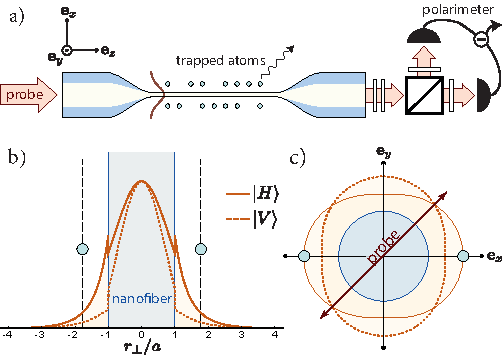
\includegraphics[scale=1.5]{../chap4/Fig2}
\caption[Quantum interface for spin-polarization coupling of two 1D lattices of cold, trapped atoms and the guided modes of an optical nanofiber based on the birefringence effect.]{Quantum interface for spin-polarization coupling of two 1D lattices of cold, trapped atoms and the guided modes of an optical nanofiber. a) Schematic of the interface.  A linearly polarized probe is launched into the nanofiber and the output light is analyzed in a polarimeter.  The atoms (green circles), trapped in the $x$-$z$ plane, couple to the evanescent portion of the guided $H$ and $V$ modes.  Contours of the $H$- and $V$-mode intensities in b) the $x$direction and c) the transverse $xy$ plane show the mode anisotropy at the atomic positions. }\label{Fig::Schematic}
\end{figure}
%=============================================

The dispersive interface between the atoms and nanofiber guided photons provides the entangling mechanism necessary to perform a QND measurement on the atoms.  
We restrict here to the quasilinear modes, $p =\{H,V\}$, of a single HE$_{11}$ guided mode at frequency $\omega_0$, whose form is given explicitly in \erf{Eq::QuasilinearModes}.  
In typical experimental configurations, two one-dimensional arrays of atoms are trapped on either side of the nanofiber, see Fig. \ref{Fig::Schematic}. 
We define coordinate axes $(x,y,z)$ with $z$ oriented along the fiber axis for forward propagation, and the two chains of atoms lie in the $x$-$z$ plane at azimuthal angles $\phi' = \{0, \pi\}$.
In the evanescent region, the $H$ mode is purely $\mathbf{e}_x$-polarized at $\phi = \pm \pi/2$ and the $V$ mode is purely $\mathbf{e}_y$-polarized at $\phi = \{0,\pi\}$.  
At other azimuthal angles the electric field is generally rotating along an ellipse in the $x$-$z$ plane.  The atoms at $\phi'=0$ experience $H$ and $V$ fields,
\begin{subequations}
	\begin{align}
		\mbf{u}_{b,H}(r_\perp, \phi = 0) = & \sqrt{2} \big[ \mathbf{e}_x u_r(r_\perp)+  i b \mathbf{e}_z  u_z(r_\perp) \big] \\
		\mbf{u}_{b,V}(r_\perp, \phi = 0) = & \sqrt{2} \mathbf{e}_y u_\phi(r_\perp), 
	\end{align}
\end{subequations}
where the real-valued functions $u_\alpha(r_\perp)$, given in \erf{Eq::ProfileFunctions}, depend only on the radial coordinate.  
On the opposite side of the fiber at $\phi' = \pi$, atoms experience the same transverse electric field, but the $z$-component changes sign.   This broken symmetry has been used to selectively address and separately control the two atomic arrays \cite{mitsch_exploiting_2014, mitsch_quantum_2014, sayrin_storage_2015}.  

We consider quasi-monochromatic fields at carrier frequency $\omega_0$ that are sufficiently narrowband, $\Delta \omega \ll \omega_0$. 
For each guided mode we define input propagating, continuous-mode field operators in the interaction picture \cite{Gardiner1985Input, Blow1990Continuum, LeKien2008},
	\begin{align}
		\hat{a}_{b,p}(z,t) =\frac{1}{\sqrt{2 \pi}}  \int_0^{\infty}\!\!\!\!\! d \omega \, \hat{a}_{b,p}(\omega) e^{i[b \beta_0 z- (\omega-\omega_0) t ]}, 
	\end{align}
that satisfy the free-field commutation relations,
	\begin{equation} \label{Eq::InputOutputCommutation}
		\big[\hat{a}_{b,p}(z,t),\hat{a}^\dag_{b',p'}(z',t')\big]=\delta_{b,b'}\delta_{p,p'}  \delta(t-t'-(z-z')/v_g).
	\end{equation}
In terms of these propagating modes the quantized electric field operator, \erf{Eq::QuantizedElectricField}, becomes
	\begin{equation} \label{Eq::PropagatingElectricField}
		\hat{\mathbf{E}}^{(+)}(r\!_\perp,\phi,z;t) = \sum_{b,p} \sqrt{ \frac{2 \pi \hbar \omega_0}{ v_g} } \mathbf{u}_{b,p}(r\!_\perp,\phi) \hat{a}_{b,p}(z,t)  e^{i b \beta_0 z}.
	\end{equation}	
Considering here only the forward-propagating guided modes ($b=+$), we drop the $b$ index.  
The propagating electric field, \erf{Eq::PropagatingElectricField}, interacts with the trapped atoms via the dispersive light-shift Hamiltonian~\cite{Deutsch2010a,LeKien2013,Baragiola2014Open},
	\begin{equation} \label{Eq::LightShiftHam}
		\hat{H}_{LS} = - \sum_{n=1}^{N_A} \hat{\mathbf{E}}^{(-)}(\mathbf{r}'_n ; t ) \cdot \poltens {}^{(n)} \cdot \hat{\mathbf{E}}^{(+)}(\mathbf{r}'_n ;t ),
	\end{equation}
where $\poltens {}^{(n)}$ is the atomic tensor polarizability operator, given in \erf{Eq::PolarizabilityOperator}, for the $n^{th}$ atom trapped near the nanofiber surface at position $\mathbf{r}'_n$.  We ignore here any effects of atomic motion and treat the atoms as localized at fixed positions in space.

The Lippmann-Schwinger scattering equation, \erf{Eq::IOScatteredField}, follows in the time domain as the evolution of coarse-grained input-ouput modes \cite{Gardiner1985Input, fan_input-output_2010, le_kien_propagation_2014}.  
Since multiple scattering is negligible and the propagation time across the ensemble is small compared to the atomic dynamics, we drop the position label $z$ and index the propagating fields by time alone; $\hat{a}_{b,p}(z,t) \rightarrow \hat{a}_{b,p}(t) $ as is standard in input-output theory \cite{Gardiner1985Input, stockton_deterministic_2004} . 
It follows that the effects of retardation can be ignored, in which case each term in the sum over atoms contributes equally for all atoms (for details see \cite{LeKien2008, Baragiola2014Open}).  
The forward-propagating output fields are then given by the Fourier transform of \erf{Eq::aout}, yielding \cite{LeKien2008} 
\begin{align} \label{Eq::ScatteringSolution}
		&\hat{a}^{\rm out}_{p}(t) = \hat{a}^{\rm in}_{p}(t) \nonumber\\
		&+\! i  \frac{2\pi \omega_0}{v_g}\!\sum_{p'}\!\!\Big[\! N_0  \mathbf{u}^*_p(r'_\perp,0) \!\cdot\! \poltens \!\cdot\!  \mathbf{u}_{p'}(r'_\perp,0)  \!+\! N_\pi \mathbf{u}^*_p(r'_\perp,\pi) \!\cdot\! \poltens \!\cdot\!  \mathbf{u}_{p'}(r'_\perp,\pi)\! \Big]\! \hat{a}^{\rm in}_{p'}(t), 
	\end{align} 
where $\{N_0,N_\pi \}$ are the total number of atoms trapped at $\phi' = \{0,\pi\}$. The quantum effects from the first term give rise to shot noise in the transmitted field at the detector.  
The second term represents scattering into the guided modes, as described by the dyadic Green's function, \erf{Eq::Gamma1DGreens}.  

We have introduced the vector Stokes operators that describe the polarization of the propagating fields in Eqs.~\eqref{Eq::StokesComponents} and~\eqref{Eq::StokesCommutation} in the quasilinear $HV$-basis.
These operators are used to reexpress the Hamiltonian, \erf{Eq::LightShiftHam}, in the $HV$-basis,
	\begin{align}  
		\hat{H}_{LS} 	=& - 2 \pi \hbar k_0 n_g \nonumber \\
		&\times\!\sum_{\phi'=0,\pi}N_{\phi'} \Big\{ \big[ \polcomp_{HH}(\phi')+\polcomp_{VV}(\phi') \big] \hat{S}_0(t) +  \big[\polcomp_{HH}(\phi')  - \polcomp_{VV}(\phi')  \big] \hat{S}_1(t)  \nonumber  \\
&\quad\quad +\! \big[\!\polcomp_{HV}(\phi') \!+\! \polcomp_{VH}(\phi')  \!\big] \hat{S}_2(t) \!+\! i  \big[\! \polcomp_{HV}(\phi')\!-\!\polcomp_{VH}(\phi') \big]\hat{S}_3(t) \Big\}. \label{Eq::GenHamiltonian}
	\end{align}
The atomic couplings to the $\{H,V\}$ modes,
	\begin{align} 
		\polcomp_{p p'}(\phi') & \equiv |\mathbf{u}^*_p(r'_\perp, \phi')||\mathbf{u}_{p'}(r'_\perp, \phi')| \, \hat{\alpha}_{p p'}(\phi') , 
	\end{align}
are determined by components of the quantum mechanical tensor operator weighted by the transverse mode functions at the atomic position, $\hat{\alpha}_{p p'}(\phi') = \mathbf{e}^*_{p'}(\phi') \cdot \poltens \cdot \mathbf{e}_{p}(\phi') $, whose classical analog appeared in \erf{Eq::PhaseShift}.

We explore a QND measurement of ${}^{133}$Cs atoms in the electronic ground state, $6S_{1/2}$, via polarization spectroscopy based on the collective atom-light coupling described by the dispersive light-shift Hamiltonian in \erf{Eq::GenHamiltonian}. Polarization transformations occur due to the tensor nature of the atomic response,
	\begin{align} \label{Eq::Polarizability}
		\poltens &=  \sum_{f,f'} \charpol \sum_{i,j} \hat{\tensor{\mbf{A}}}(f,f'),
	\end{align}
where the operator $\hat{\tensor{\mbf{A}}}(f,f') = \sum_{i,j} \hat{A}_{ij}(f,f')\mathbf{e}_i \otimes \mathbf{e}_j$ decomposes into irreducible components within each ground hyperfine multiplet $f$ for light detuned near excited multiplet $f'$,  
	\begin{align} \label{Eq::PolarizabilityIrrep}
		\hat{A}_{ij}(f,f')&=  C_{ff'}^{(0)} \delta_{i,j}+ iC_{ff'}^{(1)}\epsilon_{ijk}\hat{f}_k+ C_{ff'}^{(2)} \Big[ \smallfrac{1}{2} ( \hat{f}_i\hat{f}_j +\hat{f}_j\hat{f}_i )-\smallfrac{1}{3} \hat{\mathbf{f}}\!\cdot\!\hat{\mathbf{f}} \delta_{i,j} \Big]. 
\end{align}
Here, $\charpol = -\frac{\sigma_0}{8\pi k_0}\frac{\Gamma }{\Delta_{ff'}+i\Gamma/2}$ is the characteristic dynamic polarizability where $\sigma_0 = 3 \lambda^2/2\pi$ is the resonant scattering cross section, $\hat{\mathbf{f}}$ is the atomic  spin operator in hyperfine multiplet $f$, and $C_{ff'}^{(K)}$ are coefficients for irreducible rank-$K$ components defined in \cite{Deutsch2010a}. 

In addition to the atomic tensor response, the nanofiber geometry gives rise to unique features of polarization spectroscopy not present in free space.  The spatial anisotropy of the intensity for the quasilinearly polarized guided modes leads to unequal scattering of the $H$ and $V$ modes, producing \emph{intrinsic} birefringence even for a purely scalar atomic polarizability.  
In particular, atoms trapped on the quasi-$H$ axis leads to a phase delay of this mode relative to the fast quasi-$V$ axis. 
This birefringence was exploited by Dawkins {\em et al.} \cite{dawkins_dispersive_2011} as a mechanism for implementing a dispersive QND measurement of the number of atoms trapped around the nanofiber, as we treat in the next section. 


	%=================== Atom number measurement =====================%
	\subsection{Dispersive atom number measurement} \label{Sec::AtomNumberMeasurement}

The anisotropy of the guided modes provides a mechanism for counting the number of atoms trapped around the nanofiber based on polarization spectroscopy.  
We consider $N_A$ atoms, each in a completely mixed hyperfine spin state. In this case the atomic polarizability tensor in \erf{Eq::PolarizabilityIrrep} reduces to $\langle \hat{A}_{ij}(f,f') \rangle = C_{ff'}^{(0)} \delta_{i,j}$, and the collective interaction is determined entirely by the the scalar (rank-0) terms.  
With the atoms trapped along the quasi-$H$ axis, while $\expt{ \polcomp_{HH} } \neq  \expt{ \polcomp_{VV} }$, the off-diagonal elements in \erf{Eq::GenHamiltonian} do not contribute to the Birefringent interaction we are interested in and actually vanish ($\expt{ \polcomp_{HV} } = \expt{ \polcomp_{VH} } =0$) when $x-$, $ y- $ or $ z- $axis is chosen as the quantization axis which includes the one close to the optimal choice of quantization axis for spin squeezing we will discuss in the next section.  
Atoms on either side of the nanofiber experience the same scalar light shift yielding from  \erf{Eq::GenHamiltonian} the Hamiltonian for QND measurement of atom number,
	\begin{align}
		\hat{H}_{N} =& -2\pi \hbar k_0 n_g \sum_{\phi' = \{0,\pi \}} N_{\phi'} \big[ \expt{ \polcomp_{HH}(\phi')}  - \expt{ \polcomp_{VV}(\phi')} \big] \hat{S}_1(t)  \nonumber \\
		& =  \hbar \chiN N_A \hat{S}_1(t).  \label{Eq::MixedHamiltonian}
	\end{align}	
This birefringent interaction induces a rotation of the Stokes vector  around the $S_1$ axis on the Poincar\'{e} sphere through an angle, 
	\begin{equation} \label{Eq::RotationAngle}
		\chiN = \frac{\sigma_0}{\Abir}  \sum_{f,f'}  C_{ff'}^{(0)} \frac{\Gamma}{2 \Delta_{ff'}},
	\end{equation}
characterized by an effective area, $\Abir^{-1} \equiv (n_g/2) \big[ |\mathbf{u}_{H}(\br'_\perp)|^2 - |\mathbf{u}_{V}(\br'_\perp)| ^2 \big]$. In this case, the polarizability of the atom can be treated as a scalar, since the atoms do not have a preferred state of photons to emit. Therefore, Eq.~\ref{eq:birefringencerotang} characterizes the rotation angle of the polarization state of the light, $ \varphi $, on the \Poincare sphere due to the interaction with one atom. With $ N_A $ atoms, the total rotation angle of the light on the \Poincare sphere is proportional to $ \varphi_N=N_A\varphi $, scaled by the power of the input light. 

Dawkins {\em et al.} \cite{dawkins_dispersive_2011} used this interaction to make a dispersive measurement of $N_A$ via birefringence polarimetry in the usual way: launching linearly polarized light at 45$^\circ$ to the quasi-$H$ axis, $\mbf{u}_\inp = (\mbf{u}_H + \mbf{u}_V )/\sqrt{2}$, and measuring the differential power between the guided right-and left-circularly polarized photons. 
Thus, the integrated measurement is described by the operator $\hat{\mathcal{M}} \equiv \int_0^T dt' \hat{S}^{\rm out}_3(t').$  The shot-noise variance of the polarimeter, $\shotnoise =  \chiN^2 \dot{N}_L T$ for integration time $T$,  determines the fundamental resolution of the polarimeter.  
The smallest detectable atom number using this dispersive measurement is thus, $\delta N_A \sim ( \chiN^2 \dot{N}_L T)^{-1/2}$ \cite{smith_faraday_2003}. We provide the detailed analysis in Appendix~\ref{sec:birefringenceresolution}. 
In an ideal setting, $\delta N_A$ can always be reduced by increasing the integration time, but in practice this time is limited by atom loss. As a coarse approximation we take this time to be $T=\gamma_s^{-1}$, where $\gamma_s$ is the photon scattering rate in free space, and assume perfect quantum efficiency of the detectors.  
For detuning $\Delta$ large compared to the excited hyperfine splitting on the D1- or D2-line ($j' = 1/2$ or $3/2$), the unit-oscillator scattering rate is 
$\gamma_s =\frac{\sigma_0}{A_{\rm in}}\left(\frac{\Gamma}{2 \Delta}\right)^2 \dot{N}_L $, 
with effective area determined by the probe at the atomic position, \erf{Eq::AreaIn}.  
In this limit, the rotation angle $\chiN = C^{(0)}_{j'} (\sigma_0/\Abir)(\Gamma/2\Delta)$, \erf{Eq::RotationAngle}, yields a shot noise-limited atom number resolution, 
	\begin{align} \label{Eq::AtomNumberResolution}
		\delta N_A  &\sim \frac{1}{C^{(0)}_{j'}}\sqrt {\frac{\Abir^2}{A_{\rm in} \sigma_0}},
	\end{align}
where $ C^{(0)}_{j'}=\sum_{f,f'}C^{(0)}_{ff'}$ are the far-detuned, rank-$0$ coefficients on a $j \rightarrow j'$ transition \cite{Deutsch2010a}.  
Using the parameters reported by Dawkins \emph{et al.}~\cite{dawkins_dispersive_2011}, we find the shot-noise limited minimum detectable atom-number $\delta N_A \sim 10$ for atoms trapped at $ 1.8a\sim 2.0a $ from the fiber axis with a D2-line probe light. We plot the estimation result in Fig.~\ref{fig:AminNA_D12_n1d4469_a225nm_rp}.

\begin{figure}
\begin{minipage}{.48\linewidth}
\centering
\subfloat[]{\label{fig:deltaNA_D12_n1d4469_a225nm_rp}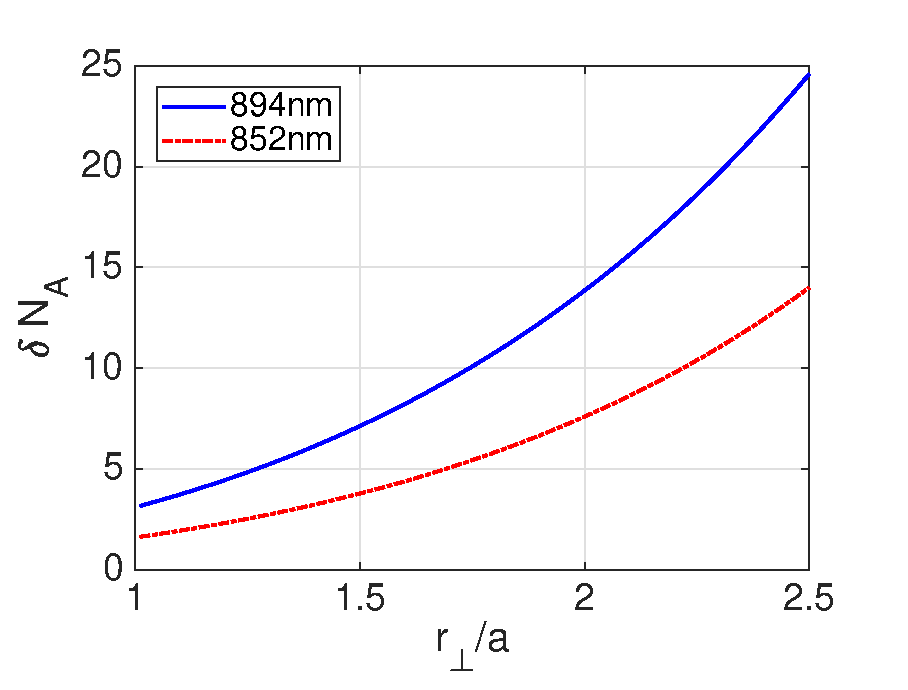
\includegraphics[scale=0.45]{../media/Figs/deltaNA_D12_r1to2d5a}}
\end{minipage}
\begin{minipage}{.48\linewidth}
\centering
\subfloat[]{\label{fig:A_D12_n1d4469_a225nm_rp}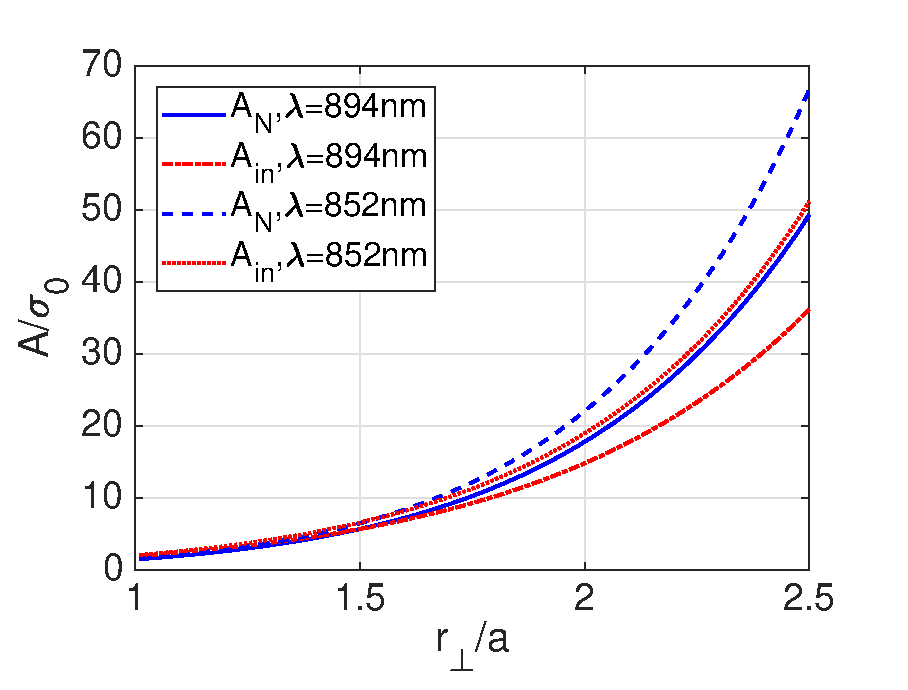
\includegraphics[scale=0.45]{../media/Figs/ANAin_D12_r1to2d5a}}
\end{minipage}
\caption[Minimum detectable atom number and mode areas as functions of the atom radial position, $ r\!_\perp/a $, when the D1- and D2-line probe lasers are used.]{Minimum detectable atom number (a) and mode areas (b) as functions of the atom radial position, $ r\!_\perp/a $, when the D1- and D2-line probe lasers are used. The group indices of refraction are $ n_g=1.4737 $ and $ n_g=1.4974 $ for the D1 ($ \lambda=894 $ nm) and D2 ($ \lambda=952 $ nm) lines, respectively. }\label{fig:AminNA_D12_n1d4469_a225nm_rp}
\end{figure}

In practice, loss and decoherence limit the atom-number resolution~\cite{dawkins_dispersive_2011, zhang_collective_2012}. 
The experimental implementation reported by Dawkins \emph{et al.}~\cite{dawkins_dispersive_2011} implies a resolution of a few tens of atoms for $ 200\sim 1000 $ trapped atoms.  
A similar experiment based on a two-color QND measurement in a nanofiber geometry was recently carried out by \emph{B\'{e}guin et al.} \cite{beguin_generation_2014} to squeeze the uncertainty in the number of trapped atoms. They achieved an atom number uncertainty of $\delta N_A = 8$ for $N_A\sim2500$ atoms, well below standard quantum limit, $\delta N_A=\sqrt{N_A}$.



	%===================QND spin squeezing=====================%
	\subsection{Collective spin squeezing via QND measurement}

The same birefringent interaction, \erf{Eq::GenHamiltonian}, can be utilized in a QND measurement to squeeze the projection noise of the collective atomic spin.  We consider squeezing of the uncertainty associated with the ``clock states" of cesium\index{state!clock state}, $\ket{\uparrow} = \ket{6S_{1/2}, f=4, m_f=0}$ and $\ket{\downarrow} = \ket{6S_{1/2}, f=3, m_f=0}$, which define a pseudospin within each atom and associated Pauli operators $\{\hat{\sigma}_x, \hat{\sigma}_y, \hat{\sigma}_z\}$.  The quantum uncertainty in the collective pseudospin,
	\begin{align}
		\jz = \frac{1}{2} \sum_{n=1}^{N_A} \hat{\sigma}_z^{(n)},  
	\end{align}
fundamentally limits the precision of atomic clocks \cite{wineland_spin_1992}. For atoms prepared in a spin coherent state (SCS) the projection noise, $\varz \big|_{\scs} = N_A/4$, sets the standard quantum limit for spin measurements. A spin squeezed state (SSS) exhibits reduced fluctuations, $ \varz \big|_{\rm SSS}  < N_A/4$, due to negative pairwise correlations between the atoms \cite{kitagawa_squeezed_1993}. Spin squeezing is typically quantified with the metrological squeezing parameter defined by Wineland \emph{et al.} \cite{wineland_spin_1992},
	\begin{align} \label{Eq::SqueezingParameter}
		\xi^2 \equiv N_A \frac{ \varz }{ \expt{\hat{J}_{||}}^2 },
	\end{align}
where $\expt{\hat{J}_{||}}$ is the mean collective spin along the direction of spin polarization. 

The clock states\index{state!clock state} are defined to have zero projection of angular momentum with respect to a bias magnetic field that defines a quantization axis, $\mathbf{e}_{\tilde{z}}$.  
Within the clock-state subspace the rank-1 vector light shift in the dispersive Hamiltonian, \erf{Eq::GenHamiltonian}, vanishes since $\bra{\uparrow}\hat{f}_k \ket{\uparrow} =\bra{\downarrow}\hat{f}_k \ket{\downarrow} = 0$ for any direction of the spin, $k$, and any quantization axis, $\mathbf{e}_{\tilde{z}}$. 
Furthermore, as shown below, atoms on either side of the nanofiber experience the same birefringent coupling. 
The resulting Hamiltonian, restricted to the clock subspace, couples the guided field of the nanofiber to the $J_z$-component of the collective pseudospin. The interaction has contributions from both the scalar and tensor light shifts,
	\begin{align} \label{Eq::ClockHamiltonian}
		\hat{H}_{J_z} = \hbar \Big\{ & \big[ \big( \chi_{H,\uparrow} +\chi_{V,\uparrow} \big) - \big( \chi_{H,\downarrow} + \chi_{V,\downarrow}\big) \big] \jz \hat{S}_0(t) \\
		+ & \big[  \big( \chi_{H, \uparrow} - \chi_{V,\uparrow} \big) - \big(\chi_{H,\downarrow} - \chi_{V,\downarrow} \big) \big]  \jz \hat{S}_1(t) \Big\}, \nonumber
	\end{align}
where the coupling strength between an atom in the clock subspace and a photon with polarization $p = \{H,V\}$ is
	\begin{equation} \label{Eq::ClockCouplingStrength}
		\chi_{p,f} \equiv - 2\pi k_0 n_g  | \mathbf{u}_p(\mbf{r}_\perp)|^2 \bra{f,0}\hat{\alpha}_{pp}  \ket{f,0},
	\end{equation}
and $f = \{4,3\}$ labels $\{\uparrow,\downarrow\}$.  
The diagonal terms in the polarizability tensor are the same for atoms at positions above and below the nanofiber, and thus all atoms contribute equally. 
In addition, a constant birefringence proportional to $ \hat{J}_0\hat{S}_1 $ is neglected here as it can be canceled with a compensating waveplate. 
Finally, the first term in \erf{Eq::ClockHamiltonian} does not affect polarization spectroscopy, but will act to rotate the pseudo-spin around the $J_z$ axis of the generalized Bloch sphere proportional to classical intensity fluctuations.
While this does not affect the squeezing of projection noise in $\hat{J}_z$, it affects the metrologically relevant squeezing by adding uncertainty to the direction of the mean spin.  By choosing a ``magic frequency" at which the light shifts on the two clock states\index{state!clock state} are equal, 
	\begin{align} \label{Eq::MagicWavelengthCondition}
		\chi_{H,\uparrow} +\chi_{V,\uparrow}  = \chi_{H,\downarrow} + \chi_{V,\downarrow},
	\end{align}
this term can be canceled \cite{chaudhury_continuous_2006}, where we have ignored the imaginary part of the coupling strengths in the dispersive regime.
Using the D1-line of $^{133}$Cs atoms as the probe light, there are two magic-frequency solutions, $ \magic{3} $ and $\magic{4}$, shown in \frf{Fig::CouplingStrength}(a).  

Because the guided probe light at the position of the atom will generally be elliptical, the light-shift interaction coherently couples different magnetic sublevels in a given manifold $f$, and thus does not conserve $\hat{J}_z$.  For example, the ellipticity of the probe light leads to a fictitious magnetic field proportional to $i \mathbf{E}^{(-)}_{\inp}(\br') \times \mathbf{E}^{(+)}_{\inp}(\br')$ that causes a precession of the spin within hyperfine manifold $f$.  This can be mitigated by a sufficiently strong bias magnetic field compared to the fictitious field \cite{smith_continuous_2004}. 


%========= FIGURE: Geometry (coupling strength, magic wavelength, area and detuning) =========%
\begin{figure}[!htbp]
\centering
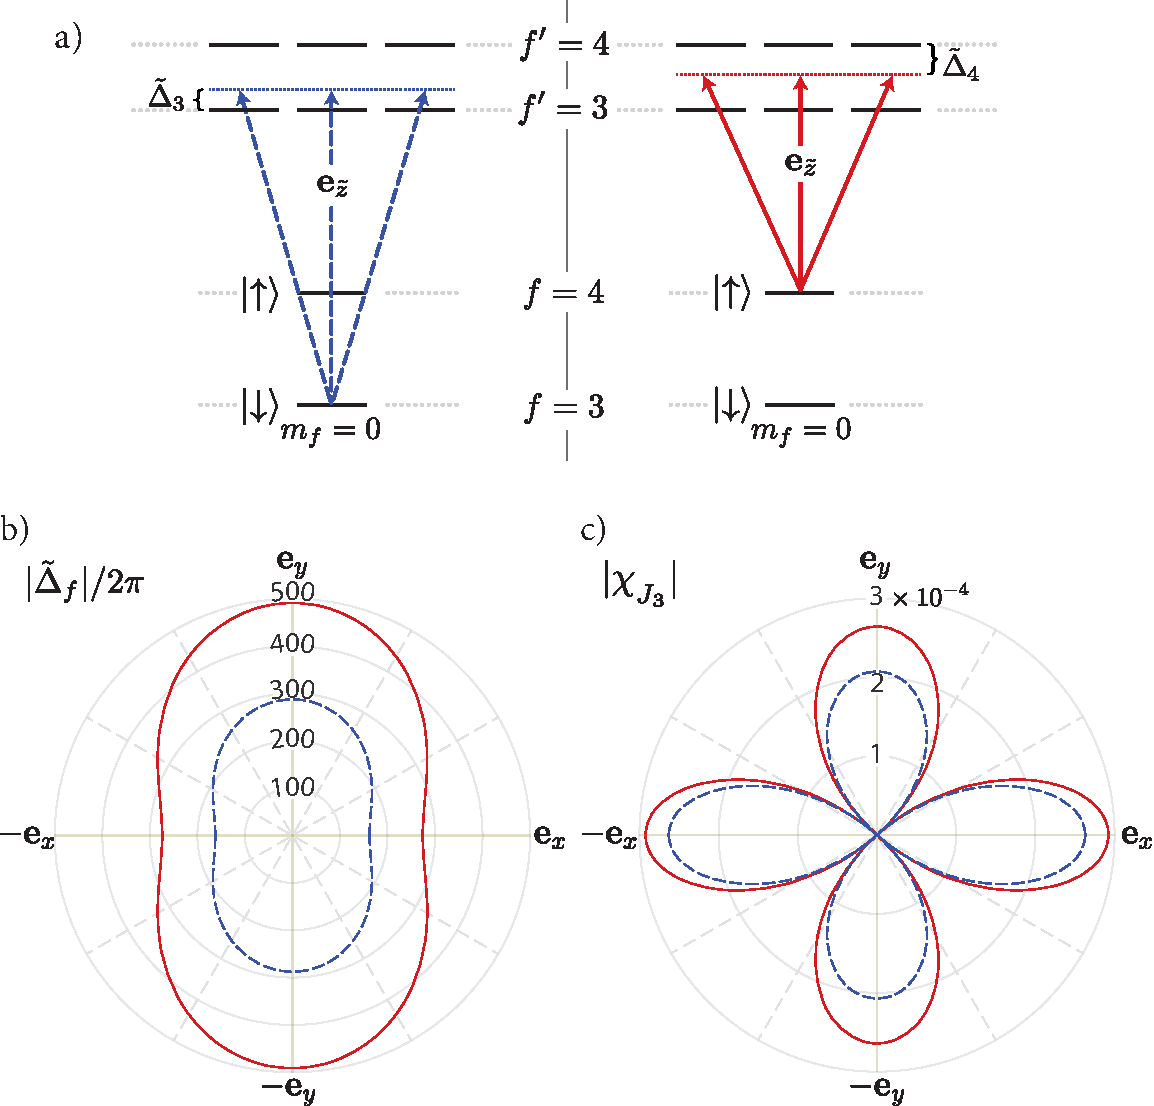
\includegraphics[scale=0.64]{../chap4/Fig3}
\caption[Parameters of the atom-light interface using the clock states of $^{133}$Cs and magic frequencies.]{Parameters of the atom-light interface using the clock states of $^{133}$Cs.  
(a) Energy level structure for atoms probed with one of two magic frequencies on the D1-line. 
(b) Magnitude of the magic detunings at which the clock states are equally light-shifted, $| \tilde{\Delta}_{f}|/2\pi \equiv | \omega_0 - \magic{f} |/2\pi$ (in units of MHz). There are two solutions shown as blue (dashed) and red lines. (c) The coupling strength, as measured by the magnitude of the polarization rotation angle on the Poincar\'{e} sphere, $|\chi_{_{ J_z}}|$, for an atom trapped in the $x$-$z$ plane at a distance $ r'\!_\perp=1.8a $ from the fiber center.  In both (b) and (c) we plot the parameter as the direction of the clock-state quantization axis is varied in the $x$-$y$ plane, for the two possible choices of magic detunings.
See text for details.}\label{Fig::CouplingStrength}
\end{figure}
%=============================================


The remaining QND interaction Hamiltonian is
	\begin{equation} \label{Eq::FaradayHam}
		\hat{H}_{J_z} = \hbar \chieff \jz \hat{S}_1(t),
	\end{equation}
where the rotation angle on the Poincar\'{e} sphere at the magic wavelength is,
\begin{equation}\label{eq:chiJ3}
\chieff = \big( \chi_{H, \uparrow} - \chi_{V,\uparrow} \big) - \big(\chi_{H,\downarrow} - \chi_{V,\downarrow} \big) = 2(\chi_{H, \uparrow}-\chi_{H, \downarrow}).
\end{equation}
In the standard way, squeezing the uncertainty in $\jz$ by QND measurement can be generated by preparing the atoms in a SCS along $\jx$, passing a probe prepared along $\hat{S}_2$ with photon flux $\dot{N}_L$, and continuously monitoring the $S_3$-component of the guided light in a polarimeter. The measurement strength,
	\begin{align} \label{Eq::MeasurementStrength}
		\kappa \equiv |\chieff|^2 \dot{N}_L, 
	\end{align}
quantifies the rate at which we squeeze projection noise, with $\chieff$ given in \erf{eq:chiJ3}. 
In the absence of any decoherence, such a QND measurement for integration time $T$ squeezes the initial uncertainty in $\jz$ according to $(\Delta J_z^2)_{\rm out}= (\Delta J_z^2)_{\rm in}/(1+r)$, where
	\begin{equation}
		r = \kappa T  (\Delta J_z^2)_{\inp}
	\end{equation}
is the integrated measurement strength \cite{hammerer_quantum_2010, baragiola_three-dimensional_2014}.

The strength of the birefringent interaction arises from two fundamental sources.  The anisotropy of the   $H$ and $V$ polarized modes leads to a polarization-dependent index of refraction, as described in Sec.~\ref{Sec::AtomNumberMeasurement}.  In addition there is a dependence of the atom-photon coupling on the internal spin state of the atom due to the atomic tensor polarizability.  In particular, we are interested in the dependence on the two clock states of the atom.  This spin-dependent coupling will depend on the choice of quantization axis that defines the clock state\index{state!clock state} with projection $m_f=0$. 

We combine these two effects and obtain a compact expression for the coupling strength $\chieff$ using the irreducible tensor decomposition of the atomic polarizability, \erf{Eq::PolarizabilityIrrep}.  
Let $\{\mathbf{e}_{\tilde{x}},\mathbf{e}_{\tilde{y}}, \mathbf{e}_{\tilde{z}}\}$ be a space-fixed Cartesian coordinate system, where $\mathbf{e}_{\tilde{z}}$ defines the quantization axis of the atom, set by the magnetic field.  Because of the azimuthal symmetry of clock state around the $\qaxis$ axis, the polarizability tensor is diagonal in that basis.  
Noting that $\langle f,0 | \hat{f}_{\tilde{z}}| f,0 \rangle =0$ and $\langle f,0 | \hat{f}_{\tilde{x}}^2| f,0 \rangle = \langle f,0 | \hat{f}_{\tilde{y}}^2| f,0 \rangle = \langle f,0 | \hat{\mathbf{f}}^2| f,0 \rangle /2 =f(f+1)/2$, it follows that the expectation value of the irreducible rank-2 component of the atomic polarizability is
	\begin{align} \label{Eq::CouplingAngleMagic}
		\langle f,0 | \poltens \phantom{}^{(2)}| f,0 \rangle = \sum_{f'} \charpol C^{(2)}_{ff'} \frac{f(f+1)}{6} \Big( \unittens - 3\qaxis \otimes \qaxis \Big).
	\end{align}
The combined scalar and tensor light shifts yield a coupling strength, \erf{Eq::ClockCouplingStrength},
	\begin{align}
		\chi_{p,f} &  = n_g \sigma_0 \big(  a_{f} \left|\mathbf{u}_p(\br'_\perp)\right|^2 - b_{f} \left|\mathbf{e}_{\tilde{z}} \cdot \mathbf{u}_p(\br'_\perp)\right|^2 \big), \label{Eq::ClockStateCoupling}
	\end{align}
with coefficients that depend on detunings and atomic structure,
	\begin{align}
		a_f &= \sum_{f'}  \Big(C^{(0)}_{ff'} + \frac{f(f+1)}{6} C^{(2)}_{ff'} \Big) \frac{\Gamma}{4 \Delta_{ff'}},\\
		b_f &= \frac{f(f+1)}{2}\sum_{f'} C^{(2)}_{ff'}  \frac{\Gamma}{4 \Delta_{ff'}}.
	\end{align}
At the magic wavelength set by \erf{Eq::MagicWavelengthCondition},
\begin{equation}
	\frac{a_4-a_3}{b_4-b_3} =  \frac{ |\mathbf{e}_{\tilde{z}} \cdot \mathbf{u}_V(\br'_\perp)|^2  + |\mathbf{e}_{\tilde{z}} \cdot \mathbf{u}_H(\br'_\perp) |^2 }{ |\mathbf{u}_H(\br'_\perp)|^2 + |\mathbf{u}_V(\br'_\perp)|^2 },
\end{equation}
which depends on the choice of quantization axis. Note that, in Appendix~\ref{chap:magicwavelength}, we prove the magic wavelengths can be found only if we utilize the tensor polarizability of atoms and design some multi-color schemes for the QND measurement and spin squeezing. We will not discuss the details in the main text here.

We write the effective rotation angle in the Hamiltonian, \erf{Eq::FaradayHam}, as
	\begin{align} \label{Eq::chieff}
		\chieff = \frac{\sigma_0}{A_{J_z}} \frac{\Gamma}{ 2 \Delta_{J_z}},
	\end{align}
with an ``effective detuning" set by the magic-wavelength condition,
	\begin{align} \label{Eq::SqueezingEffectiveDetuning}
		 \Delta_{J_z}^{-1} \equiv \frac{4}{\Gamma} (b_4 - b_3) =   \sum_{f'}  \left( C^{(2)}_{4f'}\frac{10}{\Delta_{4f'}} -  C^{(2)}_{3f'}\frac{6}{ \Delta_{3f'} } \right),
	\end{align}
and an effective area given by
	\begin{align} \label{Eq::SqueezingModeArea}
		A_{J_z}^{-1} & = n_g \frac{ |\mathbf{e}_{\tilde{z}} \cdot \mathbf{u}_V(\br'_\perp)|^2 |\mathbf{u}_H(\br'_\perp)|^2 - |\mathbf{e}_{\tilde{z}} \cdot \mathbf{u}_H(\br'_\perp) |^2 |\mathbf{u}_V(\br'_\perp)|^2 }{ |\mathbf{u}_H(\br'_\perp)|^2 + |\mathbf{u}_V(\br'_\perp)|^2 } 
	\end{align}	
We see here the explicit dependence of the coupling strength on both the anisotropy of the modes and on the tensor atomic response, which in turn depends on a particular choice of clock states\index{state!clock state}.  The quantization axis that maximizes $\chieff$ is that which minimizes $A_{J_z}$ at a given magic detuning.  
Since the $z$-component of the guided modes is $90^\circ$ out-of-phase with the transverse components, the quantization axis maximizing the atom-light coupling is specified by an angle in the transverse $x$-$y$ plane, $\varphi$,
	\begin{align} \label{Eq::QuantizationAxis}
		\qaxis = \cos \varphi \mbf{e}_x + \sin \varphi \mbf{e}_y.
	\end{align}
The dependence of the magic detunings on the direction of quantization axis is shown in \frf{Fig::CouplingStrength}(b) for atoms trapped at a typical distance of $r_\perp'=1.8a$ on the $x$ axis.   
In typical operating regimes, the magic frequencies are hundreds of MHz from resonance with either excited state, placing the interaction in the off-resonant, dispersive regime.  
Using these magic detunings, in \frf{Fig::CouplingStrength}(c) we show the variation in $\chieff$ as a function of $\varphi$.  
This suggests that, based solely on the strength of the coherent interaction, the $x$ axis is the optimal quantization axis. 
As we will see in the next section, the optimal quantization axis is significantly modified when decoherence due to optimal pumping is included.


	%====== SUBSECTION: Including optical pumping ======%
	\subsection{Decoherence due to optical pumping}\label{sec:decoherence}
	
The treatment above considers an idealized QND interaction. 
The coupling of the atoms to the probe, however, will always lead to scattering of photons into modes other than the forward-scattered guided mode.  
This is accompanied by optical pumping that destroys the entanglement associated with spin squeezing.  In addition it reduces the metrologically useful signal.  
The maximum achievable metrologically relevant squeezing is determined by the balance of this decoherence with the QND measurement. 

We model this using a first-principles stochastic master equation description (SME)~\cite{jacobs_straightforward_2006, baragiola_three-dimensional_2014},
	\begin{align} \label{Eq::SME}
		d \hat{\rho} = s\sqrt{\frac{\kappa}{4}} \mathcal{H}[\hat{\rho}] dW + \frac{\kappa}{4} \mathcal{L}[\hat{\rho}] dt + \sum_n \mathcal{D}_n [\hat{\rho}] dt,
	\end{align}
where $s = {\rm sign}(\chieff)$ and $\hat{\rho}$ is the collective atomic state. 
The measurement strength $\kappa =|\chieff|^2 \dot{N}_L$ determines the rate of the spin squeezing in the absence of decoherence.  
The first two terms describe the QND measurement, where $dW$ is a stochastic Weiner increment satisfying $dW^2 = dt$. 
The conditional dynamics that result from the measurement are generated by the superoperator
	\begin{align}
		\mathcal{H}[\hat{\rho}] = \jz \hat{\rho} + \hat{\rho} \jz - 2 \expt{\jz} \hat{\rho},
	\end{align}
and the collective Lindblad map is
	\begin{align}
		\mathcal{L}[\hat{\rho}] = - \smallfrac{1}{2} \big( \hat{\rho}  \jz^2 + \jz^2 \hat{\rho} \big) + \jz \hat{\rho} \jz.
	\end{align}
The final term in \erf{Eq::SME} describes the effect of optical pumping acting locally on each atom along the nanofiber. 

The optical pumping map is governed by a standard master equation~\cite{Deutsch2010a}.  
Restricting to the two-dimensional subspace associated with the clock states\index{state!clock state}, the action on the $n^{th}$ atom is
	\begin{align}
		\mathcal{D}_n[\hat{\rho}] =  \sum_{f=3,4} \Big\{& -\frac{\gamma_{f}}{2} \big[ \hat{\rho} (\op{f,0}{f,0})^{(n)} + (\op{f,0}{f,0})^{(n)}\hat{\rho} \big]\\
		&+  \sum_{\tilde{f} =3,4}  \gamma_{f \rightarrow \tilde{f}}(\op{\tilde{f},0}{f,0})^{(n)} \hat{\rho}(\op{f,0}{\tilde{f},0})^{(n)} \Big\}.\nonumber
	\end{align}
Here, $\gamma_{f}$ is the total rate of photon scattering by atoms in state $\ket{f,0}$ and  $\gamma_{f \rightarrow \tilde{f} }$ is the rate of optical pumping between the clock states, $\ket{f,0} \rightarrow \ket{\tilde{f},0}$ (see Appendix~\ref{Appendix::Rates}). Expressed in terms of Pauli operators on the clock-state pseudospin, the map acts as
	\begin{align} \label{Eq::OpticalPumpingMapSchr}
		\mathcal{D}_n [\hat{\rho}] 
				=& - \!\bigg[ \frac{2(\gammau \!+\! \gammad) \!-\! \gammauu \!-\! \gammadd}{4} \bigg] \hat{\rho} \!-\! \frac{ \gammau \!-\! \gammad \!-\! \gammauu \!+\! \gammadd }{4} \big( \hat{\sigma}_z^{(n)} \hat{\rho}\!+\! \hat{\rho} \hat{\sigma}_z^{(n)} \big) \nn \\
		&+ \frac{\gammauu+\gammadd}{4} \hat{\sigma}_ 3^{(n)}\hat{\rho} \hat{\sigma}_z^{(n)} + \gammaud  \hat{\sigma}_-^{(n)} \hat{\rho} \hat{\sigma}_+^{(n)} + \gammadu  \hat{\sigma}_+^{(n)} \hat{\rho} \hat{\sigma}_- ^{(n)}.   
	\end{align} 
There are three important features of this map that are not typical in a QND measurement of ideal spin-$\half$ particles.  
First, the map is not trace preserving because atoms can be pumped out of the clock states\index{state!clock state}. 
Second, unequal rates of optical pumping for $\ket{\uparrow}$ and $\ket{\downarrow}$ polarize the mean $\expt{\jz}$ towards a value different from that found in the QND measurement. 
Third, owing to the large ground hyperfine splitting, photons arising from optical pumping of $f \rightarrow \tilde{f}=3$ and $f \rightarrow \tilde{f}=4$ are distinguishable, thus these processes destroy coherences between $\ket{\uparrow}$ and $\ket{\downarrow}$. 

We calculate the squeezing parameter as a function of time based on the evolution of atomic correlation functions, where operators evolve according to the adjoint form of the SME in \erf{Eq::SME}.  The collective atomic variables obey the following stochastic equations of motion (see Appendix \ref{Appendix::OpticalPumping}),
\begin{subequations}\label{Eq::collectivedynamics}
	\begin{align} 
		&d N_C = -\gamma_{00} N_C dt + 2\gamma_{03} \expt{\hat{J}_z} dt \label{Eq::NA}\\
		&d \expt{\hat{J}_x}  = -\gamma_{11} \expt{\hat{J}_x} dt , \label{Eq::MeanSpinDecay} \\
		&d \expt{\hat{J}_z}  = s\sqrt{\kappa} \varz dW -\gamma_{33} \expt{\hat{J}_z}dt + \smallfrac{1}{2}\gamma_{30} N_C dt,   \\
		&d \varz  = \!- \kappa \big(\varz\big)\!^2\! dt\!-\! 2 \gamma_{33} \varz dt \!\!+\! \smallfrac{1}{4} \!\big( 2\gamma_{33}\!\!-\!\!\gamma_{00} \!\big) N_C dt \!\!+\! \smallfrac{1}{2} \big( \gamma_{03} \!\!-\!\! 2 \gamma_{30} \big)\! \expt{\!\hat{J}_z\!} dt,   \label{Eq::varJz} 
	\end{align}
\end{subequations}
where the decay and feeding rates are given in \erf{Eq::DecayRates}.
The total number of atoms in the clock-state subspace is given by $N_C$, which primarily decays at rate $\gamma_{00}$. 
The final term in \erf{Eq::varJz}, proportional to $\expt{\hat{J}_z}$, is typically negligible since in most applications $\expt{\hat{J}_z} \ll N_C$.  
We retain this small correction since unbalanced optical pumping acts to polarize the atoms and alters the rate of atom loss.  

To find the peak squeezing in the presence of optical pumping, we numerically integrate Eqs. (\ref{Eq::NA}--\ref{Eq::varJz}) and then use \erf{Eq::SqueezingParameter} to calculate the metrological squeezing parameter, $\xi^2$, as a function of time. 
We choose here the magic frequency close to the $ f=4\leftrightarrow f'=4 $ transition, $ \magic{4} $, which is furthest from resonance with both excited hyperfine transitions. 
Typical time evolution is shown in \frf{Fig::Squeezing_Dynamics} for $2500$ atoms trapped a distance $r'\!_\perp=1.8a$ from the center of the nanofiber, where time is scaled to the characteristic scattering rate, 
\begin{align}\label{Eq::gamma_s}
\gamma_s \equiv \frac{\sigma_0}{A_{\rm in}}\frac{\Gamma^2}{4 \Delta_{J_z}^2} \dot{N}_L .
\end{align}  
We study the dynamics for two choices of quantization axis: (i) along the $x$ axis and (ii) along the numerically determined optimal axis.  Figure \ref{Fig::Squeezing_Dynamics}(a) shows the time evolution of the squeezing parameter.  We achieve a maximum squeezing of 4.7 dB when the clock states are chosen along the optimal axis; $\qangle_{\rm opt} \approx 86^\circ$ in \erf{Eq::QuantizationAxis}. 

%========= SQUEEZING DYNAMICS: \xi, variance, mean,  N_A =========
\begin{figure*}[tbp]
\centering
\hspace{-50pt}
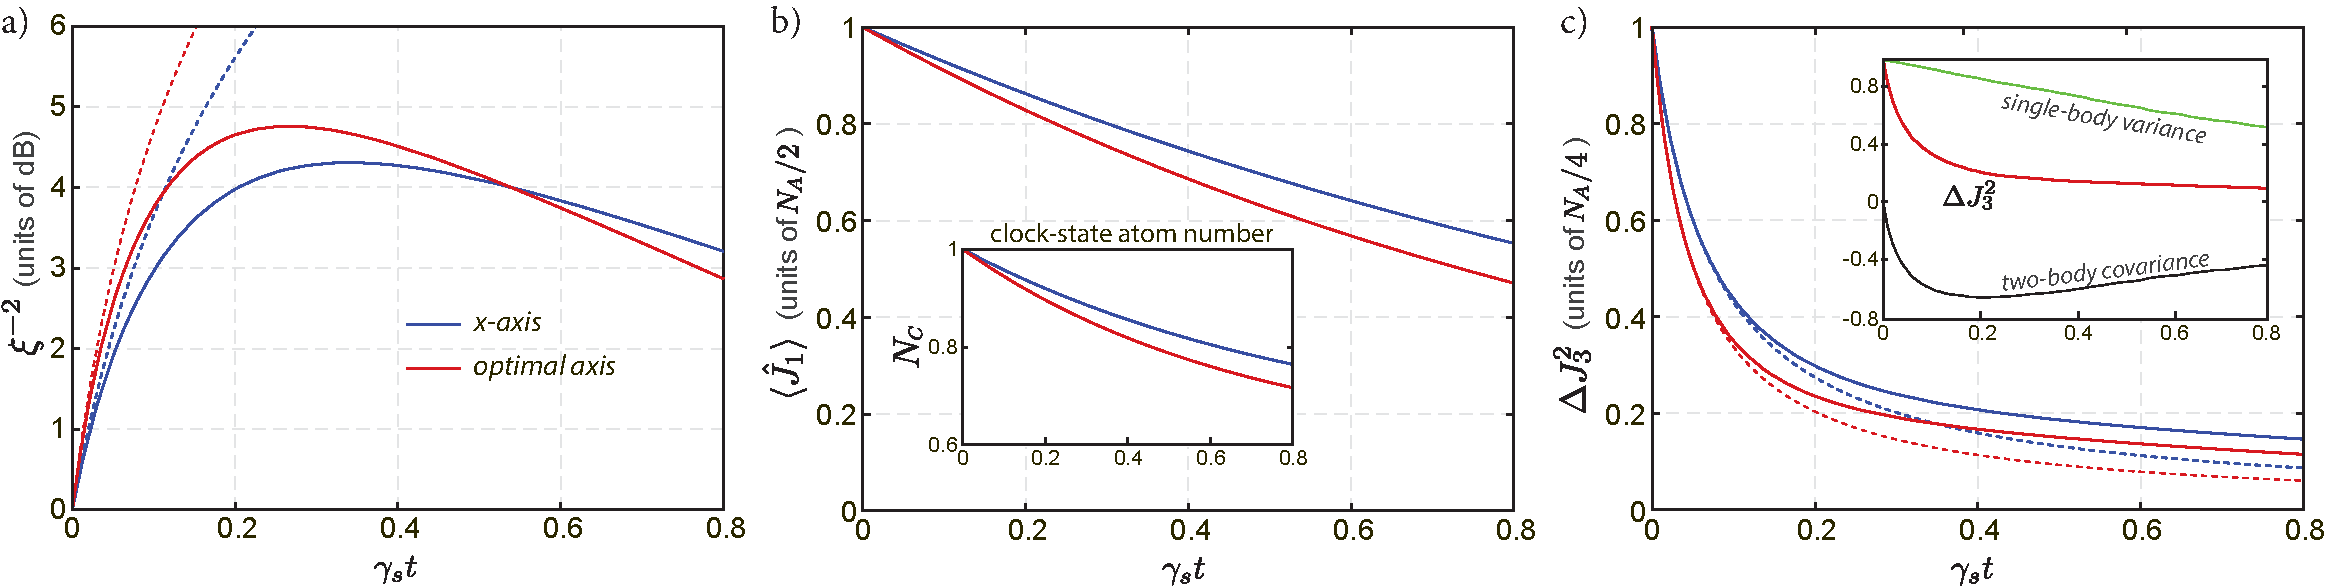
\includegraphics[scale=0.42]{../chap4/Fig4}
\caption[Squeezing on the clock states as a function of time in units of the scattering rate $\gamma_s$ for $2500$ atoms trapped in the $x$-$z$ plane at a distance $ r'\!_\perp=1.8a$ from the axis of the nanofiber.]{Squeezing on the clock states as a function of time in units of the scattering rate $\gamma_s$ for $2500$ atoms trapped in the $x$-$z$ plane at a distance $ r'\!_\perp=1.8a$ from the axis of the nanofiber. The optimal quantization axis (red) is compared to the quantization along the $x$ axis (blue). 
Dashed lines indicate simulations without optical pumping; i.e. no decoherence. 
(a) Metrological spin squeezing parameter $\xi^{-2}$, \erf{Eq::SqueezingParameter}, in dB. 
(b) Collective mean spin $\expt{\hat{J}_1}\equiv \expt{\hat{J}_x}$ and decaying atom number in the clock states, $N_C$ (inset).
(c) Conditional squeezed variance $\varz$. 
The inset shows the decomposition at the optimal quantization axis of $ \Delta J_3^2\equiv \Delta J_z^2 $ (red dashed) into the single-body variance, $N_A (\Delta j_z^{(1)})^2$ (green) and the two-body covariance, $N_A(N_A-1)\expect{\Delta j_z^{(1)}\Delta j_z^{(2)}}$ (black), as given by \erf{Eq::VarianceDecomposition}.
}\label{Fig::Squeezing_Dynamics}
\end{figure*}
%================


The peak squeezing is ultimately limited by the combined effects of optical pumping on both $\expt{\jx}$ and $\varz$.  Here, as in a free-space model \cite{baragiola_three-dimensional_2014}, the primary factor that limits metrological squeezing is the decay of the collective mean spin $\expt{\jx}$. 
A scattered photon eliminates the initial coherence between $\ket{\uparrow}$ and $\ket{\downarrow}$ within a single atom, thus depolarizing $\expt{\jx}$.  
Atoms optically pumped to magnetic sublevels outside of the clock subspace decay $N_C$, further reducing $\expt{\jx}$. 
These effects are captured by the depolarization rate $\gamma_{11}$ in the equation for $\expt{\jx}$, \erf{Eq::MeanSpinDecay}, whose solution is plotted in \frf{Fig::Squeezing_Dynamics}(b).
  
We can gain deeper understanding in the microscopic effects of optical pumping on spin squeezing by looking at the evolution of the one and two-body correlation functions.  In terms of its constituent pseudospins, the collective variance takes the form
	\begin{align} \label{Eq::VarianceDecomposition}
	\varz & = N_A \big( \Delta j_z^{(1)} \big)^2 + N_A(N_A-1) \expt{ \Delta j_z^{(1)} \Delta j_z^{(2)} }
	\end{align}
for permutationally symmetric states considered here, where $(1)$ and $(2)$ label any two atoms in the ensemble. Loss of atoms affects the first (single-body) variance term, which scales as $N_A$.
The two-body correlations which contribute as $N_A^2$ to the collective fluctuations, 
	\begin{align}
		\expt{ \Delta j_z^{(1)} \Delta j_z^{(2)} } &\equiv \smallfrac{1}{4} \big( \expt{ \hat{\sigma}_z^{(1)} \otimes \hat{\sigma}_z^{(2)}  } - \expt{\hat{\sigma}_z^{(1)} }^2  \big).
\end{align}
have a much larger influence on the total variance. Spin-spin correlations at the heart of spin squeezing, $\expt{ \hat{\sigma}_z^{(1)} \otimes \hat{\sigma}_z^{(2)} }$, rapidly generated by the measurement backaction decohere by optical pumping according to Eqs. (\ref{Eq::TwoBodyDecay}--\ref{Eq::OperatorMap}),
	\begin{align} \label{Eq::TwoBodySpinDecay}
		\frac{d}{dt} \expt{\hat{\sigma}_z^{(1)} \otimes \hat{\sigma}_z^{(2)} }  \Big|_{\rm op} = - 2 \gamma_{33}  \expt{\hat{\sigma}_z^{(1)} \otimes \hat{\sigma}_z^{(2)}} + \gamma_{30} \expt{ \hat{\mathbbm{1}}^{(1)}_C \otimes \hat{\sigma}_z^{(2)} + \hat{\sigma}_z^{(1)} \otimes \hat{\mathbbm{1}}^{(2)}_C },
	\end{align}
where $\hat{\mathbbm{1}}^{(n)}_C \equiv \big( \op{\uparrow}{\uparrow} + \op{\downarrow}{\downarrow} \big){}^{(n)}$ is the single-body projector onto the clock states.   
In addition, atoms that return to the clock subspace after scattering a photon inject additional noise into $\varz$.  
All of these effects are included in the equation for $\varz$, \erf{Eq::varJz}, whose overall and decomposed dynamical evolutions are shown in Fig. \ref{Fig::Squeezing_Dynamics}(c). 


%========= FIGURE: Peak squeezing (\xi, measurement strength, scattering rates) =========
\begin{figure}[!htbp]
\centering
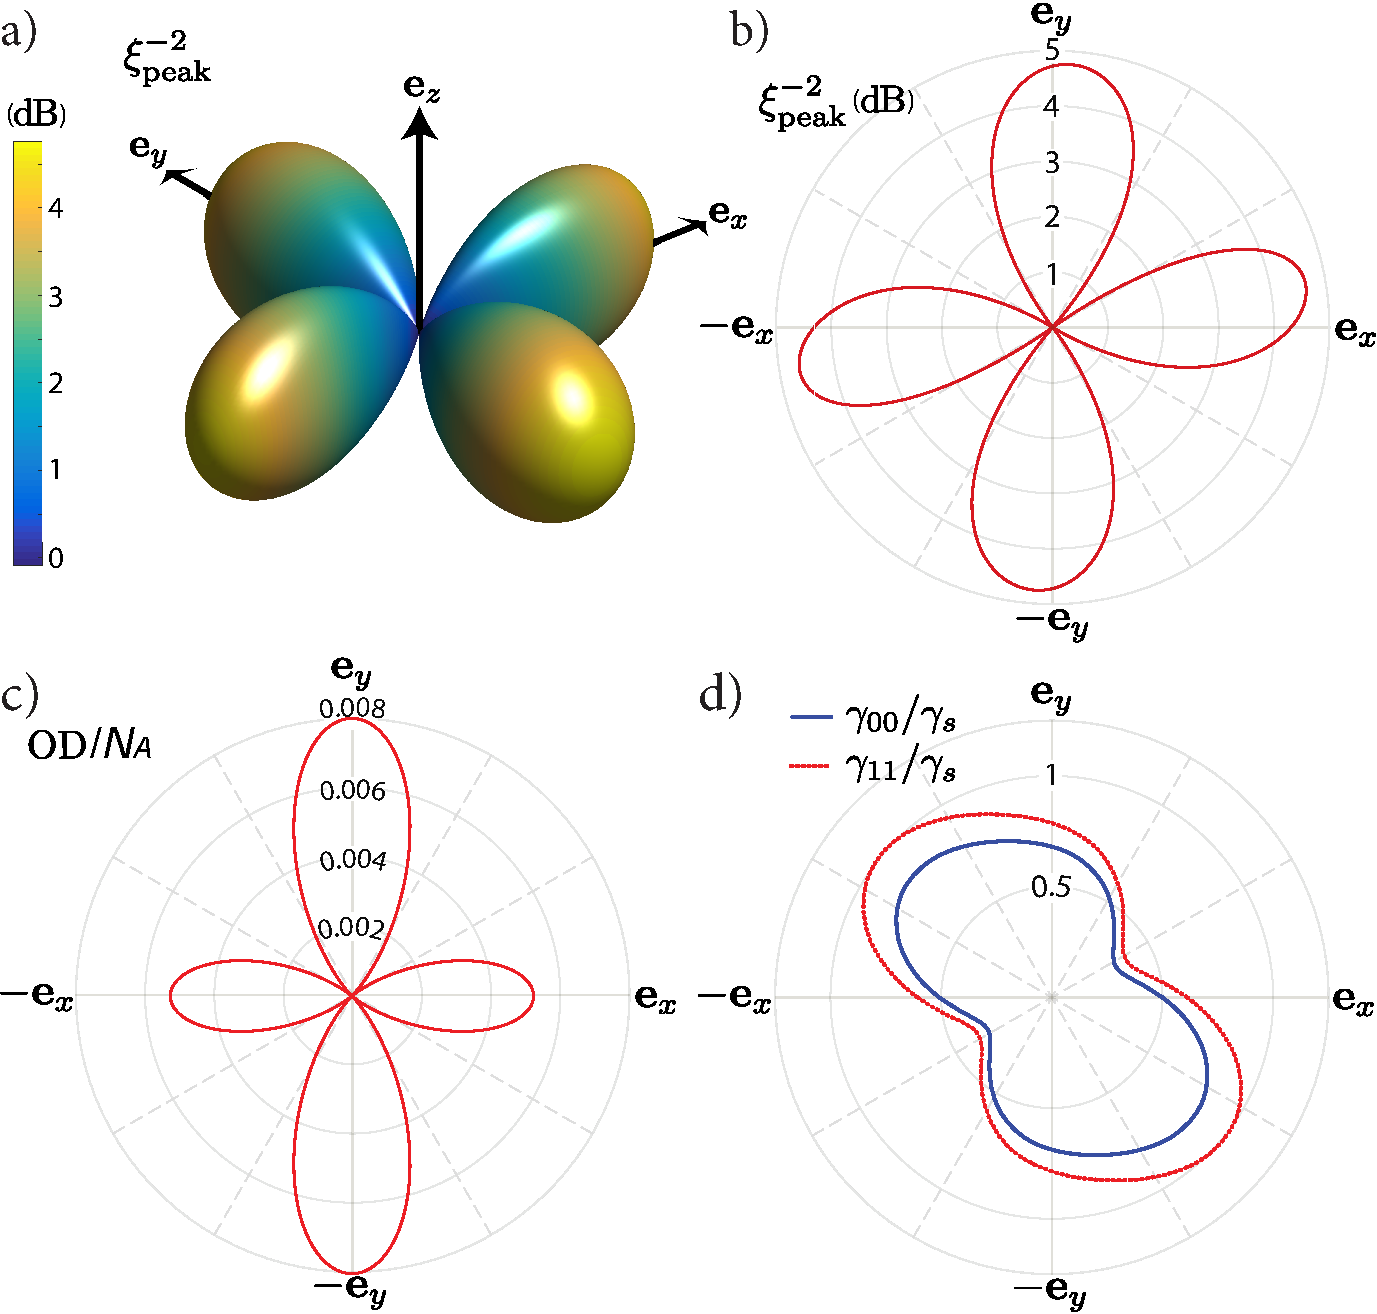
\includegraphics[scale=0.5]{../chap4/Fig5}
\caption[Dependence of the parameters that determine metrological squeezing  on the direction of the quantization axis that defines the clock states, $\mathbf{e}_{\tilde{z}}$.]{Dependence of the parameters that determine metrological squeezing  on the direction of the quantization axis that defines the clock states, $\qaxis$.  In all cases we consider $2500$ atoms trapped in the $x$-$z$ plane at distance $ r'\!_\perp=1.8a$ from the axis of the nanofiber. 
In (b--d) $\qaxis$ is confined to the $x$-$y$ plane, where the optimal peak squeezing occurs.
(a,b)  Peak achievable squeezing at the maximum time, measured in dB, as a function of the direction of  $\qaxis$. 
(c) OD/$N_A$=$\sigma_0 A_{in}/A^2_{J_z}$, \erf{Eq::OD/atom}.
(d) Rates of atom loss, $\gamma_{00}$, and depolarization, $\gamma_{11}$ relative to the characteristic scattering rate $\gamma_s$.  See Eqs.~\eqref{Eq::lrate} and~\eqref{Eq::frate}. }\label{Fig::Squeezing_QuantizationAxis}
\end{figure}
%================


With our model, we explore optimal conditions for generating spin squeezing.   The choice of quantization axis $\qaxis$ that defines clock states affects both the measurement strength and the relative rates of optical pumping. We plot the peak squeezing as a function of the direction of $\qaxis$ in the $x$-$y$ plane in \frf{Fig::Squeezing_QuantizationAxis}(b). 
We gain insight into the tradeoffs between QND entangling interaction and decoherence by independent inspection of the measurement strength and optical pumping rates.  
First, the rate of squeezing is determined by the effective optical density per atom on resonance,
\begin{align}\label{Eq::OD/atom}
\mathrm{OD}/N_A \equiv \frac{\kappa}{\gamma_s}=\frac{\sigma_0 A_{\rm in}}{A_{J_z}^2},
\end{align} 
which peaks when $\qaxis$ is along the $y$ axis, as seen in \frf{Fig::Squeezing_QuantizationAxis}(c). 
Choosing $\qaxis$ along $y$, the OD/$N_A$ is about 50\% larger than along $x$ axis.  
The various forms of decoherence similarly vary with quantization axis, as seen in \frf{Fig::Squeezing_QuantizationAxis}(d), where we plot the dominant rate of atom loss, $\gamma_{00}$, and the depolarization rate of the mean pseudospin $\expt{\jx}$, $\gamma_{11}$. 
Because the magic frequency $\magic{4}$ is nearly equidistant from $f'=3$ and $f'=4$ when the quantization  axis is near the $y$ axis (see \frf{Fig::CouplingStrength}(b)) this choice of quantization axis provides more protection from decoherence.   
While the decoherence rates in \frf{Fig::Squeezing_QuantizationAxis}(d) are largest near the $y$ axis, the increase in $\kappa$ more than compensates to provide optimal peak squeezing.

Finally, we explore the optimal conditions as a function of the trapping geometry.  
The dispersive entangling interaction is based on the collective atomic coupling to the evanescent guided-mode fields, which decay exponentially away from the nanofiber surface, as seen in OD/$N_A$ plotted in \frf{Fig::Squeezing_Distance}(a). 
From Eq.~\eqref{Eq::varJz}, the optimal choice of quantization axis depends not only on distance from the fiber but also weakly on the atom number, \frf{Fig::Squeezing_Distance}(b) because of the competition between squeezing and decoherence.  
At the optimal quantization axis, the strong dependence of peak achievable squeezing on distance from the fiber is as seen in \frf{Fig::Squeezing_Distance}(c) along with the expected increase as more atoms contribute to the atom-light interface.  

Several effects limit the reliability of the simulations for atoms trapped very near the fiber surface as $r'\!_\perp \rightarrow a$. 
First, strong van der Waals interactions modify the light shifts and magic frequencies \cite{vetsch_eugen_optical_2010, lacroute_state-insensitive_2012}.  
Second, the optical pumping model used here breaks down when the local density of states is significantly modified by the presence of the dielectric nanofiber \cite{LeKien2005a, le_kien_scattering_2006}. 
At distances $r'\!_\perp > 1.5a$ the atoms' local environment is roughly that of unmodified vacuum \cite{LeKien2005a} and a free-space optical pumping model in \erf{Eq::OpticalPumpingMapSchr} suffices. 


%======= FIG: Scaling with atom number and distance =======
\begin{figure*}[t]
\centering
\hspace{-50pt}
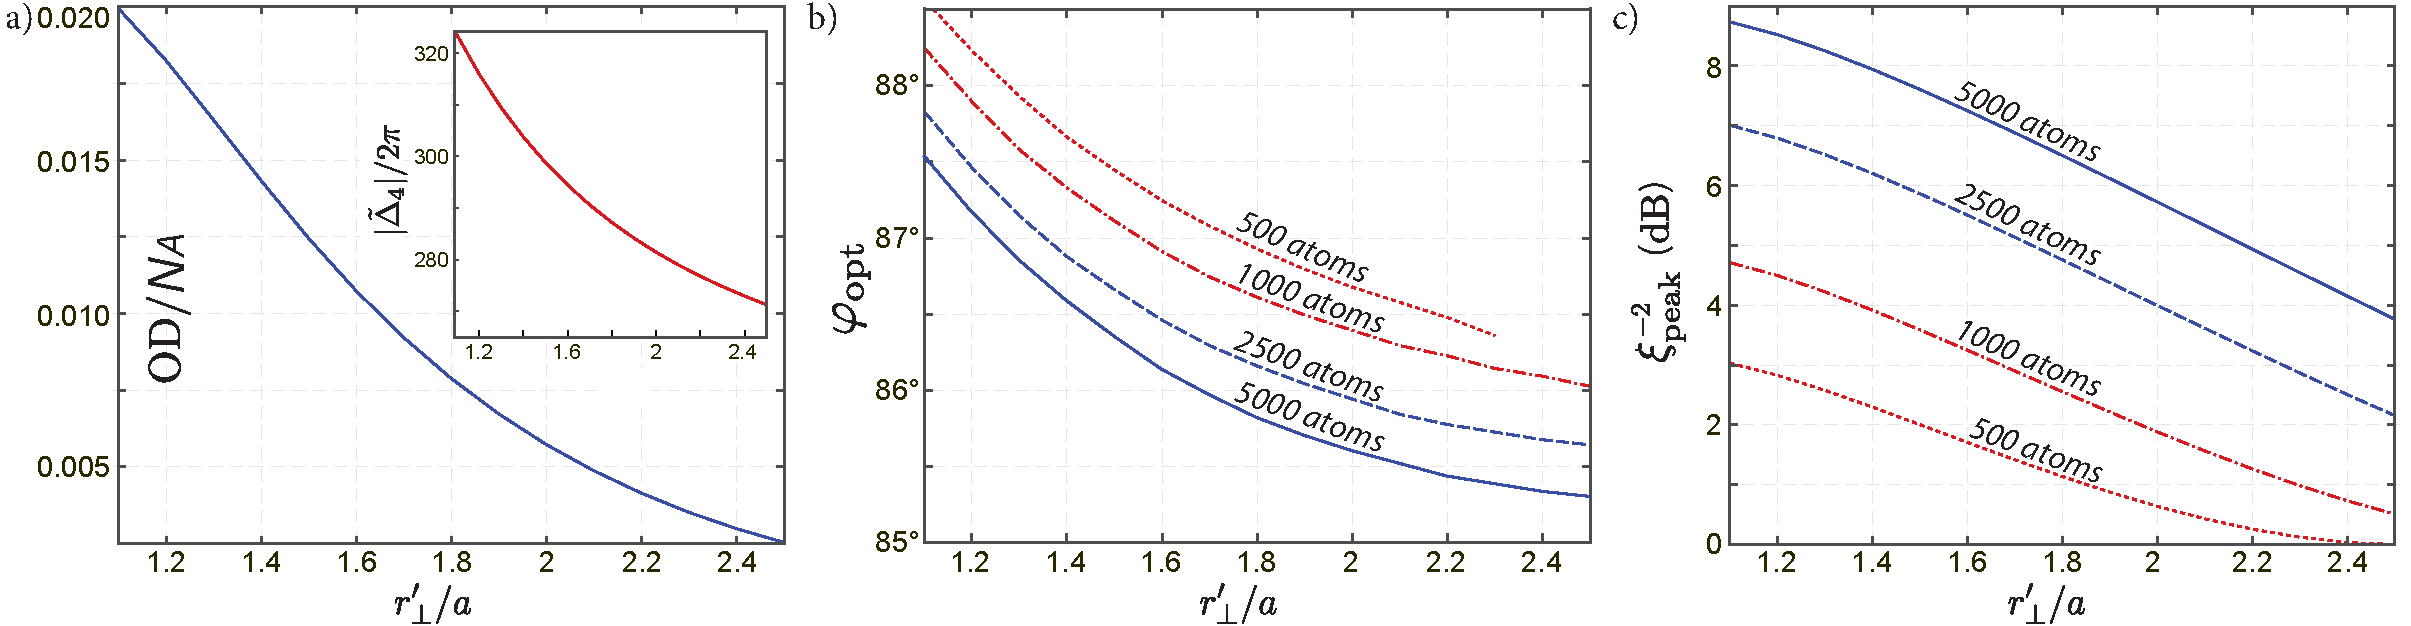
\includegraphics[scale=0.41]{../chap4/Fig6}
\caption[Parameters that define squeezing as a function of trapping distance $r'_\perp$ and initial atom number $N_A$.]{Parameters that define squeezing as a function of trapping distance $r'_\perp$ and initial atom number $N_A$. (a) OD/$N_A$. Inset is the corresponding magic detuning in units of MHz (see text).
(b) Optimal quantization axis orientation angle $\qaxis$ in the $x$-$y$ plane for different atom numbers. 
The line with $ 500 $ atoms terminates when the squeezing effect is too weak to be observed ($ r'\!_\perp>2.3a $).
(c) Peak metrological squeezing at the optimal $\qaxis$ for different atom numbers.} \label{Fig::Squeezing_Distance}
\end{figure*}
%================================


%====== SECTION: Summary and outlook ======%
\section{Summary and Outlook} \label{Sec::Conclusion}

We studied the strong cooperativity in the atom-light interface that can be achieved based on atoms trapped in the evanescent field surrounding an optical nanofiber, and interacting with a guided mode in the dispersive regime. 
The key parameter that determines the coupling is the resonant optical density per atom. 
Due to the tight confinement of the guided mode over the entire chain of atoms this parameter is $ \mathrm{OD}/N_A\sim 10^{-2} $ for typical geometries used in current experiments, which approaches that achieved for atomic ensembles trapped inside optical cavities of moderate finesse \cite{chen_conditional_2011, zhang_collective_2012}.  
In contrast, the atom-light coupling for atoms in free space is typically orders of magnitude smaller, $ \mathrm{OD}/N_A \sim 10^{-6}$.  
Under ideal conditions the atom-light interaction is entirely symmetric along the nanofiber, providing a platform for long-range correlations independent of distance between the atoms. 
As the light is entirely guided, fiber- or waveguide-coupled atomic ensembles can be networked together or coupled to other physical systems in a hybrid platform \cite{hafezi_atomic_2012, liebermeister_tapered_2014, Meng2015nanowaveguide, Tiecke2015Efficient} for truly long-range entanglement generation and distribution. 

We calculated the dispersive response based on a modal decomposition of the dyadic Green's function, which provides a general method to calculate the induced phase shifts and polarization rotations of the guided modes. 
With this we studied the QND measurement of atoms via polarization spectroscopy. 
In particular, we studied squeezing of the collective pseudospin associated the atomic clock states of cesium. 
The atoms induce a birefringent index of refraction on the light, conditional on the spin state, which provides a mechanism for measuring the atomic spin projection and thus squeezing its uncertainty.  
Based on our formalism we calculated the nanofiber-enhanced measurement strength that determines the rate of squeezing.  

The peak squeezing one can generate depends on a detailed balance between the reduction of spin projection noise based on QND measurement and the damage done to the spin ensemble due to optical pumping.  
Both measurement and optical pumping arise from the same physical mechanism -- scattering of photons by atoms.  
The former corresponds to cooperative forward scattering into the guided mode whereas the latter corresponds to local scattering into all other modes, primarily the unguided ``radiation" modes.   The cooperativity, specified by the effective OD/$N_A$, determines the ratio of these two effects and thus the ultimate power of the quantum atom-light interface. 

We studied QND measurement using a first-principles stochastic master equation model, which allowed us to track the atomic correlation functions that define the metrologically relevant squeezing parameter.  
These include the atomic projection noise uncertainty as well as the length of the collective spin vector that defines the metrological signal.  We find that decoherence acts primarily to depolarize the mean pseudospin and optically pump atoms out of the clock subspace, which we treat as loss.  In addition, optical pumping decoheres the spin correlations at the heart of spin squeezing, but at a reduced rate compared with the effect on the mean pseudospin.  
The combined effect of QND measurement and decoherence yields a peak squeezing approaching 5 dB with $\sim 2500$ atoms. Larger enhancements in atom-light coupling and QND squeezing are possible with modest increases in the number of trapped atoms and/or for atoms trapped closer to the nanofiber surface.  

Whereas we have assumed here that atoms can be prepared in a desired clock state defined by a particular quantization axis, in practice such preparation will require optical pumping that may be challenging for atoms near the surface of the nanofiber.   In addition, though we have treated the atoms as localized at well defined points, in practice the atoms' thermal motion can reduce the strong coupling described here.  Our formalism  provides a starting point for developing models necessary to study the dynamics of optical pumping, including the possibility of cooling atoms to the vibrational ground state, where thermal motion is negligible. 

Finally, though we have treated here the case of strong coupling due solely to tight confinement of the guided mode for atoms near the surface of the nanofiber,  we can achieve even greater enhancement  by combining this effect with longitudinal confinement provided by fiber-based optical cavities~\cite{le_kien_intracavity_2009, wuttke_nanofiber_2012, yalla_cavity_2014, bohnet_reduced_2014, nayak_optical_2014}.  
The coupling can be further improved under EIT conditions that substantially slow the group velocity \cite{gouraud_demonstration_2015, sayrin_storage_2015, kumar_autler-townes_2015, le_kien_electromagnetically_2015}.  In addition, quantum control of the internal hyperfine state \cite{smith_quantum_2013-1} can greatly enhance the entangling power of the atom-light interface~\cite{trail_strongly_2010, norris_enhanced_2012}. 
For large enough coupling, QND measurement should allow production of highly entangled spin states beyond the Gaussian regime \cite{stockton_deterministic_2004, mcconnell_entanglement_2015}.

%</birefringenceprotocol>

ACKNOWLEDGMENTS 
We gratefully acknowledge Sudhakar Prasad for helpful discussions regarding the dyadic Green's function. 
We thank the UNM Center for Advanced Research Computing for computational resources used in this work. 
This work was support by the AFOSR, under grant Y600242, and the NSF, under grants PHY-1212445, 1307520. 

\appendix

%=========== APPENDIX ===========%
%\chapter[Deriving birefringence QND measurement dynamics]{Some detailed derivation of the birefringence QND measurement dynamics}

%<*atomnumberdetection>
\chapter[Minimum detectable atom number in a measurement protocol]{Minimum detectable atom number using the birefringence effect of a nanofiber}\label{sec:birefringenceresolution}
The Faraday spectroscopy theory for optical lattice has been published in Ref.~\cite{Smith2003a}. Following this thread, we present the birefringence spectroscopy analysis for our nanofiber case.

\section[Shot-noise limit and minimum detectable atom number]{Shot-noise limit and minimum detectable \\ atom number}
To measure the Stocks vector rotation angle on the \Poincare sphere, that is the transformation of the polarization of the light, we launch a probe light along the bisection line between $ x $ and $ y $ axes, and trap the atom on the $ x $ axis, and then measure the output powers of the counterclockwise-rotating ($ \sigma_+ $) and the clockwise-rotating ($ \sigma_- $) components of the output. From Eq.~\eqref{eq:birefringencerotang} and considering the quantum transition factor factor in the Hamiltonian, Eq.~\eqref{Eq::RotationAngle}, the total differential phase shift between the $ \sigma_+ $ and $ \sigma_- $ components of the probed traveling light interacted with $ N_A $ atoms can be given by
\begin{align}
\varphi_{_N} &= N_A C_{j'}^{(0)}\sigma_0\frac{c}{v_g}\frac{\Gamma_0}{4\Delta}\left[| \mathbf{u}_H(r'_{\!\perp})|^2- | \mathbf{u}_V(r'_{\!\perp})|^2 \right],
\end{align}
where $ C_{j'}^{(0)}=C_{j'f}^{(0)}=\sum_{f,f'}C_{f,f'}^{(0)}=\frac{2^{j'-1/2}}{3} $ are the far-detuning rank-$ 0 $ coefficient on a $ j\rightarrow j' $ transition, which is $ \frac{1}{3} $ for the D1 line transition and $ 2/3 $ for the D2 line transition for the alkali atoms we study~\cite{Deutsch2010a}. 
The transformation of polarization is measured in terms of the total power difference between the $ x $- and $ y $-components of the field. The measured signal power is given by
\begin{align}
\Delta P_S &= P_0 \sin(\varphi_{_N}) \approx P_0 \varphi_{_N}, \label{eq:polsignal}
\end{align}
where $ P_0 $ is the power of the signal, and we have assumed the rotation angle is very small for our study case. 

Our resolution of detection is limited by the shot noise characterized by the fluctuations in the power difference with a root mean square amplitude of 
\begin{align}
\Delta P_{SN} &= \sqrt{\frac{P_0 \hbar \omega_0 }{2\eta \tau_{pd}}}, \label{eq:shotnoise}
\end{align}
where $ \eta $ is the quantum efficiency of the detector, and $ \tau_{pd} $ is the response time of the photon detector.
In the extreme case that the signal is equal to the shot noise, that is to make $ \Delta P_S=\Delta P_{SN} $, we can obtain the minimum number of atoms that we can detect (the resolution) as
\begin{align}
N_{min} &= \frac{1}{C_{j'}^{(0)}}\sqrt{\frac{8  \hbar \omega_0  }{P_0\eta \tau_{pd}}}\frac{\Delta}{\sigma_0 n_g\Gamma_0}\frac{1}{\left[| \mathbf{u}_H(r'_{\!\perp})|^2- | \mathbf{u}_V(r'_{\!\perp})|^2 \right]}\\
&=\frac{1}{C_{j'}^{(0)}} \sqrt{\frac{8  \hbar \omega_0  }{P_0\eta \tau_{pd}}}\frac{2\pi\Delta}{3\lambda^2 \frac{4}{3} \left( \frac{\omega_0}{c}\right)^3 \frac{|d_{eg}|^2}{\hbar}}\frac{A_{e\!f\!f}^V}{\zeta -1 }\\
&= \frac{1}{C_{j'}^{(0)}}\sqrt{\frac{\hbar^3 \pi c  }{P_0\eta \tau_{pd}\lambda}}\frac{\lambda\Delta }{  \left( 2\pi\right)^2 |d_{eg}|^2}\frac{A_{e\!f\!f}^V}{\zeta -1 }\\
&= \frac{1}{4\pi C_{j'}^{(0)}}\sqrt{\frac{\hbar^3 c \lambda }{\pi P_0\eta \tau_{pd}}}\frac{\Delta }{   |d_{eg}|^2}\frac{A_{e\!f\!f}^V}{\zeta -1 },\label{eq:Nmin_birefringence}
\end{align}
with
\begin{align}
A_{e\!f\!f}^V &= \frac{1}{n_g| \mathbf{u}_V(r'_{\!\perp})|^2}\\
\zeta &= \frac{| \mathbf{u}_H(r'_{\!\perp})|^2}{| \mathbf{u}_V(r'_{\!\perp})|^2}.
\end{align}
Eq.~\eqref{eq:Nmin_birefringence} is the formula to find the minimum detectable atom number in the shot-noise limit if all practical parameters are known for the experiment. Below, we estimate $ N_{min} $ when the detector is ideal for the measurement protocol.

\section{Estimate the minimum detectable atom number in an ideal case}
We consider the critical time scale that 
\begin{align}
\tau_{pd} &= \frac{1}{\gamma_s},
\end{align}
where $ \gamma_{s} $ is the photon scattering rate (see Appendix~\ref{chap:summaryofatomicphysicsformulas}). The minimum detectable atom number can be estimated using the relationship between the scattering rate and the scattering cross section $ \sigma(\Delta) $ or the saturation cross section $ \sigma_0 $ under the critical time scale. Now that
\begin{align}
\gamma_s &= \sigma(\Delta) \frac{I(\br')}{\hbar \omega_0} \\
\sigma(\Delta) &=\frac{\sigma_0}{1+\frac{4\Delta^2}{\Gamma^2_0}}\approx \sigma_0 \frac{\Gamma_0^2}{4\Delta^2} \quad \text{(far detuning)}
\end{align}
where $ I(\br') $ is the light intensity at the atom position.
Hence,
\begin{align}
\gamma_s &\approx \sigma_0\frac{\Gamma_0^2}{4\Delta^2} \frac{I(\br')}{\hbar \omega_0}=\frac{\sigma_0}{A_{in}}\frac{P_0}{\hbar\omega_0}\frac{\Gamma_0^2}{4\Delta^2},
\end{align}
where the effective incident mode area at the atom position, $A_{in}  $, is defined as
\begin{align}
A_{in }&= \frac{P_0}{I(\br')}.
\end{align}

We also set the quantum efficiency $ \eta=1 $. The critical shot noise defined in Eq.~\eqref{eq:shotnoise} then becomes
\begin{align}
\Delta P_{SN} &\approx \sqrt{\frac{P_0 \hbar \omega_0 \gamma_s}{2\eta }} =P_0\sqrt{\frac{ \sigma_0 }{2A_{in}}}\frac{\Gamma_0}{2\Delta}.
\end{align}
The signal defined in Eq.~\eqref{eq:polsignal} can be rewritten as
\begin{align}
\Delta P_S &= {N_A P_0}{C_{j'}^{(0)}} \frac{\sigma_0}{\Abir}\frac{\Gamma_0}{4\Delta},
\end{align}
where the effective mode area at the atom position for our configuration is defined by
\begin{align}
\Abir &= \frac{1}{n_g}\frac{1}{| \mathbf{u}_H(r'_{\!\perp})|^2- | \mathbf{u}_V(r'_{\!\perp})|^2}.
\end{align}
If we make the shot noise power equal to the minimum detectable signal power, we can obtain the minimum detectable atom number as
\begin{align}
N_{min} &= \frac{1}{C_{j'}^{(0)}}\sqrt{\frac{2\Abir^2}{A_{in}\sigma_0}}.
\end{align}
As an estimate of the scale, we can ignore the constant factor of $ \sqrt{2} $ and claim the minimum detectable atom number is on the order of 
\begin{align}
\delta N_A \sim \frac{1}{C_{j'}^{(0)}}\sqrt{\frac{\Abir^2}{A_{in}\sigma_0}}=\frac{1}{C_{j'}^{(0)}}\sqrt{\frac{\mathrm{OD}}{N_A}},
\end{align}
where $ \mathrm{OD}/N_A=\frac{\Abir^2}{A_{in}\sigma_0} $ is the optical depth per atom for this birefringence measurement configuration using mixed states of atoms. 

%</atomnumberdetection>

%=========== APPENDIX: Nanofiber mode functions ===========%
\chapter{Guided-mode functions for the optical nanofiber} \label{chap:fibereigenmodes}

  

In this Appendix we provide, for reference, the fundamental HE$_{11}$ solutions to the homogeneous wave equation, \erf{Eq::WaveEquationSource} with $\tensor{\boldsymbol{\alpha}} = 0$, for a cylindrical nanofiber of radius $a$ and index of refraction given by \erf{Eq::IndexofRefraction}.  At a given frequency, $\omega_0 = c k_0$, the magnitudes of the longitudinal and transverse wave vectors for a guided mode are related by $n^2 k_0^2 = \beta_0^2 + k_\perp^2$.  
The positive propagation constant, $\beta_0 \equiv \beta(\omega_0)$, is determined from the eigenvalue equation that results from enforcing physical boundary conditions at the fiber surface \cite{Snyder1983Optical},
	\begin{align}
		\frac{J_0(ha)}{ha J_x(ha)} = - \frac{n_1^2+n_2^2}{2n_1^2} \frac{K'(qa)}{qa K_1(qa)} + \frac{1}{h^2 a^2} - \bigg[ \bigg(\frac{n_1^2 - n_2^2}{2 n_1^2} \frac{K'(qa)}{qa K_1(qa)} \bigg)^2  + \frac{\beta_0^2}{n^2_1 k^2} \bigg(\frac{1}{q^2a^2} + \frac{1}{h^2a^2} \bigg)^2 \bigg]^{1/2}.
	\end{align}
Inside the nanofiber the transverse wavevector is real, $k_\perp = q$, where $q=\sqrt{\beta_0^2- n_2^2k_0^2}$, and outside the nanofiber it is purely imaginary, $k_\perp = i h$, where $h=\sqrt{n_1^2 k_0^2 - \beta_0^2}$.  The vector eigenfunctions are expressed as $\mbf{f}_{\mu}(\br) = (2\pi)^{-1/2}\mbf{u}_{b,p}(\mbf{r}_\perp) e^{i b \beta_0 z}$, where the modes are indexed by frequency $\omega_0$, propagation direction $b = \pm$, and polarization $p$.

A relatively simple form for the guided-mode functions can be expressed in a cylindrical basis $(r_\perp, \phi, z)$ with longitudinal unit vector $\mathbf{e}_z$, oriented along the fiber axis.  
The transverse unit vectors are related to their fixed Cartesian counterparts via the relations
\begin{subequations}
	\begin{align}
		\mathbf{e}_{r_{\!\perp}}     &= \mathbf{e}_x \cos \phi + \mathbf{e}_y \sin \phi, \\
		\mathbf{e}_\phi &= - \mathbf{e}_x \sin \phi + \mathbf{e}_y \cos \phi.
	\end{align}
\end{subequations}
The transverse profile for the quasicircular guided modes, $p = \pm$, is
	\begin{align} \label{Eq::QuasicircularModes}
		\mbf{u}_{b,\pm}(\mathbf{r}_\perp) = \big[\mathbf{e}_{r_{\!\perp}} u_{r_{\!\perp}}(r_\perp) \pm i \mathbf{e}_\phi u_\phi(r_\perp) +  i b \mathbf{e}_z  u_z(r_\perp) \big]e^{ \pm i \phi}, 
	\end{align}
and for the quasilinear guided modes, $p = \{H,V\}$, is
	\begin{subequations} \label{Eq::QuasilinearModes}
	\begin{align}
		\mbf{u}_{b,H}(\mathbf{r}_\perp) = & \sqrt{2} \big[ \mathbf{e}_{r_{\!\perp}} u_{r_{\!\perp}}(r_\perp) \cos \phi - \mathbf{e}_\phi u_\phi(r_\perp) \sin \phi +  ib \mathbf{e}_z  u_z(r_\perp) \cos \phi \big] \\
		\mbf{u}_{b,V}(\mathbf{r}_\perp) = & \sqrt{2} \big[ \mathbf{e}_{r_{\!\perp}} u_{r_{\!\perp}}(r_\perp) \sin \phi + \mathbf{e}_\phi u_\phi(r_\perp) \cos \phi +  ib \mathbf{e}_z  u_z(r_\perp) \sin \phi \big]. 
	\end{align}
	\end{subequations}
The modes are expressed in terms of real-valued functions that depend only on the radial coordinate $r_\perp$,
	\begin{subequations} \label{Eq::ProfileFunctions}
	\begin{align} 
		u_{r_{\!\perp}}(r_\perp) =& u_0 \big[ (1-s) K_0(q{r_{\!\perp}}) + (1+s)K_2(q{r_{\!\perp}})\big] \\
		u_\phi(r_\perp) =& u_0\big[ (1-s) K_0(q{r_{\!\perp}}) - (1+s)K_2(q{r_{\!\perp}})\big] \\
		u_z(r_\perp) =& u_0 \frac{2 q}{\beta_0} \frac{K_1(qa)}{J_x(ha)} J_x(h{r_{\!\perp}}), \label{Eq::zprofile}
	\end{align}
	\end{subequations}
where $u_0$ is set by the normalization condition, $\int d^2 \mathbf{r}_\perp n(r_\perp) | \mathbf{u}_\mu(\br_\perp)|^2=1$, $J_n$ and $K_n$ are the $n^{th}$ Bessel functions of the first and second kind, $f'(x)$ indicates a derivative with respect to the argument $x$, and 
	\begin{align}
		s = \frac{1/(q^2 a^2)^{2} + 1/(h^2 a^2)^{2}}{[J'_1(ha)/haJ_x(ha) + K'_1(qa)/qaK_1(qa)]}.
	\end{align}  
Of particular interest is the $z$-component, \erf{Eq::zprofile}, which can become appreciable.  Note that the phase convention in Eqs. (\ref{Eq::QuasicircularModes}-\ref{Eq::ProfileFunctions}) has been chosen to emphasize properties of the quasilinear modes and differs from that of \emph{Le Kien et al.} -- for instance in Ref. \cite{le_kien_propagation_2014}.  
Further details about the guided-mode fields inside the nanofiber ($r_\perp\leq a$), the radiation (unguided) modes, and the quantized form of both can be found in Refs. \cite{Sondergaard2001, tong_single-mode_2004, Kien2004, LeKien2005a, vetsch_eugen_optical_2010}.



%<*birefringencerates>
%===================APPENDIX: Photon scattering and optical pumping rates =====================%
\chapter{Photon scattering and optical pumping rates} \label{Appendix::Rates}	

In this Appendix we give the explicit expressions for the photon scattering rates used in Sec.~\ref{Sec::QNDMeasurement} following the formalism given in~\cite{Deutsch2010a}.  The total rate of photon scattering by an atom in the clock state $\ket{f,0}$ is
	\begin{equation}\label{Eq::gammaf}
		\gamma_{f}=- \frac{2}{\hbar} {\rm Im} \big[ \bra{f,0} \hat{h}_{\rm eff}\ket{f,0} \big] ,
	\end{equation}
where the effective non-Hermitian light-shift Hamiltonian for one atom is 
\begin{align}
\hat{h}_{\rm eff} = - \hat{\mathbf{E}}^{(-)}_{\rm in}(\mathbf{r}' ; t ) \cdot \poltens \cdot \hat{\mathbf{E}}^{(+)}_{\rm in}(\mathbf{r}' ;t )
\end{align}
as follows from \erf{Eq::LightShiftHam}, where $\charpol = -\frac{\sigma_0}{8\pi k_0}\frac{\Gamma}{\Delta_{ff'}+i\Gamma/2}$ is the complex polarizability and the irreducible tensor operator $ \hat{\tensor{\mbf{A}}}(f,f') $ is given in \erf{Eq::PolarizabilityIrrep}.


The rate of optical pumping between clock states $\ket{f,0} \rightarrow \ket{\tilde{f},0}$ is
	\begin{equation}\label{Eq::gammaff}
		\gamma_{f \rightarrow \tilde{f} } 
		=\sum_{q}\big| \bra{\tilde{f},0} \hat{W}_q^{\tilde{f}f} \ket{f,0} \big|^2,
	\end{equation}
where $ \hat{W}_q^{\tilde{f}f} = \sum_{f'}\frac{\Omega/2}{\Delta_{f'\tilde{f}}+i\Gamma/2}(\mathbf{e}_q^*\cdot\hat{\mathbf{D}}_{\tilde{f} f'} )(\mathbf{e}_{\rm in}\cdot \hat{\mathbf{D}}^\dagger_{f'f} ) $ are the Lindblad jump operators for optical pumping between ground levels $ f\rightarrow \tilde{f} $~\cite{Deutsch2010a}. 
Each jump operator $\hat{W}_q^{\tilde{f}f}$ is associated with absorption of the probe photon polarized along $ \mathbf{e}_{\rm in} $ followed by spontaneous emission of a photon with polarization $ \mathbf{e}_q $, where $q= \{0,\pm 1\}$ labels spherical basis elements for $\pi$ and $ \sigma_\pm$ transitions.  

To find the dependence on the input field intensity, we define a characteristic photon scattering rate, $\gamma_s \equiv \frac{\Gamma\Omega^2}{4\Delta_{J_z}^2}= \frac{\sigma_0}{A_{\rm in}}\frac{\Gamma^2}{4 \Delta_{J_z}^2} \dot{N}_L $, with Rabi frequency $ \Omega=2\bra{j}|d|\ket{j'}\mathcal{E}^{(+)}_{\rm in}/\hbar $, reduced optical dipole matrix element $\bra{j}|d|\ket{j'}$, and field amplitude $ \mathcal{E}^{(+)}_{\rm in}=|\mathbf{E}_{\rm in}^{(+)}(\br')| $.
Eqs.~\eqref{Eq::gammaf} and~\eqref{Eq::gammaff} yield,
\begin{subequations}
	\begin{align}
		\gamma_f &=n_g\dot{N}_L  \sum_{f'} \sigma (\Delta_{ff'} ) \mathbf{u}^*_\inp(\br'_\perp)\cdot \bra{f,0} \hat{\tensor{\mbf{A}}}(f,f') \ket{f,0}  \cdot \mathbf{u}_\inp(\br'_\perp)\\
		&= \dot{N}_L\frac{\pi \omega_0}{\hbar v_g} \!\!\sum_{f'\! , q}\! \frac{\Gamma |\bra{j'}|d|\ket{j}|^2}{\Delta_{ff'}^2+\Gamma^2/4} |o^{j'f'}_{jf}\! C^{f 0;1q}_{f' q}|^2  
		|\mathbf{e}_q \!\cdot\! 
		\left( \mathbf{u}_{H}^*(\br^\prime\!\!_\perp) \!+\! 
		\mathbf{u}_{V}^*(\br^\prime\!\!_\perp)\right) |^2\\
		&\approx  \gamma_s \sum_{f'} \frac{\Delta_{J_z}^2}{\Delta_{ff'}^2}\sum_q \big| o_{jf}^{j'f'}C_{f'q}^{f0;1 q} \big|^2 \mathbf{e}_q^* \cdot (\mathbf{e}_{\rm in}\mathbf{e}_{\rm in}^* )\cdot \mathbf{e}_q, 
	\end{align}
\end{subequations}
\begin{subequations}
	\begin{align}
		\gamma_{f \rightarrow \tilde{f}} &= \frac{\Gamma\Omega^2(\mathbf{r}')}{4}\sum_{f',q}   \frac{ \left|o^{j'f'}_{j\tilde{f}}\! o^{j'f'}_{jf}\!  C^{\tilde{f} 0;1q}_{f' q}\! C^{f 0;1q}_{f' q}\! \left(\mathbf{e}^*_{q}\! \cdot\! \mathbf{e}_{\rm in} \right)\right|^2}{ \Delta_{ff'}^2 \!\!+\! \Gamma^2/4}\\
		&\approx \gamma_s \sum_{f'} \frac{\Delta_{J_z}^2}{\Delta_{ff'}^2}\sum_q \big| o_{j\tilde{f}}^{j'f'} o_{jf}^{j'f'}C_{f'q}^{\tilde{f}0;1 q}C_{f'q}^{f0;1q} \big|^2 \mathbf{e}_q^* \cdot (\mathbf{e}_{\rm in}\mathbf{e}_{\rm in}^* )\cdot \mathbf{e}_q,
	\end{align}
\end{subequations}
where $ \sigma (\Delta_{ff'} )  = \sigma_0 \Gamma^2/4\Delta^2_{f' f}$ is the the scattering cross section at the probe detuning, $ C_{f'q}^{f0;1 q}=\Braket{f'q}{f0;1q}$ are the Clebsch-Gordan coefficients, and
\begin{equation}
\big| o_{jf}^{j'f'} \big|^2=(2j'+1)(2f+2) \bigg\{
\begin{array}{ccc}
f' & 7/2 & j' \\
 j & 1 & f 
 \end{array}
 \bigg\}
\end{equation}
are the relative oscillator strengths determined by the relevant Wigner 6-$J$ symbol. 
We have also expanded the jump operators as
\begin{align} \label{Eq::JumpOperators}
\hat{W}_q^{\tilde{f}f} 
&= \sum_{f'} \sqrt{\Gamma}\frac{\Omega(\mathbf{r}')/2}{ \Delta_{f'f} + i\Gamma/2} o^{j'f'}_{j\tilde{f}} o^{j'f'}_{jf}\nonumber\\
& \sum_{\tilde{m}=0,m=0,m'=q}\!\!\!\!\!\!\!\!\!\! C^{\tilde{f} \tilde{m};1q}_{f' m'} \sum_{q'=q}C^{f m;1q'}_{f' m'} \left(\mathbf{e}^*_{q'} \cdot\mathbf{e}_{\rm in} \right) \op{\tilde{f},\tilde{m}}{f,m}\nn\\
&= \sum_{f'} \!\!\frac{\sqrt{\Gamma}\Omega(\mathbf{r}')/2}{ \Delta_{f'f} \!\!+\! i\Gamma/2} o^{j'f'}_{j\tilde{f}}\! o^{j'f'}_{jf}\!  C^{\tilde{f} 0;1q}_{f' q}\! C^{f 0;1q}_{f' q}\! \left(\mathbf{e}^*_{q}\! \cdot\! \mathbf{e}_{\rm in} \right)\! \op{\tilde{f},0}{f,0}.
\end{align}
As shorthands, we also denote $ \gamma_{\tilde{f}f}=\gamma_{\tilde{f}\rightarrow f} $.

%</birefringencerates>

%<*birefringencemotioneq>
%===================APPENDIX: Equations of motion =====================%
\chapter[Equations of motion for the moments]{Derivation of the equations of motion for the moments} \label{Appendix::OpticalPumping}	

In this Appendix we derive the equations of motion for the correlation functions that define the metrologically relevant squeezing parameter, $\xi^2 = N_A \Delta J_z^2/\expt{\hat{J}_x}^2$.  
We seek the time evolution of the one and two-body correlation functions:
\begin{subequations}
\begin{align}
&\expt{\hat{N}_C} = \sum_n \expt{\hat{\mathbbm{1}}^{(n)}_C} \\
&\expt{\hat{J}_x} = \frac{1}{2} \sum_n \expt{\hat{\sigma}_x^{(n)}} \\
&\expt{\hat{J}_z} = \frac{1}{2} \sum_n \expt{\hat{\sigma}_z^{(n)}} \\
&\expt{\hat{J}_z^2} = \frac{\expt{\hat{N}_C}}{4} +\frac{1}{4} \sum_{m \neq n} \expt{\hat{\sigma}_z^{(m)}\otimes \hat{\sigma}_z^{(n)}}, 
\end{align}
\end{subequations}
where $\hat{\mathbbm{1}}_C \equiv \op{\uparrow}{\uparrow} + \op{\downarrow}{\downarrow}$ is the single-atom projector onto the clock states. 
To include optical pumping, we apply the following equations of motion. For a collective, single-body operator, $\hat{X} = \sum_n \hat{x}^{(n)}$, the evolution due to optical pumping is $d\expt{ \hat{X}}|_{\rm op} = \sum_n \Tr [\mathcal{D}_n[\hat{\rho}]\hat{X} ]dt = \sum_n \expt{\mathcal{D}_n\dg[\hat{x}^{(n)}]} dt$, where the map, which acts locally on atoms along the nanofiber, is given in \erf{Eq::OpticalPumpingMapSchr}.  
Two-body microscopic operators decay by optical pumping according to \cite{baragiola_three-dimensional_2014}
	\begin{align} \label{Eq::TwoBodyDecay}
		\frac{d}{dt} \expt{ \hat{x}^{(m)} \otimes \hat{y}^{(n)} } \Big|_{\rm op}= &\expt{ \mathcal{D}_m\dg[ \hat{x}^{(m)}] \otimes \hat{y}^{(n)} } + \expt{ \hat{x}^{(m)}\otimes \mathcal{D}_n\dg[ \hat{y}^{(n)}] },
	\end{align}
where the superscripts refer to the $m^{th}$ and $n^{th}$ atoms. 

\section{Summary of results}
Since the derivation is rather long, we first summarize the main results below, and then provide more details in the next section.

Applying the adjoint map to the single-atom operators yields 
	\begin{subequations} \label{Eq::OperatorMap}
	\begin{align}
		\mathcal{D}\dg[\hat{\mathbbm{1}}_C] & = - \gamma_{00} \hat{\mathbbm{1}}_C +\gamma_{03} \hat{\sigma}_z \label {Eq::Idecay} \\
		\mathcal{D}\dg[\hat{\sigma}_z] & =- \gamma_{33} \hat{\sigma}_z +  \gamma_{30} \hat{\mathbbm{1}}_C 
\label{Eq::zdecay} \\
		\mathcal{D}\dg[\hat{\sigma}_x] & = - \gamma_{11} \hat{\sigma}_x\label{Eq::xdecay},
	\end{align}
	\end{subequations}
with rates	
	\begin{subequations} \label{Eq::DecayRates}
	\begin{align}
		\gamma_{00} 
			& = \frac{\gamma_{\uparrow}+\gamma_{\downarrow} - \gammauu-\gammaud  -\gammadd-\gammadu}{2} \label{Eq::lrate} \\
			\gamma_{03} 
			& = \frac{-\gamma_{\uparrow}+\gamma_{\downarrow} +\gammauu + \gammaud - \gammadd - \gammadu }{2}\\		
		\gamma_{33} 
			& = \frac{\gamma_{\uparrow}+\gamma_{\downarrow} - \gammauu+\gammaud  -\gammadd+\gammadu}{2}\\
			\gamma_{30} 
			& = \frac{-\gamma_{\uparrow} + \gamma_{\downarrow} + \gammauu - \gammaud - \gammadd + \gammadu }{2} \\
			\gamma_{11} 
			& = \frac{\gamma_{\uparrow}+\gamma_{\downarrow}}{2}. \label{Eq::frate}
	\end{align}
	\end{subequations}
Given Eqs. (\ref{Eq::TwoBodyDecay}, \ref{Eq::OperatorMap}), the equations for the two-body spin correlations, \erf{Eq::TwoBodySpinDecay}, follow.  Similarly, one can derive equations of motion for the remaining two-body microscopic operator correlations $ \expt{\hat{\mathbbm{1}}^{(m)}_C \otimes \hat{\mathbbm{1}}^{(n)}_C} $ and $ \expt{\hat{\mathbbm{1}}^{(m)}_C \otimes \hat{\sigma}_z^{(n)} + \hat{\sigma}_z^{(m)} \otimes \hat{\mathbbm{1}}^{(n)}_C } $ when $ m\neq n $ and from these, the macroscopic operator expectation values $ \expt{\hat{J}_z^2} $, $ \expt{\hat{N}_C^2} $, and $ \expt{\hat{N}_C\hat{J}_z} $.  As we have examined numerically, on the time scale of the QND measurement, the correlation between atom number in the clock state subspace and the pseudospin moment is weak, and one can thus treat the atom number operator in the clock state subspace as a $c$-number.
We therefore set $ \expt{\hat{N}_C\hat{J}_z}-\expt{\hat{N}_C}\expt{\hat{J}_z} = 0 $ and $ \expt{\hat{N}_C^2} - \expt{\hat{N}_C}^2 = 0 $ and define $ N_C\equiv \expt{\hat{N}_C}$. 

The equations of motion for the moments of $\jz$ are now found from the SME, \erf{Eq::SME},
	\begin{subequations} \label{Eq::J3MomentEquations}
	\begin{align} 
		d \expt{\jz} =& s \sqrt{\kappa} \varz \, dW - \gamma_{33} \expt{\jz}dt + \smallfrac{1}{2} \gamma_{30} N_C dt ,  \\
		d \expt{\jz^2} =& 2 s\sqrt{\kappa} \expt{\jz}\Delta J_z^2 \, dW - 2 \gamma_{33} \expt{\jz^2}dt + \smallfrac{1}{4} \big( 2 \gamma_{33}-\gamma_{00}\big) N_C dt \\
		&+ \gamma_{30} \expt{\jz} N_C dt + \smallfrac{1}{2}\left(\gamma_{03} -2 \gamma_{30}\right) \expt{\jz} dt. \nonumber 
	\end{align}
	\end{subequations}
The stochastic term in $d\expt{\jz^2}$ was simplified by assuming Gaussian statistics \cite{jacobs_straightforward_2006}, $\expt{\jz^3} = 3\expt{\jz^2}\expt{\jz}- 2\expt{\jz}^3$. 
Finally, the It\={o} calculus governing the stochastically evolving moments requires that differentials be taken to second order, and the evolution of the variance is given by $d \varz = d \expt{\jz^2} - 2 \expt{\jz} d \expt{\jz} - ( d \expt{\jz} )^2$. 
The equation of motion for the conditional variance, \erf{Eq::varJz}, then follows from Eqs. \eqref{Eq::J3MomentEquations}.

\section{More details of the derivation}

In the \emph{clock-state}\index{state!clock state} case, we define $ \ket{\uparrow} = \ket{f=4,m=0} $, $ \ket{\downarrow}=\ket{f_3,m=0} $ for an arbitrary $ i $-th atom. 
There are some useful properties we can use for our calculations below:
\begin{align}
\ket{f,0}\bra{f,0} &= \frac{1}{2}\left(\hat{\mathbbm{1}}_C+(-1)^f\hat{\sigma}_z \right)\\
\op{\uparrow}{\downarrow} &= \hat{\sigma}_+=\frac{1}{2}(\hat{\sigma}_x+i\hat{\sigma}_y)\\
\op{\downarrow}{\uparrow} &= \hat{\sigma}_-=\frac{1}{2}(\hat{\sigma}_x-i\hat{\sigma}_y).
\end{align}

From the equations of motion (we will show later the physics meaning of terms), we define
\begin{align}
\gamma_s^+ &= \frac{\gamma_{\uparrow}+\gamma_{\downarrow} }{2}\\
\gamma_s^- &= \frac{\gamma_{\uparrow}-\gamma_{\downarrow} }{2}\\
\Gamma_{\rm{loss},\uparrow} &\equiv \gamma_\uparrow - (\gamma_{44}+\gamma_{43})=\gamma_\uparrow - \big(\gammauu + \gammadu \big), \\
\Gamma_{\rm{loss},\downarrow} &\equiv \gamma_\downarrow - (\gamma_{33}+\gamma_{34})=\gamma_\downarrow - \big(\gammadd + \gammaud \big),\\
\Gamma_{\rm loss} &\equiv \frac{\Gamma_{\rm{loss},\uparrow} +\Gamma_{\rm{loss},\downarrow}}{2}=-\left[\frac{1}{2}\left(\gamma_{44}+\gamma_{33}+\gamma_{43}+\gamma_{34} \right)-\gamma_s^+\right]=\gamma_{00}, \\
\Gamma_{\rm pol} &\equiv -\frac{\Gamma_{\rm{loss},\uparrow} - \Gamma_{\rm{loss},\downarrow}}{2}=\left[\frac{1}{2}\left(\gamma_{44}-\gamma_{33}+\gamma_{43}-\gamma_{34}\right) -\gamma_s^-\right]=\gamma_{30},\\
\Gamma_1 &\equiv \frac{\gammauu + \gammadd + \gammaud + \gammadu}{2}=\frac{\gamma_{44}+\gamma_{33}+\gamma_{43}+\gamma_{34}}{2},\\
\Gamma_3 &\equiv \gammaud+\gammadu=\gamma_{43}+\gamma_{34},\\
\Gamma_a &= \Gamma_{\rm pol}+\gamma_{34}-\gamma_{43}= \left[\frac{1}{2}\left(\gamma_{44}-\gamma_{33}-\gamma_{43}+\gamma_{34}\right) -\gamma_s^-\right]=\gamma_{03},\\
\Gamma_b &= \Gamma_{\rm loss}+\gamma_{34}+\gamma_{43}=-\left[\frac{1}{2}\left(\gamma_{44}+\gamma_{33}-\gamma_{43}-\gamma_{34} \right)-\gamma_s^+\right]=\gamma_{33} .
\end{align}
$ \Gamma_1 $ is the rate of $ \expect{\hat{J}_x} $ depolarization, and $ \Gamma_3 $ is the rate of $ \expect{\hat{J}_z} $ depolarization. 
The loss part of the effective Hamiltonian at a magic frequency can be given by
\begin{align}
\hat{h}_{\rm eff} &= -i\hbar  \left(  \frac{\gamma_{\uparrow}}{2} \op{\uparrow}{\uparrow} + \frac{\gamma_{\downarrow}}{2} \op{\downarrow}{\downarrow} \right)\\
&=  -\frac{i\hbar}{2}  \left[ \frac{ \gamma_{\uparrow}}{2} \left(\hat{I}+\hat{\sigma}_z \right) + \frac{ \gamma_{\downarrow}}{2} \left(\hat{I}-\hat{\sigma}_z \right) \right]\\
&= -\frac{i\hbar}{2} \left(  \frac{\gamma_{\uparrow}+\gamma_{\downarrow}}{2} \hat{I} + \frac{\gamma_{\uparrow}-\gamma_{\downarrow}}{2} \hat{\sigma}_z  \right)\\
&= -\frac{i\hbar}{2}\left(\gamma_s^+\hat{I} + \gamma_s^-\hat{\sigma}_z \right)
\end{align}

We can calculate the fluctuation of the collective spin operators $ \hat{\mathbf{J}}=\sum_i^{N_A}\hat{\boldsymbol{\sigma}}^{(i)}/2 $ using the master equation. 
For instance, 
\begin{align}
\dt{\expect{\hat{J}_z}} &= \frac{1}{2}\sum_i^{N_A} \dt{\expect{\hat{\sigma}_z^{(i)}}}\\
&= \left[\frac{1}{2}\left(\gamma_{44}+\gamma_{33}-\gamma_{43}-\gamma_{34} \right)-\gamma_s^+\right]\expect{\hat{J}_z} \nonumber \\
&\quad + \left[\left(\gamma_{44} -\gamma_{33}+\gamma_{43}-\gamma_{34}\right)- 2\gamma_s^-\right] \frac{\expect{\hat{N}_C}}{4}\\
&= -\Gamma_b \expect{\hat{J}_z} +\frac{\Gamma_{\rm pol}}{2}\expect{\hat{N}_C}.\label{eq:expJzeq}
\end{align}

The evolution of the atom population operator on the clock-state subspace, $ \hat{N}_C=\sum_i^{N_A}\hat{\mathbbm{1}}_C^{(i)} $, evolves as
\begin{align}
\dt{\expect{\hat{N}_C}} &= \sum_i^{N_A} \dt{ \expect{\hat{\mathbbm{1}}_C^{(i)}}}  =\sum_i^{N_A} \expect{\mathcal{D}^{(i)\dagger}\left[\hat{\mathbbm{1}}_C^{(i)}\right] }\\
&= \left[\frac{1}{2}(\gamma_{44}+\gamma_{33}+\gamma_{43}+\gamma_{34}) -\gamma_s^+\right]\expect{\hat{N}_C} \nonumber \\
&\quad + \left[(\gamma_{44}-\gamma_{33}-\gamma_{43}+\gamma_{34}) -2\gamma_s^- \right] \expect{\hat{J}_z}\\
&= -\Gamma_{\rm loss}\expect{\hat{N}_C} +2\Gamma_a \expect{\hat{J}_z}. \label{Eq:NAt}
\end{align}
Similarly, 
\begin{align}
\dt{\expect{\hat{J}_x}} &= \frac{1}{2} \sum_i^{N_A} \expect{\mathcal{D}^{(i)\dagger}\left[\hat{\sigma}_x^{(i)} \right] }\\
&= -\gamma_s^+\expect{\hat{J}_x}\\
&= -\left(\Gamma_{\rm loss} +\Gamma_1 \right)\expect{\hat{J}_x} .
\end{align}

%We know the solution for the differential equation 
%\begin{align}
%\dt{x} &= -A x+B
%\end{align}
%is 
%\begin{align}
%x(t) &= x(0)e^{-At} + \frac{B}{A} (1-e^{-At}). 
%\end{align}
%Similarly, one can solve the equations for $ \expect{\hat{J}_x} $ and $ \expect{\hat{N}_C} $ with $ \expect{\hat{J}_z(t)}\approx 0 $ to give
%\begin{align}
%\expect{\hat{J}_x(t)} &= \expect{\hat{J}_x(0)}e^{-\gamma_s^+ t}+ \frac{\gamma_+}{4\gamma_s^+}N_A^2\left(1-e^{-\gamma_s^+ t} \right) \nonumber\\
%&= \frac{N_A}{2} e^{-\gamma_s^+ t}+ \frac{\gamma_+}{4\gamma_s^+}N_A^2\left(1-e^{-\gamma_s^+ t} \right)\\
%\expect{\hat{N}_C(t)} &= N_A e^{-\gamma_s^+ t}+ \frac{\gamma_+}{2\gamma_s^+}N_A^2\left(1-e^{-\gamma_s^+ t} \right).
%\end{align}

In the meantime, we use the property that $ \hat{J}_z^2=\frac{1}{4} \sum_{i,j} \hat{\sigma}_z^{(i)}\hat{\sigma}_z^{(j)}=\frac{1}{4} \sum_{i} \left(\hat{\sigma}_z^{(i)}\right)^2 + \frac{1}{4} \sum_{i\neq j} \hat{\sigma}_z^{(i)}\hat{\sigma}_z^{(j)} $, and then 
\begin{align}
\dt{\expect{\hat{J}_z^2}} &=  \frac{1}{4}\dt{\expect{\hat{N}_C}} \!+\! \frac{1}{4}\sum_{i\neq j}^{N_A}\dt{}\expect{\hat{\sigma}_z^{(i)}\hat{\sigma}_z^{(j)}}\\
&= \frac{1}{4}\left[ \frac{1}{2} (\gamma_{44}+\gamma_{33}+\gamma_{43}+\gamma_{34})  -\gamma_s^+\right]\expect{\hat{N}_C} \nonumber\\
&\quad \!+\! \frac{1}{4} \left[  (\gamma_{44}-\gamma_{33}-\gamma_{43}+\gamma_{34})  -2\gamma_s^-\right] \expect{\hat{J}_z} \nonumber\\
&\quad \!+\! \frac{1}{4}\sum_{i,j\neq i}^{N_A} \left[ (\gamma_{44}+\gamma_{33}-\gamma_{43}-\gamma_{34})  -2\gamma_s^+\right]\expect{\hat{\sigma}_z^{(i)} \hat{\sigma}_z^{(j)}} \nonumber\\
&\quad \!+\! \frac{1}{4}\sum_{i,j\neq i}^{N_A} \left[ (\gamma_{44}-\gamma_{33}+\gamma_{43}-\gamma_{34})  -2\gamma_s^-\right]\expect{\mathrm{Sym}(\hat{\mathbbm{1}}_C^{(i)}\hat{\sigma}_z^{(j)} ) }\\
&= \frac{1}{4}\left[ \frac{1}{2} (\gamma_{44}+\gamma_{33}+\gamma_{43}+\gamma_{34})  -\gamma_s^+\right]\expect{\hat{N}_C} \nonumber\\
&\quad \!+\! \frac{1}{4} \left[  (\gamma_{44}-\gamma_{33}-\gamma_{43}+\gamma_{34})  -2\gamma_s^-\right] \expect{\hat{J}_z} \nonumber\\
&\quad \!+\! \frac{N_A(N_A-1)}{4} \left[ (\gamma_{44}+\gamma_{33}-\gamma_{43}-\gamma_{34})  -2\gamma_s^+\right]\expect{\hat{\sigma}_z^{(1)} \hat{\sigma}_z^{(2)}} \nonumber\\
&\quad \!+\! \frac{N_A(N_A-1)}{4} \left[ (\gamma_{44} \!-\! \gamma_{33}\!+\!\gamma_{43}\!-\!\gamma_{34})  \!-\! 2\gamma_s^-\right]\expect{\mathrm{Sym}(\hat{\mathbbm{1}}_C^{(1)}\hat{\sigma}_z^{(2)} ) }.\label{eq:expJz2eq}
\end{align}
Note that we explicitly use $ \mathrm{Sym}(\hat{A}^{(1)}\hat{B}^{(2)})= \left(\hat{A}^{(1)}\hat{B}^{(2)}+ \hat{B}^{(1)}\hat{A}^{(2)}\right)/2$ to denote symmetric two-body operators in this appendix. In the main text, we assume atoms have exchange symmetry, and hence we hide the $ \mathrm{Sym}(\cdot) $ symbol for two-body operators.

To calculate the equation above, we also have a set of equations for some other expectation values of two-body operators:
\begin{align}
\left.\dt{}\expect{\hat{\sigma}_z^{(i)} \hat{\sigma}_z^{(j)}}\right|_{i\neq j} &= \dt{}\expect{\hat{\sigma}_z^{(1)} \hat{\sigma}_z^{(2)}}\\
&= \left[ (\gamma_{44}+\gamma_{33}-\gamma_{43}-\gamma_{34})  -2\gamma_s^+\right]\expect{\hat{\sigma}_z^{(1)} \hat{\sigma}_z^{(2)}}\nonumber\\
&\quad \!\!+\! \left[ (\gamma_{44}\!-\!\gamma_{33}\!+\!\gamma_{43}\!-\!\gamma_{34})  \!-\! 2\gamma_s^-\right]\! \expect{\mathrm{Sym}(\hat{\mathbbm{1}}_C^{(\!1\!)}\!\hat{\sigma}_z^{(2)} )}\\
&=-2\Gamma_b \expect{\hat{\sigma}_z^{(1)} \hat{\sigma}_z^{(2)}} \!+\! 2\Gamma_{\rm pol} \expect{\mathrm{Sym}(\hat{\mathbbm{1}}_C^{(\!1\!)}\!\hat{\sigma}_z^{(2)} )}\\
\left.\dt{}\expect{\mathrm{Sym}(\hat{\mathbbm{1}}_C^{(i)}\hat{\sigma}_z^{(j)} ) }\right|_{i\neq j} &\equiv \dt{}\expect{\frac{1}{2}\left( \hat{\mathbbm{1}}_C^{(i)}\hat{\sigma}_z^{(j)}+\hat{\sigma}_z^{(i)}\hat{\mathbbm{1}}_C^{(j)} \right) }\\
&= \dt{}\expect{\mathrm{Sym}( \hat{\mathbbm{1}}_C^{(1)}\hat{\sigma}_z^{(2)} ) }\\
&= \left[(\gamma_{44}+\gamma_{33})-2\gamma_s^+ \right] \expect{\mathrm{Sym}( \hat{\mathbbm{1}}_C^{(1)}\hat{\sigma}_z^{(2)} ) }\nonumber\\
&\quad + \left[ \frac{1}{2}(\gamma_{44}-\gamma_{33}-\gamma_{43}+\gamma_{34})  -\gamma_s^-\right]\expect{\hat{\sigma}_z^{(1)} \hat{\sigma}_z^{(2)}} \nonumber\\
&\quad + \left[ \frac{1}{2}(\gamma_{44}-\gamma_{33}+\gamma_{43}-\gamma_{34})  -\gamma_s^-\right]\expect{\hat{\mathbbm{1}}_C^{(1)} \hat{\mathbbm{1}}_C^{(2)}}\\
&= -(\Gamma_{\rm loss}+\Gamma_b )\expect{\mathrm{Sym}( \hat{\mathbbm{1}}_C^{(1)}\hat{\sigma}_z^{(2)} ) } \nonumber\\
&\quad +\Gamma_a \expect{\hat{\sigma}_z^{(1)} \hat{\sigma}_z^{(2)}} + \Gamma_{\rm pol}\expect{\hat{\mathbbm{1}}_C^{(1)} \hat{\mathbbm{1}}_C^{(2)}}\\
\left.\dt{}\expect{\hat{\mathbbm{1}}_C^{(i)} \hat{\mathbbm{1}}_C^{(j)}}\right|_{i\neq j} &= \dt{}\expect{\hat{\mathbbm{1}}_C^{(1)} \hat{\mathbbm{1}}_C^{(2)}}\\
&= \left[ (\gamma_{44}+\gamma_{33}+\gamma_{43}+\gamma_{34})  -2\gamma_s^+\right]\expect{\hat{\mathbbm{1}}_C^{(1)} \hat{\mathbbm{1}}_C^{(2)}}\nonumber\\
&\quad +\left[ (\gamma_{44}-\gamma_{33}-\gamma_{43}+\gamma_{34})  -2\gamma_s^-\right]\expect{\mathrm{Sym}(\hat{\mathbbm{1}}_C^{(1)} \hat{\sigma}_z^{(2)})} \nonumber\\
&= -2\Gamma_{\rm loss}\expect{\hat{\mathbbm{1}}_C^{(1)} \hat{\mathbbm{1}}_C^{(2)}}+2\Gamma_a \expect{\mathrm{Sym}(\hat{\mathbbm{1}}_C^{(1)} \hat{\sigma}_z^{(2)})}.
\end{align}
Note, with $ i\neq j $, $ \sum_{i,j\neq i}\mathrm{Sym}(\hat{\mathbbm{1}}_C^{(i)}\hat{\sigma}_z^{(j)} )= \sum_{i,j\neq i}\hat{\mathbbm{1}}_C^{(i)}\hat{\sigma}_z^{(j)}$.

Using the relationship that 
\begin{align}
\expect{\hat{J}_z^2} &= \sum_{m,n}^{N_A} \hat{j}_z^{(m)}\hat{j}_z^{(n)} = \frac{\expect{\hat{N}_C}}{4} + \sum_{m,n\neq m}^{N_A} \hat{j}_z^{(m)}\hat{j}_z^{(n)}\\
&= \frac{\expect{\hat{N}_C}}{4} + \frac{N_A(N_A-1)}{4} \expect{\hat{\sigma}_z^{(1)} \hat{\sigma}_z^{(2)}}\\
\expect{\hat{N}_C \hat{J}_z} &= \expect{\hat{J}_z } + \frac{N_A(N_A-1)}{2} \expect{\mathrm{Sym}(\hat{\mathbbm{1}}_C^{(1)}\hat{\sigma}_z^{(2)} ) }\\
\expect{\hat{N}_C^2} &= \expect{\hat{N}_C} + N_A(N_A-1)\expect{\hat{\mathbbm{1}}_C^{(1)}\hat{\mathbbm{1}}_C^{(2)}},
\end{align}
Eq.~\eqref{eq:expJz2eq} can be rewritten as
\begin{align}
\dt{\expect{\hat{J}_z^2}} &=\left[ (\gamma_{44}+\gamma_{33}-\gamma_{43}-\gamma_{34})  -2\gamma_s^+\right]\expect{\hat{J}_z^2} \nonumber\\
&\quad \!+\!  \left[ \frac{1}{2}(\gamma_{44}-\gamma_{33}+\gamma_{43}-\gamma_{34})  -\gamma_s^-\right]\expect{\hat{N}_{A}\hat{J}_z } \nonumber\\
&\quad \!+\!  \frac{1}{4}\left[ -\frac{1}{2} (\gamma_{44}+\gamma_{33} - 3\gamma_{43} -3\gamma_{34})  +\gamma_s^+\right]\expect{\hat{N}_C} \nonumber\\
&\quad \!-\! \frac{1}{4} \left[  (\gamma_{44}-\gamma_{33}+3\gamma_{43}-3\gamma_{34})  -2\gamma_s^-\right] \expect{\hat{J}_z}\\
&= -2\Gamma_b\expect{\hat{J}_z^2}+\Gamma_{\rm pol}\expect{\hat{N}_{A}\hat{J}_z }\nonumber\\
&\quad +\left(2\Gamma_b-\Gamma_{\rm loss} \right)\frac{\expect{\hat{N}_C}}{4} +\left(\frac{\Gamma_a}{2}-\Gamma_{\rm pol} \right) \expect{\hat{J}_z},\label{eq:expJz2eq_op}
\end{align}
together with
\begin{align}
\dt{\expect{\hat{N}_C\hat{J}_z}} &=\dt{} \expect{\hat{J}_z } + \frac{N_A(N_A-1)}{2} \dt{}\expect{\mathrm{Sym}(\hat{\mathbbm{1}}_C^{(1)}\hat{\sigma}_z^{(2)} ) }\\
&= -\Gamma_b \expect{\hat{J}_z} +\frac{\Gamma_{\rm pol}}{2}\expect{\hat{N}_C} \nonumber\\
&\quad -\frac{N_A(N_A-1)}{2}(\Gamma_{\rm loss}+\Gamma_b) \expect{\mathrm{Sym}( \hat{\mathbbm{1}}_C^{(1)}\hat{\sigma}_z^{(2)} ) }\nonumber\\
&\quad +\frac{N_A(N_A-1)}{2}\Gamma_a\expect{\hat{\sigma}_z^{(1)} \hat{\sigma}_z^{(2)}} \!+\! \frac{N_A(N_A-1)}{2}\Gamma_{\rm pol} \expect{\hat{\mathbbm{1}}_C^{(\!1\!)}\!\hat{\mathbbm{1}}_C^{(2)} }\\
&= -\Gamma_b \expect{\hat{J}_z} +\frac{\Gamma_{\rm pol}}{2}\expect{\hat{N}_C} \nonumber\\
&\quad -(\Gamma_{\rm loss}+\Gamma_b) \left( \expect{ \hat{N}_C\hat{J}_z }-\expect{\hat{J}_z}\right)\nonumber\\
&\quad+2\Gamma_a\left(\expect{\hat{J}_z^2 }-\frac{\expect{\hat{N}_C}}{4}\right)+\frac{\Gamma_{\rm pol}}{2}\left(\expect{\hat{N}_C^2}-\expect{\hat{N}_C}\right)\\
&=-\left(\Gamma_{\rm loss}+\Gamma_b\right)\expect{\hat{N}_C \hat{J}_z} +2\Gamma_a\expect{\hat{J}_z^2}+\frac{\Gamma_{\rm pol}}{2}\expect{\hat{N}_C^2 }\nonumber\\ 
&\quad+\Gamma_{\rm loss} \expect{\hat{J}_z} -\frac{\Gamma_a}{2}\expect{\hat{N}_C}
\end{align}
\begin{align}
\dt{\expect{\hat{N}_C^2}} &= \dt{}\expect{\hat{N}_C} + N_A(N_A-1)\dt{}\expect{\hat{\mathbbm{1}}_C^{(1)}\hat{\mathbbm{1}}_C^{(2)}}\\
&= -\Gamma_{\rm loss}\expect{\hat{N}_C} +2\Gamma_a \expect{\hat{J}_z}\nonumber\\
&\quad -2N_A(N_A-1)\Gamma_{\rm loss}\expect{\hat{\mathbbm{1}}_C^{(1)} \hat{\mathbbm{1}}_C^{(2)}} +2N_A(N_A-1)\Gamma_a\expect{\mathrm{Sym}(\hat{\mathbbm{1}}_C^{(1)} \hat{\sigma}_z^{(2)})}\nonumber\\
&= -\Gamma_{\rm loss}\expect{\hat{N}_C} +2\Gamma_a \expect{\hat{J}_z}\nonumber\\
&\quad - 2\Gamma_{\rm loss} \left(\expect{\hat{N}_C^2}-\expect{\hat{N}_C} \right) + 4\Gamma_a \left(\expect{\hat{N}_C\hat{J}_z} -\expect{\hat{J}_z} \right)\\
&= 4\Gamma_a \expect{\hat{N}_C\hat{J}_z} -2\Gamma_{\rm loss}\expect{\hat{N}_C^2} -2\Gamma_a \expect{\hat{J}_z} +\Gamma_{\rm loss}\expect{\hat{N}_C} .
\end{align}
%\textcolor{red}{To be included: the measurement effect in generating spin squeezing or the $ \Delta J_z^2 $ term. A quick fix is given below:}
Eqs.~\eqref{eq:expJz2eq} and~\eqref{eq:expJzeq} only describe the optical pumping dynamics of the spin system. The measurement effect will yield a $ -\kappa \left(\Delta J_z^2 \right)^2 $ term in the differential equation of $ \Delta J_z^2 $. So, we can use the relationship that
\begin{align}
\mathrm{d} \Delta J_z^2 &= \mathrm{d} \expect{\hat{J}_z^2} - 2\expect{\hat{J}_z}\mathrm{d}\expect{\hat{J}_z},
\end{align}
and hence, considering only the optical pumping effect, Eqs.~\eqref{eq:expJz2eq} and~\eqref{eq:expJzeq} yield
\begin{align}
\!\!\!\! \dt{\Delta J_z^2} &= \dt{\expect{\hat{J}_z^2}} - 2\expect{\hat{J}_z}\dt{\expect{\hat{J}_z}}\\
&= \left[(\gamma_{44}+\gamma_{33}-\gamma_{43}-\gamma_{34} ) -2\gamma_s^+\right] \Delta J_z^2\nonumber\\
&\quad -\frac{1}{4}\left[\frac{1}{2}(\gamma_{44}+\gamma_{33}-3\gamma_{43}-3\gamma_{34} ) -\gamma_s^+\right] \expect{\hat{N}_C }\nonumber\\
&\quad +\frac{1}{4}\left[(\gamma_{44}-\gamma_{33}-\gamma_{43}+\gamma_{34} ) -2\gamma_s^-\right] \expect{\hat{J}_z }\nonumber\\
&\quad -\left[\frac{1}{2}(\gamma_{44}-\gamma_{33}+\gamma_{43}-\gamma_{34} ) -\gamma_s^-\right] \expect{\hat{J}_z }\expect{\hat{N}_C}\nonumber\\
&\quad +\frac{N_A(N_A-1)}{4} \left[ (\gamma_{44}-\gamma_{33}+\gamma_{43}-\gamma_{34})  -2\gamma_s^-\right]\expect{\mathrm{Sym}(\hat{\mathbbm{1}}_C^{(1)}\hat{\sigma}_z^{(2)} ) }.
\end{align}

Now with the measurement effect correction, we have 
\begin{align}
\dt{\Delta J_z^2} &= -\kappa \left(\Delta J_z^2 \right)^2 +\left[(\gamma_{44}+\gamma_{33}-\gamma_{43}-\gamma_{34} ) -2\gamma_s^+\right] \Delta J_z^2\nonumber\\
&\quad -\frac{1}{4}\left[\frac{1}{2}(\gamma_{44}+\gamma_{33}-3\gamma_{43}-3\gamma_{34} ) -\gamma_s^+\right] \expect{\hat{N}_C }\nonumber\\
&\quad +\frac{1}{4}\left[(\gamma_{44}-\gamma_{33}-\gamma_{43}+\gamma_{34} ) -2\gamma_s^-\right] \expect{\hat{J}_z }\nonumber\\
&\quad -\left[\frac{1}{2}(\gamma_{44}-\gamma_{33}+\gamma_{43}-\gamma_{34} ) -\gamma_s^-\right] \expect{\hat{J}_z }\expect{\hat{N}_C}\nonumber\\
&\quad +\frac{N_A(N_A-1)}{4} \left[ (\gamma_{44}-\gamma_{33}+\gamma_{43}-\gamma_{34})  -2\gamma_s^-\right]\expect{\mathrm{Sym}(\hat{\mathbbm{1}}_C^{(1)}\hat{\sigma}_z^{(2)} ) }\\
&= -\kappa \left(\Delta J_z^2 \right)^2 +\left[(\gamma_{44}+\gamma_{33}-\gamma_{43}-\gamma_{34} ) -2\gamma_s^+\right] \Delta J_z^2\nonumber\\
&\quad -\frac{1}{4}\left[\frac{1}{2}(\gamma_{44}+\gamma_{33}-3\gamma_{43}-3\gamma_{34} ) -\gamma_s^+\right] \expect{\hat{N}_C }\nonumber\\
&\quad +\frac{1}{4}\left[(\gamma_{44}-\gamma_{33}-\gamma_{43}+\gamma_{34} ) -2\gamma_s^-\right] \expect{\hat{J}_z }\nonumber\\
&\quad +\left[\frac{1}{2}(\gamma_{44}-\gamma_{33}+\gamma_{43}-\gamma_{34} ) -\gamma_s^-\right] \expect{\Delta J_z \Delta N_C}\\
&=-\kappa \left(\Delta J_z^2 \right)^2 +\left[(\gamma_{44}+\gamma_{33}-\gamma_{43}-\gamma_{34} ) -2\gamma_s^+\right] \Delta J_z^2\nonumber\\
&\quad -\left[\frac{1}{2}(\gamma_{44}+\gamma_{33}-3\gamma_{43}-3\gamma_{34} ) -\gamma_s^+\right] \frac{\expect{\hat{N}_C }}{4}\nonumber\\
&\quad -\frac{1}{4}\left[(\gamma_{44}-\gamma_{33}+3\gamma_{43}-3\gamma_{34} ) -2\gamma_s^-\right] \expect{\hat{J}_z }\nonumber\\
&\quad +\left[\frac{1}{2}(\gamma_{44}-\gamma_{33}+\gamma_{43}-\gamma_{34} ) -\gamma_s^-\right] \left(\expect{\hat{N}_C \hat{J}_z}-\expect{\hat{N}_C}\expect{\hat{J}_z}\right)\\
&= -\kappa(\Delta J_z^2)^2 -2\Gamma_b\Delta J_z^2 + \left(2\Gamma_b-\Gamma_{\rm loss}\right)\frac{\expect{\hat{N}_C}}{4} +\left(\frac{\Gamma_a}{2}-\Gamma_{\rm pol} \right)\expect{\hat{J}_z}\nonumber\\
&\quad +\Gamma_{\rm pol}\left( \expect{\hat{N}_C\hat{J}_z}-\expect{\hat{N}_C}\expect{\hat{J}_z} \right) .
\end{align}
We have defined the two-body operator covariance $ \expect{\Delta J_z \Delta N_C}=\expect{\Delta N_C\Delta J_z}\equiv  \frac{N_A(N_A-1)}{2}\expect{\mathrm{Sym}(\hat{\mathbbm{1}}_C^{(1)}\hat{\sigma}_z^{(2)} ) } - \expect{\hat{J}_z }\expect{\hat{N}_C}$. Along this line, we can define the following two-body operator covariances,
\begin{align}
\expect{\Delta N_C \Delta N_C} &\equiv N_A(N_A-1)\expect{\hat{\mathbbm{1}}_C^{(1)}\hat{\mathbbm{1}}_C^{(2)} } - \expect{\hat{N}_C}^2\\
\expect{\Delta J_z \Delta J_z} &\equiv \frac{N_A(N_A-1)}{4}\expect{\hat{\sigma}_z^{(1)}\hat{\sigma}_z^{(2)} } - \expect{\hat{J}_z }^2.
\end{align}
Notice that the two-body covariances $ \expect{\Delta J_z \Delta J_z} $ and $ \expect{\Delta N_C \Delta N_C} $ may be related to the collective spin variances $ \Delta J_z^2 $ and $\Delta N_C^2 $ by
\begin{align}
\Delta J_z^2 &= \expect{\Delta J_z \Delta J_z} + \frac{1}{4} \expect{\hat{N}_C}\\
\Delta N_C^2 &= \expect{\Delta N_C \Delta N_C} + \expect{\hat{N}_C}.
\end{align}
But these are not obvious from the equations of motion of those operators as will be discussed shortly.
If the relationships above are valid, then $ \Delta J_z^2 $ could be non-zero in the steady state limit if two-body covariance exists--even though $\expect{\hat{N}_C}\rightarrow 0  $.  

From the two-body covariances, one may also define two-body operator correlations given by
\begin{align}
\mathrm{cor}(\hat{J}_z,\hat{J}_z) &= \frac{\expect{\Delta J_z \Delta J_z}}{\Delta J_z^2}\\
\mathrm{cor}(\hat{N}_C,\hat{N}_C) &= \frac{\expect{\Delta N_C \Delta N_C}}{\Delta N_C^2}\\
\mathrm{cor}(\hat{J}_z,\hat{N}_C) &= \frac{\expect{\Delta J_z \Delta N_C}}{\sqrt{\Delta J_z^2\Delta N_C^2}}.
\end{align}

The three two-body covariances are governed by a close set of equations of motion as given below:
\begin{align}
\dt{} \expect{\Delta J_z \Delta N_C} &= \left[(\gamma_{44}+\gamma_{33})-2\gamma_s^+ \right] \expect{\Delta J_z \Delta N_C} \nonumber \\
&\quad +  \frac{1}{2} \left[\frac{1}{2}(\gamma_{44}-\gamma_{33}+\gamma_{43}-\gamma_{34})-\gamma_s^- \right]\expect{\Delta N_C \Delta N_C}\nonumber\\
&\quad + \left[(\gamma_{44}-\gamma_{33} - \gamma_{43}+\gamma_{34})-2\gamma_s^- \right]\expect{\Delta J_z \Delta J_z}\\
\dt{} \expect{\Delta N_C \Delta N_C} &= \left[(\gamma_{44}+\gamma_{33}+\gamma_{43}+\gamma_{34})-2\gamma_s^+ \right]\expect{\Delta N_C \Delta N_C}\nonumber\\
&\quad +2 \left[(\gamma_{44}-\gamma_{33}-\gamma_{43}+\gamma_{34})-2\gamma_s^- \right]\expect{\Delta J_z \Delta N_C}\\
\dt{}\expect{\Delta J_z \Delta J_z} &= \left[(\gamma_{44}+\gamma_{33}-\gamma_{43}-\gamma_{34})-2\gamma_s^+ \right]\expect{\Delta J_z \Delta J_z}\nonumber\\
&\quad +\left[\frac{1}{2}(\gamma_{44}-\gamma_{33}+\gamma_{43}-\gamma_{34})-\gamma_s^- \right]\expect{\Delta J_z \Delta N_C}.
\end{align}
In the steady state, all two-body correlations vanish.
It implies that variance like $ \Delta J_z^2 $ would also vanish in the steady state limit. 

Notice that, since the equations for those covariances have not considered measurement backaction which is a second-order but important effect, the model of covariance dynamics is not complete.


\section{Approximations and the physical interpretation of coefficients}
To estimation of the solution of the $ \Delta J_z^2 $ equation above, we may assume $ \expect{\hat{J}_z}\approx 0 $ and $ \expect{\hat{N}_C}=N_A $. 
The $ \Delta J_z^2 $ equation can be rewritten in the following general form
\begin{align}
	\frac{d x}{d t} = -A x^2 - B x + C
\end{align}
with $ x=\Delta J_z^2 $, $ A = \kappa $, $ B=(\gamma_{44}+\gamma_{33}-\gamma_{43}-\gamma_{34} ) -2\gamma_s^+ $ and\\ $ C=-\frac{N_A}{4}\left[\frac{1}{2}(\gamma_{44}+\gamma_{33}-3\gamma_{43}-3\gamma_{34} ) -\gamma_s^+\right]  $. 
It can be solved as~\cite{Baragiola2014Open}
\begin{align}
x(t)&  = \frac{ \sqrt{B^2 + 4 AC}x_0 - (Bx_0-2C) \tanh \left( \sqrt{B^2 + 4 AC}  \frac{t}{2} \right) }{\sqrt{B^2 + 4 AC} + (2Ax_0 + B) \tanh \left( \sqrt{B^2 + 4 AC}  \frac{t}{2} \right) } ,
\end{align}
with the initial condition $x_0=\Delta J_z^2(0)=N_A/4$. 

If we consider $ \expect{\hat{N}_C}\rightarrow N_A(t) $ is a pure decay function governed by $ \dt{\expect{\hat{N}_C}} = -\Gamma_{\rm loss}\expect{\hat{N}_C} $ with $ \Gamma_{\rm loss}= \gamma_s^+ - \frac{1}{2}(\gamma_{44}+\gamma_{33}+\gamma_{43}+\gamma_{34}) $ from Eq.\eqref{Eq:NAt}, then the equation for $ \Delta J_z^2 $ can be approximated in the follow form:
\begin{align}
	\frac{d x}{d t} = -A x^2 - B x + C e^{-\Gamma_{\rm loss}t},
\end{align}
where $ x=\Delta J_z^2 $, $ x_0=\Delta J_z^2(0)=N_A^2/4=d $, $ A = \kappa $, $ B=(\gamma_{44}+\gamma_{33}-\gamma_{43}-\gamma_{34} ) -2\gamma_s^+ $ and $ C=-\frac{N_A}{4}\left[\frac{1}{2}(\gamma_{44}+\gamma_{33}-3\gamma_{43}-3\gamma_{34} ) -\gamma_s^+\right]  $.
The solution for $ x(t) $ or $ \Delta J_z^2(t) $ can be given by
\begin{align}
&\Delta J_z^2(t) = x(t)\nonumber\\
% Solution with initial value included in the equation explicitly.
%&\!\!\!\!\!\!\!\!\!\!\!\!\!\!\!\!\!\!\!\!\!\!\!\!\!\!\!\!\!\!\!\!\!\!\!\!\!\!\!\!\!\!\!\!\!\!\!\!\!\!\!\!\!\!\!\!\!\!\!\!\!\!\!\!\!\!\!\!\!\!\!\!\!\!\!\!\!\!\!\!\!\!\!\!\!\!\!\!\!\!\!\!\!\!\!\!\!\!\!\!\!\!\!\!\!\!\!\!\!\!\!\!\!\!\!\!\!\!\!\!\!\!\!\!\!\!\!\!\!\!\!\!\!\!\!\!\!\!\!\!\!\!\!\!\!\!\!\!\!\!\!\!\!\!\!\!\!\!\!\!\!\!\!\!\!\!\!\!\!\!\!\!\!\!\!\!\!\!\!\!\!\!\!\!\!\!\!\!\!\!\!\!\!\!\!\!=\left. \frac{e^{\frac{Bt}{2}-k t} \left(\frac{AC}{k^2}\right)^{-\frac{B}{k}}  
%\left(2 k \left(\frac{ AC e^{-k t}}{k^2}\right)^{\frac{ B}{k}} \left((A d+B) \, _0\tilde{F}_1\left(;1-\frac{B}{k};\frac{A C}{k^2}\right)+k \, _0\tilde{F}_1\left(;-\frac{B}{k};\frac{A C}{k^2}\right)\right) \left(A C \, _0\tilde{F}_1\left(;\frac{B}{k}+2;\frac{A C e^{-k t}}{k^2}\right)+k e^{k t} \left(k \, _0\tilde{F}_1\left(;\frac{B}{k};\frac{A C e^{-k x}}{k^2}\right)+B \, _0\tilde{F}_1\left(;\frac{B+k}{k};\frac{A C e^{-k t}}{k^2}\right)\right)\right)
%-2 A C \left(\frac{AC}{k^2}\right)^{\frac{B}{k}} \left(k \left((2 A d+B) \, _0\tilde{F}_1\left(;\frac{B+k}{k};\frac{A C}{k^2}\right)+k \, _0\tilde{F}_1\left(;\frac{B}{k};\frac{A C}{k^2}\right)\right)+A C \, _0\tilde{F}_1\left(;\frac{B}{k}+2;\frac{A C}{k^2}\right)\right) \, _0\tilde{F}_1\left(;2-\frac{B}{k};\frac{A C e^{-k t}}{k^2}\right)\right)}
%% Bottom part
%{k^2 \left(\frac{2 A  e^{\frac{Bt}{2}} \left(k \left((2 A d+B) \, _0\tilde{F}_1\left(;\frac{B+k}{k};\frac{A C}{k^2}\right)+k \, _0\tilde{F}_1\left(;\frac{B}{k};\frac{A C}{k^2}\right)\right)+A C \, _0\tilde{F}_1\left(;\frac{B}{k}+2;\frac{A C}{k^2}\right)\right) \, _0\tilde{F}_1\left(;1-\frac{B}{k};\frac{A C e^{-k x}}{k^2}\right)}{k}
%-4 A \left(\frac{AC}{k^2}\right)^{-\frac{B}{2k}} \left((A d+B) \, _0\tilde{F}_1\left(;1-\frac{B}{k};\frac{A C}{k^2}\right)+k \, _0\tilde{F}_1\left(;-\frac{B}{k};\frac{A C}{k^2}\right)\right) I_{\frac{B}{k}}\left(\frac{2 \sqrt{AC} \sqrt{e^{-k t}}}{k}\right)\right)}\right\}
% Solution with initial value separated.
%&\!\!\!\!\!\!\!\!\!\!\!\!\!\!\!\!\!\!\!\!\!\!\!\!\!\!\!\!\!\!\!\!\!\!\!\!\!\!\!\!\!\!\!\!\!\!\!\!\!\!\!\!\!\!\!\!\!\!\!\!\!\!\!\!\!\!\!\!\!\!\!\!\!\!\!\!\!\!\!\!\!\!\!\!\!\!\!\!\!\!\!\!\!\!\!\!\!\!\!\!\!\!\!\!\!\!\!\!\!\!\!\!\!\!\!\!\!\!\!\!\!\!\!\!\!\!\!\!\!\!\!\!\!\!\!\!\!\!\!\!\!\!\!\!\!\!\!\!\!\!\!\!\!\!\!\!\!\!\!\!\!\!\!\!\!\!\!\!\!\!\!\!\!\!\!\!\!\!\!\!\!\!\!\!\!\!\!\!\!\!\!\!\!\!\!\!\!\!\!\!\!\!\!\!\!\!\!\!\!\!\!\!\!\!\!\!\!\!\!\!\!\!\!\!\!\!\!\!\!\!\!\!\!\!\!\!\!\!\!\!\!\!\!\!\!\!\!\!\!\!\!\!\!\!\!\!\!\!\!\!\!\!\!\!\!\!\!\!\!\!\!\!\!\!\!\!= -\frac{D\sqrt{ACe^{\Gamma_{\rm loss}  (-t)}} \Gamma \left(1\!-\!\frac{B}{\Gamma_{\rm loss} }\right) I_{1\!-\!\frac{B}{\Gamma_{\rm loss} }}\left(\frac{2 \sqrt{ACe^{-t \Gamma_{\rm loss} }}}{\Gamma_{\rm loss} }\right)+D B \Gamma \left(1-\frac{B}{\Gamma_{\rm loss} }\right) I_{-\frac{B}{\Gamma_{\rm loss} }}\left(\frac{2 \sqrt{AC e^{-t \Gamma_{\rm loss} }}}{\Gamma_{\rm loss} }\right)+D \sqrt{ACe^{\Gamma_{\rm loss}  (-t)}} \Gamma \left(1\!-\!\frac{B}{\Gamma_{\rm loss} }\right) I_{-\frac{B+\Gamma_{\rm loss} }{\Gamma_{\rm loss} }}\left(\frac{2 \sqrt{AC e^{-t \Gamma_{\rm loss} }}}{\Gamma_{\rm loss} }\right)+ (-1)^{B/\Gamma_{\rm loss} } \sqrt{AC e^{\Gamma_{\rm loss}  (-t)}} \Gamma \left(\frac{B+\Gamma_{\rm loss} }{\Gamma_{\rm loss} }\right) I_{\frac{B}{\Gamma_{\rm loss} }\!-\!1}\left(\frac{2 \sqrt{AC e^{-t \Gamma_{\rm loss} }}}{\Gamma_{\rm loss} }\right) + (-1)^{B/\Gamma_{\rm loss} }B \Gamma \left(\frac{B+\Gamma_{\rm loss} }{\Gamma_{\rm loss} }\right) I_{\frac{B}{\Gamma_{\rm loss} }}\left(\frac{2 \sqrt{AC e^{-t \Gamma_{\rm loss} }}}{\Gamma_{\rm loss} }\right) 
%+ (-1)^{B/\Gamma_{\rm loss} } \sqrt{AC e^{\Gamma_{\rm loss}  (-t)}} \Gamma \left(\frac{B+\Gamma_{\rm loss} }{\Gamma_{\rm loss} }\right) I_{\frac{B+\Gamma_{\rm loss} }{\Gamma_{\rm loss} }}\left(\frac{2 \sqrt{AC e^{-t \Gamma_{\rm loss} }}}{\Gamma_{\rm loss} }\right)}
%{2 A D \Gamma \left(1\!-\!\frac{B}{\Gamma_{\rm loss} }\right) I_{-\frac{B}{\Gamma_{\rm loss} }}\left(\frac{2 \sqrt{AC e^{-t \Gamma_{\rm loss} }}}{\Gamma_{\rm loss} }\right)
%+(-1)^{B/\Gamma_{\rm loss} } \Gamma \left(\frac{B+\Gamma_{\rm loss} }{\Gamma_{\rm loss} }\right) I_{\frac{B}{\Gamma_{\rm loss} }}\left(\frac{2 \sqrt{AC e^{-t \Gamma_{\rm loss} }}}{\Gamma_{\rm loss} }\right)}\\
&= \frac{\mathcal{P}+\mathcal{Q}+\mathcal{R}+\mathcal{S}+\mathcal{T}+\mathcal{U} }
{\mathcal{V}+\mathcal{W}},
\end{align}
where 
\begin{align}
\mathcal{P} &= D\sqrt{ACe^{-\Gamma_{\rm loss}  t}} \Gamma \left(1\!-\!\frac{B}{\Gamma_{\rm loss} }\right) I_{1\!-\!\frac{B}{\Gamma_{\rm loss} }}\left(\frac{2 \sqrt{ACe^{-t \Gamma_{\rm loss} }}}{\Gamma_{\rm loss} }\right)\\
\mathcal{Q} &= D B \Gamma \left(1-\frac{B}{\Gamma_{\rm loss} }\right) I_{-\frac{B}{\Gamma_{\rm loss} }}\left(\frac{2 \sqrt{AC e^{-t \Gamma_{\rm loss} }}}{\Gamma_{\rm loss} }\right)\\
\mathcal{R} &= D \sqrt{ACe^{-\Gamma_{\rm loss} t}} \Gamma \left(1\!-\!\frac{B}{\Gamma_{\rm loss} }\right) I_{-\frac{B+\Gamma_{\rm loss} }{\Gamma_{\rm loss} }}\left(\frac{2 \sqrt{AC e^{-t \Gamma_{\rm loss} }}}{\Gamma_{\rm loss} }\right)\\
\mathcal{S} &= (-1)^{B/\Gamma_{\rm loss} } \sqrt{AC e^{-\Gamma_{\rm loss} t}} \Gamma \left(\!\frac{B\!+\!\Gamma_{\rm loss} }{\Gamma_{\rm loss} }\!\right) I_{\frac{B}{\Gamma_{\rm loss} }-1}\left(\!\frac{2 \sqrt{AC e^{-t \Gamma_{\rm loss} }}}{\Gamma_{\rm loss} }\!\right)\\
\mathcal{T} &= (-1)^{B/\Gamma_{\rm loss} }B \Gamma \left(\frac{B+\Gamma_{\rm loss} }{\Gamma_{\rm loss} }\right) I_{\frac{B}{\Gamma_{\rm loss} }}\left(\frac{2 \sqrt{AC e^{-\Gamma_{\rm loss} t}}}{\Gamma_{\rm loss} }\right)\\
\mathcal{U} &= (-1)^{B/\Gamma_{\rm loss} } \sqrt{AC e^{-\Gamma_{\rm loss}  t}} \Gamma \left(\!\frac{B\!+\!\Gamma_{\rm loss} }{\Gamma_{\rm loss} }\!\right) I_{\frac{B+\Gamma_{\rm loss} }{\Gamma_{\rm loss} }}\left(\!\frac{2 \sqrt{AC e^{- \Gamma_{\rm loss}t }}}{\Gamma_{\rm loss} }\!\right)\\
\mathcal{V} &= 2 A D \Gamma \left(1\!-\!\frac{B}{\Gamma_{\rm loss} }\right) I_{-\frac{B}{\Gamma_{\rm loss} }}\left(\frac{2 \sqrt{AC e^{-\Gamma_{\rm loss}t }}}{\Gamma_{\rm loss} }\right)\\
\mathcal{W} &= (-1)^{B/\Gamma_{\rm loss} } \Gamma \left(\frac{B+\Gamma_{\rm loss} }{\Gamma_{\rm loss} }\right) I_{\frac{B}{\Gamma_{\rm loss} }}\left(\frac{2 \sqrt{AC e^{-\Gamma_{\rm loss}t }}}{\Gamma_{\rm loss} }\right)
\end{align}
with 
\begin{align}
D &\!= \frac{- \left(-\frac{AC }{\Gamma_{\rm loss}^2 }\right)^{\frac{ B}{\Gamma_{\rm loss} }} e^{-(B+\Gamma_{\rm loss})t} \Gamma \left(\frac{B+\Gamma_{\rm loss} }{\Gamma_{\rm loss} }\right) }
{\Gamma_{\rm loss}  \left[]2 (A d\!+\!B) \, _0F\!_1\left(;1\!-\!\frac{B}{\Gamma_{\rm loss} };\frac{A C e^{\!-\Gamma_{\rm loss} t}}{\Gamma_{\rm loss} ^2}\right)\!-\!2 B \, _0F\!_1\left(;-\frac{B}{\Gamma_{\rm loss} };\frac{A C e^{\!-\Gamma_{\rm loss}t }}{\Gamma_{\rm loss} ^2}\right)\right]}\nonumber\\
&\times\! \left\{\!\!\Gamma_{\rm loss}  e^{\!\Gamma_{\rm loss}  t}\! \left[\!(2 A d \!\!+\!\! B) \, _0\!\tilde{F}\!_1\!\!\left(\!;\!\frac{B}{\Gamma_{\rm loss} }\!+\!1;\!\frac{A C e^{\!-\Gamma_{\rm loss} t}}{\Gamma_{\rm loss} ^2}\!\right)\!\!+\!\!\Gamma_{\rm loss}  \, _0\!\tilde{F}\!_1\!\left(\!;\!\frac{B}{\Gamma_{\rm loss} }\!;\!\frac{A C e^{\!-\Gamma_{\rm loss} t}}{\Gamma_{\rm loss} ^2}\!\right)\!\right]\right. \nonumber\\
&\quad \quad \left. +A C \, _0\!\tilde{F}_1\!\!\left(\!;\!\frac{B}{\Gamma_{\rm loss} }\!+\! 2;\!\frac{A C e^{-\Gamma_{\rm loss} t }}{\Gamma_{\rm loss} ^2}\!\right)\!\right\}.
\end{align}
Above, $ I_n(z) $ are the Bessel functions of the first kind, $ \Gamma(z) $ is the Euler gamma function, $ _0F_1(;b;z) $ are the confluent hypergeometric functions, and $ _0\tilde{F}_1(;,b;z) $ are the regularized confluent hypergeometric functions. 
The solution is obtained in \emph{Mathematica}. 

To obtain the solution for $ \Delta J_z^2(t) $ exactly, numerical methods can be applied to the full set of equations discussed above in this section. 
The variance, $\Delta J_z^2 $, can be characterized by the normalized rate $ \gamma_{\rm norm}= \sqrt{B^2 + 4 AC}$ or by the characteristic decay rate $ \gamma_s $. 

In the end, for a weak measurement, $ \hat{J}_\perp\approx \hat{J}_z $ and $ \hat{J}_\parallel\approx\hat{J}_x $, we should expect the Wineland squeezing parameter~\cite{Wineland1992} to be
\begin{align}
\xi &= 2j\expect{\hat{N}_C(t=0)}\frac{\Delta J_z^2}{\expect{\hat{J}_x}^2}
=N_A\frac{\Delta J_z^2}{\expect{\hat{J}_x}^2}.
\end{align}
%The dynamics of the expectation values of collective spin operators and their variance can be seen in Fig.~\ref{fig:clockdynamics_m_yq_rp1d5}. The squeezing parameter is shown in Fig.~\ref{fig:xi_magic}. 
%In the plots, we have normalized the time scale in accordance to $ 1/\gamma_{\rm norm} $, where $ \gamma_{\rm norm} = \sqrt{ (\gamma_{44} +\gamma_{33} -\gamma_{43} -\gamma_{34} -2\gamma_s^+ )^2 -\kappa [\frac{1}{2}(\gamma_{44} +\gamma_{33} -3\gamma_{43} -3\gamma_{34}) -\gamma_s^+ ] N_A } $.


Since the optical depth per atom in the nanofiber case is orders of magnitude higher than the free-space QND measurement case, the correlations between atoms are strong. Therefore, equations of motions are inevitably coupled to each other. The two approximations above about the equation of $ \Delta J_z^2 $ have a big deviation from the exact solution. However, we can still make the following approximation as being verified numerically. 
During the measurement period, the atom number is fixed and hence one can ignore the quantum nature of atom number operators--that is no fluctuation and correlations with the atom number operator. In our equations, for example, $ \expect{\hat{J}_z\hat{N}_C}=\expect{\hat{J}_z}\expect{\hat{N}_C}= \expect{\hat{J}_z}N_C$ or $ \expect{\hat{\mathbbm{1}}_C\hat{\sigma}_z}+\expect{\hat{\sigma}_z\hat{\mathbbm{1}}_C}=2\expect{\hat{\sigma}_z} $.
We also have $ \Delta N_C=0 $ and can vanish terms like $ \expect{\Delta N_C\Delta N_C} $ in our equations of motion.

Now, we considering the physics meaning of different coefficients in the exact equations of motion. 
The $ \gamma_\uparrow $ and $ \gamma_\downarrow $ coefficients come from the imaginary part of the effective Hamiltonian and should indicate the population loss from the $ \ket{\uparrow} $ and $ \ket{\downarrow} $ respectively; the other rates from the expectation values of jump operators, like $ \gamma_{34} $, are the optical pumping terms indicating coherence refeeding from one sublevel to another for the collective spins. Since the process we consider is not trace-preserving and the atomic state will be polarized in the end, from the equation of $ \expect{\hat{N}_C} $, one can interpret the coefficient associated with the $ \expect{\hat{N}_C} $ as the loss rate while the coefficient associated with the $ \expect{\hat{J}_z} $ as the polarization rate. Therefore, we define
\begin{align}
\gamma_{\rm{loss},\uparrow} &\equiv \gamma_\uparrow - (\gamma_{44}+\gamma_{43})=\gamma_\uparrow - \big(\gammauu + \gammadu \big), \\
\gamma_{\rm{loss},\downarrow} &\equiv \gamma_\downarrow - (\gamma_{33}+\gamma_{34})=\gamma_\downarrow - \big(\gammadd + \gammaud \big),\\
\gamma_{\rm loss} &\equiv \frac{\gamma_{\rm{loss},\uparrow} +\gamma_{\rm{loss},\downarrow}}{2}=\gamma_{00}\\
\gamma_{\rm pol} &\equiv \frac{\gamma_{\rm{loss},\uparrow} - \gamma_{\rm{loss},\downarrow}}{2},\\
\gamma_{\rm flip} &\equiv \frac{\gammauu + \gammadd + \gammaud + \gammadu}{2}.
\end{align}
$ \gamma_{\rm{loss},\uparrow} $ is the total rate of population loss for the state $\ket{\uparrow}$ and similarly for $\gamma_{\rm{loss},\downarrow}$.
There are two important features of this map that are not typical in a QND measurement of an ensemble of spin-1/2 particles.  First, since $\gamma_{\rm{loss},\uparrow} \neq \gamma_{\uparrow \rightarrow \downarrow}$ and  $\gamma_{\rm{loss},\downarrow} \neq \gamma_{\downarrow \rightarrow \uparrow}$, the map is {\em not} trace preserving to account for atoms optically pumped out of the clock subspace.  
In addition, since $\gamma_{\rm{loss},\uparrow} \neq \gamma_{\rm{loss},\downarrow}$, optical pumping will lead to a polarization of the mean along $\hat{J}_z$, different from the value found in a usual QND measurement.

Similarly, one can introduce $\tilde{\gamma}_\uparrow  \equiv \gamma_\uparrow - \gamma_{\uparrow \rightarrow \uparrow}$ as the rate of optical pumping out of the state $\ket{\uparrow}$ without considering the optical self-refeeding effect, and similarly for $\tilde{\gamma}_\downarrow$. Then one can define 
\begin{align}
\Gamma'_1 &= \frac{\tilde{\gamma}_\uparrow + \tilde{\gamma}_\downarrow}{2}\\
\Gamma'_2 &= \frac{\tilde{\gamma}_\uparrow - \tilde{\gamma}_\downarrow}{2},
\end{align}
which appear in the equations of motion of some expectation values of operators to count for the sum of and the difference between the population losses of the $ \ket{\uparrow} $ and $ \ket{\downarrow} $ states.
These decay rates are associated with depolarization processes of the spin dynamics.

%\begin{figure}
%\begin{minipage}{.5\linewidth}
%\centering
%\subfloat[]{\label{fig:clockdynamics_m33_yq_rp1d5_exact}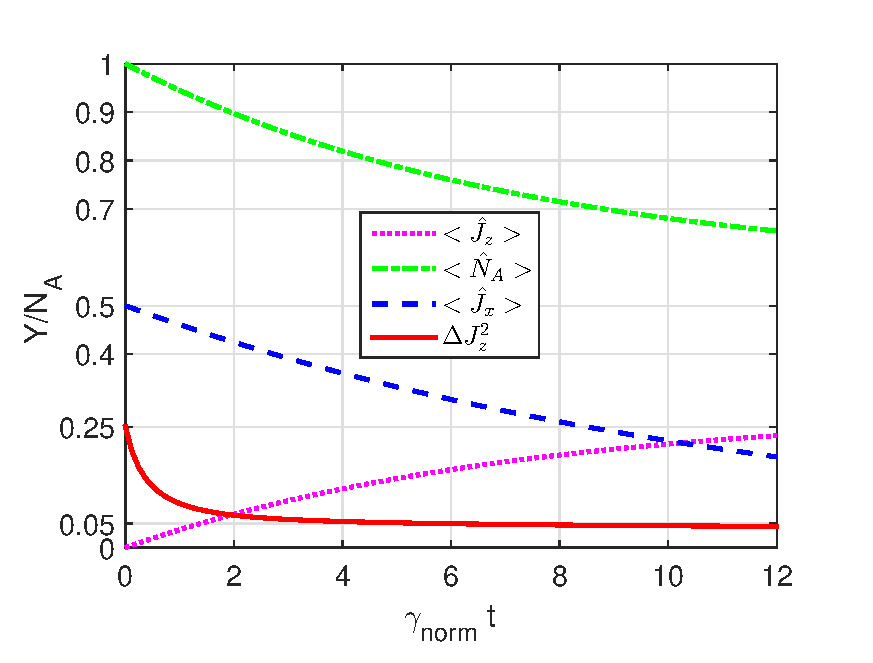
\includegraphics[scale=0.45]{../media/Figs/clockdynamics_m33_yq_rp1d5_exact}}
%\end{minipage}
%\begin{minipage}{.5\linewidth}
%\centering
%\subfloat[]{\label{fig:clockdynamics_m33_yq_rp1d5_approx}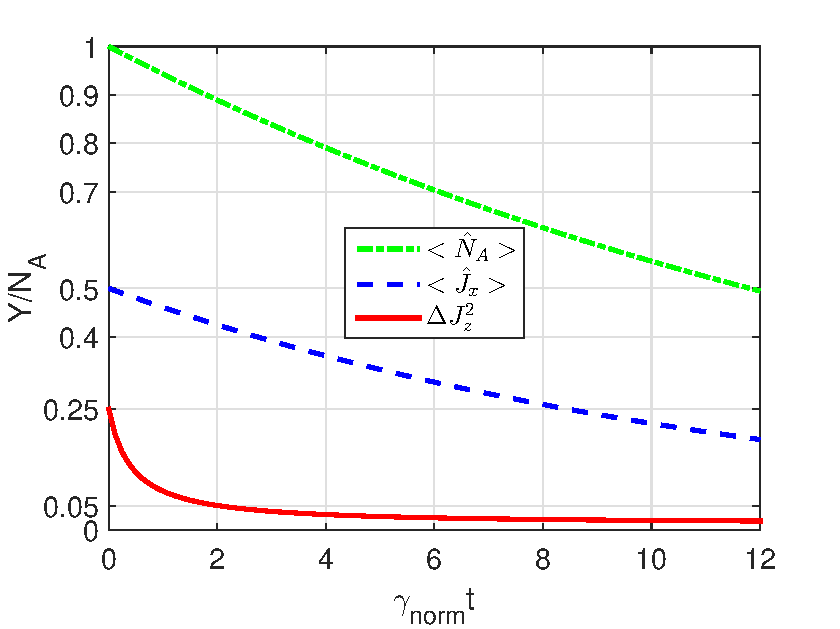
\includegraphics[scale=0.45]{../media/Figs/clockdynamics_m33_yq_rp1d5_approx}}
%\end{minipage}
%\par\medskip
%\begin{minipage}{.5\linewidth}
%\centering
%\subfloat[]{\label{fig:clockdynamics_m44_yq_rp1d5_exact}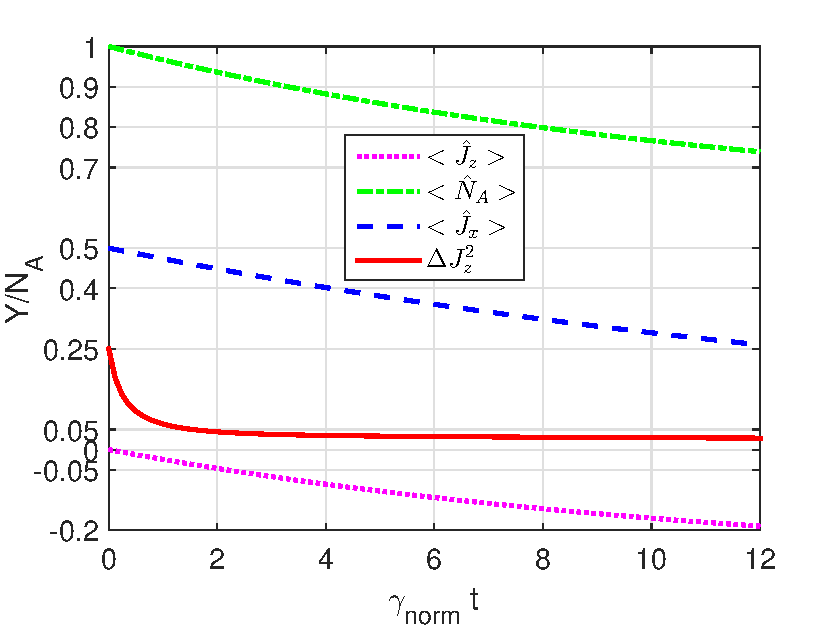
\includegraphics[scale=0.45]{../media/Figs/clockdynamics_m44_yq_rp1d5_exact}}
%\end{minipage}
%\begin{minipage}{.5\linewidth}
%\centering
%\subfloat[]{\label{fig:clockdynamics_m44_yq_rp1d5_approx}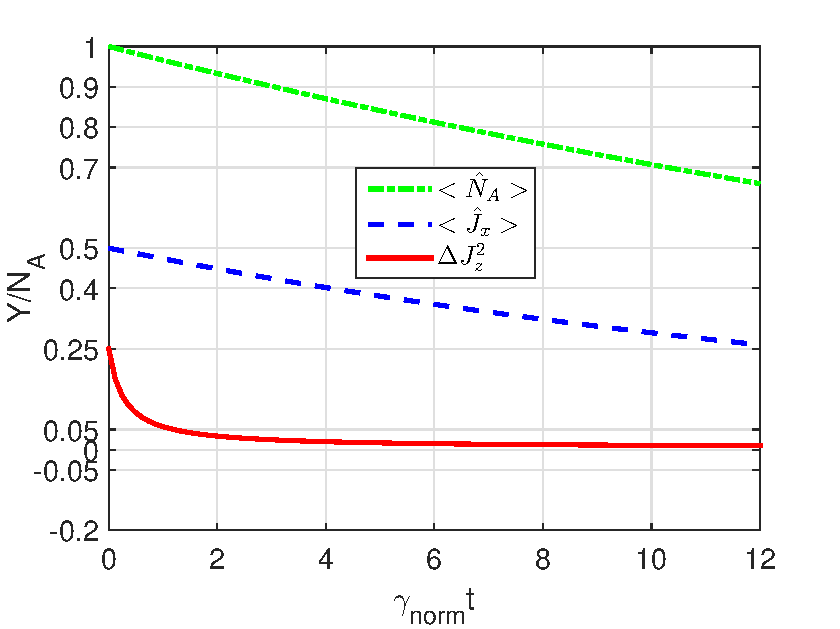
\includegraphics[scale=0.45]{../media/Figs/clockdynamics_m44_yq_rp1d5_approx}}
%\end{minipage}
%\caption{Evolution of expectation values of collective spin operators as a function of time with $ N_A=1000 $ atoms trapped at $ r'\!_\perp =1.5a $ along the $ H/x $ axis of the nanofiber. Subfigs.~\protect\subref{fig:clockdynamics_m33_yq_rp1d5_exact} and~\protect\subref{fig:clockdynamics_m33_yq_rp1d5_approx} use the magic frequencies close to the $ F=3\leftrightarrow F'=3 $ transition frequency $ \omega_{33'} $. Subfigs.~\protect\subref{fig:clockdynamics_m44_yq_rp1d5_exact} and~\protect\subref{fig:clockdynamics_m44_yq_rp1d5_approx} used the magic frequencies close to $ \omega_{44'} $. The $ \phi $ axis was defined as the quantization axis for these plots. Subfigs.~\protect\subref{fig:clockdynamics_m33_yq_rp1d5_exact} and~\protect\subref{fig:clockdynamics_m44_yq_rp1d5_exact} were calculated using the exact solution of the coupled differential equations of the expectation values of spin operators. In contrast, Subfigs.~\protect\subref{fig:clockdynamics_m33_yq_rp1d5_approx} and~\protect\subref{fig:clockdynamics_m44_yq_rp1d5_approx} use approximations by ignoring the dynamics of $ \expect{\hat{J}_z} $ for all calculations, and treat $ \expect{\hat{N}_C} $ as a constant in solving the differential equation for $ \Delta J_z^2 $. Other parameters used: $ \Omega/2\pi=52 $ MHz (does not matter). }\label{fig:clockdynamics_m_yq_rp1d5}
%\end{figure}

%\begin{figure}
%\begin{minipage}{.5\linewidth}
%\centering
%\subfloat[]{\label{fig:xi_magic33_yq}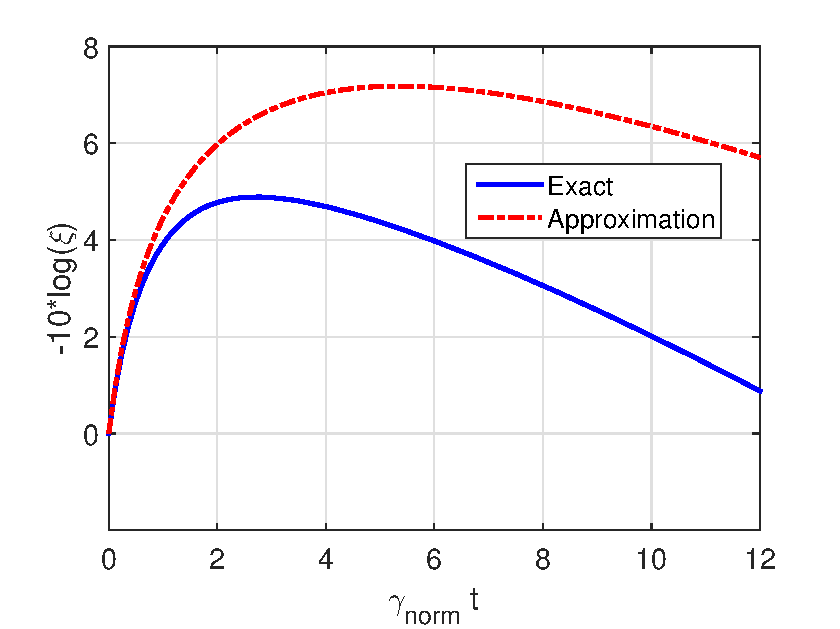
\includegraphics[scale=0.45]{../media/Figs/xi_magic33_yq}}
%\end{minipage}
%\begin{minipage}{.5\linewidth}
%\centering
%\subfloat[]{\label{fig:xi_magic44_yq}\includegraphics[scale=0.45]{../media/Figs/xi_magic44_yq}}
%\end{minipage}
%\par\medskip
%\begin{minipage}{.5\linewidth}
%\centering
%\subfloat[]{\label{fig:xi_magic33_xq}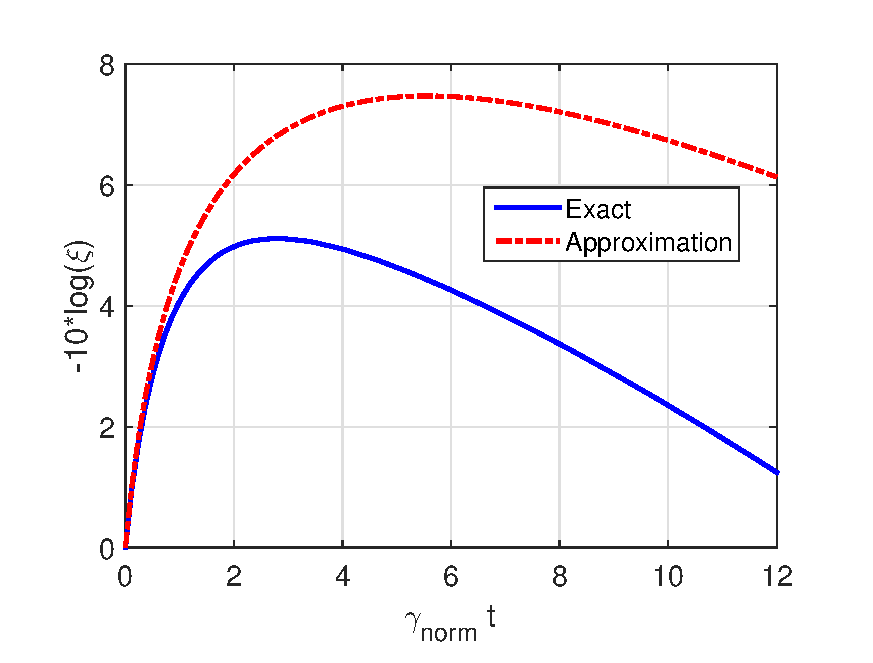
\includegraphics[scale=0.45]{../media/Figs/xi_magic33_xq}}
%\end{minipage}
%\begin{minipage}{.5\linewidth}
%\centering
%\subfloat[]{\label{fig:xi_magic44_xq}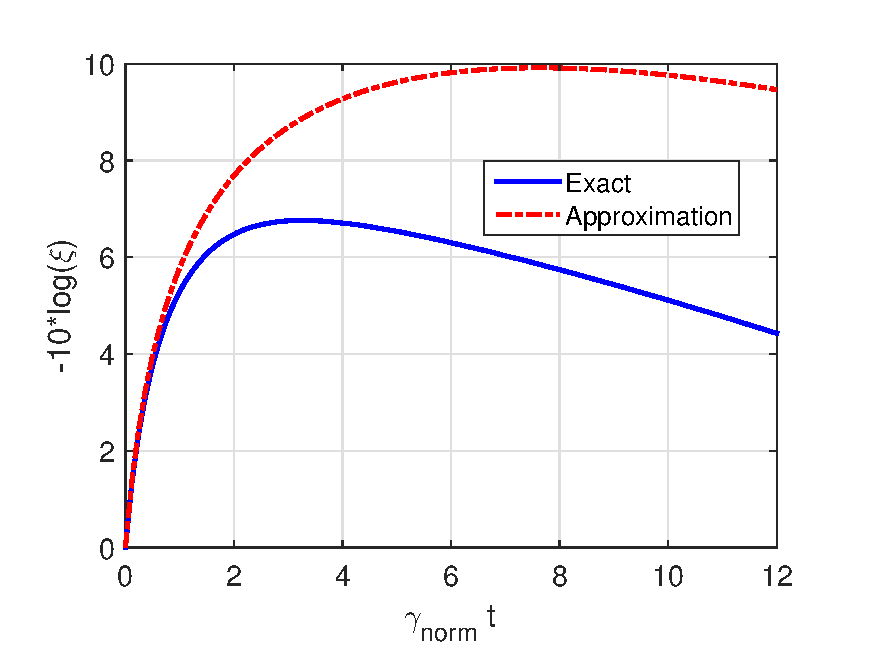
\includegraphics[scale=0.45]{../media/Figs/xi_magic44_xq}}
%\end{minipage}
%%\centering\makebox[\textwidth]{
%%\includegraphics[width=0.65\textwidth]{./Figs/xi_magic44_yq}}
%\caption{Spin squeezing evolution as a function of time with $ N_A=1000 $ atoms trapped at $ r'\!_\perp =1.5a $ along the $ H/x $ axis of the nanofiber. Subfigs.~\protect\subref{fig:xi_magic33_yq} and~\protect\subref{fig:xi_magic33_xq} use the magic frequencies close to the $ F=3\leftrightarrow F'=3 $ transition frequency $ \omega_{33'} $. Subfigs.~\protect\subref{fig:xi_magic44_yq} and~\protect\subref{fig:xi_magic44_xq} used the magic frequencies close to $ \omega_{44'} $. The magic frequencies and spin squeezing parameters are different for different choices of quantization axis. Subfigs.~\protect\subref{fig:xi_magic33_yq} and~\protect\subref{fig:xi_magic44_yq} define $ \phi $ axis as the quantization axis. In contrast, subfigs.~\protect\subref{fig:xi_magic33_xq} and~\protect\subref{fig:xi_magic44_xq} use $ r\!_\perp $ axis as the quantization axis. When $ z $ axis is chosen to be the quantization axis, almost no squeezing effect can be observed at the magic frequencies. As can be seen, when the quantization axis close to the local field direction, the spin squeezing parameter can reach to a higher value. Other parameters used: $ \Omega/2\pi=52 $ MHz (does not matter). }\label{fig:xi_magic}
%\end{figure}

%</birefringencemotioneq>

%\bibliography{Nanofiber}
%\bibliographystyle{amsplain}
\bibliographystyle{../styles/abbrv-alpha-letters-links}
%\bibliographystyle{unsrt}
% \nocite{*}
\bibliography{../refs/Archive,../chap4/Nanofiber}

\printindex

\end{document}          




%\chapter{QND measurement and spin squeezing using the Faraday effect}
%\mathversion{normal}
\ExecuteMetaData[../chap5/CooperativityEnhancement.tex]{Faradayprotocol}
%\mathversion{normal}

\chapter{Two-color scheme towards practical spin squeezing}

\chapter{Conclusion and outlook}

\appendix

\chapter{Maxwell's Equations for an waveguide}
This chapter will dedicate to some fundamental theory of Maxwell's equations. More detailed 
discussions can be found in Ref.~\cite{Snyder1983}. Some detailed solution of Maxwell's equation 
applied to cylindrical structures can be found in Ref.~\cite{Wait1959}. 

For non-magnetic materials which normally constitute an optical waveguide with $ \mu=\mu_0 $, the 
spatial dependence of the electrical field $ \boldsymbol{\mathcal{E}}(\br) $ and the magnetic field $ 
\boldsymbol{\mathcal{H}}(\br) $ of an optical waveguide is determined by Maxwell's equations:
\begin{align}
\nabla\times \boldsymbol{\mathcal{E}} &= i(\mu_0/\varepsilon_0)^{1/2} k \boldsymbol{\mathcal{H}}, & 
\nabla\times \boldsymbol{\mathcal{H}} &= \boldsymbol{\mathcal{J}}-i(\varepsilon_0/\mu_0)^{1/2}kn^2 
\boldsymbol{\mathcal{E}}, \label{EHtimesMKS}\\
\nabla\cdot (n^2 \boldsymbol{\mathcal{E}}) &= \rho/\varepsilon_0, & \nabla\cdot 
\boldsymbol{\mathcal{H}} &=0, \label{EHdotsMKS}
\end{align}
where $ \boldsymbol{\mathcal{J}} $ and $ \rho $ are the current density and charge density, $ 
\varepsilon=n^2 \varepsilon_0 $ is the dielectric constant of the waveguide as a function of space, and $ 
k=2\pi/\lambda=\omega/c $.  We usually assume an implicit chromatic time dependence factor $ \exp(-i\omega t) $ in the 
full field vectors. These equations above are written in MKS units. 

Sometimes, to avoid the dielectric constant $ \varepsilon_0 $ and magnetic permeability $ \mu_0 $ of 
free space, we can rewrite the Maxwell's equations in Gauss units, which yield
\begin{align}
\nabla \times \boldsymbol{\mathcal{E}} &= -\frac{1}{c} \pt{\boldsymbol{\mathcal{B}}}=i 
k\boldsymbol{\mathcal{B}}, & \nabla \times 
\boldsymbol{\mathcal{H}} &= \frac{4\pi}{c} \boldsymbol{\mathcal{J}} + 
\frac{1}{c}\pt{\boldsymbol{\mathcal{D}}}= \frac{4\pi}{c}\boldsymbol{\mathcal{J}} 
-ik\boldsymbol{\mathcal{D}}, \label{eq:maxwelldiv}\\
\nabla \cdot \boldsymbol{\mathcal{D}} &= 4\pi \rho, & \nabla \cdot \boldsymbol{\mathcal{B}} &=0,\label{eq:maxwellgrad}
\end{align}
where $ \boldsymbol{\mathcal{D}} = \varepsilon \boldsymbol{\mathcal{E}}=\varepsilon_r \boldsymbol{\mathcal{E}} $ and $ 
\boldsymbol{\mathcal{B}}= \mu\boldsymbol{\mathcal{H}}\approx \boldsymbol{\mathcal{H}} $ for non-magnetic materials. By default, we will use Gauss units in this piece of work, and only consider non-magnetic materials. Notice that, we make the dielectric constant equal to the relative dielectric constant ($ \varepsilon=\varepsilon $) in the Gauss units convention.  

Equations~\eqref{eq:maxwelldiv} can lead to the wave equation for a chromatic electric field in Gauss units as
\begin{align}
-\nabla \times (\nabla \times \boldsymbol{\mathcal{E}})+\varepsilon k^2\boldsymbol{\mathcal{E}}=-ik\frac{4\pi}{c} \boldsymbol{\mathcal{J}}. \label{eq:waveeqGaussU}
\end{align}
Similarly, the corresponding wave equation in SI units can be given by
\begin{align}
-\nabla \times (\nabla \times \boldsymbol{\mathcal{E}})+ n^2 k^2\boldsymbol{\mathcal{E}}=-ik\sqrt{\frac{\mu_0}{\varepsilon_0}} \boldsymbol{\mathcal{J}}.
\end{align}

We can further simplify the equation above by using 
\begin{align}
\nabla\times (\nabla\times \bmc{E}) &= -\nabla(\nabla\cdot \bmc{E})+ \nabla^2\bmc{E}. 
\end{align}
In the case that there is no net charge and current in the space, the wave equations above in both Gauss and SI units can be simplified to be
\begin{align}\label{eq:freespacewaveeq}
(\nabla^2 + n^2k^2) \boldsymbol{\mathcal{E}}=0.
\end{align}

\section{Fields of translationally invariant waveguides}
We define the axis of the waveguide is along $ z $-direction, and the refractive index profile of the 
waveguide is independent of $ z $, i.e. $ n=n(\br\!_\perp) $, which means the waveguide is 
translationally invariant. The fields of the waveguide can then be rewritten in a separable form
\begin{align}
\bmc{E}(\br) &= \bmc{E}(\br\!_\perp)\exp(i\beta z), & \bmc{H}(\br) &= \bmc{H}(\br\!_\perp)\exp(i\beta 
z),
\end{align}
where $ \beta $ is the propagation constant and $ \br\!_\perp $ is the position vector in the transverse 
plane perpendicular to the $ z $-axis. We can further decompose these fields into longitudinal and 
transverse components, parallel and orthogonal to the waveguide axis, respectively, and denoted by 
subscripts $ z $ and $ \perp $. That is
\begin{align}\label{EHtranslong}
\bmc{E}(\br) &= \left( \bmc{E}\!_\perp + \mathcal{E}_z \hat{e}_z \right)\exp(i\beta z), & \bmc{H}(\br) &= 
\left( \bmc{H}\!_\perp + \mathcal{H}_z \hat{e}_z\right) \exp(i\beta z)
\end{align}

Notice that, in literature, many authors use the sign parameter $ f=\pm 1 $ in front of $ \beta $ to indicate the propagating direction of the fields. Here, we define forward- and backward-propagating waves using the sign of the product of $ \beta z $. This is convenient to differ the contour integration paths when we decompose the radiation and guided modes for $ z=z-z'>0 $ or $ z=z-z'<0 $ cases. 

\section{Relationships between field components}\label{MWE:components}
By substituting Equ.~\ref{EHtranslong} into the source-free Maxwell equations 
(Equs.~\ref{EHtimesMKS} and~\ref{EHdotsMKS} with $ \bmc{J}=0,\, \rho=0 $), and comparing 
longitudinal and transverse components, we obtain the relationships between fields components as 
below
\begin{subequations}
\label{EHtz0}
\begin{align}
\bmc{E}\!_\perp &= -\left(\frac{\mu_0}{\varepsilon_0} \right)^{1/2} \frac{1}{kn^2} \hat{e}_z \times 
\left(\beta \bmc{H}\!_\perp + i\nabla\!_\perp \mathcal{H}_z \right),\\
\bmc{H}\!_\perp &= \left(\frac{\varepsilon_0}{\mu_0} \right)^{1/2} \frac{1}{k} \hat{e}_z \times \left(\beta 
\bmc{E}\!_\perp +i\nabla\!_\perp \mathcal{E}_z \right),\\
\mathcal{E}_z &= i\left(\frac{\mu_0}{\varepsilon_0} \right)^{1/2} \frac{1}{kn^2} \hat{e}_z \cdot 
\nabla\!_\perp \times \bmc{H}\!_\perp = \frac{i}{\beta} \left( \nabla\!_\perp \cdot \bmc{E}\!_\perp + 
(\bmc{E}\!_\perp \cdot \nabla\!_\perp) \ln n^2 \right),\\
\mathcal{H}_z &= -i \left(\frac{\varepsilon_0}{\mu_0} \right)^{1/2} \frac{1}{k}\hat{e}_z \cdot 
\nabla\!_\perp \times \bmc{E}\!_\perp = \frac{i}{\beta} \nabla\!_\perp \cdot \bmc{H}\!_\perp. 
\end{align}
\end{subequations}

Now we consider the waveguide of cylindrical fiber case. Due to symmetry, we tend to use the 
cylindrical coordinate system, which gives 
\begin{align}
\nabla\!_\perp = \hat{r}\!_\perp \pp{}{r\!_\perp} + \hat{\phi} \frac{1}{r\!_\perp} \pp{}{\phi}.
\end{align}
Therefore, Equ.~\ref{EHtz0} implies that the transverse components can be expressed in terms of the 
longitudinal components by
\begin{subequations}
\begin{align}
\mathcal{E}_{r\!_\perp} &= \frac{i}{\kappa_i^2} \left[ \beta \pp{\mathcal{E}_z }{r\!_\perp} + 
\left(\frac{\mu_0}{\varepsilon_0} \right)^{1/2}  \frac{k}{r\!_\perp} 
\pp{\mathcal{H}_z}{\phi} \right], \\
\mathcal{E}_\phi &= \frac{i}{\kappa_i^2} \left[\frac{\beta}{r\!_\perp} 
\pp{\mathcal{E}_z}{\phi} -\left(\frac{\mu_0}{\varepsilon_0} \right) ^{1/2} k 
\pp{\mathcal{H}_z}{r\!_\perp} 
\right],\\
\mathcal{H}_{r\!_\perp} &= \frac{i}{\kappa_i^2} \left[ \beta \pp{\mathcal{H}_z}{r\!_\perp} 
-\left(\frac{\varepsilon_0}{\mu_0} \right)^{1/2} \frac{kn^2}{r\!_\perp}\pp{\mathcal{E}_z}{\phi} \right],\\
\mathcal{H}_\phi &= \frac{i}{\kappa_i^2} \left[ \frac{\beta}{r\!_\perp} \pp{\mathcal{H}_z}{\phi} + 
\left(\frac{\varepsilon_0}{\mu_0} \right)^{1/2} kn^2 \pp{\mathcal{E}_z}{r\!_\perp} \right],
\end{align}
\end{subequations}
with $ \kappa_i^2= k^2n_i^2-\beta^2=k^2 \varepsilon_i -\beta^2  $ and $ n=n(\br\!_\perp)=n_i$ for corresponding region $i$. 

Correspondingly, the component relationships in Gauss units are
\begin{subequations}\label{EHzgauss}
\begin{align}
\mathcal{E}_{r\!_\perp} &= \frac{i}{\kappa_i^2} \left[ \beta \pp{\mathcal{E}_z }{r\!_\perp} + 
  \frac{k}{r\!_\perp} 
\pp{\mathcal{H}_z}{\phi} \right]= \frac{i\beta}{\kappa_i^2} \pp{\mathcal{E}_z }{r\!_\perp} - 
  \frac{km}{r\!_\perp \kappa_i^2} {\mathcal{H}_z}, \\
\mathcal{E}_\phi &= \frac{i}{\kappa_i^2} \left[\frac{\beta}{r\!_\perp} 
\pp{\mathcal{E}_z}{\phi} - k 
\pp{\mathcal{H}_z}{r\!_\perp} 
\right] = -\frac{\beta m}{r\!_\perp \kappa_i^2} 
{\mathcal{E}_z} - \frac{ik}{\kappa_i^2} 
\pp{\mathcal{H}_z}{r\!_\perp},\\
\mathcal{H}_{r\!_\perp} &= \frac{i}{\kappa_i^2} \left[ \beta \pp{\mathcal{H}_z}{r\!_\perp} 
- \frac{kn^2}{r\!_\perp}\pp{\mathcal{E}_z}{\phi} \right]= \frac{i\beta}{\kappa_i^2} \pp{\mathcal{H}_z}{r\!_\perp} 
+ \frac{kn^2m}{r\!_\perp \kappa_i^2} {\mathcal{E}_z},\\
\mathcal{H}_\phi &= \frac{i}{\kappa_i^2} \left[ \frac{\beta}{r\!_\perp} \pp{\mathcal{H}_z}{\phi} + 
 kn^2 \pp{\mathcal{E}_z}{r\!_\perp} \right] = -\frac{\beta m}{r\!_\perp \kappa_i^2} {\mathcal{H}_z} + 
  \frac{ikn^2}{\kappa_i^2} \pp{\mathcal{E}_z}{r\!_\perp}.
\end{align}
\end{subequations}


\textcolor{red}{Vector and Scalar operators in various coordinate systems...}



\chapter{Some Basic Properties of Bessel Functions}
Below, we collect some basic properties of Bessel functions without proving. Detailed properties of Bessel functions can be found in some books (see, for example, Ref.~\cite{Watson1995}).

Bessel's differential equation Bessel functions:
\begin{align}
x^2\sdd{R(x)}{x}+x\dd{R(x)}{x}+(x^2-m^2)R(x)=0,
\end{align}
where $R(x)$ is a Bessel function with index $m$. 

Recurrence relations for the first kind of Bessel functions:
\begin{align}
J_m(x)=\frac{m+1}{x}J_{m+1}(x)+\dd{J_{m+1}(x)}{x}=\frac{m-1}{x}J_{m-1}-\dd{J_{m-1}(x)}{x}.
\end{align}

Derivatives of Bessel functions:
\begin{align}
J_m^\prime(x)&=\frac{1}{2}(J_{m-1}(x)-J_{m+1}(x))\\
{H^{(1)}_m}^\prime (x) &=\frac{1}{2}({H^{(1)}_{m-1}}^\prime (x)-{H^{(1)}_{m+1}}^\prime(x))
\end{align}

\ExecuteMetaData [../chap2/WaveguideInterface.tex]{eigenmode}

\ExecuteMetaData [../chap2/WaveguideInterface.tex]{paraxialexpansion}



\ExecuteMetaData [../chap2/WaveguideInterface.tex]{nanofiberradiationproblem}

\chapter{Cylindrical function decomposition of a tilted incident plane wave}\label{Ch:PlanewaveDecomposition}
As an example of applying the mode decomposition technique we used above to find the projected bounded and unbounded modes under cylindrical boundary conditions, below, we demonstrate a simple case on decomposing a tilted incident plane wave into corresponding cylindrical modes. The solution might be useful to give us some insights on solving the corresponding nanofiber problem when an external field presents, which is the case for some cooling and state preparation protocols demonstrated in experiments~\cite{Meng2017ground,Ostfeldt2017Dipole}. 

The key to solve this kind of problems is to decompose all field functions into cylindrical functions. The bare nanofiber modes have already been decomposed into cylindrical functions in the last section; therefore, here, we only need to decompose the incident field as cylindrical functions. 

We assume the incident plane wave is given by
\begin{equation}
\mathbf{E}(\br,t)=\re\left[\mathbf{U}(\br,t) \right]=\mathbf{E}_0 \cos (\mathbf{k}\cdot\mathbf{r}-\omega t + \phi_0),
\end{equation}
where the forward propagating wave can be given by
\begin{align}
\mathbf{U}(\br,t) &= \mathbf{U}_0e^{i(\mathbf{k}\cdot\mathbf{r}-\omega t + \phi_0)}\\
&= \mathbf{U}_0e^{i\mathbf{k}\cdot\mathbf{r}}e^{i(\phi_0-\omega t )}.
\end{align}
with the initial phase, $\phi_0$, and the vector amplitude of $\mathbf{U}_0$. We can ignore the phase offset, and separate the spatial and temporal parts for the forward-propagating field. We want to expand the plane wave function into cylindrical functions, and thus we can apply the technique we used in the last appendix to solve the boundary condition problem and decompose the bound and radiation modes. The only term that needs to be expanded is the $ e^{i\mathbf{k}\cdot\mathbf{r}} $ factor. 

We define $ \mathbf{k}\cdot\mathbf{r}=(k\!_{\perp}\mathbf{e}\!_{k\!_\perp}+k_z\mathbf{e}_{z}) \cdot(r\!_{\perp}\mathbf{e}\!_{r\!_\perp}+z\mathbf{e}_{z}) = k\!_{\perp}r\!_{\perp}\cos(\phi_{k}-\phi_{r})+k_{z}{z}= k\!_\perp r\!_\perp \cos \Delta\phi +k_{z}{z}$, where $ \Delta\phi=\phi_{k}-\phi_{r} \in [0,2\pi)$ is the angle between $ \mathbf{e}_{k\!_\perp} $ and $ \mathbf{e}_{r\!_\perp} $. Thus
\begin{align}
e^{i\mathbf{k}\cdot \mathbf{r}}=e^{ik\!_\perp r\!_\perp\cos\Delta\phi}e^{ik_{z}{z}}
\end{align}
is a periodic function of $ \Delta\phi $ and hence can be expanded into a Fourier series given below. 
\begin{align}
e^{i\mathbf{k}\cdot \mathbf{r}} &= \sum_{m=-\infty}^{\infty}c_{m}(k\!_\perp r\!_\perp)e^{im\Delta\phi}e^{ik_{z}{z}},
\end{align}
where the coefficients $ c_{m}(k\!_\perp r\!_\perp) $ is associated with Bessel's first integral\index{Bessel function!Bessel's first integral}~\footnote{see Jackson's E\&M of Ref.~\cite{Jackson1975}, on page 140.}
\begin{align}
c_{m}(k\!_\perp r\!_\perp)&= \frac{1}{2\pi} \int_0^{2\pi} e^{ik\!_\perp r\!_\perp\cos \Delta\phi}e^{-im\Delta\phi}\mathrm{d}\Delta\phi\\
&=i^mJ_m(k\!_\perp r\!_\perp).
\end{align}
Therefore, we have
\begin{align}
e^{i\mathbf{k}\cdot \mathbf{r}} &=\sum_{m=-\infty}^{\infty}i^me^{im\Delta\phi}e^{ik_{z}{z}}J_m(k\!_\perp r\!_\perp).
\end{align}

Notice that the first kind of Bessel's function\index{Bessel function!Bessel function of the first kind} usually represent standing radial waves, while Hankel functions\index{Hankel function} usually describe traveling waves. Using the relationships that $ J_{m}(k\!_\perp r\!_\perp)=H_{m}^{(1)}(k\!_\perp r\!_\perp)+H_{m}^{(2)}(k\!_\perp r\!_\perp) $, we can re-express the plane wave in terms of incoming (at negative r) and outgoing (at positive r) as below.
\begin{align}
e^{i\mathbf{k}\cdot \mathbf{r}} &=\sum_{m=-\infty}^{\infty}i^me^{im\Delta\phi}e^{ik_{z}{z}} H_{m}^{(1)}(k\!_\perp r\!_\perp)+\sum_{m=-\infty}^{\infty}i^me^{im\Delta\phi}e^{ik_{z}{z}} H_{m}^{(2)}(k\!_\perp r\!_\perp).
\end{align}

This result shows that only when $ k_z=\beta $ can the tilted plane wave contributes to nanofiber modes be with wavenumber $ \beta $, since both $ k_z $ and $ \beta $ have consistent physics meaning. Therefore, when a plane wave comes perpendicular to the fiber axis, the wave can rarely couple to the fiber's guided modes, which is good for minimizing the influence of the incident external field directly mixed into the detected signal at the end of the fiber. 

\ExecuteMetaData [../chap2/WaveguideInterface.tex]{choozingSWGs}


%\chapter{Project dipole radiation onto nanofiber modes: far field approximation (a rough model)}\label{ch:FreeDipoleProjection}
As a trial, we only add one atom in the nanofiber-trapped-atoms system. 
Considering the detector is far away from the atom compared to the distance between the atom and the nanofiber, the paraxial approximation\index{paraxial approximation} holds for our case where our measurement on the optical field is applied after a distant transmission through the fiber. \textcolor{red}{We also assume that the emission from the atom propagates in free space by vanishing the boundary condition defined by the nanofiber, so that we can use the conclusion of the Green function for free space. }
The scattered optical field can be written as 
\begin{align}
\boldsymbol{\mathcal{E}}^s(\br) &=-k_0^2\left(\boldsymbol{\alpha}\cdot \boldsymbol{\mathcal{E}}^g(\br')\right)_\perp \frac{e^{ik_0 \left| \br-\br' \right| }}{\left| \br-\br'\right| }\\
&=-k_0^2\left[ \boldsymbol{\alpha}\!\cdot\! \boldsymbol{\mathcal{E}}^g(\br') - \left(\hat{\mathrm{r}}\! \cdot\! \boldsymbol{\alpha}\!\cdot\! \boldsymbol{\mathcal{E}}^g(\br') \right) \hat{\mathrm{r}}\right] \frac{e^{ik_0 \left| \br-\br' \right| }}{\left| \br-\br'\right| }\\
&\approx -k_0^2\left[ \boldsymbol{\alpha}\!\cdot\! \boldsymbol{\mathcal{E}}^g(\br') - \left(\hat{\mathrm{e}}_z\! \cdot\! \boldsymbol{\alpha}\!\cdot\! \boldsymbol{\mathcal{E}}^g(\br') \right) \hat{\mathrm{e}}_z\right] \frac{e^{ik_0 \left| \br-\br' \right| }}{\left| \br-\br'\right| }\\
&=-k_0^2 \left[\left(\hat{\mathrm{e}}_{r_\perp} \! \cdot \! \boldsymbol{\alpha} \! \cdot\! \boldsymbol{\mathcal{E}}^g(\br')\right)\hat{\mathrm{e}}_{r_\perp} + \left(\hat{\mathrm{e}}_\phi \! \cdot \! \boldsymbol{\alpha} \! \cdot \! \boldsymbol{\mathcal{E}}^g(\br') \right)\hat{\mathrm{e}}_\phi \right] 
\frac{e^{ik_0 \left| \br-\br' \right| }}{\left| \br-\br'\right| }\\
&\approx \frac{-k_0^2 e^{ik_0(z\!-\!z'\!)}}{z\!-\!z'}\left[\left(\hat{\mathrm{e}}_{r_\perp} \!\!\cdot\! \boldsymbol{\alpha}\!\cdot\! \boldsymbol{\mathcal{E}}^g(\br')\right)\hat{\mathrm{e}}_{r_\perp} \!\! +\! \left(\hat{\mathrm{e}}_\phi\!\cdot\! \boldsymbol{\alpha}\!\cdot\! \boldsymbol{\mathcal{E}}^g(\br') \right)\hat{\mathrm{e}}_\phi \right] \exp\!\! \left[ \frac{ik_0 \left| \mathrm{r}_\perp\! - \mathrm{r}_\perp'\right|}{2(z-z')}  \right],\label{Erscatt}
\end{align}
where $ \boldsymbol{\alpha} $ is the polarizability tensor only depending on the internal state of the atom; $ \left| \mathrm{r}_\perp - \mathrm{r}_\perp'\right|=\sqrt{r_\perp^2+{r_\perp'}^2 - 2 r_\perp r_\perp'\cos(\phi-\phi')} $ where $ (r_\perp',\phi',z') $ is the coordinate of the atom. 

As shown in Equ.~\ref{Erscatt}, the scattered field does not have a $ z $-component in the far field by using a free space Green function. 

We can decompose the guided mode into left- and right-handed circular fundamental modes using Equ.~\ref{Eilincyc}. For instance, if the incident light is $ x $-polarized (horizontally polarized) with the normalized field $ \boldsymbol{\mathcal{E}}^g (\br)=\boldsymbol{\mathcal{E}}_H (\br) $, and $ \mathbf{E}^g (\br,t) = \boldsymbol{\mathcal{E}}_H(\br)e^{-i\omega t} $ is a forward propagating light, we can use the relationship that
\begin{subequations}
\label{ErPMHV}
\begin{align}
\boldsymbol{\mathcal{E}}^+ &= \frac{1}{\sqrt{2}} \left(\boldsymbol{\mathcal{E}}_H+i\boldsymbol{\mathcal{E}}_V \right),\\
\boldsymbol{\mathcal{E}}^- &= \frac{1}{\sqrt{2}} \left( \boldsymbol{\mathcal{E}}_H-i\boldsymbol{\mathcal{E}}_V \right),
\end{align}
\end{subequations}
where $ \boldsymbol{\mathcal{E}}_V $ is the normalized mode with a $ y $-polarized (vertically polarized) incident light which is orthogonal to $ \boldsymbol{\mathcal{E}}_H $. Based on Equ.~\ref{ErPMHV}, we can solve for $ \boldsymbol{\mathcal{E}}_H $ to give
\begin{align}
\boldsymbol{\mathcal{E}}_H &= \frac{1}{\sqrt{2}} \left(\boldsymbol{\mathcal{E}}^+ + \boldsymbol{\mathcal{E}}^- \right),\\
\boldsymbol{\mathcal{E}}_V &= \frac{i}{\sqrt{2}} \left( \boldsymbol{\mathcal{E}}^- -\boldsymbol{\mathcal{E}}^+ \right). 
\end{align}
Therefore, the spatial dependent scattered electrical field can be given by
\begin{align}
\boldsymbol{\mathcal{E}}^s(\br) &\approx  \frac{-\!k_0^2 e^{ik_0(z\!-\!z'\!)}}{z\!-\!z'}\! \left[\left(\hat{\mathrm{e}}_{r_\perp} \!\!\cdot\! \boldsymbol{\alpha}\!\cdot\! \boldsymbol{\mathcal{E}}_H(\br')\right)\hat{\mathrm{e}}_{r_\perp} \!\!  +\! \left(\hat{\mathrm{e}}_\phi\!\cdot\! \boldsymbol{\alpha}\!\cdot\! \boldsymbol{\mathcal{E}}_H(\br') \right)\hat{\mathrm{e}}_\phi \right] \exp\!\! \left[ \frac{ik_0 \left| \mathrm{r}_\perp\!\! -\! \mathrm{r}_\perp'\right|}{2(z-z')}  \right]\\
&= - \frac{k_0^2 e^{ik_0(z\!-\!z'\!)}}{\sqrt{2}(z\!-\!z')} \left(\hat{\mathrm{e}}_{r_\perp} \!\!\cdot\! \boldsymbol{\alpha}\!\cdot\! \left(\boldsymbol{\mathcal{E}}^+ (\br') \!\! +\! \boldsymbol{\mathcal{E}}^- (\br') \right)\right)\hat{\mathrm{e}}_{r_\perp}  \exp\!\! \left[ \frac{ik_0 \left| \mathrm{r}_\perp\!\! -\! \mathrm{r}_\perp'\right|}{2(z-z')}  \right] \nonumber\\
&\qquad - \frac{k_0^2 e^{ik_0(z\!-\!z'\!)}}{\sqrt{2}(z\!-\!z')} \left(\hat{\mathrm{e}}_{\phi} \!\!\cdot\! \boldsymbol{\alpha}\!\cdot\! \left(\boldsymbol{\mathcal{E}}^+ (\br') \!\! +\! \boldsymbol{\mathcal{E}}^- (\br') \right)\right)\hat{\mathrm{e}}_{\phi}  \exp\!\! \left[ \frac{ik_0 \left| \mathrm{r}_\perp\!\! -\! \mathrm{r}_\perp'\right|}{2(z-z')}  \right]. \label{Ers0}
\end{align}
Using Equs.~\ref{Ertcrla} and~\ref{Ertcrga}, the $ \boldsymbol{\mathcal{E}}_H (\br')= \boldsymbol{\mathcal{E}}^+ (\br') \!\! +\! \boldsymbol{\mathcal{E}}^- (\br') $ is given by
\begin{subequations}
\label{EHrcrla}
\begin{align}
{\mathcal{E}_H}_{r_\perp} (\br') &= A\frac{\beta_{11}}{h_{11}}\nonumber\\
&\qquad \left[ (1\!-\!s_{11})J_0(h_{11}r'_\perp)\!-\! (1\!+\!s_{11})J_2(h_{11}r_\perp') \right]e^{if\beta_{11} z'}\cos{\phi'}\\
{\mathcal{E}_H}_\phi(\br') &=  iA \frac{\beta_{11}}{2h_{11}} \nonumber\\
&\qquad \left[ (1\!-\!s_{11})J_0(h_{11}r'_\perp)\! +\! (1\!+\!s_{11})J_2(h_{11}r'_\perp) \right] e^{if\beta_{11} z' }\sin(\phi')\\
{\mathcal{E}_H}_z(\br') &= i2A J_1(h_{11}r'_\perp) e^{if\beta_{11} z'}\cos(\phi')
\end{align}
\end{subequations}
for $ r'_\perp<a $, and by
\begin{subequations}
\label{EHrpcrga}
\begin{align}
{\mathcal{E}_H}_{r_\perp}(\br') &=A\frac{\beta_{11}}{h_{11}}\frac{J_1(h_{11}a)}{K_1(q_{11}a)}\nonumber\\ 
&\qquad \left[ (1\!-\!s_{11})K_0(q_{11}r'_\perp)\!+\!(1 \!+\! s_{11})K_2(q_{11}r'_\perp) \right]e^{if\beta_{11} z' }\cos(\phi')\\
{\mathcal{E}_H}_\phi(\br') &=  iA \frac{\beta_{11}}{h_{11}} \frac{J_1(h_{11}a)}{K_1(q_{11}a)}\nonumber\\ 
&\qquad \left[ (1\!-\!s_{11})K_0(q_{11}r'_\perp) \! -\! (1\!+\!s_{11})K_2(q_{11}r'_\perp) \right] e^{if\beta_{11} z'}\sin(\phi')\\
{\mathcal{E}_H}_z(\br') &= i2A \frac{J_1(h_{11}a)}{K_1(q_{11}a)} K_1(q_{11}r'_\perp) e^{if\beta_{11} z'}\cos(\phi')
\end{align}
\end{subequations}
for $ r'_\perp>a $. We define $ \mathbf{T}^{f}(\br')= \boldsymbol{\alpha}\!\cdot \boldsymbol{\mathcal{E}}_H (\br') = \boldsymbol{\alpha}\!\cdot\! \left(\boldsymbol{\mathcal{E}}^+ (\br') \!\! +\! \boldsymbol{\mathcal{E}}^- (\br') \right) $, which is a constant vector, and only the $ r_\perp $ and $ \phi $ components contribute to the scattered field in the far field. Now, Equ.~\ref{Ers0} can be rewritten as
\begin{align}
\boldsymbol{\mathcal{E}}^s(\br) &=- \frac{k_0^2 e^{ik_0(z\!-\!z'\!)}}{\sqrt{2}(z\!-\!z')} \exp\!\! \left[ \frac{ik_0 \left| \mathrm{r}_\perp\!\! -\! \mathrm{r}_\perp'\right|}{2(z-z')}  \right]\! \left[ T_{r_\perp}^f(\br') \hat{\mathrm{e}}_{r_\perp} \! + T^f_\phi (\br') \hat{\mathrm{e}}_{\phi} \right],
\end{align}
where $ T^f_{r_\perp}(\br') $ and $ T^f_\phi (\br') $ are the $ r_\perp $ and $ \phi $ components of $ \mathbf{T}^f(\br')$. 

The total electrical field can be written as 
\begin{align}
\boldsymbol{\mathcal{E}}(\br) &= \boldsymbol{\mathcal{E}}^g(\br) + \boldsymbol{\mathcal{E}}^s(\br)\\
&\approx  \frac{1}{\sqrt{2}} \left(\boldsymbol{\mathcal{E}}^+(\br)\!\! +\! \boldsymbol{\mathcal{E}}^-(\br) \right) \nonumber\\
&\qquad - \frac{k_0^2 e^{ik_0(z\!-\!z'\!)}}{\sqrt{2}(z\!-\!z')} \left(\hat{\mathrm{e}}_{r_\perp} \!\!\cdot\! \boldsymbol{\alpha}\!\cdot\! \left(\boldsymbol{\mathcal{E}}^+ (\br') \!\! +\! \boldsymbol{\mathcal{E}}^- (\br') \right)\right)\hat{\mathrm{e}}_{r_\perp}  \exp\!\! \left[ \frac{ik_0 \left| \mathrm{r}_\perp\!\! -\! \mathrm{r}_\perp'\right|}{2(z-z')}  \right] \nonumber\\
&\qquad - \frac{k_0^2 e^{ik_0(z\!-\!z'\!)}}{\sqrt{2}(z\!-\!z')} \left(\hat{\mathrm{e}}_{\phi} \!\!\cdot\! \boldsymbol{\alpha}\!\cdot\! \left(\boldsymbol{\mathcal{E}}^+ (\br') \! +\! \boldsymbol{\mathcal{E}}^- (\br') \right)\right)\hat{\mathrm{e}}_{\phi}  \exp\!\! \left[ \frac{ik_0 \left| \mathrm{r}_\perp\!\! -\! \mathrm{r}_\perp'\right|}{2(z-z')}  \right]\\
&= \frac{1}{\sqrt{2}} \boldsymbol{\mathcal{E}}_H(\br)  \!-\! \frac{k_0^2 e^{ik_0(z\!-\!z'\!)}}{\sqrt{2}(z\!-\!z')} \exp\!\! \left[ \frac{ik_0\! \left| \mathrm{r}_\perp\!\! -\! \mathrm{r}_\perp'\right|}{2(z-z')}  \right]\!\! \left[ T^f_{r_\perp}(\br') \hat{\mathrm{e}}_{r_\perp} \!\! +\! T^f_\phi (\br') \hat{\mathrm{e}}_{\phi} \right].
\end{align}
%where $ \eye $ is the unitary diagonal tensor. Now, we can see that the total optical field strongly depends on the bound field and the polarization of the atom.

To further discuss how backward and forward scattering contribute to the bound mode, we consider both the space- and time-dependent electrical field of the scattered contribution $ \mathbf{E}^s(\br,t) $, and project it to the normalized forwarded and backwarded bound modes.  In principle, we can decompose the scattered electrical field as 
\begin{align}
\mathbf{E}^s(\br,t) =\sum_\mu C^{(\mu)}(z) \mathbf{E}^{(\mu)} (\br,t),
\end{align}
with
\begin{align}
C^{(\mu)} (z) = \int_0^{2\pi}\mathrm{d}\phi \int_0^\infty {\mathbf{E}^{(\mu)}}^* (\br,t) \cdot \mathbf{E}^s(\br,t)r_\perp \mathrm{d}r_\perp.
\end{align}

For the Green function we used above, the coefficients in the far field can be calculated as
\begin{align}
C^{(\mu)} (z) &= - \frac{k_0^2 T^{f'}_{r_\perp}(\br') e^{ik_0(z\!-\!z'\!)}}{\sqrt{2}(z\!-\!z')}\int_0^{2\pi}\mathrm{d}\phi \int_0^\infty {\mathcal{E}^{(\mu)}_{r_\perp}}^* (\br) \exp\!\! \left[ \frac{ik_0 \left| \mathrm{r}_\perp\!\! -\! \mathrm{r}_\perp'\right|}{2(z-z')}  \right]\!  r_\perp \mathrm{d}r_\perp \nonumber\\
&\quad - \frac{k_0^2 T^{f'}_\phi(\br') e^{ik_0(z\!-\!z'\!)} }{\sqrt{2}(z\!-\!z')}\int_0^{2\pi}\mathrm{d}\phi \int_0^\infty {\mathcal{E}^{(\mu)}_\phi}^* (\br) \exp\!\! \left[ \frac{ik_0 \left| \mathrm{r}_\perp\!\! -\! \mathrm{r}_\perp'\right|}{2(z-z')}  \right]\!  r_\perp \mathrm{d}r_\perp \\
&=  - \frac{k_0^2 T^{f'}_{r_\perp}(\br') e^{ik_0(z\!-\!z'\!)}}{\sqrt{2}(z\!-\!z')}\int_0^{2\pi}\mathrm{d}\phi \int_0^a {\mathcal{E}^{(\mu)}_{r_\perp}}^* (\br) \exp\!\! \left[ \frac{ik_0 \left| \mathrm{r}_\perp\!\! -\! \mathrm{r}_\perp'\right|}{2(z-z')}  \right]\!  r_\perp \mathrm{d}r_\perp \nonumber\\
&\quad - \frac{k_0^2 T^{f'}_{r_\perp}(\br') e^{ik_0(z\!-\!z'\!)}}{\sqrt{2}(z\!-\!z')}\int_0^{2\pi}\mathrm{d}\phi \int_a^\infty {\mathcal{E}^{(\mu)}_{r_\perp}}^* (\br) \exp\!\! \left[ \frac{ik_0 \left| \mathrm{r}_\perp\!\! -\! \mathrm{r}_\perp'\right|}{2(z-z')}  \right]\!  r_\perp \mathrm{d}r_\perp \nonumber\\
&\quad - \frac{k_0^2 T^{f'}_\phi(\br') e^{ik_0(z\!-\!z'\!)}}{\sqrt{2}(z\!-\!z')}\int_0^{2\pi}\mathrm{d}\phi \int_0^a {\mathcal{E}^{(\mu)}_\phi}^* (\br) \exp\!\! \left[ \frac{ik_0 \left| \mathrm{r}_\perp\!\! -\! \mathrm{r}_\perp'\right|}{2(z-z')}  \right]\!  r_\perp \mathrm{d}r_\perp \nonumber\\
&\quad - \frac{k_0^2 T^{f'}_\phi(\br') e^{ik_0(z\!-\!z'\!)}}{\sqrt{2}(z\!-\!z')}\int_0^{2\pi}\mathrm{d}\phi \int_a^\infty {\mathcal{E}^{(\mu)}_\phi}^* (\br) \exp\!\! \left[ \frac{ik_0 \left| \mathrm{r}_\perp\!\! -\! \mathrm{r}_\perp'\right|}{2(z-z')}  \right]\!  r_\perp \mathrm{d}r_\perp \\
&= - \frac{k_0^2 T^{f'}_{r_\perp}(\br') e^{ik_0(z\!-\!z'\!)\!-\!if\beta_{11} z}}{\sqrt{2}(z\!-\!z')}  \!\!\! \int_0^{2\pi}\!\!\! \mathrm{d}\phi \!\!\! \int_0^a   \mathcal{E}^{(\mu)}_{r_\perp}(r_\perp) e^{-i p\phi} 
\exp\!\! \left[ \frac{ik_0 \left| \mathrm{r}_\perp\!\! -\! \mathrm{r}_\perp'\right|}{2(z-z')}  \right]\!  r_\perp \mathrm{d}r_\perp \nonumber\\
&\quad - \frac{k_0^2 T^{f'}_{r_\perp}(\br') e^{ik_0(z\!-\!z'\!)\!-\!if\beta_{11} z}}{\sqrt{2}(z\!-\!z')}  \!\!\! \int_0^{2\pi}\!\!\! \mathrm{d}\phi \!\!\! \int_a^\infty \!\!\! {\mathcal{E}^{(\mu)}_{r_\perp}} (r_\perp) e^{-i p\phi} \exp\!\! \left[ \frac{ik_0 \left| \mathrm{r}_\perp\!\! -\! \mathrm{r}_\perp'\right|}{2(z-z')}  \right]\!  r_\perp \mathrm{d}r_\perp \nonumber\\
&\quad - \frac{k_0^2 T^{f'}_\phi(\br') e^{ik_0(z\!-\!z'\!)\!-\!if\beta_{11} z}}{\sqrt{2}(z\!-\!z')} \!\!\! \int_0^{2\pi}\!\!\! \mathrm{d}\phi \!\!\! \int_0^a \!\!\! {\mathcal{E}^{(\mu)}_\phi} (r_\perp) e^{-i p\phi} \exp\!\! \left[ \frac{ik_0 \left| \mathrm{r}_\perp\!\! -\! \mathrm{r}_\perp'\right|}{2(z-z')}  \right]\!  r_\perp \mathrm{d}r_\perp \nonumber\\
&\quad - \frac{k_0^2 T^{f'}_\phi(\br') e^{ik_0(z\!-\!z'\!)\!-\!if\beta_{11} z}}{\sqrt{2}(z\!-\!z')}  \!\!\! \int_0^{2\pi}\!\!\!\mathrm{d}\phi\!\!\!  \int_a^\infty \!\!\! {\mathcal{E}^{(\mu)}_\phi} (r_\perp) e^{-i p\phi} \exp\!\! \left[ \frac{ik_0 \left| \mathrm{r}_\perp\!\! -\! \mathrm{r}_\perp'\right|}{2(z-z')}  \right]\!  r_\perp \mathrm{d}r_\perp \\
&=  - \frac{k_0^2 T^{f'}_{r_\perp}(\br') e^{ik_0(z\!-\!z'\!)\!-\!if\beta_{11} z}}{\sqrt{2}(z\!-\!z')} \!\! \int_0^{2\pi}\!\!\! \mathrm{d}\phi \!\! \int_0^a  \!\! \mathcal{E}^{(\mu)}_{r_\perp}(r_\perp)  
\exp\!\! \left[ \frac{ik_0 \left| \mathrm{r}_\perp\!\! -\! \mathrm{r}_\perp'\right|}{2(z-z')} \!-\! i p\phi  \right]\!  r_\perp \mathrm{d}r_\perp \nonumber\\
&\quad - \frac{k_0^2 T^{f'}_{r_\perp}(\br') e^{ik_0(z\!-\!z'\!)\!-\!if\beta_{11} z}}{\sqrt{2}(z\!-\!z')}  \!\!\! \int_0^{2\pi}\!\!\!\mathrm{d}\phi \!\!\! \int_a^\infty \!\!\! {\mathcal{E}^{(\mu)}_{r_\perp}} (r_\perp)  \exp\!\! \left[ \frac{ik_0 \left| \mathrm{r}_\perp\!\! -\! \mathrm{r}_\perp'\right|}{2(z-z')} \!-\! i p\phi \right]\!  r_\perp \mathrm{d}r_\perp \nonumber\\
&\quad - \frac{k_0^2 T^{f'}_\phi(\br') e^{ik_0(z\!-\!z'\!)\!-\!if\beta_{11} z}}{\sqrt{2}(z\!-\!z')} \!\!\! \int_0^{2\pi} \!\!\! \mathrm{d}\phi \!\!\! \int_0^a\!\!\! {\mathcal{E}^{(\mu)}_\phi} (r_\perp) \exp\!\! \left[ \frac{ik_0 \left| \mathrm{r}_\perp\!\! -\! \mathrm{r}_\perp'\right|}{2(z-z')} \!-\! i p\phi \right]\!  r_\perp \mathrm{d}r_\perp \nonumber\\
&\quad - \frac{k_0^2 T^{f'}_\phi(\br') e^{ik_0(z\!-\!z'\!)\!-\!if\beta_{11} z}}{\sqrt{2}(z\!-\!z')}  \!\!\! \int_0^{2\pi}\!\!\! \mathrm{d}\phi \!\!\! \int_a^\infty \!\!\! {\mathcal{E}^{(\mu)}_\phi} (r_\perp) \exp\!\! \left[ \frac{ik_0 \left| \mathrm{r}_\perp\!\! -\! \mathrm{r}_\perp'\right|}{2(z-z')} \!-\! i p\phi \right]\!  r_\perp \mathrm{d}r_\perp. \label{Cmu1}
\end{align}
Using the relationship that $ \left| \mathrm{r}_\perp - \mathrm{r}_\perp'\right|=\sqrt{r_\perp^2+{r_\perp'}\!\!^2 - 2 r_\perp r_\perp'\cos(\phi-\phi')} $, the integral over $ \phi $ can be separated as 
\begin{align}
C^{(\mu)}_0(r_\perp,z) &= \int_0^{2\pi} \!\!\! \mathrm{d}\phi  \exp\!\! \left[ \frac{ik_0 \left| \mathrm{r}_\perp\!\! -\! \mathrm{r}_\perp'\right|}{2(z-z')} \!-\! i p\phi \right]\\
&= \int_0^{2\pi} \!\!\! \mathrm{d}\phi  \exp\!\! \left[ \frac{ik_0 \sqrt{r_\perp^2+{r_\perp'}\!\!^2 - 2 r_\perp r_\perp'\cos(\phi-\phi')} }{2(z-z')} \!-\! i p\phi \right]\\
&= \int_0^{2\pi} \!\!\! \mathrm{d}\phi  \exp\!\! \left[ \frac{ik_0 \sqrt{r_\perp^2 \!+ {r_\perp'}\!\!^2}\sqrt{1 \!-\! \frac{2 r_\perp r_\perp'}{r_\perp^2 \!+ {r_\perp'}\!\!^2}\cos(\phi \!-\! \phi')} }{2(z-z')} \!-\! i p\phi \right].
\end{align}
Calculating this integration analytically is not trivial unless $ r_\perp=r_\perp' $ or $ \br_\perp $ parallel to $ \br_\perp' $. We can calculate the projection coefficients numerically instead. Equ.~\ref{Cmu1} can be rewritten as
\begin{align}
C^{(\mu)} (z) &= - \frac{k_0^2 e^{ik_0(z\!-\!z'\!)\!-\!if\beta_{11} z} }{\sqrt{2}(z\!-\!z')}\left[  T^{f'}_{r_\perp}(\br') \mathcal{C}_{r_\perp}^p (z) +  T^{f'}_\phi(\br') \mathcal{C}_{\phi}^p(z) \right]\\
&= T^{f'}_{r_\perp}(\br') \mathcal{S}_{r_\perp}^p (z) +  T^{f'}_\phi(\br') \mathcal{S}_{\phi}^p(z),
\end{align}
where $ \mathcal{C}_{r_\perp}^p(z) $ and $ \mathcal{C}_\phi^p(z) $ correspond to the integrals with $ \mathcal{E}^{(\mu)}_{r_\perp} $ and $ \mathcal{E}^{(\mu)}_{\phi} $, repectively; Correspondingly, $ \mathcal{S}_{r_\perp}^p(z)=\mathcal{A}(z)\mathcal{C}_{r_\perp}^p(z) $ and $ \mathcal{S}_{\phi}^p(z)=\mathcal{A}(z)\mathcal{C}_\phi^p(z) $, where the interference factor
\begin{align}
\mathcal{A}(z) &= - \frac{k_0^2  e^{ik_0(z\!-\!z'\!)\!-\!if\beta_{11} z}}{\sqrt{2}(z\!-\!z')}.
\end{align} 

We made $ \br'=(r'_\perp,\phi',z')=(2a,0,0) $ and $ \lambda_0=937.1 $ nm, and numerically calculated the projection coefficients for the forward propagating and counterclockwise polarized fundamental mode. The results are shown in Figs~\ref{Cz} and~\ref{ACSz}. Notice that, due to numerical inaccuracy, there are some divergent integration noises for $ z<5 $ cm. As we can see from the figures, $ \mathcal{A}(z) $ is a result of the interference of the point-scattered light and the bound mode, which decays as a function of $ \frac{1}{z-z'} $ with a periodical phase change. The phase change should have a period of $ 2\pi/(k_0-\beta_{11})\sim \lambda_0 $, where $ \beta_{11} $ is about one tenth of $ k_0 $. Due to limited computing resolution, the plots in Fig.~\ref{ACSz} does not reflect the correct phase changing period. $ \mathcal{C}^{(\mu)}(z) $ reflects how the scattered light synchronizes and better coupled with the bound mode as $ z $ increases. Combining these factors, the total projection factor $ \mathcal{S}^{(\mu)}(z) $ decays dramatically when $ z $ is small as the $ \frac{1}{z-z'} $ propagating decay dominates, and then increases with a periodical-like oscillation as the scattered light is close to a plane wave and can be well coupled and interfered with the bound mode. The beating frequency increases as the light propagates until it can be well coupled with the bound mode. Both $ r_\perp $ and $ \phi $ components of the projection coefficients have some difference as $ z $ is large. 

\textcolor{red}{Here are some phenomena needed to further explain}: the different periods of changes for $ r_\perp< a $ and $ r_\perp>a $ cases; interference periods and beating periods are not as simple as normal interference model predicted (see Fig.~\ref{../media/Figs/InterferencePeriods})--this is because we used a rough resolution in $ z $-direction to save computing time; the different behaviors of the two transverse components of the projection coefficients...

\textcolor{red}{Technical problem: numerical integration does not work well for high oscillating functions. We need to artificially set up a very fine integrating $ x $-axis to make it work properly. To fully solve this problem, we may need to consider better integration method, such as chebfun developed by Oxford (\url{http://www2.maths.ox.ac.uk/chebfun/}) which, I believe, is powerful to solve problems including definite integration, ordinary differential equations, contour integrals and roots finding. }

%\scalefig{Figs/Cr1}{0.5}{$ \mathcal{C}_{r_\perp} $ for $ r_\perp < a $ as a function of $ z $.}
\begin{figure}[H] 
\begin{minipage}{.5\linewidth}
\centering
\subfloat[$ \mathcal{C}_{r_\perp}(z) $ for $ r_\perp < a $]{\label{Cza}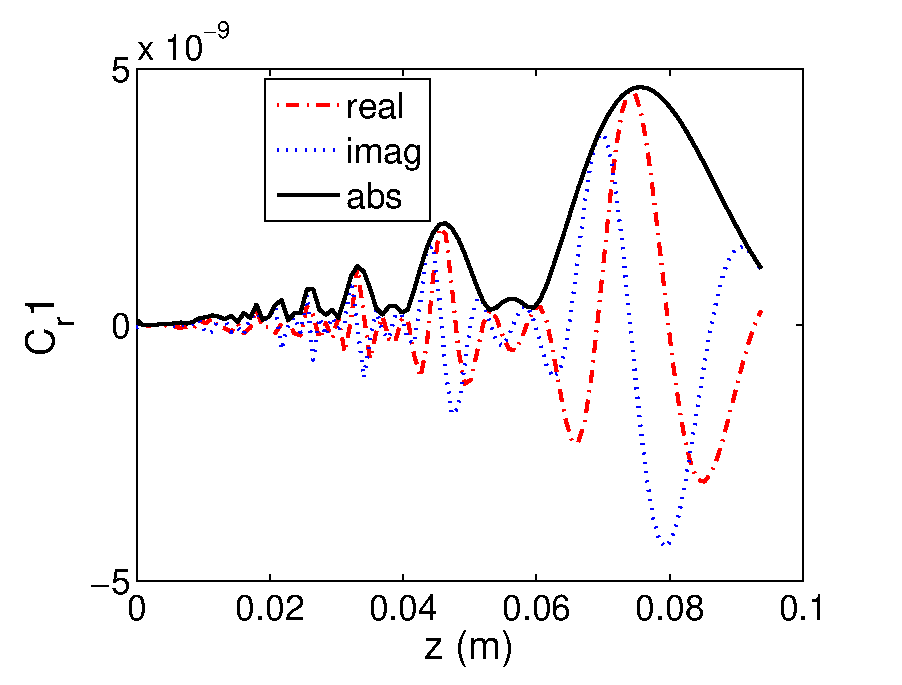
\includegraphics[scale=.44]{../media/Figs/Cr1}}
\end{minipage}%
\begin{minipage}{.5\linewidth}
\centering
\subfloat[$ \mathcal{C}_{r_\perp}(z) $ for $ r_\perp > a $]{\label{Czb}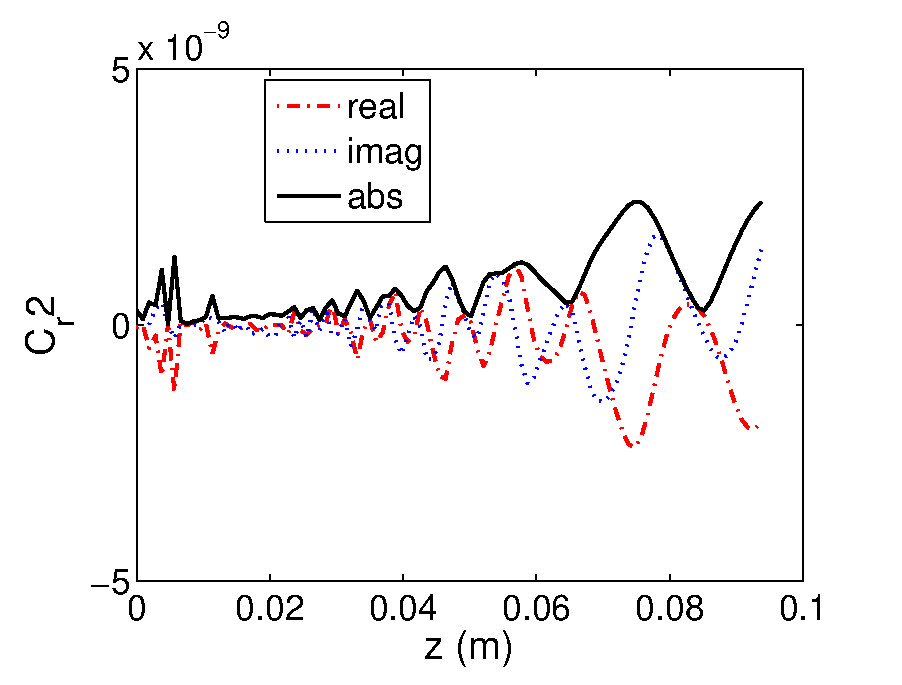
\includegraphics[scale=.44]{../media/Figs/Cr2}}
\end{minipage}
\par\medskip
\begin{minipage}{.5\linewidth}
\centering
\subfloat[$ \mathcal{C}_\phi(z) $ for $ r_\perp < a $]{\label{Czc}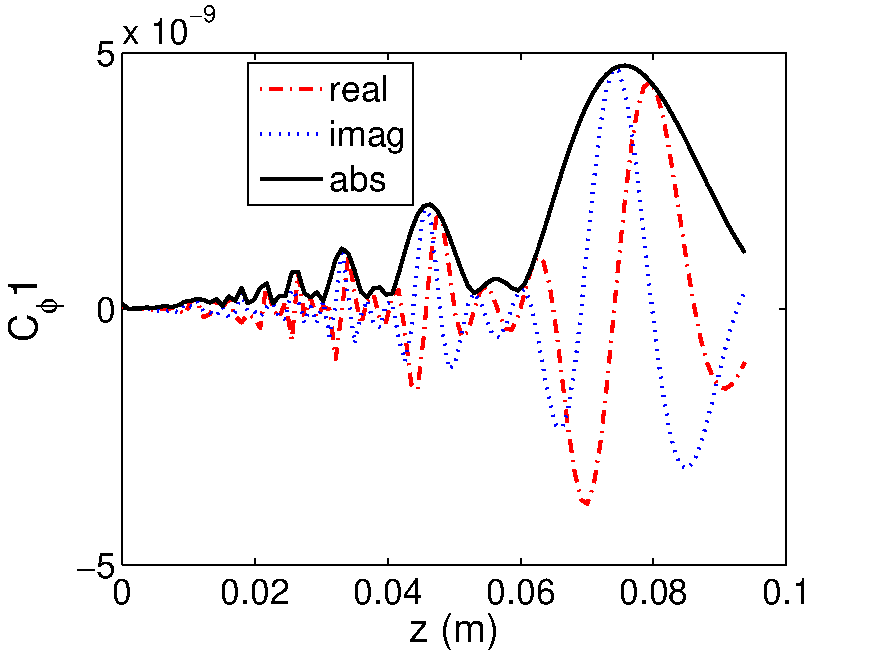
\includegraphics[scale=.44]{../media/Figs/Cphi1}}
\end{minipage}%
\begin{minipage}{.5\linewidth}
\centering
\subfloat[$ \mathcal{C}_\phi(z) $ for $ r_\perp > a $]{\label{Czd}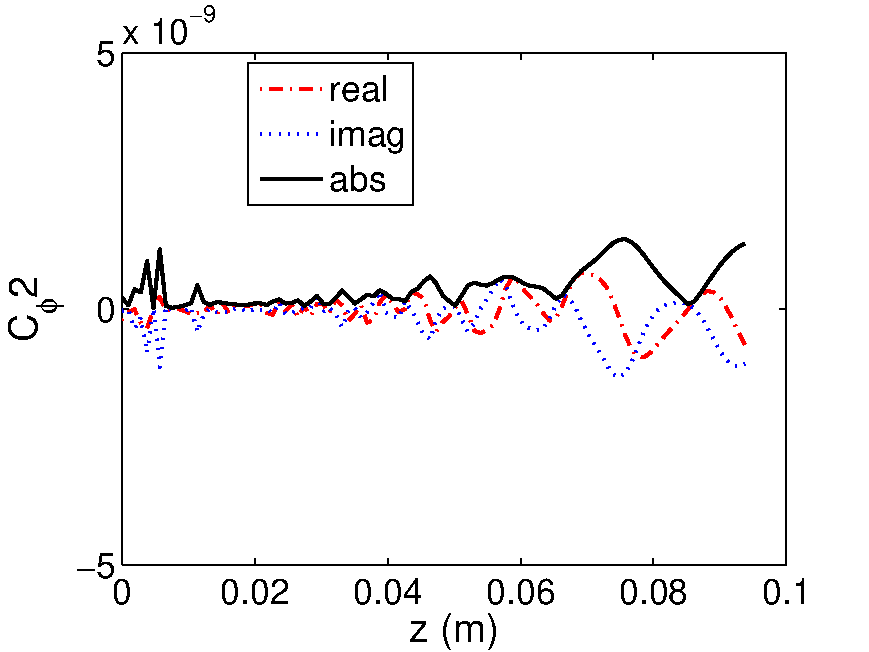
\includegraphics[scale=.44]{../media/Figs/Cphi2}}
\end{minipage}
\caption{$ \mathcal{C}^{(\omega,p=+,f=+)}(z) $. The values of these coefficients are in an arbitrary unit. }
\label{Cz}
\end{figure}




\begin{figure}[H] 
\centering
\subfloat[$ \mathcal{A}(z) $]{\label{Az}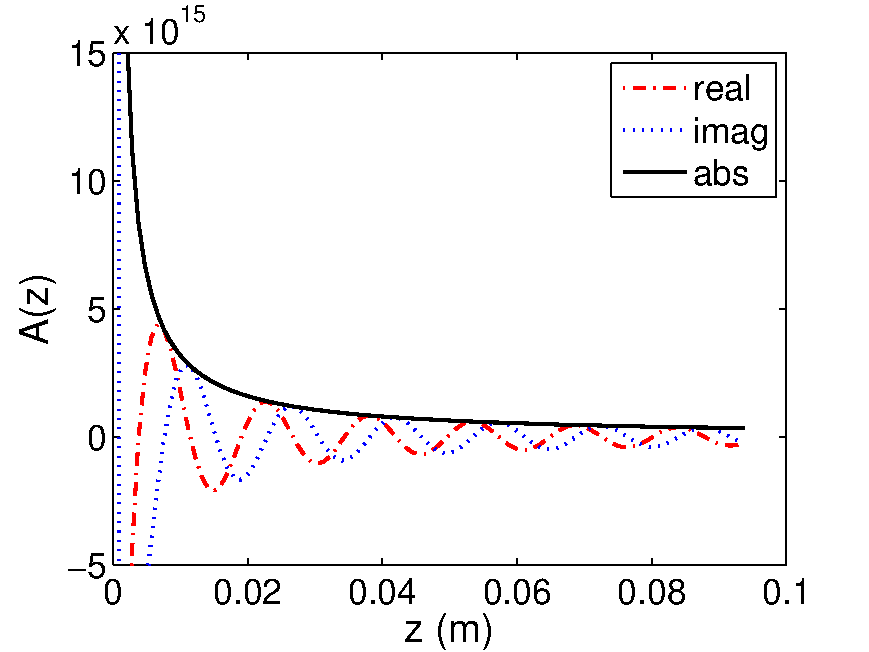
\includegraphics[scale=.5]{../media/Figs/Az}}
\par\medskip
\begin{minipage}{.5\linewidth}
\centering
\subfloat[$ \mathcal{C}_{r_\perp}(z) $]{\label{Crz}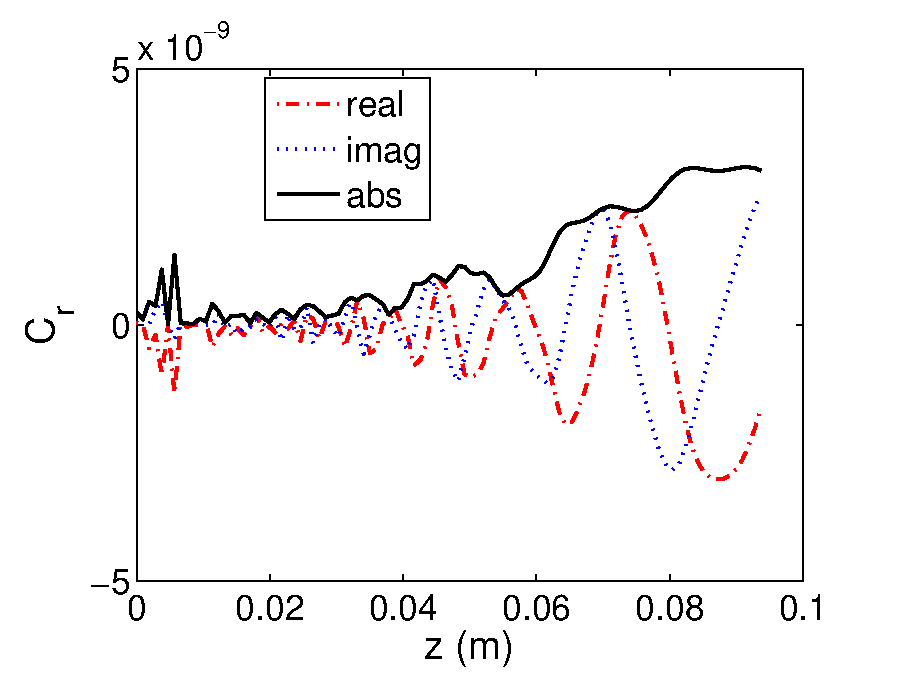
\includegraphics[scale=.44]{../media/Figs/Cr}}
\end{minipage}%
\begin{minipage}{.5\linewidth}
\centering
\subfloat[$ \mathcal{C}_\phi(z) $ ]{\label{Cphiz}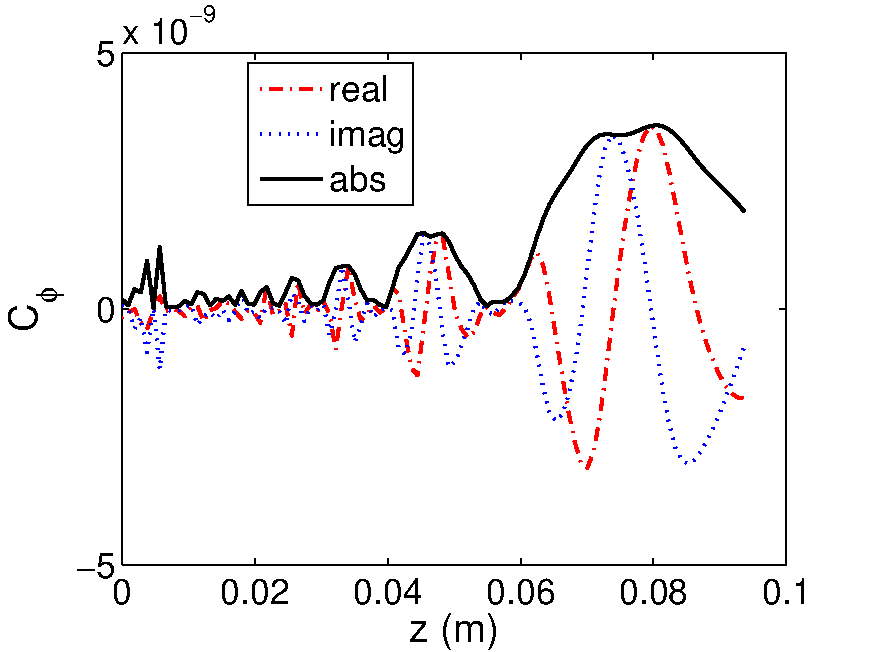
\includegraphics[scale=.44]{../media/Figs/Cphi}}
\end{minipage}
\par\medskip
\begin{minipage}{.5\linewidth}
\centering
\subfloat[$ \mathcal{S}_{r_\perp}(z) $ ]{\label{Srz}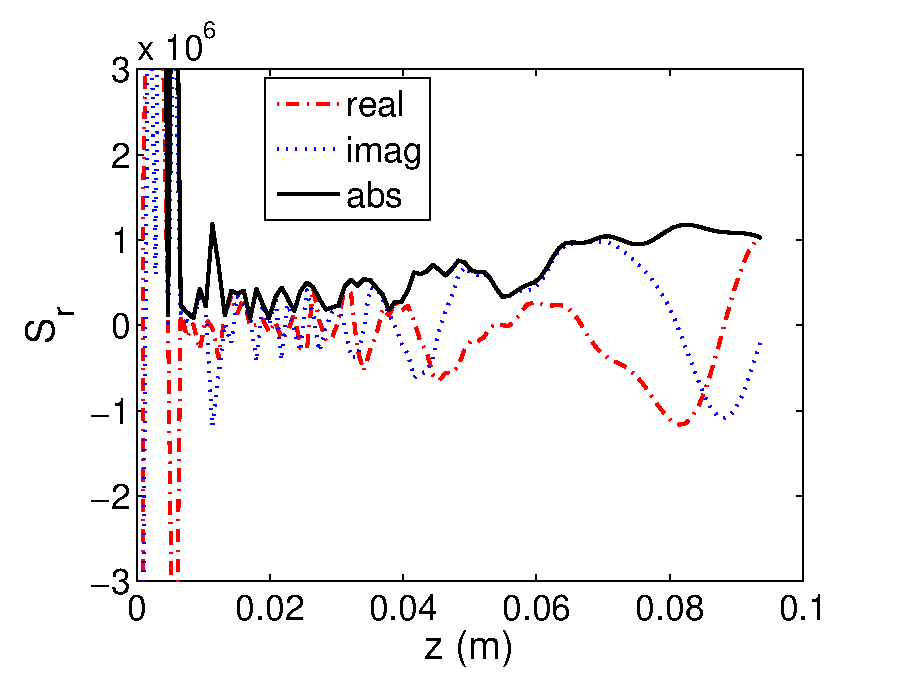
\includegraphics[scale=.44]{../media/Figs/Sr}}
\end{minipage}%
\begin{minipage}{.5\linewidth}
\centering
\subfloat[$ \mathcal{S}_\phi(z) $]{\label{Sphiz}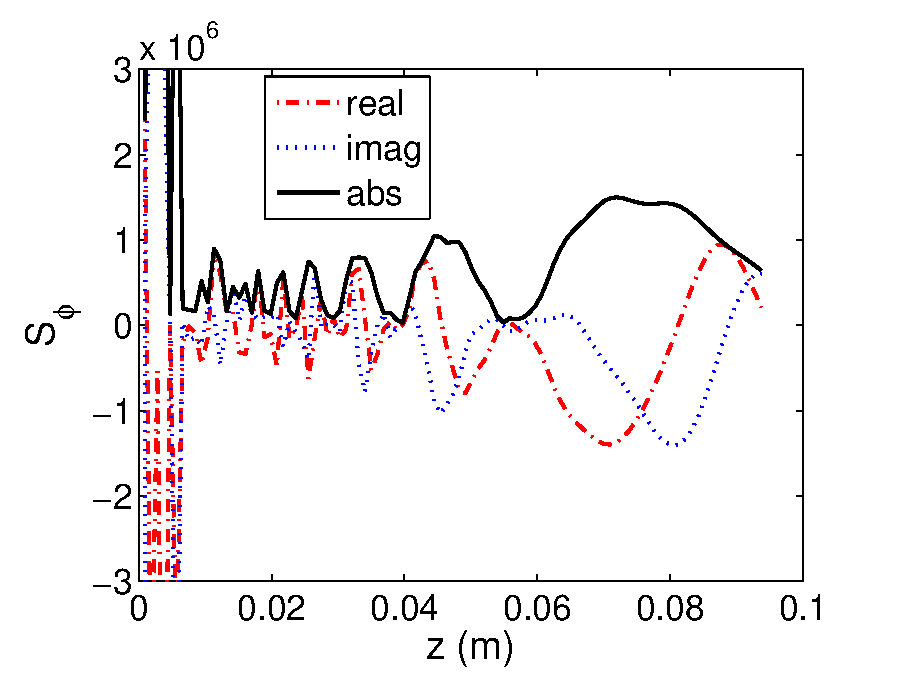
\includegraphics[scale=.44]{../media/Figs/Sphi}}
\end{minipage}
\caption{$ \mathcal{A}(z) $, $ \mathcal{C}^{(\omega,p=+,f=+)}(z) $ and $ \mathcal{S}^{(\omega,p=+,f=+)}(z) $. The values of these coefficients are in an arbitrary unit. There should be some fast chopping in $ \mathcal{A}(z) $ and $ \mathcal{S}^{(\mu)}(z) $. However, due to the cost of computing time, we did not give a fine enough calculation in our plots. See following plots for the calculation results with an improved resolution.  }
\label{ACSz}
\end{figure}


\scalefig{../media/Figs/InterferencePeriods}{0.6}{Wave path-difference of the interference between a monochromatic light emitted from a point atom located at $ \br'=(r'_\perp,\phi',z')=(2a,0,0) $ and a laser beam propagating along the $ z $-axis at the same wavelength $ \lambda_0=937.1 $ nm. The  horizontal axis of the plot is scaled in terms of the radium $ a $ of the nanofiber. The vertical axis is the wave path-difference measured along the laser's propagation direction of $ z $-axis, which is scaled by the wavelength $ \lambda=\lambda_0 $. As we can see, the interference period is uniform, and is on the order of $ 4.2a $.  This rough calculation implies that the chopping frequency in $ z $-direction should on the order of the wavelength, which should be reflected in Fig.~\ref{ACSz} and related plots. }


\newpage
Notice that, calculation resolution matters to the results. For comparison, we run the exact simulation as above but with a better $ z $-resolution.  The results are shown in Figs.~\ref{Cz_1} and~\ref{ACSz_1}. In $ z\in (0,1)\,\mathrm{mm} $ region, we calculate the coefficients in every $ 20 $ wavelengths; in $ z\in[2,100]\,\mathrm{mm} $ region, we calculate the coefficients in every $ \lesssim 1000 $ wavelengths. While in Figs.~\ref{Cz} and~\ref{ACSz} before, we calculate the coefficients evenly in every $ 1000 $ wavelengths. Also, when we calculated the integrals in the figures below, we used a $ 3 $ times better resolution in $ r_\perp\in(a,5a) $ region, which gives more detailed features of the $ \mathcal{C}^{(\mu)} (z)$ and $ \mathcal{S}^{(\mu)}(z) $ plots. With this improved resolution, it takes more than one hour to run the full calculation on a Thinkpad X200 laptop. 

\begin{figure}[H] 
\begin{minipage}{.5\linewidth}
\centering
\subfloat[$ \mathcal{C}_{r_\perp}(z) $ for $ r_\perp < a $]{\label{Cza_1}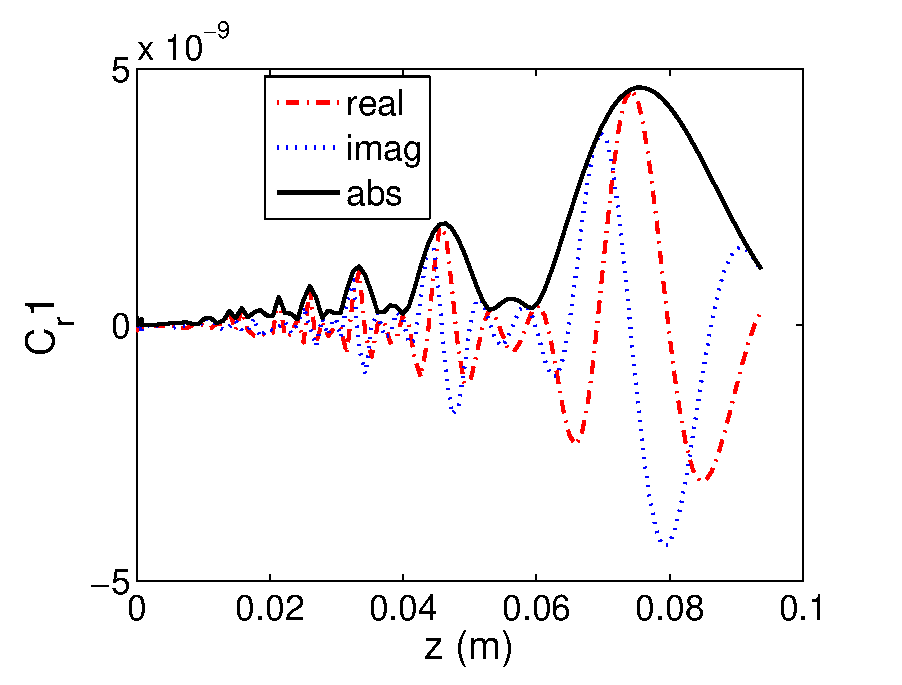
\includegraphics[scale=.44]{../media/Figs/Cr1_1}}
\end{minipage}%
\begin{minipage}{.5\linewidth}
\centering
\subfloat[$ \mathcal{C}_{r_\perp}(z) $ for $ r_\perp > a $]{\label{Czb_1}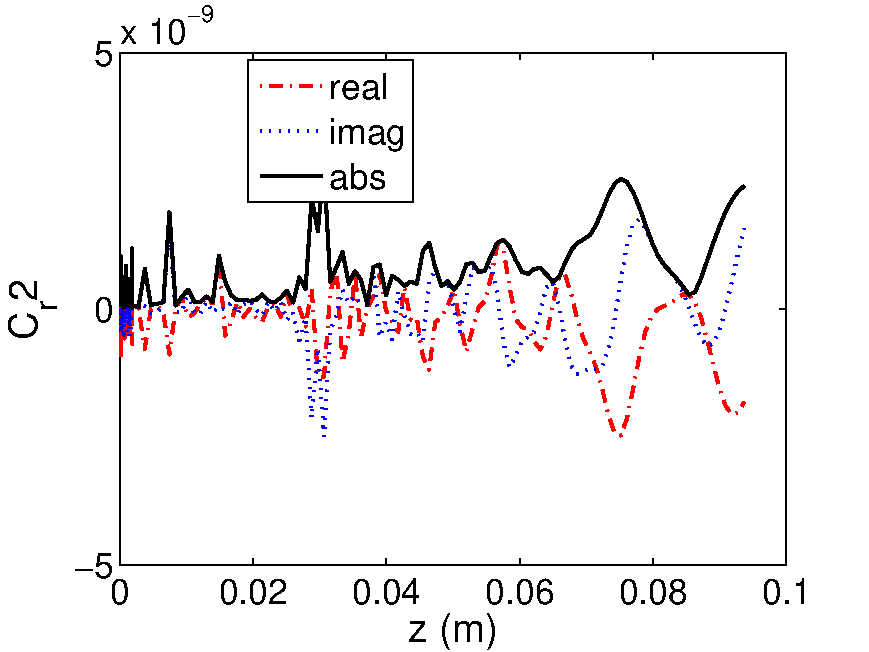
\includegraphics[scale=.44]{../media/Figs/Cr2_1}}
\end{minipage}
\par\medskip
\begin{minipage}{.5\linewidth}
\centering
\subfloat[$ \mathcal{C}_\phi(z) $ for $ r_\perp < a $]{\label{Czc_1}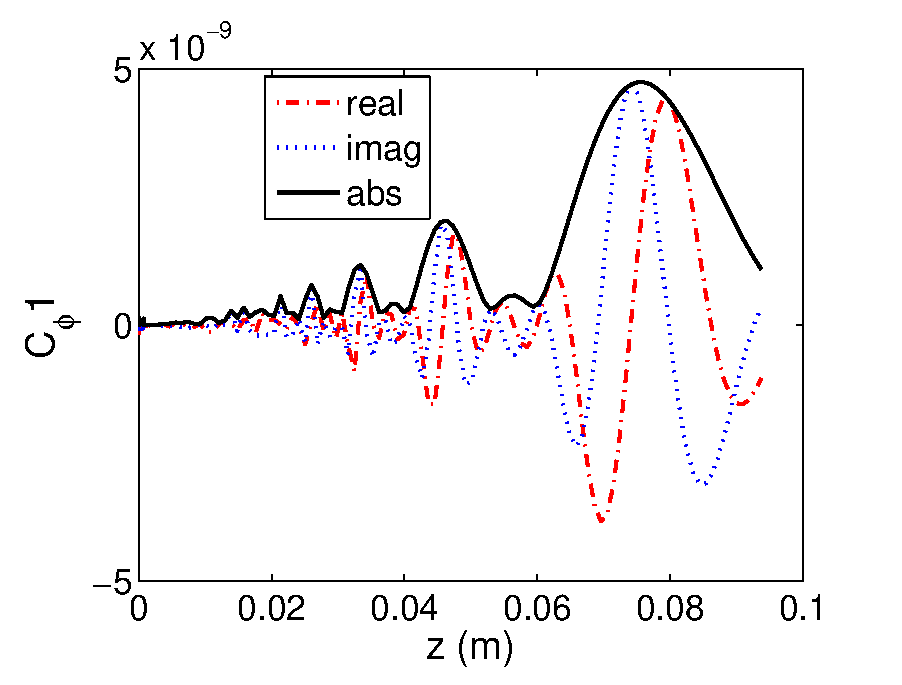
\includegraphics[scale=.44]{../media/Figs/Cphi1_1}}
\end{minipage}%
\begin{minipage}{.5\linewidth}
\centering
\subfloat[$ \mathcal{C}_\phi(z) $ for $ r_\perp > a $]{\label{Czd_1}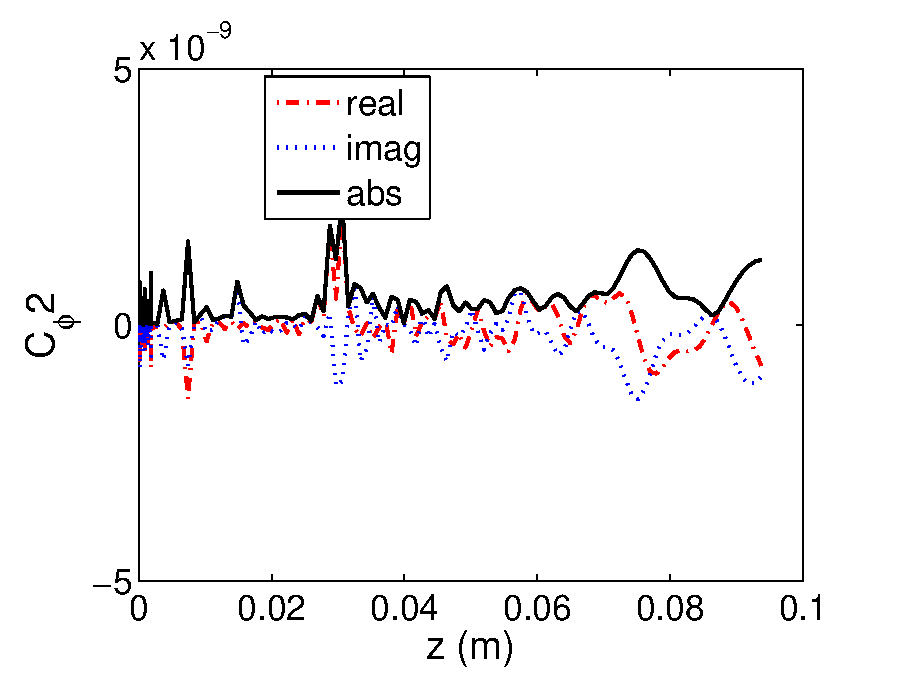
\includegraphics[scale=.44]{../media/Figs/Cphi2_1}}
\end{minipage}
\caption{$ \mathcal{C}^{(\omega,p=+,f=+)}(z) $. The values of these coefficients are in an arbitrary unit. Resolution is improved (see text).}
\label{Cz_1}
\end{figure}




\begin{figure}[H] 
\centering
\subfloat[$ \mathcal{A}(z) $]{\label{Az_1}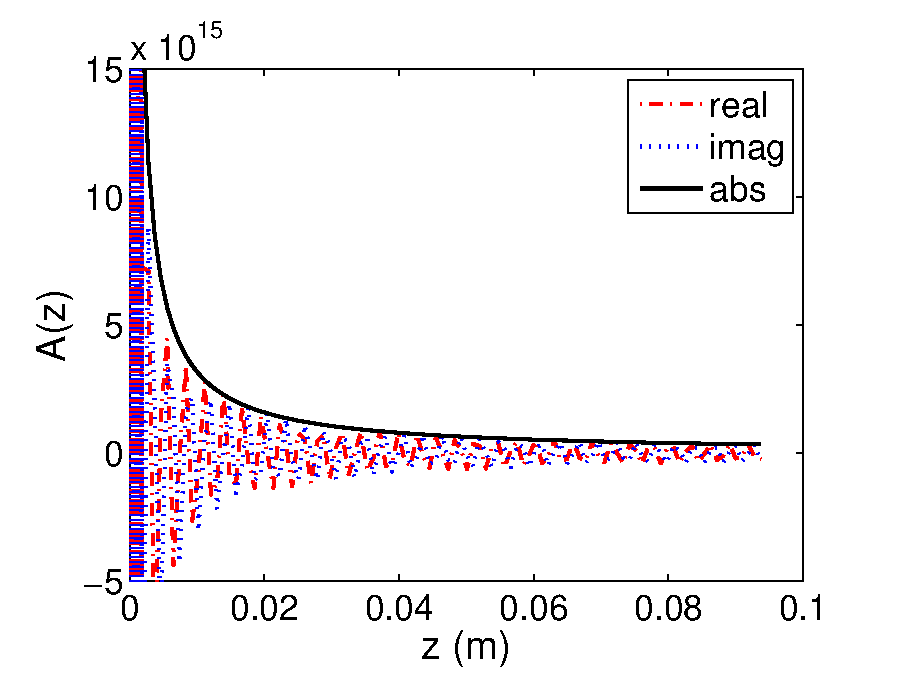
\includegraphics[scale=.5]{../media/Figs/Az_1}}
\par\medskip
\begin{minipage}{.48\linewidth}
\centering
\subfloat[$ \mathcal{C}_{r_\perp}(z) $]{\label{Crz_1}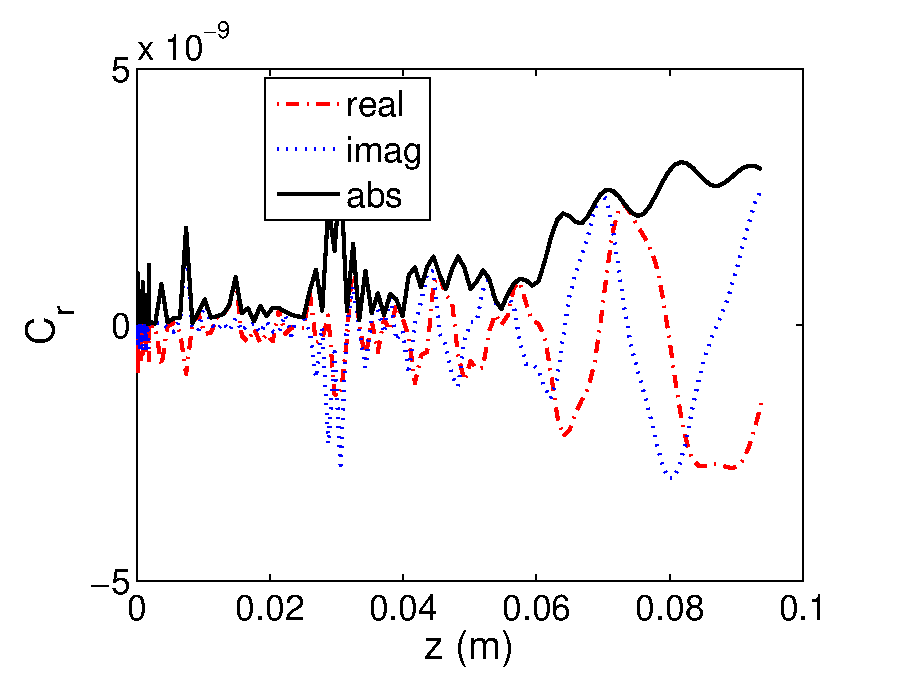
\includegraphics[scale=.42]{../media/Figs/Cr_1}}
\end{minipage}%
\begin{minipage}{.48\linewidth}
\centering
\subfloat[$ \mathcal{C}_\phi(z) $ ]{\label{Cphiz_1}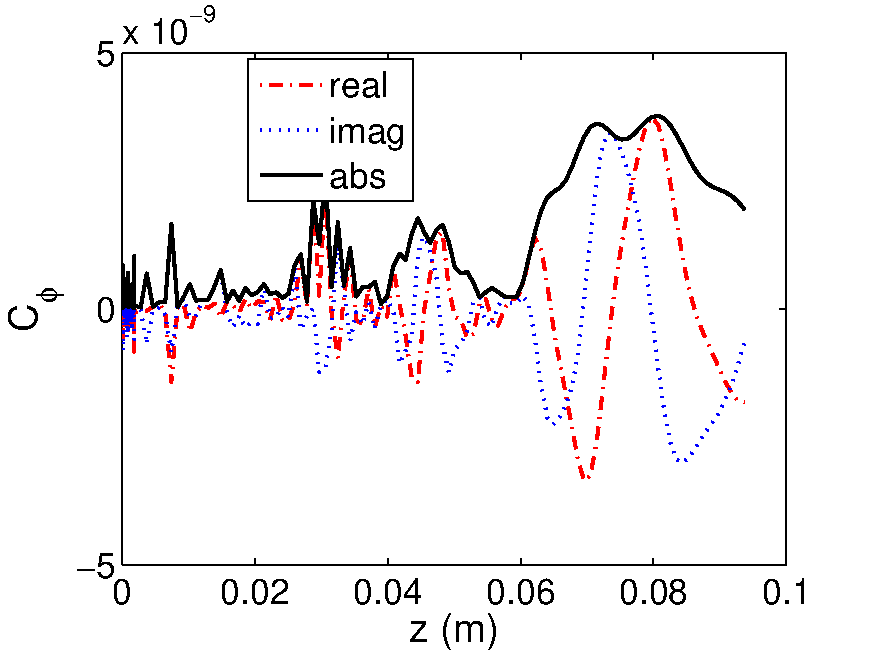
\includegraphics[scale=.42]{../media/Figs/Cphi_1}}
\end{minipage}
\par\medskip
\begin{minipage}{.48\linewidth}
\centering
\subfloat[$ \mathcal{S}_{r_\perp}(z) $ ]{\label{Srz_1}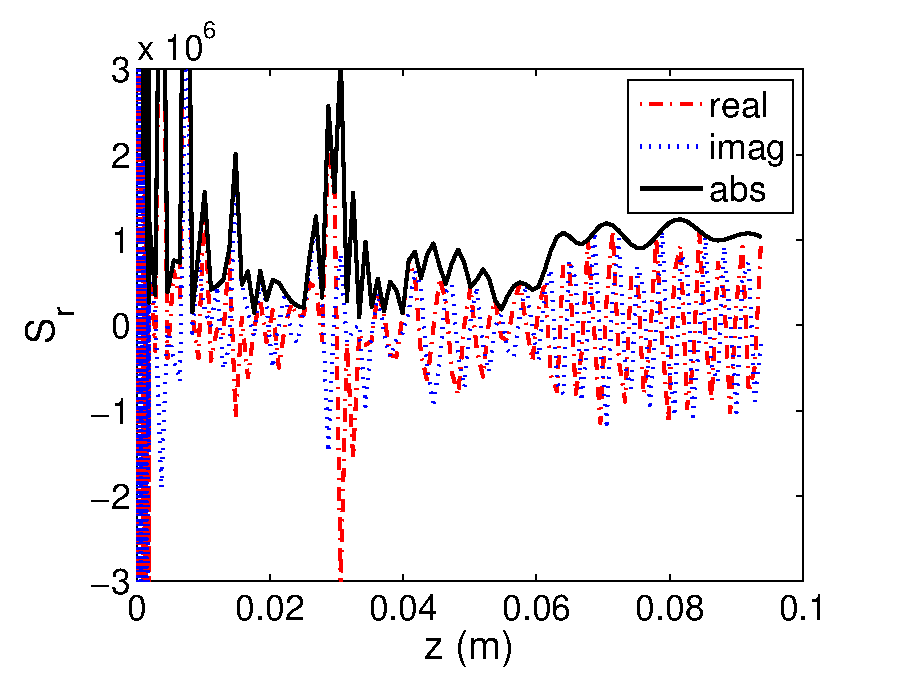
\includegraphics[scale=.42]{../media/Figs/Sr_1}}
\end{minipage}%
\begin{minipage}{.48\linewidth}
\centering
\subfloat[$ \mathcal{S}_\phi(z) $]{\label{Sphiz_1}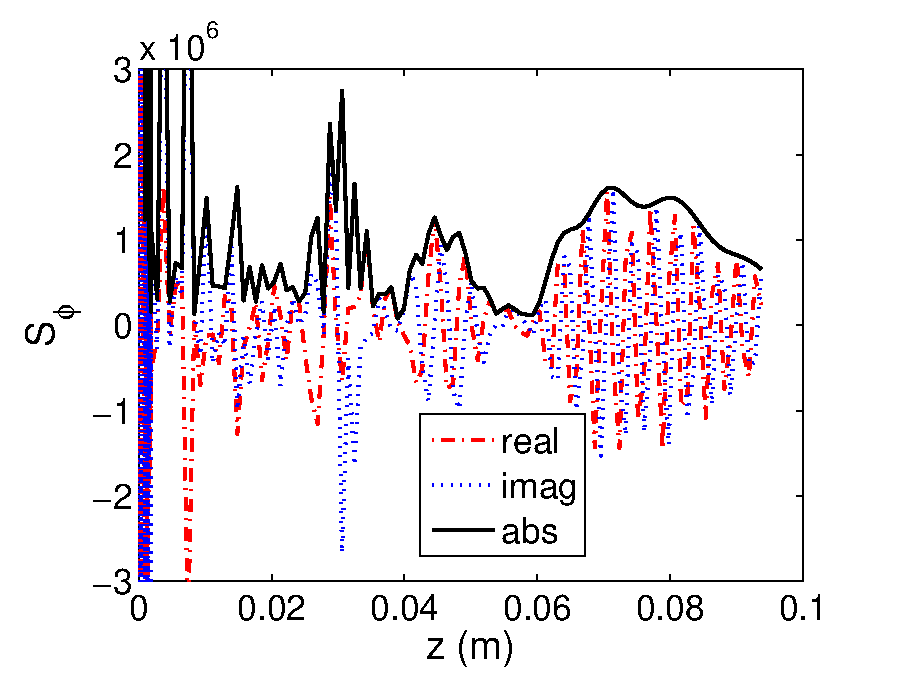
\includegraphics[scale=.42]{../media/Figs/Sphi_1}}
\end{minipage}
\caption{$ \mathcal{A}(z) $, $ \mathcal{C}^{(\omega,p=+,f=+)}(z) $ and $ \mathcal{S}^{(\omega,p=+,f=+)}(z) $. The values of these coefficients are in an arbitrary unit. Resolution is improved (see text).}
\label{ACSz_1}
\end{figure}



%\documentclass[fleqn, final]{../styles/unmphythesis}
\usepackage{../styles/qxd}
\renewcommand{\thechapter}{2}
%\newcommand{\thechapter}{1}

\makeindex
\begin{document}

%<*atomicphysicsformulas>

\chapter{Some useful formulas of atomic physics}\label{chap:summaryofatomicphysicsformulas}
We summarize some useful formulas for atoms presented in vacuum (including inside an optical cavity) in this appendix for us to generalize without proving some concepts for the nanophotonic waveguide case. We collect the formulas in various sources, which include but not limited to Refs.~\cite{Deutsch2010a,Kimble1998,Baragiola2014Open,Norris2014,Steck2007Quantum}.

\section{Spontaneous atomic decays}
Scalar polarizability of an atom:
\begin{align}
\alpha &=-\frac{|d_{eg}|^2}{\hbar (\Delta+i\Gamma/2)}, \,\, (\Delta=\omega-\omega_{eg}\equiv \omega-\omega_0),
\end{align}
where $ d_{eg} $ denotes the atomic momentum due to the dipole oscillations between $ \ket{g} $ and $ \ket{e} $ states, and $ \Gamma $ is the decay rate of the atom. In the dispersive interaction regime, one can usually ignore the imaginary part of the atomic polarizability as $ \Delta\gg \Gamma $~\cite{Deutsch2010a}, and hence
\begin{align}
\alpha \approx -\frac{|d_{eg}|^2}{\hbar\Delta}.
\end{align}

Decay rates (natural linewidth) of an atom in vacuum:
\begin{align}\label{eq:naturallinewidth}
\Gamma_{vac}=\Gamma_0 &= \frac{4}{3} \left( \frac{\omega_0}{c}\right)^3 \frac{|d_{eg}|^2}{\hbar}
\end{align}

When the atom is placed in a Gaussian laser field, the decay rate of the atom could be modified as
\begin{align}
\Gamma^{1D} &= \Gamma_g=2\pi \frac{|d_{eg}|^2}{\hbar A_{e\!f\!f}}\left(\frac{\omega_0}{c} \right),
\end{align}
where the scripts $ 1D $ and $ g $ indicate the effect is caused by the coupling to a quasi-1D propagating light field (guided), and $ A_{e\!f\!f} $ is the effective mode area of the beam. For commonly used atomic traps in free space, the TEM$_{00} $ mode is employed to probe atoms, which has an effective mode area given by
\begin{align}
A_{e\!f\!f} &= \frac{A}{|\mathbf{u}_{00}(\br')|^2}=\frac{A}{|\mathbf{u}_{00}(r'_\perp)|^2},
\end{align}
where $ \mathbf{u}_{00}(\br) $ is the TEM$_{00}$ mode of the Gaussian beam (see Appendix~\ref{chap:paraxialapproximation}), and $ A=\pi w_0^2/2 $ is the mode area at the $ z=0 $ plane with $ w_0 $ the waist radius of the mode. 

We define the resonant cross section of an atom to be
\begin{align}
\sigma_0 &= \frac{3\lambda^2}{2\pi}=\frac{6\pi}{k_0^2}=\frac{6\pi c^2}{\omega_0^2},
\end{align}
and then the decay rate due to the coupling to the laser beam can be rewritten as
\begin{align}\label{Gamma1DGammavac_appendix}
\Gamma^{1\!D} &= \frac{1}{4} \frac{\sigma_0}{A_{e\!f\!f}}\Gamma_0.
\end{align}
On the other hand, due to the dispersive interaction from the atom, the optical mode of the input TEM$_{00}$ Gaussian laser beam will also yield a phase shift, $ \delta \phi $, given by
\begin{align}
\delta\phi &=2\pi \frac{\omega_0}{c A_{e\!f\!f}} \re[\alpha] = 2\pi \frac{\omega_0}{cA} \re[\alpha] |\mathbf{u}_{00}(\br')|^2 =-\frac{1}{A} \sigma_0 |\mathbf{u}_{00} (r'_{\!\perp})|^2 \frac{\Gamma_{vac}}{4\Delta},
\end{align}
We can also write 
\begin{align}\label{phaseshiftGamma1D}
\delta\phi &= -2\pi \frac{|d_{eg}|^2}{\hbar \Delta} \frac{\omega_0}{cA_{e\!f\!f}}=-\frac{\Gamma^{1\!D}}{\Delta}.
\end{align}

In calculating the dipole moment of an atom, we use Eq.~\eqref{eq:opdmm'} based on the Wigner-Eckart theorem\index{Wigner-Echart theorem} to define the dipole moment amplitude of $ \hat{\mathbf{d}}_q $ by~\cite{Deutsch2010a}
\begin{align}
&\quad \bra{j'f'm'}\hat{\mathbf{d}}_q\ket{jfm} = o_{jf}^{j'f'}C_{f'm'}^{f,m;1,q} \bra{j'}\lvert d\rvert\ket{j}\\
&= (-1)^{f'+i+j'+1}\sqrt{(2j'+1)(2f+1)}\left\{ 
\begin{array}{ccc}
	f' & i & j' \\
	j & 1 & f
\end{array}\right\}C_{f'm'}^{f,m;1,q} \bra{j'}\lvert d\rvert\ket{j},
\end{align}
where we denote $ i $ as the nuclear spin number, $o_{jf}^{j'f'}$ as the relative oscillator strengths, $C_{f'm'}^{f,m;1,q}$ as the Clebsch-Gordan coefficients, and $\bra{j'}\lvert d\rvert\ket{j}$ as the reduced dipole matrix elements. 
Note that different research groups may define the transition amplitudes of the dipole operator in their own conventions, which leads to inconsistent definitions of the reduced matrix elements in literature.
In this dissertation, we can calculate the reduced matrix elements\index{reduced matrix element} using the experimentally measured partial lifetimes, $ \tau_{j'\!j} $, due to spontaneous emissions from $ j' $ to $ j $~\cite{Ding2012Corrections,McKeever2004,Arora2007Magic} by 
\begin{align}
|\bra{j'}\lvert d\rvert\ket{j}|^2 = \frac{3\pi \epsilon_0\hbar c^3}{\omega_{j'\!j}^3\tau_{j'\!j}},\label{eq:reducedmatrixelements}
\end{align}
where $ \epsilon_0 $ is the dielectric constant of vacuum, and $ \omega_{j'\!j} $ is the resonance frequency of the $ j'\rightarrow j $ transition.
Note, here we use the convention for the reduced dipole matrix element given by Wigner~\cite{Wigner1959Group} and Rose~\cite{Rose1957Elementary}.
Whilst, Refs.~\cite{Ding2012Corrections} and~\cite{LeKien2013} by Ding, Kimble, Le Kien, Rauschenbeutel, \textit{et al.}, for example, use the convention of Racah~\cite{Racah1942Theory,Fano1959Irreducible} and Edmonds~\cite{Edmonds1957Angular}.
Their definition of the reduced matrix elements' square is $ (2j'+1) $ times greater than ours. Ref.~\cite{Steck2007Quantum}, as another example, defines the square of the reduced dipole matrix elements as $(2j'+1)/(2j+1)$ folds of our definition, where $ j $ and $ j' $ are defined with respect to states of lower to higher energy, respectively, rather than with respect to initial to final states.


\section{Relationship between measurement strength and scattering rates}
To avoid using reduced dipole moment elements and other quantities in a wrong unit, we can normalize some quantities in terms of characteristic scattering rates and field intensities.
Here are some basic relationships.

Starting from the saturation parameter,
\begin{align}
S(\Delta ) &\equiv \frac{\Omega^2/2}{\Delta^2+\frac{\Gamma^2}{4}} = \frac{S(0)}{4\Omega^2/\Gamma^2+1} \approx \frac{\Omega^2}{2\Delta^2} \quad (\text{for $\Delta^2\gg \Gamma^2$})\\
S(0) &= \frac{I}{I_{\rm sat}}= \frac{2\Omega^2}{\Gamma^2}\\
I_{\rm sat} &= \frac{\hbar \omega}{\sigma_0} \frac{\Gamma}{2}.\label{eq:Isatsigma0}
\end{align}
Therefore, 
\begin{align}\label{eq:OmegaGamma}
\Omega^2 &= \frac{I}{I_{\rm sat}}\frac{\Gamma^2}{2}.
\end{align}


If we define a characteristic scattering rate as
\begin{align}
\gamma_s &\equiv \frac{\Gamma \Omega^2}{4\Delta_{\rm eff}^2},
\end{align}
then the relationships we have derived above (Eqs.~\ref{eq:OmegaGamma} and~\ref{eq:Isatsigma0}) will lead to
\begin{align}
\gamma_s &= \frac{\Gamma^3}{8\Delta_{\rm eff}^2} \frac{I}{I_{\rm sat}}\\
&= \sigma_0 \frac{\Gamma^2}{4\Delta_{\rm eff}^2}\frac{I}{\hbar \omega}.
\end{align}
This final step matches with the physical definition of $ \gamma_s $ that 
\begin{align}
\gamma_s &\equiv N_e \Gamma =\frac{S(\Delta_{\rm eff})}{2} \Gamma\\
&\equiv \sigma(\Delta_{\rm eff}) \frac{I}{\hbar \omega},
\end{align}
where $ \sigma(\Delta)=\frac{\sigma_0}{1+\frac{4\Delta^2}{\Gamma^2}}\approx \sigma_0 \frac{\Gamma^2}{4\Delta^2} $.

We define $ I=\frac{P}{A_{\rm in}}= \frac{\hbar \omega }{A_{\rm in}} \dot{N}_L $, and then
\begin{align}
\gamma_s &= \frac{\sigma_0 }{A_{\rm in}} \frac{\Gamma^2}{4\Delta_{\rm eff}^2}\dot{N}_L.
\end{align}

In a typical spin-squeezing case, the measurement strength may be given by
\begin{align}
\kappa &= \chi_{\rm eff}^2 \dot{N}_L,
\end{align} 
where $ \chi_{\rm eff}= \frac{\sigma_0}{A_{\rm eff}} \frac{\Gamma}{2\Delta_{\rm eff}} $.
Therefore,
\begin{align}
\kappa &= \frac{\sigma_0^2}{A_{\rm eff}^2} \frac{\Gamma^2}{4 \Delta_{\rm eff}^2} \dot{N}_L 
= \frac{A_{\rm in}\sigma_0}{ A_{\rm eff}^2}\gamma_s.
\end{align}


%As an example of spin-squeezing parameter calculation using the formulas above, we plot in Fig.~\ref{fig:QNDproperty_magic44} the optimal peak spin squeezing parameter (with various atom numbers) and OD-related parameters.
%
%\begin{figure}
%\begin{minipage}{.49\linewidth}
%\centering
%\subfloat[]{\label{fig:xi_optimal_NA1000to5000_omega44}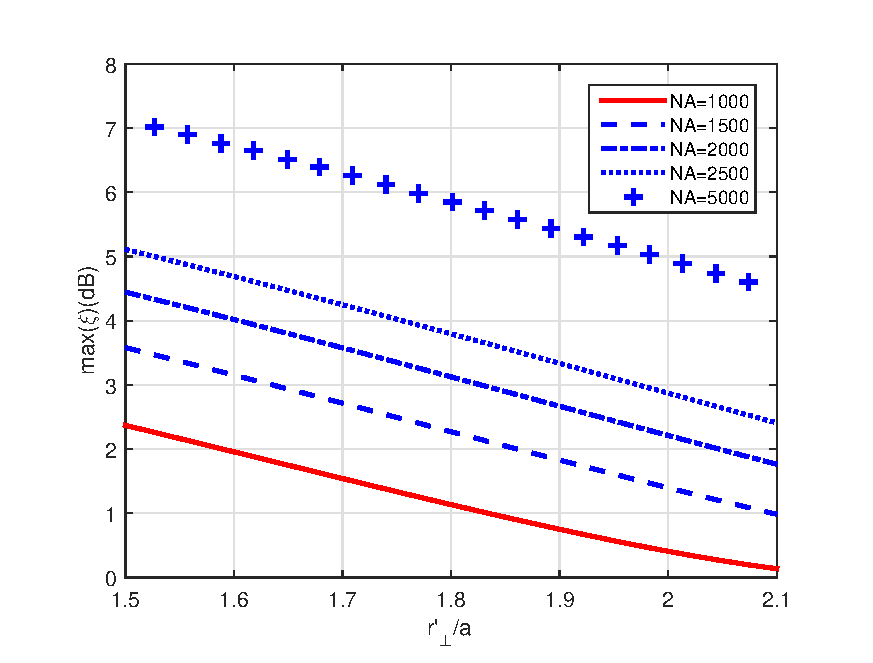
\includegraphics[scale=0.45]{./Figs/xi_optimal_NA1000to5000_omega44}}
%\end{minipage}
%\begin{minipage}{.49\linewidth}
%\centering
%\subfloat[]{\label{fig:OD_optimal_rp}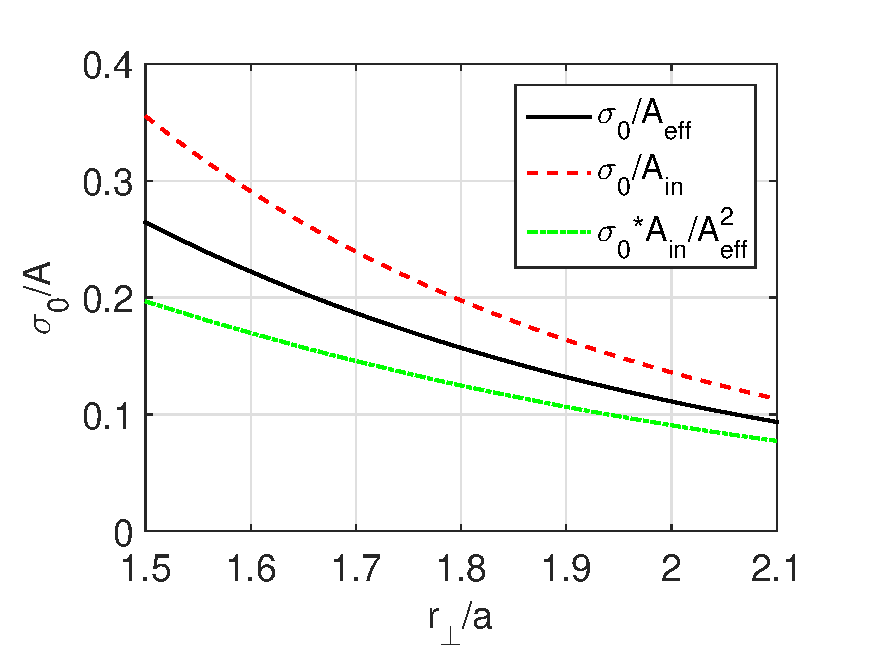
\includegraphics[scale=0.45]{./Figs/OD_optimal_rp}}
%\end{minipage}
%\caption{QND measurement properties using the magic frequency $ \omega_{44} $. Subfigure~\protect\subref{fig:xi_optimal_NA1000to5000_omega44} shows the optimal peak spin squeezing parameter as a function of the radial position of the atom. Different atom numbers have been indicated in different types of lines. Subfigure~\ref{fig:OD_optimal_rp} shows the OD per atom parameters and the ratio of $ \kappa/\gamma_s $ as a function of atoms' radial position when the optimal quantization axis is chosen to plot Subfig.~\protect\subref{fig:xi_optimal_NA1000to5000_omega44}.}\label{fig:QNDproperty_magic44}
%\end{figure}


\section{Relationship between OD/atom and cooperativity}
For atoms prepared in some state, the $\mathrm{OD}/\mathrm{atom}$ can be defined as
\begin{align}
\mathrm{OD}/\mathrm{atom} &= \frac{\sigma_0 }{A_{\rm eff} }, 
\end{align}
where the geometric property of the waveguide or optical medium and the inner structure property of the atoms have been absorbed into the effective mode area factor $ A_{\rm eff} $. 
While in cavity-QED, the concept of cooperativity is usually used to indicate the coupling strength between photons and atoms, and is equivalent to the cavity-to-free-space scattering ratio in the context of atomic cooling~\cite{Tanji-Suzukia2011,Vuletic2000,Kimble1998}. 
In this part, we want to show that the  $\mathrm{OD}/\mathrm{atom}$ in the context of traveling wave and atom interaction has an equivalent definition as the cooperativity in the context of optical cavity QED. 

Below, we consider a two-level atom interacting with an optical mode. 
From Eq.~\ref{Gamma1DGammavac_appendix} in the context of nanofiber geometry, we have
\begin{align}
\frac{\Gamma^{1\!D}}{\Gamma} &=   \frac{\sigma_0}{A_{\rm eff}}= \mathrm{OD}/\mathrm{atom}.
\end{align} 
The factor of $ \frac{1}{4} $ has been removed from Eq.~\ref{Gamma1DGammavac_appendix} when both propagating directions and polarizations of the modes are summed up in the equation above.

In the context of cavity-QED, the cooperativity per atom is defined as 
\begin{align}
C_1 &= \frac{2 g^2}{\kappa \Gamma},
\end{align}
where $ g=\frac{d\cdot E}{\hbar} $ is the coupling constant between the atom and the cavity mode with reduced dipole momentum $ \mathbf{d}=-e\bra{j}|\br|\ket{j'} $, and $ \kappa  $ and $ \Gamma $ are the decay rates of the cavity and atom respectively. 
One can use the relations that 
\begin{align}
E &= \sqrt{\frac{2\pi\hbar \omega}{V_{\rm eff}}}\\
V_{\rm eff} &= A_{\rm eff} L\\
\kappa &= \frac{c}{2L} \frac{1}{F}\\
\Gamma &= \frac{4}{3}\frac{\omega^3}{c^3} \frac{d^2}{\hbar}
\end{align}
where $ F $ is the cavity finesse.
The cooperativity can be then rewrite as
\begin{align}
C_1 &= \frac{4\pi d^2 \omega}{\hbar A_{\rm eff}L}\cdot  \frac{2L}{c}F \cdot \frac{3}{4} \frac{c^3}{\omega^3} \frac{\hbar}{d^2} = \frac{6\pi c^2}{\omega^2} \frac{1}{A_{\rm eff}} F\\
&= \frac{3\lambda^2}{2\pi} \frac{1}{A_{\rm eff}} F = \frac{\sigma_0}{A_{\rm eff}} F\\
&= \frac{\mathrm{OD}}{\mathrm{atom}} F.
\end{align}

For a Fabry–Pérot type cavity, the finesse is defined as the number of round trip a photon can make before leaking out, which only depends on the mirror reflectivity of the cavity. 
Alternatively, in terms of Q-factor, the finesse of a cavity can be written as $ F= Q\nu_F/\nu_0= Q \pi c/L\omega_0 $ with the Q-factor $ Q=\frac{\nu_0}{\delta\nu} $ and $ \nu_0 $ is the resonant frequency and $ \nu_F $ is the resonant frequency spacing~\cite{Saleh2007}. 
Giving a Gaussian mode with mode waist $ W_0 $, the cooperativity of an atom in the cavity becomes
\begin{align}
C_1 &= \frac{\sigma_0}{\pi W_0^2} F = \frac{\sigma_0}{A} F = \frac{\mathrm{OD}}{\mathrm{atom}} F.
\end{align}
This result agrees with literature~\cite{Hunger2010}. 

To increase the coupling strength between atoms and photons with a nanofiber, the atom number plays the role of cavity finesse in the context of optical cavity and relaxes the requirement of optical mode confinement in the dispersive regime. 

%</atomicphysicsformulas>

\bibliographystyle{../styles/abbrv-alpha-letters-links}
%\bibliographystyle{unsrt}
% \nocite{*}
\bibliography{../refs/Archive}

\printindex

\end{document}          
\ExecuteMetaData[../append/atomicformulas.tex]{atomicphysicsformulas}


\ExecuteMetaData[../chap3/QuantumDynamics.tex]{basistransfHS}


\ExecuteMetaData[../chap4/Birefringence.tex]{atomnumberdetection}

\chapter[Finding the magic wavelength for the birefringence protocol]{Finding the magic wavelength for the birefringence QND measurement and spin squeezing protocol for clock-state atoms trapped around a nanofiber}\label{chap:magicwavelength}
In this appendix, we provide some details on finding the magic frequency so that the photon fluctuation noise can be canceled while a QND-measurement-useful Hamiltonian can be retained. We first prove that in the case of one-frequency probe, the scalar polarizability of atoms doesn't allow a magic wavelength for our purpose; then we show that if the scalar polarizability has to be used (for example, to avoid photon scatterings among atoms), a two-color scheme may be feasible; finally, we provide some details on calculating the magic wavelength with one-color probe considering the tensor polarizability effect. We will only take the example of nanofiber, but the theory can be generalized to other nanophotonic waveguides.

Based on Chapter~\ref{chap:birefringence}, in the case that a nanofiber dispersively coupled to an atomic ensemble, the Hamiltonian per time $ \tau $ measurement can be given as below using the Stokes operators, $\hat{S}_q $, and collective spin operators, $ \hat{J}_q $, with $ q=0,1,2,3 $:
\begin{align}
H_{\rm eff} 
=\frac{\hbar}{\tau} \Big\{ & \left[ \big( \chi_{H,\uparrow} + \chi_{H,\downarrow}\big) + \big(\chi_{V,\uparrow} + \chi_{V,\downarrow}\big) \right] \hat{J}_0 \hat{S}_0 \nonumber \\
+ & \left[ \big( \chi_{H, \uparrow} + \chi_{H,\downarrow}\big) - \big( \chi_{V,\uparrow} + \chi_{V,\downarrow} \big)\right]  \hat{J}_0 \hat{S}_1 \nonumber \\
+ & \left[ \big( \chi_{H,\uparrow} - \chi_{H,\downarrow}\big) + \big(\chi_{V,\uparrow} - \chi_{V,\downarrow} \big) \right] \hat{J}_3 \hat{S}_0 \nonumber \\
+ & \left[ \big( \chi_{H,\uparrow} - \chi_{H,\downarrow}\big) - \big(\chi_{V,\uparrow} - \chi_{V,\downarrow} \big) \right]  \hat{J}_3 \hat{S}_1\Big\}.\label{eq:JScoupling}
\end{align}
If we want to estimate the state of the collective 
spins, we need to estimate the number of atoms sitting in the $ \ket{\uparrow} $ and $ \ket{\downarrow} 
$ states employing a dispersive QND measurement technique which has been well developed for the 
free-space atomic ensembles. For our system, the forth term of the Hamiltonian in 
Equ.~\eqref{eq:JScoupling} empowers us the possibility of measuring the atomic states without 
destroying them with an $ \hat{S}_3=\frac{1}{2i}(\hat{a}_H^\dagger\hat{a}_V - 
\hat{a}_V^\dagger\hat{a}_H) $ homodyne measurement. Yet, the third term of the Hamiltonian becomes 
a source of noise term that brings in photon number fluctuation noise into the measurement result. We want to find a magic wavelength of the probe light which allows us to totally remove the third term. For simplicity, we call the third line of the Hamiltonian as $ \hat{H}^3_{\rm eff} $ and its coefficient before the $ \hat{J}_3\hat{S}_0 $ or the corresponding coupling strength as $ \chi_3 $; similarly, we label with the number $ 4 $ for the fourth term of the Hamiltonian and its strength of coupling. We also denote the coupling strength in the fourth term of the Hamiltonian as $ \chi_{\rm eff} $ for the purpose of designing the measurement protocol.


\section{Magic wavelength does not exist with merely scalar polarizability using a simple strategy}
First, we look at the case that the atomic polarizability tensor is reduced to a scalar, which maintain the polarization state of the light in the process of interaction. There are many ways to physically realize such an effect for atoms. 
Here, we assume the detuning of the optical field is much larger than the natural linewidth of the 
coupled atoms so that we can ignore the tensor contribution of the atomic polarizability. We have also 
restricted the atomic ground state within the $ 6S_{1/2} $ $ F=3 $ ($ \ket{\downarrow} $) and $ F=4 $ ($ 
\ket{\uparrow} $) clock state space\index{state!clock state} which rules out the vector contribution of 
the atomic polarizability. Therefore, the atomic polarizability only has a scalar polarizability effect for this problem. 

From the definition of the coupling strength of various $ \chi $'s (Equs.~\eqref{chiHUp} through~\eqref{eq:AeffV}), one can show that, for $ D_1 $ line, 
\begin{align}
\chi_H \equiv \chi_{H,\uparrow} - \chi_{H,\downarrow} &= \frac{1}{3}\sum_{f'} \left(\frac{\sigma_0}{A_{\rm eff}^H} \right) \left(\frac{\Gamma}{4\Delta_{4f'}} - \frac{\Gamma}{4\Delta_{3f'}} \right) \nonumber\\
&= \frac{\Gamma_H}{3} \left(\frac{1}{\Delta_{43}}+\frac{1}{\Delta_{44}} - \frac{1}{\Delta_{33}}-\frac{1}{\Delta_{34}} \right) = \frac{\Gamma_H}{3}\Delta_-,\label{eq:chiH}\\
\chi_V \equiv \chi_{V,\uparrow} - \chi_{V,\downarrow} &= \frac{1}{3}\sum_{f'} \left(\frac{\sigma_0}{A_{\rm eff}^V} \right) \left(\frac{\Gamma}{4\Delta_{4f'}} - \frac{\Gamma}{4\Delta_{3f'}} \right) \nonumber\\
&= \frac{\Gamma_V}{3} \left(\frac{1}{\Delta_{43}}+\frac{1}{\Delta_{44}} - \frac{1}{\Delta_{33}}-\frac{1}{\Delta_{34}} \right)=\frac{\Gamma_V}{3}\Delta_-,\label{eq:chiV}
\end{align}
where $ \Delta_{ff'} $ is the detuning relative to the $ f\leftrightarrow f' $ transition gap, and $ \Delta_- = \left(\frac{1}{\Delta_{43}}+\frac{1}{\Delta_{44}} - \frac{1}{\Delta_{33}}-\frac{1}{\Delta_{34}} \right) $ is a common factor existing in both $ \chi_H $ and $ \chi_V $ quantities. $ \Gamma_H $ ($ \Gamma_V $) is the decay rate coupled to the forward propagating $ H $ ($ V $) mode of the nanofiber. 

To find the \emph{magic wavelength}\index{magic wavelength}, we need to make the coupling strength factor of the third term of the Hamiltonian in Equ.~\eqref{eq:JScoupling} equal to zero. That is to say,
\begin{align}
\chi_H+\chi_V=\frac{1}{3}\left(\Gamma_H + \Gamma_V \right)\Delta_- = 0.
\end{align}
We can see that $ \frac{1}{3}\left(\Gamma_H + \Gamma_V \right) $ is always positive and does not 
depending on wavelength. Therefore, we have to let $ \Delta_-=0 $ to find the "\textit{magic 
wavelength}"\index{magic wavelength}. From the definition of $ \chi_H $ and $ \chi_V $ 
(Equs.~\eqref{eq:chiH} and~\eqref{eq:chiV}) and the Hamiltonian (Equ.~\eqref{eq:JScoupling}), we can 
find that $ \chi_H=\chi_V=0 $ and the forth term of the Hamiltonian, which is what we want to keep, also 
becomes zero. Hence, via identifying a magic wavelength and to remove the photon flux noise in the 
measurement is invalid for our initial design. Maybe we can say, the \emph{magic wavelength}\index{magic wavelength} does not 
exist for one-color probe configuration and by only considering scalar polarizability effects. 

This analytical conclusion has been numerically verified. 

\section{Calculating coupling strengths with a scalar polarizability}
Now, let us suppose we target to generating a spin squeezed state (SSS) based on the forth term of the Hamiltonian through an $ \hat{S}_3 $ homodyne QND measurement. The effective Hamiltonian becomes
\begin{align}
	H_{\rm eff} = \frac{\hbar}{\tau} \chi_{\rm eff} \hat{J}_3 \hat{S}_1
\end{align}
where $\chi_{\rm eff} = \chi_{H} - \chi_{V}=\frac{\Gamma_H-\Gamma_V}{3}\Delta_-$. As has been proved, the squeezing parameter $ \xi =\frac{\chi_{\rm eff}^2 }{4}N_LN_A $. Therefore, to calculate the squeezing parameter, we need to calculate the decay rates coupled into the $ H $ and $ V $ modes. 

Since we can treat the atomic polarizability as a scalar for our dispersive case, we have 
\begin{align}
\Gamma_H &= 2\pi \sum_g \frac{|\mathbf{u}_H(\br')\cdot \mathbf{d}_{eg}|^2}{\hbar}\left(\frac{\omega_0}{v_g} \right) \\
&\propto \sum_g \tr \left\{(\mathbf{d}_{eg}^*\mathbf{d}_{eg})\cdot \mathrm{Im} [\GFT_H^*(\br',\br')] \right\}  = \sum_f \tr \left[ \alpha_f \eye\cdot \mathrm{Im} [\mathbf{G}_H^*(\br',\br')]  \right],
\end{align}
where the atomic polarizability for the ground state $ f $ is defined as $ \alpha_f=\alpha_0(\Delta_{ff'})C_{j'f}^{(0)} $ is a scalar constant for the clock state. Using the emission surface technique introduced in Sec.~\ref{sec:geometryofemission}, the equivalent dipole momentum is pointed along $ [1,1,1]/\sqrt{3} $ direction on the principle emission coordinate system induced by the fiber $ H $-mode field. Since the $ H $ mode only has $ r\!_\perp $ and $ z $ components for an atom on the $ H $ axis, the field only couples to the corresponding $ \mathbf{e}_x $ and $ \mathbf{e}_z $ two dipole orientations with a normalization factor $ 1/3 $ for the $ D_1 $ line transitions. Similar conclusion applies to the $ \Gamma_V $ calculation yet with a $ y $ coupling. One can also consider this problem in the perspective of quantum jumps. Since all quantum transitions ($ \pi$ and $\sigma_\pm $) have the same possibility ($C_{j'ff'}^{(0)}=C_{j'f}^{(0)}=1/3 $), the decay rate is only determined by the non-zero field components with corresponding quantum transition probability. The final result does not depend on how we define the quantization axis while the details of calculation might be. 



With the knowledge of the equivalent dipole orientations, we can easily calculate the corresponding decay rates goes into the forwarding $ H $ and $ V $ modes respectively using the dipole approximation of the atom. Plots below (Figs.~\ref{fig:HVdecayrates} and~\ref{fig:squeezingparaTerms}) illustrate the decay rates and the normalized squeezing parameter $ \xi/N_LN_A $ as functions of frequency and atom positions relative to the fiber axis. $ N_L $ is the photon number counted through the photon detector during time $ \tau $ of measurement. Note that we have assumed that the decay rate is a constant within the small detuning around the D1 line transition frequency, which should be valid. Also, in Fig.~\ref{fig:squeezingparaTerms}, we made up a toy model that we assume both the third and fourth lines of the Hamiltonian alone can generate some spin squeezing with respect to $ \hat{J}_3 $ by some "technical" measurement strategies in time $ \tau $. We plot out the squeezing parameters associated with those two Hamiltonian terms in (a) and (b) of Fig.~\ref{fig:squeezingparaTerms}. If both (a) and (b) have similar values at the same frequency and atom position points, it means the coupling effect to both Hamiltonians overlap and the useful spin squeezing with the realistic Hamiltonian (in presence of both Hamiltonian terms) will be weak. If there are mismatches on the data points, in contrast, it means one can design some protocol to obtain a strong spin squeezing effect. Based on the plots, one can hardly design a good spin squeezing protocol based on the properties of the Hamiltonian. 

\begin{figure}[!tbp]
\begin{minipage}{.91\linewidth}
\centering
{\includegraphics[scale=0.75]{../media/Figs/HVdecayrates}}
\end{minipage}
\caption[Decay rates coupled to the $ H $ and $ V $ nanofiber modes with a scalar polarizability of atoms.]{Decay rates coupled to the $ H $ and $ V $ nanofiber modes. For the guided mode contributions, only the forward propagating mode contributions are plotted out. The total decay rates for the two mode contributions have both backward and forward propagating components counted.}\label{fig:HVdecayrates}
\end{figure}

\begin{figure}[!tbp]
\begin{minipage}{.91\linewidth}
\centering
\subfloat[]{\label{squeezingparaTerm3}\includegraphics[scale=0.55]{../media/Figs/squeezingparaTerm3}}
\end{minipage}
\par\medskip
\begin{minipage}{.91\linewidth}
\centering
\subfloat[]{\label{squeezingparaTerm4}\includegraphics[scale=0.55]{../media/Figs/squeezingparaTerm4}}
\end{minipage}
\caption[Squeezing parameters as a function of frequency and the atoms' radial position using a scalar polarizability in a toy model.]{Squeezing parameters associated with the third (a) and forth (b) terms of the Hamiltonian as a function of frequency and the atoms' radial position (see text). The colormap shows the value of $ -10\log_{10}(\xi/N_LN_A) $, where $ \xi $ is the squeezing parameter and $ N_L $ is the photon number counted at the photon detector in time period $ \tau $. The calculation assumes the signal is solely generated by $ \hat{H}^3_{\rm eff} $ and $ \hat{H}^4_{\rm eff} $, respectively, which is just a toy model. We use this simulation to show the possibility of designing a good spin squeezing protocol by finding a proper frequency and some atom positions. }
\label{fig:squeezingparaTerms}
\end{figure}

\begin{figure}
\begin{minipage}{.91\linewidth}
\centering
{\includegraphics[scale=0.75]{../media/Figs/chi34}}
\end{minipage}
\caption[Coupling strengths as a function of detuning.]{The coupling strengths for the third ($ \chi_3 $) and forth ($ \chi_4 $) terms of the Hamiltonian expressed in Eq.~\eqref{eq:JScoupling} for the D1 line transitions associated with the clock states.} \label{fig:chi34}
\end{figure}

As shown in Fig.~\ref{fig:chi34} regarding the coupling strengths of the third and forth terms of the one-color probe Hamiltonian, the two peaks on the negative frequency side and those on the positive frequency side correspond to the approximate frequencies one can use to detect the $ \ket{\uparrow} $ and $ \ket{\downarrow} $ atom numbers. The two Hamiltonian terms seem very close to each other due to the small $ \Gamma_V $. How much the photon fluctuation affects the final result is unclear, but the noise is on the same order as the signal (projection noise).



\section{Estimate psuedo-spin state and atom number in a high resolution}
Now we come to the question "is there any way to remove the photon fluctuation from the homodyne measurement?" One way that might work is to use two-color light signals to commit the measurement. The basic idea follows. 

If we use two-color probes for each measurement configuration, it might be possible to find non-trivial magic wavelengths to cancel the third term of the Hamiltonian. The key is that, for two distinguishable colors, the decay rates coupled to the corresponding guided modes are distinguishable as well, which may result in magic wavelengths that does not totally remove the coupling strengths at the same time. For instance, if we choose the two probes around D1 and D2 transition frequencies at $ \omega_1 $ and $ \omega_2 $, the two sets of $ \Gamma_{H/V}(\omega_1) $ and $ \Gamma_{H/V}(\omega_2) $ will be different. Quantitatively, the third term of the effective Hamiltonian can now be given by
\begin{align}
\!\!\!\!\!\!\!\!\!\!\hat{H}_{\rm eff}^3(\omega_1,\omega_2) &= \frac{\hbar}{\tau} \left[\chi_H(\omega_1)+\chi_H(\omega_2) + \chi_V(\omega_1)+\chi_V(\omega_2) \right] \hat{J}_3\hat{S}_0\\
&= \frac{\hbar}{3\tau} \left[  \left( \Gamma_H(\omega_1)\!+\!\Gamma_V(\omega_1) \right)\Delta_-^1(\omega_1) \!+\! 2\left( \Gamma_H(\omega_2)\!+\!\Gamma_V(\omega_2) \right)\Delta_-^2(\omega_2) \right] ,
\end{align}
where $ \Delta_-^{1/2} $ are the detuning terms due to the two colors of the probes. Similarly, the forth term of the Hamiltonian can now be given by
\begin{align}
\!\!\!\!\!\!\!\!\!\!\hat{H}_{\rm eff}^4(\omega_1,\omega_2) &= \frac{\hbar}{\tau} \left[\chi_H(\omega_1)+\chi_H(\omega_2) - \chi_V(\omega_1)-\chi_V(\omega_2) \right] \hat{J}_3\hat{S}_0\\
&= \frac{\hbar}{3\tau} \left[  \left( \Gamma_H(\omega_1)\!-\!\Gamma_V(\omega_1) \right)\Delta_-^1(\omega_1) \!+\! 2\left( \Gamma_H(\omega_2)\!-\!\Gamma_V(\omega_2) \right)\Delta_-^2(\omega_2) \right] .
\end{align}
Now that, the magic wavelengths canceling the third term of the Hamiltonian may not result in a zero coupling strength for the forth term of the Hamiltonian due to the inseparability of decay rates and detuning factors. A two-color scheme has been tested in experiments by the QUANTOP group in Denmark for QND measurement~\cite{Beguin2014}, but it's more about using the differential phase shifts between the two probes to magnify the signal-to-noise ratio than using an precise magic wavelength to cancel the noise sources. 


\section{Magic wavelength exists by including tensor polarizability effect}
Finally, if we include the tensor polarizability effect into the Hamiltonian, and use the $ x $-axis as the 
quantization axis, the Hamiltonian can still be given in the form of Eq.~\ref{eq:JScoupling} yet with a 
tensor-response definition of the coupling strengths:
\begin{align}
\chi_{H,\uparrow/\downarrow} & \equiv \chi_{H,f} =- \frac{2\pi \omega_0}{v_g} \bra{f,0} 
	\mathbf{u}^*_H(r^\prime\!_\perp, \phi') \cdot \tensor{\alpha} \cdot 
	\mathbf{u}_{H}(r^\prime\!_\perp, 
	\phi') \ket{f,0} \\
	& =- \frac{2\pi \omega_0}{v_g} \sum_{f'} \sum_q \alpha_0\left( f,f'  \right) |\mathbf{e}_q \cdot 
	\mathbf{u}_H^*(r^\prime\!_\perp,\phi')|^2 |o^{j'f'}_{jf} |^2 
	|C^{f 0;1q}_{f' q}|^2\\
	& \approx  \frac{1}{2} \left( \sigma_0 n_g  \right) \sum_{f'} \sum_q\left( 
		\frac{\Gamma}{2 
		\left(\Delta_{f,f'}+i\Gamma/2\right) }  \right)\nonumber\\
		&\quad\quad\quad\quad\quad\quad\quad\quad\quad \times |\mathbf{e}_q \cdot 
		\mathbf{u}_H^*(r^\prime\!_\perp,\phi')|^2 |o^{j'f'}_{jf} |^2 
		|C^{f 0;1q}_{f' q}|^2,\\
\chi_{V,\uparrow/\downarrow} & \equiv \chi_{V,f} =- \frac{2\pi \omega_0}{v_g} \bra{f,0} 
	\mathbf{u}^*_V(r^\prime\!_\perp, \phi') \cdot \tensor{\alpha} \cdot 
	\mathbf{u}_{V}(r^\prime\!_\perp, 
	\phi') \ket{f,0} \\
	& =- \frac{2\pi \omega_0}{v_g} \sum_{f'} \sum_q \alpha_0\left( f,f'  \right) |\mathbf{e}_q \cdot 
	\mathbf{u}_V^*(r^\prime\!_\perp,\phi')|^2 |o^{j'f'}_{jf} |^2 
	|C^{f 0;1q}_{f' q}|^2\\
	& \approx  \frac{1}{2} \left( \sigma_0 n_g  \right) \sum_{f'} \sum_q\left( 
		\frac{\Gamma}{2 
		\left(\Delta_{f,f'}+i\Gamma/2\right) }  \right)\nonumber\\
		&\quad\quad\quad\quad\quad\quad\quad\quad\quad \times |\mathbf{e}_q \cdot 
		\mathbf{u}_V^*(r^\prime\!_\perp,\phi')|^2 |o^{j'f'}_{jf} |^2 
		|C^{f 0;1q}_{f' q}|^2,
\end{align}
where we have approximated $ \lambda_{j'}\approx \lambda = \frac{2\pi c}{\omega_0} $.  

The magic wavelengths/frequencies using the one-probe configuration can be found close to the $ 
f=3\rightarrow f'=3 $ and $ f=4\rightarrow f'=4 $ two transitions.
The spin squeezing parameters solely due to $ \hat{H}^3_{\rm eff} $ and $ \hat{H}^4_{\rm eff} $ can be calculated for our toy model as has been discussed earlier.
Plots for the coupling strengths and magic frequencies can be found in 
Figs.~\ref{fig:MagicwavelengSqueezingpara},~\ref{fig:squeezingparaTerms_total} 
and~\ref{fig:chi34_total}.

\begin{figure}[!tbp]
\begin{minipage}{.91\linewidth}
\centering
\subfloat[]{\label{MagicwavelengSqueezingpara1}\includegraphics[scale=0.65]{../media/Figs/MagicwavelengSqueezingpara1}}
\end{minipage}
\par\medskip
\begin{minipage}{.91\linewidth}
\centering
\subfloat[]{\label{MagicwavelengSqueezingpara2}\includegraphics[scale=0.65]{../media/Figs/MagicwavelengSqueezingpara2}}
\end{minipage}
\caption[Magic frequencies and spin squeezing including the tensor interactions.]{The magic frequencies (left axis and dashed lines) and corresponding squeezing parameters 
(right axis and solid lines) close to the $ 
f=3\rightarrow f'=3 $ (b) and $ f=4\rightarrow f'=4 $ (a) transition lines. The squeezing parameters are 
normalized for per photon per atom squeezing. }\label{fig:MagicwavelengSqueezingpara}
\end{figure}

\begin{figure}[!tbp]
\begin{minipage}{.91\linewidth}
\centering
\subfloat[]{\label{squeezingparaTerm3_total}\includegraphics[scale=0.55]{../media/Figs/squeezingparaTerm3_total}}
\end{minipage}
\par\medskip
\begin{minipage}{.91\linewidth}
\centering
\subfloat[]{\label{squeezingparaTerm4_total}\includegraphics[scale=0.55]{../media/Figs/squeezingparaTerm4_total}}
\end{minipage}
\caption[Squeezing parameters as a function of detuning and atom position with a full atomic polarizability.]{Similar to Fig.~\ref{fig:squeezingparaTerms}, squeezing parameters associated with the third (a) and forth (b) terms of the Hamiltonian in a toy model. The 
colormap shows the value of $ -10\log_{10}(\xi/N_LN_A) $.  All atomic polarizability components are included. We see there are some pattern-mismatch areas to design a good spin squeezing protocol to cancel the noise sources while still retain a strong useful coupling Hamiltonian.}
\label{fig:squeezingparaTerms_total}
\end{figure}

\begin{figure}[!tbp]
\begin{minipage}{.91\linewidth}
\centering
{\includegraphics[scale=0.75]{../media/Figs/chi34_total}}
\end{minipage}
\caption[The coupling strengths in the birefringence-interaction Hamiltonian 
calculated for the D1 line transitions associated with the clock states to find the magic frequencies.]{The coupling strengths, $ \chi_3 $ and $ \chi_4 $, in the Hamiltonian 
expressed in Eq.~\eqref{eq:JScoupling} calculated for the D1 line transitions associated with the clock states.
All atomic polarizability components are included. The stars indicate where the magic frequencies are existed. The value of $ \chi_4 $ is considerable at the two magic frequencies.}  
\label{fig:chi34_total}
\end{figure}


%%=========== APPENDIX ===========%
\chapter[Deriving birefringence QND measurement dynamics]{Some detailed derivation of the birefringence QND measurement dynamics}


%=========== APPENDIX: Nanofiber mode functions ===========%
\section{Guided-mode functions for the optical nanofiber} \label{Appendix::ModeFunctions}

  

In this Appendix we provide, for reference, the fundamental HE$_{11}$ solutions to the homogeneous wave equation, \erf{Eq::WaveEquationSource} with $\tensor{\boldsymbol{\alpha}} = 0$, for a cylindrical nanofiber of radius $a$ and index of refraction given by \erf{Eq::IndexofRefraction}.  At a given frequency, $\omega_0 = c k_0$, the magnitudes of the longitudinal and transverse wave vectors for a guided mode are related by $n^2 k_0^2 = \beta_0^2 + k_\perp^2$.  
The positive propagation constant, $\beta_0 \equiv \beta(\omega_0)$, is determined from the eigenvalue equation that results from enforcing physical boundary conditions at the fiber surface \cite{snyder_optical_1983},
	\begin{align}
		\frac{J_0(ha)}{ha J_1(ha)} = - \frac{n_1^2+n_2^2}{2n_1^2} \frac{K'(qa)}{qa K_1(qa)} + \frac{1}{h^2 a^2} - \bigg[ \bigg(\frac{n_1^2 - n_2^2}{2 n_1^2} \frac{K'(qa)}{qa K_1(qa)} \bigg)^2  + \frac{\beta_0^2}{n^2_1 k^2} \bigg(\frac{1}{q^2a^2} + \frac{1}{h^2a^2} \bigg)^2 \bigg]^{1/2}.
	\end{align}
Inside the nanofiber the transverse wavevector is real, $k_\perp = q$, where $q=\sqrt{\beta_0^2- n_2^2k_0^2}$, and outside the nanofiber it is purely imaginary, $k_\perp = i h$, where $h=\sqrt{n_1^2 k_0^2 - \beta_0^2}$.  The vector eigenfunctions are expressed as $\mbf{f}_{\mu}(\br) = (2\pi)^{-1/2}\mbf{u}_{b,p}(\mbf{r}_\perp) e^{i b \beta_0 z}$, where the modes are indexed by frequency $\omega_0$, propagation direction $b = \pm$, and polarization $p$.

A relatively simple form for the guided-mode functions can be expressed in a cylindrical basis $(r_\perp, \phi, z)$ with longitudinal unit vector $\mathbf{e}_z$, oriented along the fiber axis.  
The transverse unit vectors are related to their fixed Cartesian counterparts via the relations
\begin{subequations}
	\begin{align}
		\mathbf{e}_{r_{\!\perp}}     &= \mathbf{e}_x \cos \phi + \mathbf{e}_y \sin \phi, \\
		\mathbf{e}_\phi &= - \mathbf{e}_x \sin \phi + \mathbf{e}_y \cos \phi.
	\end{align}
\end{subequations}
The transverse profile for the quasicircular guided modes, $p = \pm$, is
	\begin{align} \label{Eq::QuasicircularModes}
		\mbf{u}_{b,\pm}(\mathbf{r}_\perp) = \big[\mathbf{e}_{r_{\!\perp}} u_{r_{\!\perp}}(r_\perp) \pm i \mathbf{e}_\phi u_\phi(r_\perp) +  i b \mathbf{e}_z  u_z(r_\perp) \big]e^{ \pm i \phi}, 
	\end{align}
and for the quasilinear guided modes, $p = \{H,V\}$, is
	\begin{subequations} \label{Eq::QuasilinearModes}
	\begin{align}
		\mbf{u}_{b,H}(\mathbf{r}_\perp) = & \sqrt{2} \big[ \mathbf{e}_{r_{\!\perp}} u_{r_{\!\perp}}(r_\perp) \cos \phi - \mathbf{e}_\phi u_\phi(r_\perp) \sin \phi +  ib \mathbf{e}_z  u_z(r_\perp) \cos \phi \big] \\
		\mbf{u}_{b,V}(\mathbf{r}_\perp) = & \sqrt{2} \big[ \mathbf{e}_{r_{\!\perp}} u_{r_{\!\perp}}(r_\perp) \sin \phi + \mathbf{e}_\phi u_\phi(r_\perp) \cos \phi +  ib \mathbf{e}_z  u_z(r_\perp) \sin \phi \big]. 
	\end{align}
	\end{subequations}
The modes are expressed in terms of real-valued functions that depend only on the radial coordinate $r_\perp$,
	\begin{subequations} \label{Eq::ProfileFunctions}
	\begin{align} 
		u_{r_{\!\perp}}(r_\perp) =& u_0 \big[ (1-s) K_0(q{r_{\!\perp}}) + (1+s)K_2(q{r_{\!\perp}})\big] \\
		u_\phi(r_\perp) =& u_0\big[ (1-s) K_0(q{r_{\!\perp}}) - (1+s)K_2(q{r_{\!\perp}})\big] \\
		u_z(r_\perp) =& u_0 \frac{2 q}{\beta_0} \frac{K_1(qa)}{J_1(ha)} J_1(h{r_{\!\perp}}), \label{Eq::zprofile}
	\end{align}
	\end{subequations}
where $u_0$ is set by the normalization condition, $\int d^2 \mathbf{r}_\perp n(r_\perp) | \mathbf{u}_\mu(\br_\perp)|^2=1$, $J_n$ and $K_n$ are the $n^{th}$ Bessel functions of the first and second kind, $f'(x)$ indicates a derivative with respect to the argument $x$, and 
	\begin{align}
		s = \frac{1/(q^2 a^2)^{2} + 1/(h^2 a^2)^{2}}{[J'_1(ha)/haJ_1(ha) + K'_1(qa)/qaK_1(qa)]}.
	\end{align}  
Of particular interest is the $z$-component, \erf{Eq::zprofile}, which can become appreciable.  Note that the phase convention in Eqs. (\ref{Eq::QuasicircularModes}-\ref{Eq::ProfileFunctions}) has been chosen to emphasize properties of the quasilinear modes and differs from that of \emph{Le Kien et al.} -- for instance in Ref. \cite{le_kien_propagation_2014}.  
Further details about the guided-mode fields inside the nanofiber ($r_\perp\leq a$), the radiation (unguided) modes, and the quantized form of both can be found in Refs. \cite{sondergaard_general_2001, tong_single-mode_2004, kien_field_2004, le_kien_spontaneous_2005, vetsch_eugen_optical_2010}.


%===================APPENDIX: Photon scattering and optical pumping rates =====================%
\section{Photon scattering and optical pumping rates} \label{Appendix::Rates}	

In this Appendix we give the explicit expressions for the photon scattering rates used in Sec.~\ref{Sec::QNDMeasurement} following the formalism given in~\cite{deutsch_quantum_2010}.  The total rate of photon scattering by an atom in the clock state $\ket{f,0}$ is
	\begin{equation}\label{Eq::gammaf}
		\gamma_{f}=- \frac{2}{\hbar} {\rm Im} \big[ \bra{f,0} \hat{h}_{\rm eff}\ket{f,0} \big] ,
	\end{equation}
where the effective non-Hermitian light-shift Hamiltonian for one atom is 
\begin{align}
\hat{h}_{\rm eff} = - \hat{\mathbf{E}}^{(-)}_{\rm in}(\mathbf{r}' ; t ) \cdot \poltens \cdot \hat{\mathbf{E}}^{(+)}_{\rm in}(\mathbf{r}' ;t )
\end{align}
as follows from \erf{Eq::LightShiftHam}, where $\charpol = -\frac{\sigma_0}{8\pi k_0}\frac{\Gamma}{\Delta_{ff'}+i\Gamma/2}$ is the complex polarizability and the irreducible tensor operator $ \hat{\tensor{\mbf{A}}}(f,f') $ is given in \erf{Eq::PolarizabilityIrrep}.


The rate of optical pumping between clock states $\ket{f,0} \rightarrow \ket{\tilde{f},0}$ is
	\begin{equation}\label{Eq::gammaff}
		\gamma_{f \rightarrow \tilde{f} } 
		=\sum_{q}\big| \bra{\tilde{f},0} \hat{W}_q^{\tilde{f}f} \ket{f,0} \big|^2,
	\end{equation}
where $ \hat{W}_q^{\tilde{f}f} = \sum_{f'}\frac{\Omega/2}{\Delta_{f'\tilde{f}}+i\Gamma/2}(\mathbf{e}_q^*\cdot\hat{\mathbf{D}}_{\tilde{f} f'} )(\mathbf{e}_{\rm in}\cdot \hat{\mathbf{D}}^\dagger_{f'f} ) $ are the Lindblad jump operators for optical pumping between ground levels $ f\rightarrow \tilde{f} $~\cite{deutsch_quantum_2010}. 
Each jump operator $\hat{W}_q^{\tilde{f}f}$ is associated with absorption of the probe photon polarized along $ \mathbf{e}_{\rm in} $ followed by spontaneous emission of a photon with polarization $ \mathbf{e}_q $, where $q= \{0,\pm 1\}$ labels spherical basis elements for $\pi$ and $ \sigma_\pm$ transitions.  

To find the dependence on the input field intensity, we define a characteristic photon scattering rate, $\gamma_s \equiv \frac{\Gamma\Omega^2}{4\Delta_{J_3}^2}= \frac{\sigma_0}{A_{\rm in}}\frac{\Gamma^2}{4 \Delta_{J_3}^2} \dot{N}_L $, with Rabi frequency $ \Omega=2\bra{j}|d|\ket{j'}\mathcal{E}^{(+)}_{\rm in}/\hbar $, reduced optical dipole matrix element $\bra{j}|d|\ket{j'}$, and field amplitude $ \mathcal{E}^{(+)}_{\rm in}=|\mathbf{E}_{\rm in}^{(+)}(\br')| $.
Eqs.~\eqref{Eq::gammaf} and~\eqref{Eq::gammaff} yield,
\begin{subequations}
	\begin{align}
		\gamma_f &=n_g\dot{N}_L  \sum_{f'} \sigma (\Delta_{ff'} ) \mathbf{u}^*_\inp(\br'_\perp)\cdot \bra{f,0} \hat{\tensor{\mbf{A}}}(f,f') \ket{f,0}  \cdot \mathbf{u}_\inp(\br'_\perp)\\
		&\approx  \gamma_s \sum_{f'} \frac{\Delta_{J_3}^2}{\Delta_{ff'}^2}\sum_q \big| o_{jf}^{j'f'}C_{f'q}^{f0;1 q} \big|^2 \mathbf{e}_q^* \cdot (\mathbf{e}_{\rm in}\mathbf{e}_{\rm in}^* )\cdot \mathbf{e}_q, 
	\end{align}
\end{subequations}
	\begin{align}
		\gamma_{f \rightarrow \tilde{f}} 
		&\approx \gamma_s \sum_{f'} \frac{\Delta_{J_3}^2}{\Delta_{ff'}^2}\sum_q \big| o_{j\tilde{f}}^{j'f'} o_{jf}^{j'f'}C_{f'q}^{\tilde{f}0;1 q}C_{f'q}^{f0;1q} \big|^2 \mathbf{e}_q^* \cdot (\mathbf{e}_{\rm in}\mathbf{e}_{\rm in}^* )\cdot \mathbf{e}_q,
	\end{align}
where $ \sigma (\Delta_{ff'} )  = \sigma_0 \Gamma^2/4\Delta^2_{f' f}$ is the the scattering cross section at the probe detuning, $ C_{f'q}^{f0;1 q}=\Braket{f'q}{f0;1q}$ are the Clebsch-Gordan coefficients, and
\begin{equation}
\big| o_{jf}^{j'f'} \big|^2=(2j'+1)(2f+2) \bigg\{
\begin{array}{ccc}
f' & 7/2 & j' \\
 j & 1 & f 
 \end{array}
 \bigg\}
\end{equation}
are the relative oscillator strengths determined by the relevant Wigner 6-$J$ symbol.

%===================APPENDIX: Equations of motion =====================%
\section[Equations of motion for the moments]{Derivation of the equations of motion for the moments} \label{Appendix::OpticalPumping}	

In this Appendix we derive the equations of motion for the correlation functions that define the metrologically relevant squeezing parameter, $\xi^2 = N_A \Delta J_3^2/\expt{\hat{J}_1}^2$.  
We seek the time evolution of the one and two-body correlation functions:
\begin{subequations}
\begin{align}
&\expt{\hat{N}_C} = \sum_n \expt{\hat{\mathbbm{1}}^{(n)}_C} \\
&\expt{\hat{J}_1} = \frac{1}{2} \sum_n \expt{\hat{\sigma}_1^{(n)}} \\
&\expt{\hat{J}_3} = \frac{1}{2} \sum_n \expt{\hat{\sigma}_3^{(n)}} \\
&\expt{\hat{J}_3^2} = \frac{\expt{\hat{N}_C}}{4} +\frac{1}{4} \sum_{m \neq n} \expt{\hat{\sigma}_3^{(m)}\otimes \hat{\sigma}_3^{(n)}}, 
\end{align}
\end{subequations}
where $\hat{\mathbbm{1}}_C \equiv \op{\uparrow}{\uparrow} + \op{\downarrow}{\downarrow}$ is the single-atom projector onto the clock states. 
To include optical pumping, we apply the following equations of motion. For a collective, single-body operator, $\hat{X} = \sum_n \hat{x}^{(n)}$, the evolution due to optical pumping is $d\expt{ \hat{X}}|_{\rm op} = \sum_n \Tr [\mathcal{D}_n[\hat{\rho}]\hat{X} ]dt = \sum_n \expt{\mathcal{D}_n\dg[\hat{x}^{(n)}]} dt$, where the map, which acts locally on atoms along the nanofiber, is given in \erf{Eq::OpticalPumpingMapSchr}.  
Two-body microscopic operators decay by optical pumping according to \cite{baragiola_three-dimensional_2014}
	\begin{align} \label{Eq::TwoBodyDecay}
		\frac{d}{dt} \expt{ \hat{x}^{(m)} \otimes \hat{y}^{(n)} } \Big|_{\rm op}= &\expt{ \mathcal{D}_m\dg[ \hat{x}^{(m)}] \otimes \hat{y}^{(n)} } + \expt{ \hat{x}^{(m)}\otimes \mathcal{D}_n\dg[ \hat{y}^{(n)}] },
	\end{align}
where the superscripts refer to the $m^{th}$ and $n^{th}$ atoms. 

Applying the adjoint map to the single-atom operators yields 
	\begin{subequations} \label{Eq::OperatorMap}
	\begin{align}
		\mathcal{D}\dg[\hat{\mathbbm{1}}_C] & = - \gamma_{00} \hat{\mathbbm{1}}_C +\gamma_{03} \hat{\sigma}_3 \label {Eq::Idecay} \\
		\mathcal{D}\dg[\hat{\sigma}_3] & =- \gamma_{33} \hat{\sigma}_3 +  \gamma_{30} \hat{\mathbbm{1}}_C 
\label{Eq::zdecay} \\
		\mathcal{D}\dg[\hat{\sigma}_1] & = - \gamma_{11} \hat{\sigma}_1\label{Eq::xdecay},
	\end{align}
	\end{subequations}
with rates	
	\begin{subequations} \label{Eq::DecayRates}
	\begin{align}
		\gamma_{00} 
			& = \frac{\gamma_{\uparrow}+\gamma_{\downarrow} - \gammauu-\gammaud  -\gammadd-\gammadu}{2} \label{Eq::lrate} \\
			\gamma_{03} 
			& = \frac{-\gamma_{\uparrow}+\gamma_{\downarrow} +\gammauu + \gammaud - \gammadd - \gammadu }{2}\\		
		\gamma_{33} 
			& = \frac{\gamma_{\uparrow}+\gamma_{\downarrow} - \gammauu+\gammaud  -\gammadd+\gammadu}{2}\\
			\gamma_{30} 
			& = \frac{-\gamma_{\uparrow} + \gamma_{\downarrow} + \gammauu - \gammaud - \gammadd + \gammadu }{2} \\
			\gamma_{11} 
			& = \frac{\gamma_{\uparrow}+\gamma_{\downarrow}}{2}. \label{Eq::frate}
	\end{align}
	\end{subequations}
Given Eqs. (\ref{Eq::TwoBodyDecay}, \ref{Eq::OperatorMap}), the equations for the two-body spin correlations, \erf{Eq::TwoBodySpinDecay}, follow.  Similarly, one can derive equations of motion for the remaining two-body microscopic operator correlations $ \expt{\hat{\mathbbm{1}}^{(m)}_C \otimes \hat{\mathbbm{1}}^{(n)}_C} $ and $ \expt{\hat{\mathbbm{1}}^{(m)}_C \otimes \hat{\sigma}_3^{(n)} + \hat{\sigma}_3^{(m)} \otimes \hat{\mathbbm{1}}^{(n)}_C } $ when $ m\neq n $ and from these, the macroscopic operator expectation values $ \expt{\hat{J}_3^2} $, $ \expt{\hat{N}_C^2} $, and $ \expt{\hat{N}_C\hat{J}_3} $.  As we have examined numerically, on the time scale of the QND measurement, the correlation between atom number in the clock state subspace and the pseudospin moment is weak, and one can thus treat the atom number operator in the clock state subspace as a $c$-number.
We therefore set $ \expt{\hat{N}_C\hat{J}_3}-\expt{\hat{N}_C}\expt{\hat{J}_3} = 0 $ and $ \expt{\hat{N}_C^2} - \expt{\hat{N}_C}^2 = 0 $ and define $ N_C\equiv \expt{\hat{N}_C}$. 

The equations of motion for the moments of $\jz$ are now found from the SME, \erf{Eq::SME},
	\begin{subequations} \label{Eq::J3MomentEquations}
	\begin{align} 
		d \expt{\jz} =& s \sqrt{\kappa} \varz \, dW - \gamma_{33} \expt{\jz}dt + \smallfrac{1}{2} \gamma_{30} N_C dt ,  \\
		d \expt{\jz^2} =& 2 s\sqrt{\kappa} \expt{\jz}\Delta J_3^2 \, dW - 2 \gamma_{33} \expt{\jz^2}dt + \smallfrac{1}{4} \big( 2 \gamma_{33}-\gamma_{00}\big) N_C dt \\
		&+ \gamma_{30} \expt{\jz} N_C dt + \smallfrac{1}{2}\left(\gamma_{03} -2 \gamma_{30}\right) \expt{\jz} dt. \nonumber 
	\end{align}
	\end{subequations}
The stochastic term in $d\expt{\jz^2}$ was simplified by assuming Gaussian statistics \cite{jacobs_straightforward_2006}, $\expt{\jz^3} = 3\expt{\jz^2}\expt{\jz}- 2\expt{\jz}^3$. 
Finally, the It\={o} calculus governing the stochastically evolving moments requires that differentials be taken to second order, and the evolution of the variance is given by $d \varz = d \expt{\jz^2} - 2 \expt{\jz} d \expt{\jz} - ( d \expt{\jz} )^2$. 
The equation of motion for the conditional variance, \erf{Eq::varJz}, then follows from Eqs. \eqref{Eq::J3MomentEquations}.

\ExecuteMetaData[../chap4/Birefringence.tex]{birefringencerates}

\ExecuteMetaData[../chap4/Birefringence.tex]{birefringencemotioneq}


\ExecuteMetaData[../chap5/CooperativityEnhancement.tex]{Faradayprotocoldetails}

% % % % % % % % % % % % % % % % % % % % % % % % % % % %
\backmatter
%\bibliographystyle{amsplain}
\bibliographystyle{../styles/abbrv-alpha-letters-links}
%\bibliographystyle{unsrt}
% \nocite{*}
\bibliography{../refs/Archive,../chap4/Nanofiber}

\printindex
%\cleardoublepage
%\thispagestyle{plain}
%\phantomsection
%\printindex{ai}{Author Index}
%\chaptermark{Author Index}
%\thispagestyle{plain}
%\printindex{si}{Subject Index}
%\chaptermark{Subject Index}

\end{document}          
